%%%%%%%%%%%%%%%%%%%%%%%%%%%%%%%%%%%%%%%%%%%%%%%%%%%%%%%%%%%%%%%
%% OXFORD THESIS TEMPLATE

% Use this template to produce a standard thesis that meets the Oxford University requirements for DPhil submission
%
% Originally by Keith A. Gillow (gillow@maths.ox.ac.uk), 1997
% Modified by Sam Evans (sam@samuelevansresearch.org), 2007
% Modified by John McManigle (mcmanigle@gmail.com), 2015

% I've (John) tried to comment this file extensively, so read through it to see how to use the various options.  Remember
% that in LaTeX, any line starting with a % is NOT executed.  Several places below, you have a choice of which line to use
% out of multiple options (eg draft vs final, for PDF vs for binding, etc.)  When you pick one, add a % to the beginning of
% the lines you don't want.


%%%%% CHOOSE PAGE LAYOUT
% The most common choices should be below.  You can also do other things, like replacing "a4paper" with "letterpaper", etc.

% This one will format for two-sided binding (ie left and right pages have mirror margins; blank pages inserted where needed):
\documentclass[a4paper,twoside]{ociamthesis}
% This one will format for one-sided binding (ie left margin > right margin; no extra blank pages):
%\documentclass[a4paper]{ociamthesis}
% This one will format for PDF output (ie equal margins, no extra blank pages):
%\documentclass[a4paper,nobind]{ociamthesis}



%%%%% SELECT YOUR DRAFT OPTIONS
% Three options going on here; use in any combination.  But remember to turn the first two off before
% generating a PDF to send to the printer!

% This adds a "DRAFT" footer to every normal page.  (The first page of each chapter is not a "normal" page.)
%\fancyfoot[C]{\emph{DRAFT Printed on \today}}

% This highlights (in blue) corrections marked with (for words) \mccorrect{blah} or (for whole
% paragraphs) \begin{mccorrection} . . . \end{mccorrection}.  This can be useful for sending a PDF of
% your corrected thesis to your examiners for review.  Turn it off, and the blue disappears.
%\correctionstrue


%%%%% BIBLIOGRAPHY SETUP
\usepackage[square]{natbib}
\renewcommand{\bibname}{References}
\renewcommand{\bibsection}{\subsubsection*{\bibname}}
\renewcommand*{\bibfont}{\small}

% Uncomment this if you want equation numbers per section (2.3.12), instead of per chapter (2.18):
%\numberwithin{equation}{subsection}


%%%%% THESIS / TITLE PAGE INFORMATION
\title{Bayesian Online Learning for\\Online Portfolio Selection}
\author{Arnold Salas}
\college{Wolfson College}

\degree{Doctor of Philosophy}

\degreedate{Trinity 2020}


%%%%% YOUR OWN PERSONAL MACROS
% This is a good place to dump your own LaTeX macros as they come up.

% To make text superscripts shortcuts
	\renewcommand{\th}{\textsuperscript{th}} % ex: I won 4\th place
	\newcommand{\nd}{\textsuperscript{nd}}
	\renewcommand{\st}{\textsuperscript{st}}
	\newcommand{\rd}{\textsuperscript{rd}}

% Custom operators
\DeclareMathOperator*{\argmin}{arg\,min}
\DeclareMathOperator*{\argmax}{arg\,max}
\DeclareMathOperator{\sgn}{sgn}
\DeclareMathOperator*{\minimise}{minimise}

% Math packages
\usepackage{amsthm}
\usepackage{amsmath}
\usepackage[subnum]{cases}
\newtheorem{theorem}{Theorem}[section]
\newtheorem{corollary}{Corollary}[section]
\newtheorem{proposition}{Proposition}[section]
\newtheorem{lemma}{Lemma}[section]
\newtheorem{assumption}{Assumption}[section]
\newtheorem{mydef}{Definition}[section]
\newtheorem{example}{Example}[section]

\usepackage{mdframed}
\usepackage{dsfont}

% Graphics
\usepackage{tikz}
%\usepackage{pgfplots}
\usepackage{graphics}
\usepackage{graphicx}
	\graphicspath{ {figures/} }
\usepackage[caption=false]{subfig}
\usepackage{accents}
\usepackage{caption}
\usepackage{subcaption}

% For algorithms
\usepackage{algorithm}
\usepackage{algorithmic}

\usepackage[makeroom]{cancel}

% Continous footnote numbering
\usepackage{chngcntr}
\counterwithout{footnote}{chapter}

\usepackage{enumitem}


%%%%% THE ACTUAL DOCUMENT STARTS HERE
\begin{document}



%%%%% CHOOSE YOUR LINE SPACING HERE
% This is the official option.  Use it for your submission copy and library copy:
\setlength{\textbaselineskip}{22pt plus2pt}
% This is closer spacing (about 1.5-spaced) that you might prefer for your personal copies:
%\setlength{\textbaselineskip}{18pt plus2pt minus1pt}

% You can set the spacing here for the roman-numbered pages (acknowledgements, table of contents, etc.)
\setlength{\frontmatterbaselineskip}{17pt plus1pt minus1pt}

% Leave this line alone; it gets things started for the real document.
\setlength{\baselineskip}{\textbaselineskip}


%%%%% CHOOSE YOUR SECTION NUMBERING DEPTH HERE
% You have two choices.  First, how far down are sections numbered?  (Below that, they're named but
% don't get numbers.)  Second, what level of section appears in the table of contents?  These don't have
% to match: you can have numbered sections that don't show up in the ToC, or unnumbered sections that
% do.  Throughout, 0 = chapter; 1 = section; 2 = subsection; 3 = subsubsection, 4 = paragraph...

% The level that gets a number:
\setcounter{secnumdepth}{2}
% The level that shows up in the ToC:
\setcounter{tocdepth}{2}


%%%%% ABSTRACT SEPARATE
% This is used to create the separate, one-page abstract that you are required to hand into the Exam
% Schools.  You can comment it out to generate a PDF for printing or whatnot.
\begin{abstractseparate}
	
We propose a novel family of Bayesian learning algorithms for online portfolio selection that overcome many of the shortcomings of traditional techniques, including selection bias (the failure to cover a broad universe of assets), data-snooping bias (the risk that a trading strategy's performance on past data is inflated due to hyperparameter overfitting) and a lack of robustness to transaction costs.

As the basis for this novel family, we develop a Bayesian treatment of the online passive-aggressive and gradient descent algorithms, some of the most popular algorithms in the literature. Our approach starts from a probabilistic interpretation of the underlying objective functions and enables uncertainty modelling, probabilistic predictions as well as automatic, data-dependent hyperparameter tuning.

\begin{mccorrection}
We conclude by testing our proposals on real-world financial data. We further benchmark our framework on a wide range of canonical test problems, over which it achieves a significant improvement on its competitors. Beyond online portfolio selection, our algorithms contribute to the theory of adaptive gradient methods by equipping these with uncertainty estimates and a self-tuning mechanism for the learning rate parameter, which constitutes a major milestone in the area of Bayesian inference for neural networks.
\end{mccorrection} % Create an abstract.tex file in the 'text' folder for your abstract.
\end{abstractseparate}


% JEM: Pages are roman numbered from here, though page numbers are invisible until ToC.  This is in
% keeping with most typesetting conventions.
\begin{romanpages}

% Title page is created here
\maketitle

%%%%% DEDICATION -- If you'd like one, un-comment the following.
\begin{dedication}
	\it{To Vicky, Johann, Jessi and Edith.}
\end{dedication}

% %%%%% ACKNOWLEDGEMENTS -- Nothing to do here except comment out if you don't want it.
\begin{acknowledgements}
	
This work was jointly funded by an AFR PhD grant from the Luxembourg National Research Fund and an ESRC (Economic and Social Research Council) Doctoral Training Partnership in collaboration with the Oxford-Man Institute of Quantitative Finance. I shall be eternally grateful to these institutions, without whom this thesis would have never happened, especially to the Luxembourg National Research Fund for providing the largest share of funding.

Personally, I would like to thank:

My daughter Vicky, for inspiring me to apply to the University of Oxford and keeping me motivated to hang in there during all those tough years that we lived 6,300 miles apart;

My wife Jessi, for letting me live in her apartment for free while we were still dating and for believing in my success;

My mom Edith, for loaning me vast amounts of money without complaint and always supporting me in all my endeavours;

My son Johann, for giving me the second bout of enthusiasm that I needed to stay the course as this thesis was close to completion;

My supervisors Steve Roberts and Mike Osborne, for accepting me into the programme despite my non-traditional academic background, shielding me from all administrative formalities, allowing me complete academic freedom and not being too upset by how long this thesis process took;

\begin{mccorrection}
Stefan Zohren, one of the examiners at the confirmation of my DPhil status, for identifying a close relationship between my research and adaptive gradient methods, which led to a coauthored paper on the training of Bayesian neural networks via such methods, as well as a thesis chapter on the use of Bayesian tools for the automatic determination of the learning rate parameter in the context of dynamic online optimisation.
\end{mccorrection}

\newpage

My thesis is based on a couple of joint-authored publications listed below, followed by a description of my contribution to them.

\begin{itemize}[label={}]
	\item A. Salas, S. Roberts and M. Osborne. A Variational Bayesian State-Space Approach to Online Passive-Aggressive Regression. \emph{CoRR}, abs/1509.02438, 2015.

%	\item S. Kessler, A. Salas, V. T. W. Choon, S. Zohren and S. Roberts. Practical Bayesian Neural Networks via Adaptive Subgradient Optimization Methods. In \emph{ICML 2020 Workshop on Uncertainty and Robustness in Deep Learning}, 2020.
\begin{mccorrection}
	\item S. Kessler, A. Salas, V. W. C. Tan, S. Zohren and S. Roberts. Practical Bayesian Neural Networks via Adaptive Optimization Methods. In \emph{ICML 2020 Workshop on Uncertainty and Robustness in Deep Learning}, 2020.
\end{mccorrection}
\end{itemize}

I contributed the idea, problem setup, all theory and experiments for the first work. Roberts implemented the sequential Kalman filter tested against, while Osborne supplied the wind speed data. Both Roberts and Osborne provided guidance on the general approach and inference schemes. 

As for the second paper, Zohren came up with the idea and problem motivation. I proposed the Bayesian approach, and contributed the preliminaries in addition to the probabilistic interpretation of adaptive methods. Zohren carried out the MNIST classification experiment, while Kessler contributed additional experiments, including the application to contextual bandit problems. Additionally, Kessler reinforced the theoretical framework. Roberts provided advice on general theory and practical issues.
\end{acknowledgements}

%%%%% ABSTRACT -- Nothing to do here except comment out if you don't want it.
%\begin{abstract}
%	
We propose a novel family of Bayesian learning algorithms for online portfolio selection that overcome many of the shortcomings of traditional techniques, including selection bias (the failure to cover a broad universe of assets), data-snooping bias (the risk that a trading strategy's performance on past data is inflated due to hyperparameter overfitting) and a lack of robustness to transaction costs.

As the basis for this novel family, we develop a Bayesian treatment of the online passive-aggressive and gradient descent algorithms, some of the most popular algorithms in the literature. Our approach starts from a probabilistic interpretation of the underlying objective functions and enables uncertainty modelling, probabilistic predictions as well as automatic, data-dependent hyperparameter tuning.

\begin{mccorrection}
We conclude by testing our proposals on real-world financial data. We further benchmark our framework on a wide range of canonical test problems, over which it achieves a significant improvement on its competitors. Beyond online portfolio selection, our algorithms contribute to the theory of adaptive gradient methods by equipping these with uncertainty estimates and a self-tuning mechanism for the learning rate parameter, which constitutes a major milestone in the area of Bayesian inference for neural networks.
\end{mccorrection}
%\end{abstract}

%%%%% MINI TABLES
% This lays the groundwork for per-chapter, mini tables of contents.  Comment the following line
% (and remove \minitoc from the chapter files) if you don't want this.  Un-comment either of the
% next two lines if you want a per-chapter list of figures or tables.
\dominitoc % include a mini table of contents
%\dominilof  % include a mini list of figures
%\dominilot  % include a mini list of tables

% This aligns the bottom of the text of each page.  It generally makes things look better.
\flushbottom

% This is where the whole-document ToC appears:
\tableofcontents

% \listoffigures
% 	\mtcaddchapter
% \mtcaddchapter is needed when adding a non-chapter (but chapter-like) entity to avoid confusing minitoc

% Uncomment to generate a list of tables:
%\listoftables
%	\mtcaddchapter

%%%%% LIST OF ABBREVIATIONS
% This example includes a list of abbreviations.  Look at text/abbreviations.tex to see how that file is
% formatted.  The template can handle any kind of list though, so this might be a good place for a
% glossary, etc.
%\include{text/abbreviations}

% The Roman pages, like the Roman Empire, must come to its inevitable close.
\end{romanpages}

%%%%% CHAPTERS
% Add or remove any chapters you'd like here, by file name (excluding '.tex'):
\flushbottom

\part{Overview}
\chapter{\label{ch:ch1}Introduction}

\minitoc




Today, whether we consider data sets from the internet, consumers or financial markets, a common feature emerges: all of them involve huge amounts of dynamic data that arrive sequentially and need to be understood and processed quickly.

Online learning is concerned with the task of making decisions on the fly as observations are received. The field has attracted a lot of attention due to the recent emergence of large-scale applications such as online web advertisement placement, online topic detection, online web ranking, finding the shortest path for internet packet routing, email spam filtering, portfolio selection and many more.

While online learning can be used for temporal data, its stochastic counterpart can be used for large-scale learning tasks, by treating the training data as a stream and processing each data object only once. In particular, one can solve a batch problem by processing one or a mini-batch of data points at a time, e.g.\ in image classification, text categorisation, bioinformatics (protein classification, cancer classification), and so on.

Online algorithms and their stochastic counterparts share two key properties. Firstly, they are computationally efficient. Each step has no dependence on the data size and there is no need to store the entire training set in memory. The total number of steps is of the same order as of the number of examples. Secondly, they achieve theoretical performance guarantees that are competitive compared to their batch counterparts (which have access to the entire data). For all the aforementioned reasons, the study of online learning algorithms is an increasingly important area in machine learning, in addition to its interesting theoretical properties and practical applications.




\section{Why Online Learning?}

With the ever increasing amount of data, there has been a growing amount of interest in scalable machine learning algorithms over recent years. In this context, many common approaches fail, simply because they cannot load the data into memory, or they are not efficient enough. Below we discuss a few areas in which online learning is applied.
\begin{enumerate}
	\item Social media are pervasive nowadays. Twitter receives over 400 million tweets per day from its users. As microblogging sites gained popularity, a myriad of trend analytics applications have emerged. An example of one such task is the automatic identification of breaking news in a stream of tweets. This requires the detection of novel tweets among a voluminous stream in a scalable manner. The high volume and velocity of such data make them an ideal candidate
for online learning.

	\item Supervised learning (e.g.\ logistic regression, support vector machines) on large data sets containing millions of data points can be computationally expensive. For example, the Google brain consists of 20 million images. Iterative methods running over an entire data set usually have a runtime that depends on the size of the data, and hence the per-iteration complexity becomes a computational bottleneck. The alternative is to process one data point at a time, by treating the
huge data set as a stream for online convex optimisation.% This reduces the per-iteration complexity, but might increase the number of iterations for the optimisation algorithms.

	\item In financial data analysis, the data also arrive in a streaming fashion. One notable problem in this context is \emph{online portfolio selection} which consists in sequentially distributing wealth among a universe of assets. At the beginning of every rebalancing period (e.g.\ a business day), an investor has to choose a portfolio without knowing the performance of the underlying assets for that particular period a priori. At the end of the period, the investor receives feedback from the market, in the form of each asset's return over that period, and incurs the gain or loss associated with her portfolio choice. The objective is to maximise her wealth at the end of the trading horizon, i.e.\ the total number of periods during which the investor intends to trade.
\end{enumerate}

Online portfolio selection has been a success story \citep{cover, eg, lugosi, ons, borodin04, cwmr, olps-survey} over the last two decades. Online portfolio selection algorithms modelled in the online convex optimisation framework make no statistical assumptions regarding the movement of asset prices \citep{cover, eg} and, in a well-defined technical sense, are guaranteed to be competitive relative to certain families of adaptive portfolios, even in an adversarial market. In this thesis, we particularly focus on online portfolio selection as an illustration of our key contributions to the field of online learning.




\section{Research Scope and Methodology}

Our research is primarily focused on Bayesian inference in online supervised learning models. The majority of online algorithms are frequentist in nature, meaning they lack to provide a principled measure of uncertainty in the estimation of their underlying parameters. Furthermore, their practical performance relies heavily on a set of hyperparameters and there is usually no clear systematic guidance on how to choose appropriate values for them, making it hard to practitioners to deploy these algorithms. The motivation behind this thesis is that a Bayesian treatment of online learning provides an elegant and principled framework to deal with these shortcomings.

Our approach to online Bayesian inference is standard in that it starts from a maximum a posteriori interpretation of the objective function that the underlying frequentist online algorithm optimises over its parameters. This not only allows us to obtain the posterior distribution that the algorithm implicitly imposes over its parameters, but also the implicit hyperparameter posterior, via the underlying marginal likelihood. As such, we are not only able to infer the uncertainty over model parameters, but also a data-driven mechanism to set optimal values for the hyperparameters. When no closed-form algorithm is available or efficient, we have taken the approach of analytical approximation, rather than stochastic approaches. In particular, we have not undertaken any work in the field of estimation of posteriors through sampling, since our main focus is on understanding the mathematical properties relating to exact probabilistic inference in online supervised learning. When exact inference is not possible, we aim to understand which are the mildest analytical approximation schemes that render the inference problem tractable.

Our contributions aim to be methodological with broad applicability; we have however placed our focus on the area of online portfolio selection towards the end of Part II. This has been motivated not only by the non-stationary nature of financial time series and the danger of overfitting to historical data, but also by the main author's background in finance and his desire to pursue a career in quantitative investment management following graduation.




\section{Contribution}

The contributions of this thesis can be ascribed to three main planks, each forming one of three main chapters. First, we discuss the limitations of online passive-aggressive learning, a popular framework in the field of online learning, and demonstrate how to address them. We extend the framework to allow general loss functions (for both classification and regression), and introduce a unified Bayesian treatment that accommodates probabilistic predictions and automatic hyperparameter tuning. Remarkably, the resulting model bears a close ressemblance to the Kalman filter, bridging the gap between the seemingly disparate literatures of online learning and Bayesian filtering.

Second, we discuss the problem of tuning the learning rate parameter in online gradient descent, a key algorithm for solving online convex optimisitation as well as large-scale learning problems. By appealing to our earlier work on online Bayesian passive-aggressive learning, we derive a data-dependent mechanism to automatically tune the learning rate. This bypasses the requirement for traditional heuristics, and is applicable beyond the area of online convex optimisation, in particular in the training of neural networks, as discussed in a separate paper of which the main author of this thesis is a coauthor.

Third, we take a slightly different tack and present a novel approach to online portfolio selection. We show that our Bayesian-inspired approach in this framework is empirically superior to classical techniques, while remaining simple, flexible and computationally efficient.

 

\section{Thesis Structure}

The main body of this thesis is split into three parts. Part I includes this introductory chapter and goes on to set out significant background material relevant to the results of the proceeding work. Part II comprises the main novel analytical contribution of the thesis and is split into three chapters, including an empirical evaluation of the algorithms developed in the first three chapters. Taken together, the three planks of work are related under the broader umbrella of novel approaches to online learning and its application to portfolio selection. Finally, Part III ties the thesis together by providing summary conclusions of Part II and discusses some opportunities for further study. Several appendices are also included, setting out some key definitions and derivations.




\section{Notation}

We have tried to use a consistent notation throughout the thesis, although at times this means departing from some of the conventions used in the corresponding research literature. Variables are written as lower-case letters such as $x$. Vectors are denoted by lower-case bold Roman letters such as $\mathbf{x}$, and all vectors are assumed to be column vectors. A superscript $\text{T}$ denotes the transpose of a matrix or vector, so that $\mathbf{x}^\text{T}$ will be a row vector\footnote{This superscript shall mainly be used to denote the dot (inner) product between two vectors, i.e.\ $\mathbf{x}^\text{T}\mathbf{y} \equiv \sum_{i=1}^n x_{i}y_{i}$ signifies the dot product between two $n$-dimensional vectors $\mathbf{x}$ and $\mathbf{y}$. For this purpose, we shall also invariably use the symbol "$\cdot$", as in $\mathbf{x} \cdot \mathbf{y} \equiv \mathbf{x}^\text{T}\mathbf{y}$.}. Upper-case bold roman letters, such as $\mathbf{M}$, denote matrices. For time
series, the sequential index is given by a subscript such as $x_{t}$ for the value of variable $x$ at point $t$. When considering collections of the variable $x$ over a set of indices ${a, a + 1, \ldots, b-1, b}$, we abbreviate the series $x_a, \ldots, x_b \equiv x_{a:b}$. In the case $b < a$, we assume $x_{a:b} = \emptyset$, and also $x_a = \emptyset$ for all $a < 1$.

%The notation $[a, b]$ is used to denote the closed interval from $a$ to $b$, that is the interval including the values $a$ and $b$ themselves, while $(a, b)$ denotes the corresponding open interval, that is the interval excluding $a$ and $b$. Similarly, $[a, b)$ denotes an interval that includes $a$ but excludes $b$. For the most part, however, there will be little need to dwell on such refinements as whether the end points of an interval are included or not.
\begin{mccorrection}
The notation $[a, b]$ is used to denote the closed interval from $a$ to $b$, that is the interval including the values $a$ and $b$ themselves, while $(a, b)$ denotes the corresponding open interval, that is the interval excluding $a$ and $b$. Similarly, $[a, b)$ denotes an interval that includes $a$ but excludes $b$. For the most part, however, there will be little need to dwell on such refinements as whether the end points of an interval are included or not. Another notational convetion that shall be common in this thesis is the symbol $[n]$ for a positive integer $n$, which shall signify the set $\{1, 2, \ldots, n\}$.
\end{mccorrection}

The $n \times n$ identity matrix (also known as the unit matrix) is denoted $\mathbf{I}_n$, which will be abbreviated to $\mathbf{I}$ where there is no ambiguity about its dimensionality.
It has elements $I_{ij}$ that equal 1 if $i = j$ and 0 if $i \neq j$. Similarly, $\mathbf{0}_{n \times m}$ denotes a $n \times m$ matrix all the entries of which are zero, while $\mathbf{1}_{n \times m}$ is a $n \times m$ matrix whose elements are all equal to 1. When it is clear from the context, these will be abbreviated to $\mathbf{0}$ and $\mathbf{1}$, respectively.

Throughout the thesis, the operator $p(\cdot)$ represents a probability density function in an intuitive way. The distribution of a random variable $x$ conditioned on another random variable $y$ is written as $p(x|y)$. Density functions, along with some interesting properties, for the relevant distributions are given in Appendix~\ref{ch:probability-distributions}.

A major consideration in Bayesian inference is marginalisation, or `summing out' variables from a distribution. For continuous variables, we write this as
\begin{equation}
	\int p(x, y) \, \mathrm{d}x = p(y).
\end{equation}
When the variable of integration is an $n$-dimensional vector $\mathbf{x}$, we use the compact notation $\mathrm{d}\mathbf{x} = \mathrm{d}\mathbf{x}_1 \mathrm{d}\mathbf{x}_2 \ldots \mathrm{d}\mathbf{x}_n$. When the context is clear, we shall use a condensed integral notation: all integrals are definite integrals over the entire domain of interest.

Finally, angled brackets represent expectation:
\begin{equation}
	\langle f(x) \rangle \equiv \mathbb{E}[f(x)] = \int f(x) p(x) \, \mathrm{d}x. 
\end{equation}




\begin{mccorrection}
\section{A Caveat About Our `Bayesian' Approach}

Some readers may feel that the author overemphasised the Bayesian nature of the methods developed in this thesis. As a result of this, we woud like to clarify at this point that, by referring to an approach as `Bayesian', we shall henceforth mean that such approach is \emph{approximately} or \emph{partially} Bayesian, in the sense that this approach does not involve marginalising out hyperparameter uncertainty, but resorts to point estimates instead, by optimising the relevant (approximate) marginal likelihood function.

\end{mccorrection}
%\chapter{Online Learning and Online Convex Optimisation}
\chapter{Online Learning}
\label{ch:ol}

\minitoc


%\emph{Online learning} represents an important family of machine learning algorithms, in which a learner attempts to perform an online prediction (or any type of decision-making) task by learning a model/hypothesis from a sequence of data instances one at a time. The goal of online learning is to ensure that the online learner would make a sequence of accurate predictions (or correct decisions) given the knowledge of correct answers to previous prediction or learning tasks, and possibly additional information. This is in contrast to many traditional \emph{batch} or \emph{offline} machine learning algorithms that are often designed to learn a model from the entire training data set at once.
%
%This chapter aims to provide a non-exhaustive survey of the online machine learning literature, through a systematic review of basic ideas and key principles. Generally speaking, based on the types of learning and feedback information, the existing online learning research can be classified into three major categories: (i) \emph{online supervised learning}, in which full feedback information is always available, (ii) \emph{online learning with limited feedback}, and (iii) \emph{online unsupervised learning}, where no feedback is available. Due to space constraints, this chapter will mainly focus on the first category.
%
%
%
%
\section{Introduction}
%
%Machine learning plays a crucial role in modern data analytics and artificial intelligence (AI) applications. Traditional machine learning paradigms often work in a batch, or offline, fashion (especially for supervised learning), where a model is learned from an entire training data set at once, to then be deployed for inference purposes on (previously unseen) subsequent data. Such learning methods suffer from expensive re-training cost when dealing with new datapoints, and thus are scale poorly in real-time applications. In the era of big data, traditional batch learning paradigms have become more and more restrictive, especially in situations where live data grows and evolves rapidly. Making machine learning scalable and practical for learning from continuous data streams has become an open grand challenge in machine learning and AI.
%
%Unlike traditional machine learning, \emph{online learning} includes an important family of learning techniques that are designed to learn models from data in a sequential manner. Online learning overcomes the drawbacks of traditional batch learning in that the underlying models can be updated instantly and efficiently when new training data arrives. Besides, online learning algorithms are often easy to understand, simple to implement, and often founded on solid theory with rigorous regret bounds. Along with the need to make machine learning practical for big data analytics, online learning has increasingly gained traction over recent years.
%
%This chapter seeks to provide a brief survey of the online learning literature. Online learning has been extensively studied across different fields, ranging from machine learning, data mining, statistics, optimisation and applied math, to AI and data science. Our aim here is to distill the core ideas of online learning methodologies and their applications, with a focus on online supervised learning.
%
%
%\subsection{What is online learning?}
%
%Traditional machine learning paradigm often runs in a batch learning fashion, e.g. a supervised learning task, where a collection of training data is given in advance to train a model. Such a paradigm requires the entire training data set to be made available prior to the learning task, and the training process is often done in an offline environment due to the expensive training cost. Traditional batch learning methods suffer from some critical drawbacks: (i) high computational overhead in terms of both time and space, and (ii) poor scalability for large-scale applications because the model often has to be re-trained from scratch for new training data.
%
%In contrast, online learning is naturally suited to data arriving in a sequential order, from which a learner aims to learn the best predictor for future datapoints at every timestep. Online learning is able to overcome the drawbacks of batch learning in that the predictive model can be updated instantly for any new data instances. Thus, online learning algorithms are far more efficient and scalable for large-scale machine learning in real-world data analytics tasks, in which the data are not only large in size, but also arrive at a high speed.
%
%
%\subsection{Tasks and applications}
%
%Similar to traditional (batch) machine learning methods, online learning techniques can be applied to solve a variety of tasks in a wide range of real-world application domains. Examples of online learning tasks include the following.
%
%\paragraph{Supervised learning tasks}
%
%Online learning algorithms can be derived for supervised learning tasks. One of the most common tasks is classification, aiming to predict the label of a new data instance, based on past instances whose labels are known. For example, a commonly studied task in online learning is online binary classification (e.g., spam email filtering) which only involves two categories (`spam' vs `benign' emails).
%%Other types of supervised classification tasks include multi-class classification, multi-label classification and multiple-instance classification.
%
%In addition to classification tasks, another common supervised learning task is regression analysis, which refers to the process of estimating relationships among variables (typically between a dependent variable and one or more independent variables). Online learning techniques are inherently appropriate for regression tasks, e.g. the analysis of financial time series, in which data are received in a sequential manner. Another closely related application is online
%portfolio selection, where a portfolio manager employs an online learning algorithm with the aim of finding a good (i.e., profitable and low-risk) strategy for making a sequence of asset allocation decisions.
%
%
%\section{Online Supervised Learning}
%
%\subsection{Problem setting}
%
%
%
%Without loss of generality, we give a formal formulation of online binary classification, perhaps the most classic online learning problem. On each round, a learner receives a data instance, and then makes a prediction for the label, or class, of that instance. Thereafter, the learner receives the true label from the environment. Based on that feedback, the learner can measure the loss incurred due to the discrepancy between her prediction and the true answer. Finally, the learner uses that information to update her predi
%
%\subsection{Overview}
%
%\subsection{First-order online learning}

Online learning \citep{lugosi, shalev-shwartz11, oco} represents an important family of efficient and scalable algorithms for time-aware and large-scale applications. In general, these algorithms are fast, simple and based only on a handful of statistical assumptions, making them applicable to a wide range of settings. Online methods have therefore rapidly gained traction in the field of big data analytics, where avoiding processing extremely large batches of data is important.

Online learning has been actively studied in several communities, including machine learning/artificial intelligence, statistics and game theory. Over the past years, a variety of online algorithms have been proposed. To a large extent, the design of these algorithms has been influenced by convex optimisation tools, whence their release under the umbrella of \emph{online convex optimisation}. So far, however, the vast majority of these techniques are frequentist: they make point rather than probabilistic predictions, thus failing to account for model/prediction uncertainty. Furthermore, they rely on a few hyperparameters that must be hand-picked, which renders their predictive performance sensitive to specific hyperparameter configurations. This motivates a Bayesian approach to online learning that explicitly takes model/prediction uncertainty into account, and simultaneously enables automatic hyperparameter tuning by letting the data speak for themselves, which is precisely the raison d'\^{e}tre of this thesis.

%Before diving in, however, it is helpful to review the existing literature that will serve as a building block for the methods developed herein. To this end, this chapter contains a brief survey of the relevant, so-called \emph{first-order} and \emph{second-order} online learning algorithms for linear regression --- our main focus throughout this thesis. The survey here is inspired by \citep{ol-survey}, which may be referred to for a deeper treatment of online learning.
\begin{mccorrection}
Before diving in, however, it is helpful to review the existing literature that will serve as a building block for the methods developed herein. To this end, this chapter contains a brief survey of the relevant, so-called \emph{first-order} and \emph{second-order} online learning algorithms for linear regression --- our main focus throughout this thesis. The survey here largely follows the publications of \citep{hoi-ol-tutorial} and \citep{ol-survey}, which may be referred to for a deeper treatment of online learning.
\end{mccorrection}
%We shall begin by outlining the differences between the offline and online learning paradigms (and under which circumstances the latter is preferable), followed by an overview of the wide range of applications of online learning. We shall conclude by highlighting the shortcomings of the reviewed algorithms, and how our proposed framework aims to overcome these.

\subsection{Online vs offline learning}

The traditional learning paradigm in machine learning and related disciplines is \emph{offline learning}, also known as \emph{batch learning}. Perhaps the main building block of offline learning is the assumption that the data are \emph{stationary}, which justifies training a model once, on a batch of data, and repeatedly using it on subsequent observations.

Alas, in many real-world time-series applications, the underlying data generating mechanism keeps changing over time, thereby violating the assumption of stationarity. In this case, offline algorithms need to be retrained every time a new datum is made available to them. This can be highly inefficient and can introduce costly delays in the decision-making process, particularly in time-aware applications, such as algorithmic trading where the data streams used as inputs by the learning machine may
be imported at very high sampling frequencies (e.g. every minute or less) \citep{montana}. Moreover, in large-scale applications, the dimensionality of the data makes it impossible to store them after they have been processed, due to the practical bounds on memory utilisation \citep{domingos}.

\begin{mccorrection}
There a few additional reasons why online learning is different from offline/batch learning, namely:
\begin{itemize}
\item ˆ Offline/batch methods do not learn by minimising (static or dynamic) regret. They are based on alternative optimisation criteria, such as empirical risk minimisation or maximum likelihood estimation. That is why even when performed on a sliding- or rolling-window basis, most offline methods do not fall under the umbrella of `online learning' technically speaking, albeit in practice, they can indeed be utilised for learning of time series data online, except perhaps in the circumstances outlined in the two bullet points below.
\item The environment against which an online learner plays can be \emph{adversarial}, meaning the losses the learner receives from the environment are time-varying and cannot be known in advance (as the environment reveals them only \emph{after} the online learner has played her action).
\item The feedback obtained from the environment in online learning can be \emph{partial} rather than complete, meaning that at each round after the online learner has chosen her action $\mathbf{w}_t$, the environment does not reveal the entire loss function $\ell_t(\cdot)$, but only the gradient thereof at $\mathbf{w}_t$ or the loss value incurred $\ell_t(\mathbf{w}_t)$ at the chosen weights such as in the bandit setting (this partial feedback may even be noisy). 
\end{itemize}
Having said that, it is worthwhile noting that the term `online learning' exists in other communities outside the OCO and no-regret community.%, for example in the Bayesian filtering literature.
\end{mccorrection}

As a result, in real-time forecasting applications, one often prefers online to offline learning, due to its numerous competitive advantages which, for completeness, are listed below:
\begin{itemize}
	\item Avoid retraining when adding new examples;
	\item Fast, low memory footprint;
	\item Strong adaptability to changing environments;
	\item Simple to implement;
	\item Easy to be parallelised;
	\item Theoretical guarantees;
	\item Can be converted to batch learning.
\end{itemize}


\subsection{Applications of online learning}

For the aforementioned reasons, online learning is the favourite learning paradigm in streaming environments. Over recent years, it has gained considerable traction in big data mining. Further areas of application are depicted in Figure~\ref{fig:online-learning-applications}.
\begin{figure}[H]
	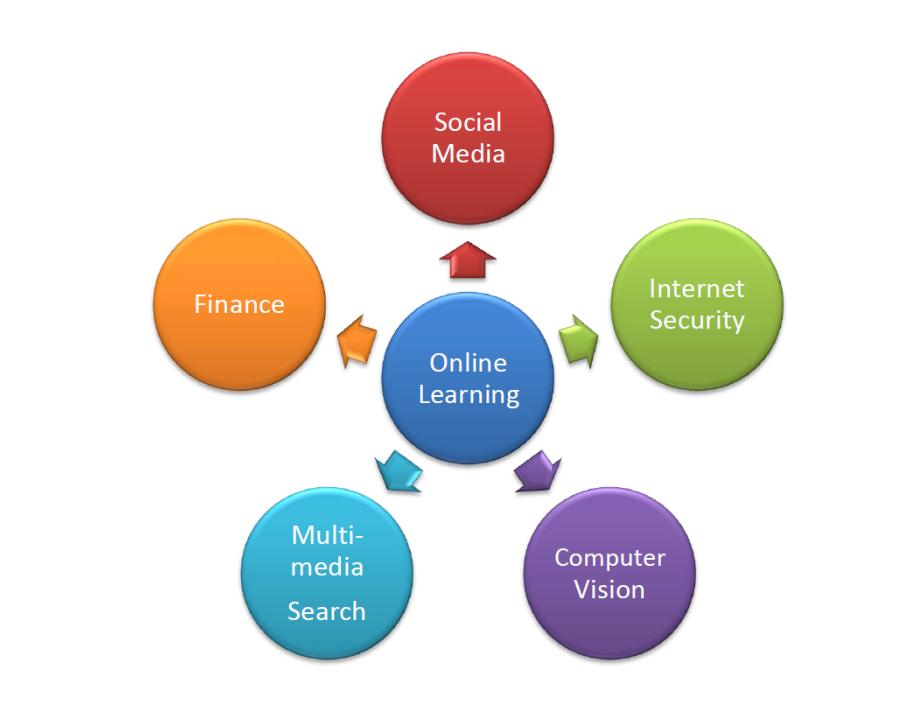
\includegraphics[width=\textwidth, height=\textheight, keepaspectratio]{online-learning-applications}
	\caption{Some areas of application of online learning. Source: \citep{hoi-ol-tutorial}.}
	\label{fig:online-learning-applications}
\end{figure}

Starting with social media, online learning is employed as a mining tool for social media streams to gather business intelligence, such as public emotion and product/brand sentiment. In internet security, it is used as an online anomaly detection mechanism, ranging from spam email detection to the identification of fraudulent credit card transactions. In computer vision, it enables real-time object tracking for video surveillance purposes, especially for the detection of anomalous events from realtime video streams. On the other hand, interactive image/video search via online relevance feedback is one of the various applications of online learning to multimedia search. Finally, in finance, online portfolio selection has recently been demonstrated to outperform traditional benchmarks \citep{olps-survey}. As we already hinted, online methods are crucial in this field, as sequential decisions need to be promptly taken regarding the allocation of wealth among different assets.




\section{Problem Statement and Related Theory}

We first give a formal formulation of online linear regression, which will be our main subject of focus throughout this thesis, and then introduce the basics of statistical learning theory and online convex optimisation as the theoretical foundations for online learning techniques.


\subsection{Online linear regression}

Online learning operates on a sequence of data examples with timestamps. At each step $t$, the learner receives an instance $\mathbf{x}_t \in \mathbb{R}^n$. It first attempts to make a prediction for the output of the incoming instance which, in the case  of linear regression, takes the form $\hat{y}_t = \mathbf{w}_t^\text{T} \mathbf{x}_t$, where $\mathbf{w}_t \in \mathbb{R}^n$ is the incrementally learned weight vector. After making the prediction, the true output $y_t \in \mathbb{R}$ is revealed, and the learner then computes the incurred loss $\ell(y_t, \hat{y}_t) \in \mathbb{R}_{\geq 0}$, based on some criterion to measure the difference between the learner’s prediction and the revealed true output. Using this loss, the learner finally decides whether and how to update the regression model at the end of each learning step.

The following algorithmic framework gives an overview of most first-order online learning algorithms for linear regression, where $\Delta(\mathbf{w}_t; (\mathbf{x}_t, y_t))$ denotes the update of the regression models. Different online learning algorithms operate under different definitions, and designs of the loss function $\ell(\cdot)$ and the updating function $\Delta(\cdot)$.
\begin{algorithm}[H]
  \caption{Online learning framework for linear regression}
\label{alg:online-linear-regression}
  \begin{algorithmic}[1]
    \STATE {\bfseries Initialisation:} $\mathbf{w}_1 = \mathbf{0}_{n\times 1}$
    \FOR{$t=1, 2, \ldots, T$}
      \STATE the learner receives an incoming instance $\mathbf{x}_t \in \mathbb{R}^n$
      \STATE the learner predicts the output: $\hat{y}_t = \mathbf{w}_t^\text{T} \mathbf{x}_t$
      \STATE the true output is revealed by the environment: $y_t \in \mathbb{R}$
      \STATE the learner calculates the suffered loss: $\ell(\mathbf{w}_t; (\mathbf{x}_t, y_t))$
    \IF{$\ell(\mathbf{w}_t; (\mathbf{x}_t, y_t)) > 0$}
      \STATE the learner updates the regression model according to
      \begin{equation*}
      	\mathbf{w}_{t+1} = \mathbf{w}_t + \Delta(\mathbf{w}_t; (\mathbf{x}_t, y_t))
      \end{equation*}
    \ENDIF
    \ENDFOR
  \end{algorithmic}
\end{algorithm}
%By running such an algorithm over a sequence of $T$ rounds, the cumulative loss achieved by the algorithm can be measured as $L_T = \sum_{t=1}^T \ell(y_t, \hat{y}_t)$. The classic goal in an online learning task is to minimise the regret of the underlying online learner's predictions against the best fixed model in hindsight, i.e.\
%\begin{equation}
%	R_T = \sum_{t=1}^T \ell(y_t, \mathbf{w}_t^\text{T} \mathbf{x}_t) - \min_{\mathbf{w}} \sum_{t=1}^T \ell(y_t, \mathbf{w}^\text{T} \mathbf{x}_t),
%\end{equation}
%where the second term is the loss suffered by the optimal model $\mathbf{w}^*$, which can only be known in hindsight after seeing all the instances and their corresponding targets. From the theoretical perspective of regret minimisation, if an online algorithm guarantees that its regret is sublinear as a function of $T$, i.e.\ $R_T = o(T)$, it also satisfies the condition $\lim_{T \rightarrow \infty} R(T)/T = 0$, meaning that on average, the learner performs almost as well as the best fixed model in hindsight.
\begin{mccorrection}
By running such an algorithm over a sequence of $T$ rounds, the cumulative loss achieved by the algorithm can be measured as $L_T = \sum_{t=1}^T \ell(y_t, \hat{y}_t)$. The classic goal in an online learning task is to minimise the regret of the underlying online learner's predictions against the best fixed model in hindsight, i.e.\
\begin{equation}
	R_T = \sum_{t=1}^T \ell(y_t, \mathbf{w}_t^\text{T} \mathbf{x}_t) - \min_{\mathbf{w}} \sum_{t=1}^T \ell(y_t, \mathbf{w}^\text{T} \mathbf{x}_t),
\end{equation}
where the second term is the loss suffered by the optimal model $\mathbf{w}^*$, which can only be known in hindsight after seeing all the instances and their corresponding targets. From the theoretical perspective of regret minimisation, the notion of \emph{no regret} means $R_T \leq b(T)$, where $b(T)$ in $o(T)$.
\end{mccorrection}

\subsection{Statistical learning theory}

Statistical learning theory, first introduced in the late 1960's, is one of key foundations for the theoretical analysis of machine learning problems, especially for supervised learning. There are many comprehensive survey articles and books on the subject matter, including the seminal work of Vladimir Vapnik \citep{vapnik98, vapnik99}. In the following, we review some basic concepts.

\subsubsection{Empirical error minimisation}

Assume instance $\mathbf{x}_t$ is generated randomly from a fixed but unknown distribution $P(\mathbf{x})$, and that the corresponding output $y$ is also generated from a fixed but unknown distribution $P(y|\mathbf{x})$. The joint distribution of the data is then $P(\mathbf{x}, y) = P(\mathbf{x}) P(y|\mathbf{x})$. The goal of supervised learning is to find a prediction function $f(\mathbf{x})$ that minimises the expected value of the loss function
\begin{equation}
	R(f) = \int \ell(y, f(\mathbf{x})) \, \mathrm{d} P(\mathbf{x}, y),
\end{equation}
also termed the \emph{true risk} functional. The solution $f^* = \argmin R(f)$ is the optimal predictor.

In general, the true risk functional cannot be computed directly because of the unknown distribution $P(\mathbf{x}, y)$. In practice, we approximate it by estimating the risk over a finite collection of examples $(\mathbf{x}_1, y_1), \ldots, (\mathbf{x}_m, y_m)$, drawn in an i.i.d. fashion. This estimated risk is known as \emph{empirical risk} or \emph{empirical error}, and is given by
\begin{equation}
	R_\text{emp}(f) = \frac{1}{m} \sum_{i=1}^m \ell(y_i, f(\mathbf{x}_i)).
\end{equation}
Learning via empirical risk minimisation (ERM) consists in finding a hypothesis $f$ over a hypothesis space $\mathcal{F}$ by solving
\begin{equation}
	\hat{f}_m = \argmin_{f\in\mathcal{F}} \; R_\text{emp}(f).
\end{equation}
ERM forms the theoretical basis for many machine learning algorithms. In the case of regression, assuming $\mathcal{F}$ is the set of linear regressors and the squared loss is used, the ERM principle suggests that the best linear model $\mathbf{w}^*$ can be learned by minimising the following objective with respect to $\mathbf{w}$:
\begin{equation}
	R_\text{emp}(\mathbf{w}) =  \frac{1}{m} \sum_{i=1}^m (y_i - \mathbf{w}^\text{T}\mathbf{x}_i)^2.
\end{equation}

\subsection{Convex optimisation theory}

Many online learning problems can essentially be (re-)formulated as an online convex optimisation (OCO) task. In the following, we introduce some of the basics of OCO.

An online convex optimisation task typically consists of two major elements: a convex set $\mathcal{S}$ and a convex loss function $\ell_t(\cdot)$. At each time step $t$, the online algorithm picks a weight vector $\mathbf{w}_t \in \mathcal{S}$, after which it suffers a loss $\ell_t(\mathbf{w}_t)$. The goal of the online algorithm is to play a sequence of decisions $\mathbf{w}_1, \mathbf{w}_2, \ldots$ so as to minimise the regret in hindsight.

More formally, an online algorithm aims to achieve a low regret $R_T$ after $T$ rounds, where the regret $R_T$ is defined as
\begin{equation}
\label{eq:regret}
	R_T = \sum_{t=1}^T \ell_t(\mathbf{w}_t) - \inf_{\mathbf{w}^* \in \mathcal{S}} \sum_{t=1}^T \ell_t(\mathbf{w}^*).
\end{equation}
In an online linear regression task on a sequence of examples $(\mathbf{x}_t, y_t)$, $t=1,\ldots,T$, with $\mathbf{x}_t \in \mathbb{R}^n$ and $y_t \in \mathbb{R}$, a commonly used loss function is the squared loss $\ell_t(\mathbf{w}) = (y_t - \mathbf{w}^\text{T}\mathbf{x}_t)^2$. In this case, the convex set $\mathcal{S}$ would be $\mathbb{R}^n$. There are a variety of algorithms to solve this problem.

Below, we briefly discuss two major families of OCO methods, namely first-order and second-order algorithms that will play an instrumental role in the development of our research work. For a comprehensive treatment of the subject, the interested reader is referred to the books by \citet{shalev-shwartz11, oco}.

\section{First-Order Online Learning}

\begin{mccorrection}
First-order methods aim to minimise the regret in Eq. \eqref{eq:regret} using first-order gradient information. The majority of first-order algorithms are classification algorithms. Only a few have been developed for regression tasks, such as online gradient descent \citep{ogd} and online passive-aggressive regression \citep{crammer06}. We describe these below.
\end{mccorrection}

\subsection{Online passive-aggressive regression}

Online passive-aggressive (PA) regression is a popular online regression algorithm that was introduced in \citep{crammer06}. It has been applied across a number of diverse areas, including online portfolio selection \citep{pamr}, non-negative matrix factorisation and completion \citep{blondel14}, and statistical machine translation \citep{turchi}.

On every round, the PA regression algorithm receives an instance $\mathbf{x}_t$ and predicts a target value $\hat{y}_t = \mathbf{w}_{t}^\text{T}\mathbf{x}_t$ using its internal regression function. After making a prediction, the algorithm is given
the true target value $y_t$ and suffers an instantaneous loss. PA regression relies on the $\epsilon$-insensitive loss function (ILF) \citep{vapnik98}, defined as
\begin{equation}
\label{eq:ilf}
	 \ell_{\epsilon}(\mathbf{w}; \mathbf{z}) \equiv
	 \begin{cases}
	 	0 & \text{if } |y - \mathbf{w}^\text{T}\mathbf{x}| \leq \epsilon \\
	 	|y - \mathbf{w}^\text{T}\mathbf{x}| - \epsilon & \text{otherwise}
	 \end{cases},
\end{equation}
where $\mathbf{z} = (\mathbf{x}, y)$ and $\epsilon$ is a positive hyperparameter that controls the algorithm's sensitivity to prediction mistakes. The ILF is zero when the predicted target deviates from the true target by less than $\epsilon$ units, and otherwise grows linearly with $|y_t - \hat{y}_t|$. At the end of every round, the algorithm uses $\mathbf{w}_t$ and the example $\mathbf{z}_t$ to generate a new weight vector $\mathbf{w}_{t+1}$, which is then used to extend the prediction on the next round.

We now describe how the PA regression algorithm sequentially updates its weight vector. The latter is initialised to the zero vector. Then, on each subsequent round, the algorithm sets the new weight vector to be
\begin{equation}
\label{eq:generic-pa-optpb}
	\mathbf{w}_{t+1} = \argmin_{\mathbf{w} \in \mathbb{R}^n} \; \frac{1}{2}\Vert\mathbf{w} - \mathbf{w}_t\Vert_2^2
	\qquad \text{s.t.} \qquad \ell_{\epsilon}(\mathbf{w}; \mathbf{z}_t) = 0.
\end{equation}
The set $C_{\epsilon}(\mathbf{z}_t) \equiv \{\mathbf{w} \in \mathbb{R}^n : \ell_{\epsilon}(\mathbf{w}; \mathbf{z}_t) = 0\}$ is a hyper-slab of width $2\epsilon$. Geometrically, the PA algorithm for regression projects $\mathbf{w}_t$ onto this hyper-slab at the end of every round, unless $\mathbf{w}_t$ suffers no loss from the new data, i.e.\ $\mathbf{w}_t \in C_{\epsilon}(\mathbf{z}_t)$. These mechanics are illustrated in Figure~\ref{fig:pa-illustration}.
\begin{figure}[t]
	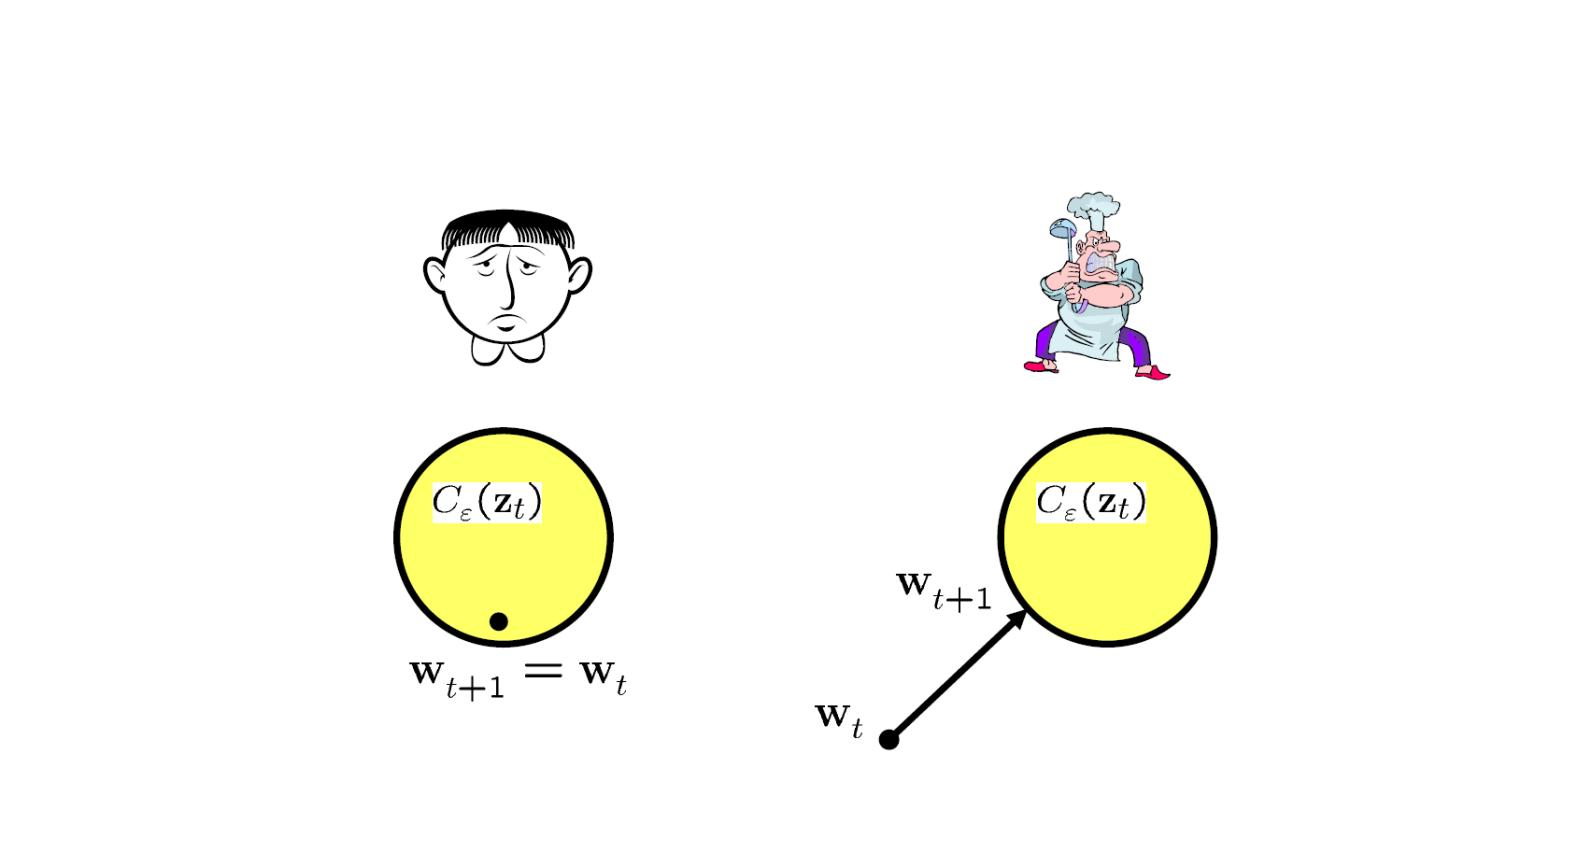
\includegraphics[width=\textwidth, height=\textheight, keepaspectratio]{pa-illustration}
	\caption{The mechanics of linear PA regression. The algorithm \emph{passively} assigns $\mathbf{w}_{t+1} = \mathbf{w}_t$ as long as $\mathbf{w}_t$ incurs no loss on the incoming example $\mathbf{z}_t$. Otherwise, it \emph{aggressively} projects $\mathbf{w}_t$ onto the feasible set $C_{\epsilon}(\mathbf{z}_t)$ of weight vectors which attain zero loss. Source: \url{https://home.ttic.edu/~shai/ppt/PassiveAggressive.ppt}.}
	\label{fig:pa-illustration}
\end{figure}

Using the shorthand $\ell_t = \ell_{\epsilon}(\mathbf{w}; \mathbf{z}_t)$, \citet{crammer06} showed that the update in Eq. \eqref{eq:generic-pa-optpb} has a closed-form solution, namely
\begin{equation}
\label{eq:generic-pa-update-rule}
	\mathbf{w}_{t+1}
	= \mathbf{w}_t + \tau_t\mathbf{v}_t,
\end{equation}
where $\tau_t = \ell_t / \Vert\mathbf{x}_t\Vert_2^2$ is the Lagrange multiplier associated with the feasibility constraint $\mathbf{w}_{t+1} \in C_{\epsilon}(\mathbf{z}_t)$, and $\mathbf{v}_t \equiv \mathrm{sgn}(y_t - \hat{y}_t)\mathbf{x}_t$ represents the direction of the update.

\subsubsection{Soft-margin PA regression}

As discussed above, the PA algorithm employs an aggressive update strategy, by modifying the weight vector by as much as needed to satisfy the constraint imposed by the current example. In certain real-life situations, this strategy may also result in undesirable consequences. Consider for instance the common phenomenon of outliers. An outlier may cause the PA algorithm to drastically change its weight vector in the wrong direction. A single outlier may thereby lead to several prediction mistakes on subsequent rounds.

To cope with such problems, \citet{crammer06} developed two variations on the PA update that employ gentler update strategies. These variations are based on the technique previously used to derive soft-margin classifiers \citep{vapnik98}: they introduce a non-negative slack variable $\xi$ into the optimisation problem defined in Eq. \eqref{eq:generic-pa-optpb}. This variable can be introduced in two different ways. First, we consider the update where the objective function scales linearly with $\xi$:
\begin{equation}
\label{eq:paI-optpb}
	\mathbf{w}_{t+1} = \argmin_{\mathbf{w},\, \xi} \; \Big\{\frac{1}{2}\Vert\mathbf{w} - \mathbf{w}_t\Vert_2^2 \, + \, C\xi\Big\}
	\qquad \text{s.t.} \qquad \ell_{\epsilon}(\mathbf{w}; \mathbf{z}_t) \leq \xi \quad \text{and} \quad \xi \geq 0.
\end{equation}
Here, $C$ is a positive parameter which controls the influence of the slack term on the objective function. Specifically, larger values of $C$ imply a more aggressive update, and $C$ is therefore referred to as the \emph{aggressiveness parameter} of the algorithm. This variant of PA regression is known as \emph{PA-I}.

Alternatively, the objective function scales quadratically with $\xi$, resulting in the following constrained optimisation problem:
\begin{equation}
\label{eq:paII-optpb}
	\mathbf{w}_{t+1} = \argmin_{\mathbf{w},\, \xi} \; \Big\{\frac{1}{2}\Vert\mathbf{w} - \mathbf{w}_t\Vert_2^2 \, + \, C\xi^2\Big\}
	\qquad \text{s.t.} \qquad \ell_{\epsilon}(\mathbf{w}; \mathbf{z}_t) \leq \xi.
\end{equation}
Note that the constraint $\xi \geq 0$ which appears in Eq. \eqref{eq:paI-optpb} is no longer necessary, since $\xi^2$ is always non-negative. The algorithm that results from this update is termed \emph{PA-II}. As with PA-I, $C$ is a positive
parameter which governs the extent to which the PA-II update is aggressive.

As shown in \citep{crammer06}, the updates of PA-I and PA-II share the simple analytical solution $\mathbf{w}_{t+1} = \mathbf{w}_t + \tau_t \mathbf{v}_t$, as defined in Eq. \eqref{eq:generic-pa-update-rule}, but with the following Lagrange multipliers, respectively:
\begin{equation}
	\tau_t = \min\bigg\{C, \; \frac{\ell_t}{\Vert\mathbf{x}_t\Vert_2^2}\bigg\} \quad (\text{PA-I})
	\qquad \text{and} \qquad
	\tau_t = \frac{\ell_t}{\Vert\mathbf{x}_t\Vert_2^2 \, + \, \frac{1}{2C}} \quad (\text{PA-II}).
\end{equation}
All PA variants are outlined in Algorithm~\ref{alg:pa}.
\begin{algorithm}[H]
  \caption{Passive-Aggressive Algorithms}
\label{alg:pa}
  \begin{algorithmic}[1]
    \STATE {\bfseries Initialisation:} $\mathbf{w}_1 = \mathbf{0}_{n\times 1}$, insensitivity parameter $\epsilon \geq 0$, aggressiveness parameter $C > 0$
    \FOR{$t=1, 2, \ldots, T$}
      \STATE receive $\mathbf{x}_t \in \mathbb{R}^n$, predict $\hat{y}_t$ using $\mathbf{w}_t$
      \STATE suffer loss $\ell_t(\mathbf{w}_t)$
      \STATE set
      \begin{equation*}
      	\tau_t = 
      	\begin{cases}
      		\ell_t / \Vert\mathbf{x}_t\Vert_2^2 & \text{(PA)} \\
      		\min\{C,\, \ell_t / \Vert\mathbf{x}_t\Vert_2^2\}  & \text{(PA-I)} \\
      		\frac{\ell_t}{\Vert\mathbf{x}_t\Vert_2^2 \, + \, \frac{1}{2C}} & \text{(PA-II)} \\
      	\end{cases}
      \end{equation*}
    \STATE update $\mathbf{w}_{t+1} = \mathbf{w}_t + \tau_t \mathbf{v}_t$, where $\mathbf{v}_t = \mathrm{sgn}(y_t - \hat{y}_t)\mathbf{x}_t$
    \ENDFOR
  \end{algorithmic}
\end{algorithm}
%\paragraph{Relationship between PA-I and support vector regression}
%
%It is worthwhile noting that the PA-I optimisation problem in Eq. \eqref{eq:paI-optpb} is analogous to that which arises in $\epsilon$-support vector regression (SVR) \citep{vapnik98}. Indeed, the core of its construction can be viewed as finding a linear SVR on a single example, while replacing the norm constraint of SVR with a proximity constraint to the current weight vector.

\subsection{Online gradient descent}

As we mentioned earlier, many online learning problems can be formulated as an online convex optimisation (OCO) task, which can be solved by applying the online gradient descent (OGD) algorithm. The latter is perhaps the simplest algorithm that applies to the most general OCO setting. Based on standard gradient descent from offline optimisation, it was introduced in its online form by Martin Zinkevich \citep{ogd}. The pseudo-code for the algorithm is given in Algorithm~\ref{alg:ogd}.
\begin{algorithm}[H]
  \caption{Online Gradient Descent}
\label{alg:ogd}
  \begin{algorithmic}[1]
    \STATE {\bfseries Initialisation:} convex set $\mathcal{K}$, horizon $T$, $\mathbf{x}_1 \in \mathcal{K}$, learning-rate schedule $\{\eta_t\}$
    \FOR{$t=1, 2, \ldots, T$}
      \STATE play $\mathbf{x}_t$ and observe cost $f_{t}(\mathbf{x}_t)$
      \STATE update and project:
      \begin{align*}
      	\mathbf{y}_{t+1} &= \mathbf{x}_t - \eta_t \nabla f_{t}(\mathbf{x}_t) \\
      	\mathbf{x}_{t+1} &= \Pi_{\mathcal{K}}(\mathbf{y}_{t+1}) \equiv \argmin_{\mathbf{x} \in \mathcal{K}} \; \Vert\mathbf{x} - \mathbf{y}_{t+1}\Vert_2
      \end{align*}
    \ENDFOR
  \end{algorithmic}
\end{algorithm}

At each iteration, the algorithm takes a step from the previous point in the direction of the gradient of the previous cost. This step may result in a point outside of the underlying convex set. In such cases, the algorithm projects the point back onto the convex set, i.e.\ finds its closest point in the convex set. Despite the fact that the next cost function may be completely different from the costs observed thus far, the regret attained by the algorithm is sublinear (see \citep[Theorem~3.1.]{oco}). A conceptual illustration of the algorithm is given in Figure~\ref{fig:ogd}.
\begin{figure}[t]
	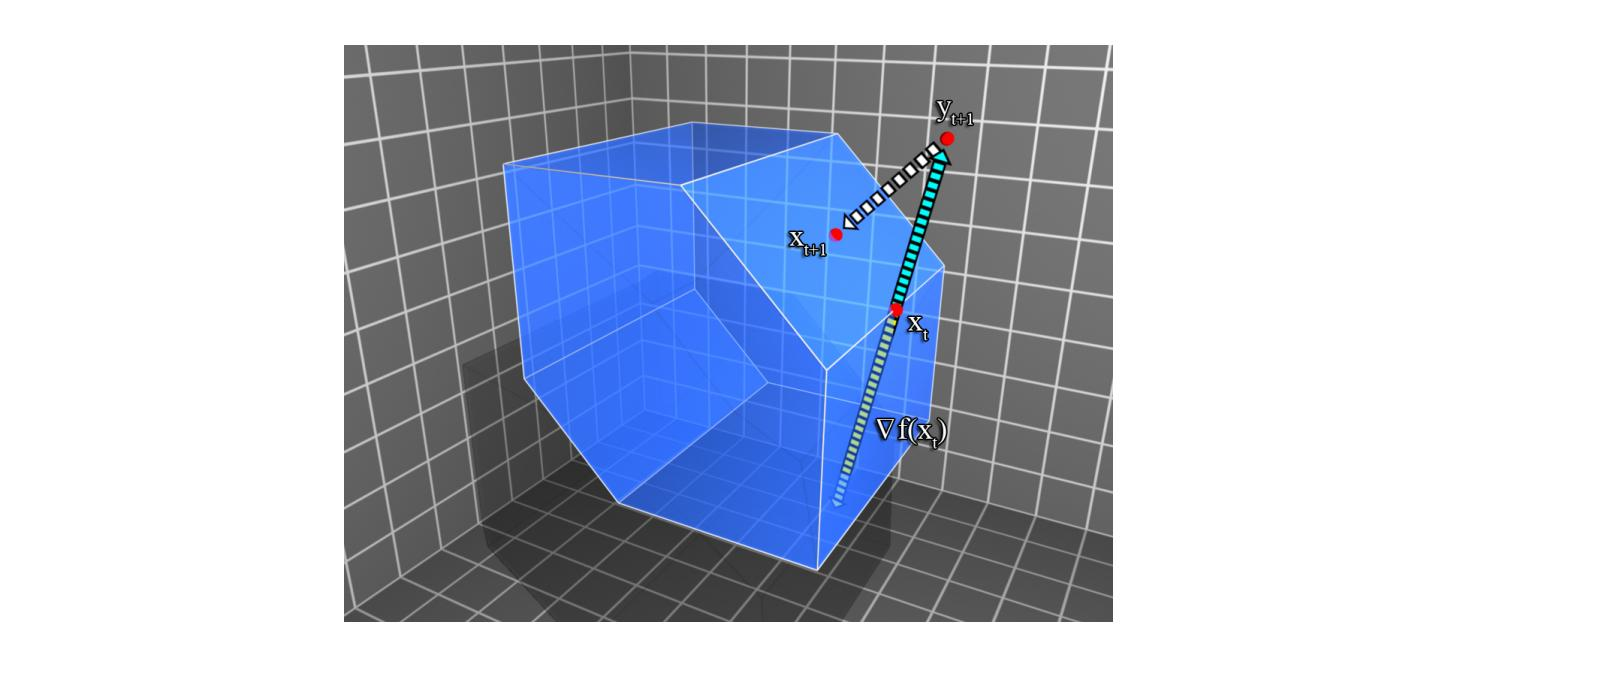
\includegraphics[width=\textwidth, height=\textheight, keepaspectratio]{ogd}
	\caption{Online gradient descent: the iterate $\mathbf{x}_{t+1}$ is derived by moving $\mathbf{x}_t$ into the direction of the current gradient $\nabla f_t(\mathbf{x}_t)$, then projecting it back onto $\mathcal{K}$. Source: \citep{oco}.}
	\label{fig:ogd}
\end{figure}

In the case of linear regression with a squared loss function, the update rule for OGD takes the form
\begin{equation}
	\mathbf{y}_{t+1} = \mathbf{x}_t - 2\eta_t (\hat{y}_t - y_t)\mathbf{x}_t.
\end{equation} 
In general, this rule is straightforward to implement, and takes linear time. OGD and PA share similar update rules, but differ in that OGD often employs some predefined learning-rate scheme, whereas PA chooses the optimal learning rate $\tau_t$ at each round (albeit subject to a predefined cost parameter $C$).
%In the literature, different OGD variants have been proposed to improve either theoretical bounds or practical issues, such as adaptive OGD (Hazan et al., 2007b), and mini-batch OGD (Dekel et al., 2012), amongst others. 




\section{Second-Order Online Learning}

%Unlike first-order online learning algorithms which only exploit the first-order information contained in the gradient for the purpose of solving online optimisation tasks, second-order online learning algorithms exploit both first-order and second-order information in order to speed up convergence. Despite their superior learning performance, a major drawback of second-order algorithms is their higher computational complexity. In what follows, we briefly describe some popular second-order online learning algorithms.

To improve the efficacy of first-order learning methods, recent years have witnessed the active development of second-order online learning algorithms. In general, these algorithms place a Gaussian prior distribution over the weights, with mean vector $\boldsymbol{\mu} \in \mathbb{R}^n$ and covariance matrix $\boldsymbol{\Sigma} \in \mathbb{R}^{n \times n}$. The model parameters are updated in the online learning process.

Examples of second-order algorithms for linear regression include adaptive regularisation of weight vectors \citep{arow}, which was inspired by confidence-weighted learning \citep{dredze08}, and a more recently introduced Bayesian treatment of online PA learning, namely online Bayesian passive-aggressive learning \citep{bayespa}.

\subsection{Confidence-weighted learning}

Confidence-weighted (CW) learning was introduced in \citep{dredze08} as a probabilistic extension of online passive-aggressive learning that takes into account model/parameter uncertainty by maintaining a probabilistic measure of confidence in each weight. Less confident weights are updated more aggressively than more confident ones. Weight confidence is formalised with a Gaussian distribution over weight vectors, which is updated for each new training instance so that the probability of correct classification for that instance under the updated distribution meets a specified confidence.

In the CW framework, the linear classifier is modelled with a Gaussian distribution, i.e.\ $\mathbf{w} \sim \mathcal{N}(\boldsymbol{\mu},\, \boldsymbol{\Sigma})$. Given an instance $\mathbf{x}$, the label is then predicted according to the sign of $\mathbf{w}^\text{T}\mathbf{x}$. The multivariate Gaussian distribution over weight vectors induces a univariate Gaussian distribution over the margin viewed as a random variable. Specifically:
\begin{equation}
	M \equiv y(\mathbf{w}^\text{T}\mathbf{x}) \sim \mathcal{N}(y(\boldsymbol{\mu}^\text{T}\mathbf{x}),\, \mathbf{x}^\text{T}\boldsymbol{\Sigma}\mathbf{x}).
\end{equation}


Following the intuition underlying the PA algorithms, the CW algorithm chooses the distribution closest in the KL divergence sense to the current distribution $\mathcal{N}(\boldsymbol{\mu}_t,\, \boldsymbol{\Sigma}_t)$. Thus, on round $t$, the algorithm sets the parameters of the distribution by solving the following convex optimisation problem:
\begin{align}
	\mathcal{N}(\boldsymbol{\mu}_{t+1},\, \boldsymbol{\Sigma}_{t+1})
	&= \min \quad \mathrm{KL}\big[\mathcal{N}(\boldsymbol{\mu},\, \boldsymbol{\Sigma}) \, \Vert \, \mathcal{N}(\boldsymbol{\mu}_t,\, \boldsymbol{\Sigma}_t)\big]
	\\ \nonumber
	& \text{s.t.} \qquad \mathbb{P}\Big\{y_{t}(\mathbf{w}^\text{T}\mathbf{x}_{t}) \geq 0\Big\} \geq \eta.
\end{align}
In plain English, this means that the new distribution should remain as close as possible to the previous distribution so that the classifier does not forget the information learnt from previous instances. The constraint reflects the fact that the new classifier should classify the new instance $\mathbf{x}_t$ correctly with probability higher than a predefined threshold parameter $\eta \in (0, 1)$.

Note that this is only the basic form of confidence weighted algorithms and has several drawbacks: i) similar to the hard-margin PA algorithm, the constraint forces the new instance to be correctly classified, which makes this algorithm very sensitive to noise; ii) the constraint is expressed in terms of a probability. It is easy to solve a problem with a constraint of the form $g(\boldsymbol{\mu}, \boldsymbol{\Sigma}) < 0$. However, a problem with a constraint on a probability is only solvable when the distribution is known. Thus, this method is hardly generalisable to other online learning tasks for which the constraint does not follow a Gaussian distribution.

\subsection{Adaptive regularisation of weights}

Confidence-weighted algorithms have been shown to perform well in practice (see, e.g., \citep{dredze08}), but they suffer from several problems. First, the update is quite aggressive, forcing the probability of predicting each example correctly to be at least $\eta > 1/2$ regardless of the cost to the objective. This may cause severe over-fitting when labels are noisy, especially considering the fact that the CW framework assumes that the data are linearly separable. Second, they are designed for classification, and it is not clear how to extend them to alternative settings such as regression. This is in part because the constraint is written in discrete terms where the prediction is either correct or no.

Adaptive regularisation of weights (AROW) is a variant of CW that was proposed by \citet{arow} to deal with both of the aforementioned issues, coping more effectively with label noise and generalising the advantages of CW learning in an extensible way. Like CW, AROW maintains a Gaussian distribution over weight vectors, with mean $\boldsymbol{\mu}$ and covariance $\boldsymbol{\Sigma}$. However, it expresses the CW constraint in terms of a set of regularisers, minimising the following unconstrained objective on each round:
\begin{equation}
	\mathcal{C}(\boldsymbol{\mu}, \boldsymbol{\Sigma})
	= \mathrm{KL}\big[\mathcal{N}(\boldsymbol{\mu},\, \boldsymbol{\Sigma}) \, \Vert \, \mathcal{N}(\boldsymbol{\mu}_t,\, \boldsymbol{\Sigma}_t)\big]
	+ \lambda_1 \ell_{\mathrm{h}^2}(y_t, \boldsymbol{\mu}^\text{T}\mathbf{x}_t) + \lambda_2 \mathbf{x}_t^\text{T}\boldsymbol{\Sigma}\mathbf{x}_t,
\end{equation}
where $\ell_{\mathrm{h}^2}(y_t, \boldsymbol{\mu}^\text{T}\mathbf{x}_t) = (\max\{0, \, 1 - y_t(\boldsymbol{\mu}^\text{T}\mathbf{x}_t)\})^2$ is the squared-hinge loss suffered using the weight vector $\boldsymbol{\mu}$ to predict the output for input $\mathbf{x}_t$ when the true output is $y_t$, and $\lambda_1, \lambda_2 \geq 0$ are two trade-off hyperparameters.

The objective balances three desires. First, the parameters should not change radically on each round, since the current parameters contain information about previous examples (first term). Second, the new mean parameters should predict the current example with low loss (second term). Finally, as we see more examples, our confidence in the parameters should generally grow (third term).

Besides the robustness to noisy data, another important advantage of AROW is its ability to be easily generalised to other online learning tasks. Of particular interest to us is online linear regression. Applying the ideas behind AROW to regression problems turns out to yield the well-known recursive least squares (RLS) algorithm \citep{haykin}, for which AROW offers new bounds.


\subsection{Online Bayesian passive-aggressive regression}

Though enjoying strong discriminative ability suitable for predictive tasks, the online PA regression framework is formulated as a point-estimate problem optimising some deterministic objective function. This may lead to some inconvenience. On the one hand, PA makes point rather than probabilistic predictions, thereby failing to explicitly account for model/prediction uncertainty. On the other hand, the estimated single large-margin model is often less than sufficient to describe complex data, such as those with rich underlying structures. Online Bayesian passive-aggressive regression (BayesPA) was introduced to effectively address these shortcomings \citep{bayespa}.

Instead of updating a point estimate of $\mathbf{w}$, BayesPA sequentially infers a new post-data posterior distribution $q_{t+1}(\mathbf{w})$, either parametric or nonparametric, on the arrival of new data $(\mathbf{x}_t, y_t)$ by solving
the following optimisation problem\footnote{Here we consider the soft-margin version of BayesPA.}:
\begin{equation}
\label{eq:bayespa-optpb}
%	\min_{q(\mathbf{w}) \in \mathcal{P}} \; \Big\{\mathrm{KL}[q(\mathbf{w}) \, \Vert \, q_{t}(\mathbf{w})] - \mathbb{E}_{q(\mathbf{w})}[\log p(\mathbf{x}_t|\mathbf{w})]\Big\}
%	\quad \text{s.t.} \quad \ell_{\epsilon}(q(\mathbf{w}); (\mathbf{x}_t, y_t)) = 0,
	q_{t+1}(\mathbf{w}) = \argmin_{q(\mathbf{w}) \in \mathcal{F}_t} \; \Big\{\mathrm{KL}[q(\mathbf{w}) \, \Vert \, q_{t}(\mathbf{w})] + 2C \, \ell_{\epsilon}(q(\mathbf{w}); \mathbf{x}_{t+1}, y_{t+1})\Big\},
\end{equation}
where $\mathcal{P}$ is the probability simplex, $\ell_{\epsilon}(q(\mathbf{w}); \mathbf{x}_{t+1}, y_{t+1})$ is the expected $\epsilon$-insensitive loss, and $C$ is the parameter for balancing the loss of newly estimated distribution on new data and the similarity between the new distribution and the distribution estimated at time $t$ (the constant 2 is just for convenience in the subsequent inference). In other words, the algorithm finds a post-data posterior distribution $q_{t+1}(\mathbf{w})$ in the feasible zone that is not only close to the current weight distribution $q_{t}(\mathbf{w})$ in terms of the KL divergence, but also has a high likelihood of explaining the data.

By defining
$
	\ell_{\epsilon}(q(\mathbf{w}); \mathbf{x}_{t+1}, y_{t+1})
	\equiv \mathbb{E}_{q(\mathbf{w})}[\max\{0,\, |y_{t+1} - \mathbf{w}^\text{T}\mathbf{x}_{t+1}| - \epsilon\}],
$
then expanding the KL divergence in Eq. \eqref{eq:bayespa-optpb} and reorganising terms, we obtain the following closed-form update rule for BayesPA:
\begin{equation}
	q_{t+1}(\mathbf{w}) = \frac{q_{t}(\mathbf{w})\exp\{-2C\max\{0,\, |y_{t+1} - \mathbf{w}^\text{T}\mathbf{x}_{t+1}| - \epsilon\}\}}{Q(\mathbf{x}_{t+1}, y_{t+1})},
\end{equation}
where $Q(\mathbf{x}_{t+1}, y_{t+1})$ is a normalisation constant (see \citep[Lemma~4]{bayespa} for a proof).
\chapter{Online Portfolio Selection}
\label{ch:olps}

\minitoc




Online portfolio selection is a fundamental problem in computational finance, which has been extensively studied across several research communities, including finance, statistics, artificial intelligence, machine learning, and data mining. This chapter -- a summarised version of \citep{olps-survey} -- aims to provide an overview and structural understanding of the most well-known techniques used in the literature.
%We first formulate online portfolio selection as a sequential decision problem, and then survey a variety of state-of-the-art approaches grouped into several categories, including benchmark, follow-the-winner, follow-the-loser, pattern-matching and meta-learning algorithms. In addition to the problem formulation and related algorithms, we cover the relationship between these algorithms and capital growth theory so as to better understand their similarities and differences. Finally, we discuss some open issues and evaluate some emerging new trends for future research.




\section{Introduction}

Portfolio selection aims to optimise the allocation of wealth across a set of assets, and is considered a fundamental research problem in computational finance. There are two major schools of thought: \emph{i}) mean-variance theory \citep{markowitz52, markowitz59, markowitz00} which originated in the finance community, and \emph{ii}) capital growth theory (CGT) \citep{kelly, hakansson95} which has its roots in information theory. Mean-variance theory, widely known in the asset management industry, focuses on single-period (batch) portfolio selection and trades off a portfolio's expected return (mean) vs its risk (variance), which typically determines the optimal portfolios subject to the investor's risk-return profile. CGT, on the other hand, focuses on multiple-period or sequential portfolio selection, seeking to maximise the portfolio's expected growth rate, or expected log return. Although both theories solve the task of portfolio selection, the latter is more aligned with the `online' scenario, which naturally consists of multiple periods and is the focus of this thesis.

The goal of online portfolio selection is to sequentially select a portfolio of assets so as to achieve certain targets. Several algorithms have been proposed to solve this task and can be broadly grouped into three categories, namely \emph{follow the winner}, \emph{follow the loser} and \emph{pattern matching}. In the spirit of CGT, follow-the-winner algorithms try to asymptotically achieve the same growth rate (expected log return) as that of an optimal strategy. In contrast, follow the loser strategies transfer wealth from overperforming to underperforming assets, which may seem counterintuitive, but often leads to significantly better performance in practice. The third category, the pattern-matching approach, tries to predict the next market distribution based on historical data, and explicitly optimises the portfolio based on the sampled distribution. Although these three categories are focused on a single strategy (class), there is another category that combines multiple strategies (classes), known as \emph{meta-learning algorithms}. Table~\ref{tab:olps-algos} outlines the main algorithms and corresponding references.
\begin{table}[H]
\caption{Taxonomy of online portfolio selection techniques. Source: \citep{olps-survey}.}
\label{tab:olps-algos}
\centering
\resizebox{\textwidth}{!}{
\begin{tabular}{ |l|l|l|l| } 
\hline
Category & Algorithms & Representative References \\
\hline
\multirow{3}{10em}{Benchmarks} & Buy and Hold & \\ 
& Best Stock &  \\ 
& Constant Rebalanced Portfolios & \citep{kelly, cover} \\ 
\hline
\multirow{5}{10em}{Follow the winner} & Universal Portfolios & \citep{cover, cover96} \\ 
& Exponential Gradient & \citep{eg} \\ 
& Follow the Leader & \citep{gaivoronski00} \\
& Follow the Regularized Leader & \citep{ons} \\
& Aggregating-Type Algorithms & \citep{vovk98} \\ 
\hline
\multirow{5}{10em}{Follow the loser} & Anti-Correlation & \citep{borodin04} \\ 
& Passive-Aggressive Mean Reversion & \citep{pamr} \\ 
& Confidence-Weighted Mean Reversion & \citep{cwmr} \\
& Online Moving Average Reversion & \citep{olmar} \\
& Robust Median Reversion & \citep{rmr} \\ 
\hline
\multirow{9}{10em}{Pattern matching} & Nonparametric Histogram Log-Optimal Strategy & \citep{bnn} \\ 
& Nonparametric Kernel-Based Log-Optimal Strategy & \\ 
& Nonparametric Nearest Neighbor Log-Optimal Strategy & \citep{bnn2} \\
& Correlation-Driven Nonparametric Learning Strategy & \citep{corn} \\
& Nonparametric Kernel-Based Semi-Log-Optimal Strategy & \citep{gyorfi07} \\
& Nonparametric Kernel-Based Markowitz-Type Strategy & \citep{ottucsak07} \\ 
& Nonparametric Kernel-Based GV-Type Strategy & \citep{gyorfi08} \\ 
\hline
\multirow{5}{10em}{Meta learning} & Aggregating Algorithm & \citep{vovk90, vovk98} \\ 
& Fast Universalization Algorithm & \citep{akcoglu02, akcoglu04} \\ 
& Online Gradient Updates & \\
& Online Newton Updates & \citep{das11} \\
& Follow the Leading History & \citep{hazan09} \\
\hline
\end{tabular}
}
\end{table}

This chapter provides a fairly detailed description of the algorithms mentioned in Table~\ref{tab:olps-algos}. The remainder of the chapter is structured as follows. Section~\ref{sec:problem-setting} formally posits the problem of online portfolio selection and discusses several practical issues. Section~\ref{sec:olps-approaches} introduces the state-of-the-art algorithms, including benchmarks in Section~\ref{sec:benchmarks}, follow-the-winner approaches in Section~\ref{sec:follow-the-winner}, follow-the-loser strategies in Section~\ref{sec:follow-the-loser}, pattern-matching approaches in Section~\ref{sec:pattern-matching}, and meta-learning algorithms in Section~\ref{sec:mlas}. Finally, Section~\ref{sec:conclusion} concludes this chapter.




\section{Problem Setting}
\label{sec:problem-setting}

We now formally describe the online portfolio selection (OLPS) problem. Consider an investment task over a financial market with $m$ assets and a $T$-period horizon. On the $t$-th period, the asset prices are represented by a \emph{closing-price vector} $\mathbf{p}_t \in \mathbb{R}^m_+$. The price changes are represented by a \emph{price-relative vector} $\mathbf{x}_t \in \mathbb{R}_+^m$ such that $x_{t,i} \equiv \frac{p_{t,i}}{p_{t-1,i}}$ for each asset $i \in [m]$. Thus, an investment in asset $i$ on the $t$-th period increases by a factor of $x_{t,i}$. Let us denote by $\mathbf{x}_{t_1:t_2} \equiv \{\mathbf{x}_{t_1}, \mathbf{x}_{t_1+1}, \ldots, \mathbf{x}_{t_2}\}$ a sequence of price-relative vectors ranging from period $t_1$ to $t_2$. Therefore, $\mathbf{x}_{1:T} = \{\mathbf{x}_{1}, \mathbf{x}_{2}, \ldots, \mathbf{x}_{T}\}$ represents the sequence of price-relative vectors over the entire $T$-period horizon.

An investment on the $t$-th period is specified by a \emph{portfolio vector} $\mathbf{b}_t = (b_{t,1}, \ldots, b_{t,m})$, where $b_{t,i}$ represents the proportion of wealth invested in asset $i$. Typically, we assume the portfolio is self-financed and that no margin/short sale is allowed, so that each entry of a portfolio is non-negative and all entries add up to one:
\begin{equation}
	\mathbf{b}_t \in \Delta_m
	\equiv \Big\{\mathbf{b}_t : \mathbf{b}_t \in \mathbb{R}^m_+,\, \sum_{i =1}^m b_{t,i} = 1\Big\}.
\end{equation}
The investment procedure is represented by a \emph{portfolio strategy} such that $\mathbf{b}$ is initialised at the equally-weighted portfolio by convention, that is $\mathbf{b}_1 = \mathbf{1}/m$, followed by a sequence of mappings $\mathbf{b}_t : \mathbb{R}^{m(t-1)}_{+} \rightarrow \Delta_m$ for $t = 2, 3, \ldots$, where $\mathbf{b}_t = \mathbf{b}_t(\mathbf{x}_{1:t-1})$ is the $t$-th portfolio given the historical market sequence $\mathbf{x}_{1:t-1} = \{\mathbf{x}_1, \ldots, \mathbf{x}_{t-1}\}$. We denote by $\mathbf{b}_{1:T} = \{\mathbf{b}_1, \ldots, \mathbf{b}_T\}$ the strategy for $T$ periods.

On the $t$-th period, a portfolio $\mathbf{b}_t$ produces a \emph{portfolio period return} $s_t$, that is, the wealth increases by a factor of $s_t \equiv \mathbf{b}_t^\text{T}\mathbf{x}_t = \sum_{i=1}^m b_{t,i}x_{t,i}$. We shall assume all profits are reinvested, which implies that wealth grows in a multiplicative fashion. Thus, after $T$ periods, a portfolio strategy $\mathbf{b}_{1:T}$ produces a \emph{portfolio cumulative wealth} of $S_T$, which amounts to the initial wealth times a factor of $\prod_{t=1}^T s_t$, that is
\begin{equation}
\label{eq:portfolio-cumulative-wealth}
	S_T(\mathbf{b}_{1:T})
	= S_0\prod_{t=1}^T s_t
	= S_0\prod_{t=1}^T \mathbf{b}_t^\text{T}\mathbf{x}_t,
\end{equation}
where $S_0$ denotes the initial wealth and can be set to \$1 without any loss of generality. Since the model assumes multiperiod reinvestment, we define the \emph{exponential growth rate} for a strategy $\mathbf{b}_{1:T}$ as
\begin{equation}
	W_{T}(\mathbf{b}_{1:T})
	= \frac{1}{T}\log S_T(\mathbf{b}_{1:T})
	= \frac{1}{T}\sum_{t=1}^T \log \mathbf{b}_t^\text{T}\mathbf{x}_t.
\end{equation}

Finally, we formally formulate the OLPS procedure, and outline its algorithmic framework in Algorithm~\ref{alg:olps0}. In this task, a portfolio manager is a decision maker whose goal is to produce a portfolio strategy $\mathbf{b}_{1:T}$ so as to maximise her cumulative wealth $S_T$. She computes the portfolios sequentially. On each period $t$, the manager has access to the sequence of all previous price-relative vectors $\mathbf{x}_{1:t-1}$. Then, she computes a new portfolio $\mathbf{b}_t$ before observing the next price-relative vector $\mathbf{x}_t$, based on a decision criterion that varies among different managers. The portfolio $\mathbf{b}_t$ is scored based on the portfolio period return $s_t$. This procedure is repeated until the end of the $T$-period investment horizon, and the portfolio strategy is finally scored according to its cumulative wealth $S_T$.

It is important to note that we have made several general and common assumptions in the above description that are non-trivial in practice:
\begin{enumerate}
  \item Transaction costs: there are no commission fees or taxes;
  \item Market liquidity: one can buy and sell any desired amount, even fractional, at the last closing price of any given trading period;
  \item Market impact: no portfolio strategy shall influence the market, or the prices of other assets.
\end{enumerate}

\begin{algorithm}
  \caption{Online Portfolio Selection Framework}
\label{alg:olps0}
  \begin{algorithmic}[1]
    \STATE {\bfseries Initialisation:} $\mathbf{b}_1 = \left(\frac{\mathbf{1}}{m}, \ldots, \frac{\mathbf{1}}{m}\right)$, $S_0 = 1$
    \FOR{$t=1, 2, \ldots, T$}
%      \STATE the portfolio manager learns the portfolio $\mathbf{b}_t \in \Delta_m$
      \STATE the market reveals the price-relative vector $\mathbf{x}_t$
      \STATE the portfolio manager realises a profit (or loss) of $s_t = \mathbf{b}_t^\text{T}\mathbf{x}_t$, and her wealth changes to $S_t = S_{t-1} \times (\mathbf{b}_t^\text{T}\mathbf{x}_t)$
	\IF{$t<T$}      
      \STATE the portfolio manager updates her portfolio from $\mathbf{b}_t$ to $\mathbf{b}_{t+1} \in \Delta_m$
    \ENDIF
    \ENDFOR
%    \STATE {\bfseries Output:} terminal wealth $S_T$
  \end{algorithmic}
\end{algorithm}

To better understand these notions and the model presented, let us illustrate with a classical example.
\begin{example}[Synthetic market by \citep{cover-gluss86}]
\label{ex:first-example}
Assume a two-asset market with cash and one volatile asset whose sequence of price relatives is given by $\mathbf{x}_{1:T} = \{(1, 2), (1, \frac{1}{2}), (1, 2), \ldots\}$. The first price relative vector $\mathbf{x}_1 = (1, 2)$ means that if one invests \$1 in the first asset, one gets \$1 at the end of the period; if one invests \$1 in the second asset, one collects \$2.

Consider the equally-weighted portfolio $\mathbf{b}_{1:T} = \{(\frac{1}{2}, \frac{1}{2}), (\frac{1}{2}, \frac{1}{2}), \ldots\}$, in which the manager redistributes the capital equally among the two assets at each trading period. In the first period, the portfolio wealth increases by a factor of $1 \times \frac{1}{2} + 2 \times \frac{1}{2} = \frac{3}{2}$. Starting with an initial capital of $S_0 = 1$, the capital at the end of the first period would be $S_1 = S_0 \times \frac{3}{2} = \frac{3}{2}$. Similarly, $S_2 = S_1 \times (1 \times \frac{1}{2} + \frac{1}{2} \times \frac{1}{2}) = \frac{3}{2} \times \frac{3}{4} = \frac{9}{8}$. Thus, at the end of period $T$, the final cumulative wealth is equal to
\begin{equation}
	S_T(\mathbf{b}_{1:T}) = 
	\begin{cases}
		\left(\frac{9}{8}\right)^\frac{T}{2} & (T \text{ even}) \\
		\frac{3}{2} \times \left(\frac{9}{8}\right)^\frac{T-1}{2} & (T \text{ odd})
	\end{cases}
\end{equation}
and the exponential growth rate is
\begin{equation}
	W_T(\mathbf{b}_{1:T}) = 
	\begin{cases}
		\frac{1}{2}\log\frac{9}{8} & (T \text{ even}) \\
		\frac{T-1}{2T}\log\frac{9}{8} + \frac{1}{T}\log\frac{3}{2} & (T \text{ odd})
	\end{cases},
\end{equation}
which approaches $\frac{1}{2}\log\frac{9}{8} > 0$ if $T$ is sufficiently large.
\end{example}

\subsection{Transaction costs}

In reality, the most important and unavoidable issue is that of transaction costs. In this section, we describe how to incorporate them into the OLPS framework for the purpose of evaluating competing OLPS algorithms only. We shall not cover strategies that directly solve the transaction cost issue. For this type of strategy, we refer the interested reader to \citep{davis90, iyengar00, akian01, schafer02, gyorfi08, ormos11}.

The widely adopted transaction-cost model is that of \emph{proportional transaction costs} \citep{blum99, gyorfi08}, which assumes that the incurred transaction cost is proportional to the wealth transferred during rebalancing. At the beginning of the $t$th period, the portfolio manager intends to rebalance the portfolio from the close-price adjusted portfolio $\widehat{\mathbf{b}}_{t-1}$ to a new portfolio $\mathbf{b}_t$. Here, each element of $\widehat{\mathbf{b}}_{t-1}$ is calculated as $\widehat{b}_{t-1,i} = \frac{b_{t-1,i}x_{t-1,i}}{\mathbf{b}_{t-1}^\text{T}\mathbf{x}_{t-1}}$, for $i=1,\ldots,m$. Assume two transaction cost rates $\gamma_b \in (0, 1)$ and $\gamma_s \in (0, 1)$ for buying and selling, respectively. After rebalancing, $S_{t-1}$ will be decomposed into two parts, namely the net wealth $N_{t-1}$ in the new portfolio $\mathbf{b}_t$ and the transaction costs incurred during buying and selling. If the wealth on asset $i$ before rebalancing is higher than that after rebalancing, i.e.\ $\widehat{b}_{t-1,i} S_{t-1} \geq b_{t,i}N_{t-1}$, then a sale occurs at rebalancing. Otherwise, a buy is required. This leads to the decomposition
\begin{equation}
	S_{t-1}
	= N_{t-1} + \gamma_s \sum_{i=1}^m \max(0, \, \widehat{b}_{t-1,i} S_{t-1} - b_{t,i}N_{t-1}) + \gamma_b \sum_{i=1}^m \max(0, \, b_{t,i}N_{t-1} - \widehat{b}_{t-1,i} S_{t-1}).
\end{equation}
Dividing this by $S_{t-1}$, we obtain
\begin{equation}
	1
	= c_{t-1} + \gamma_s \sum_{i=1}^m \max(0, \, \widehat{b}_{t-1,i} - b_{t,i}c_{t-1}) + \gamma_b \sum_{i=1}^m \max(0, \, b_{t,i}c_{t-1} - \widehat{b}_{t-1,i}),
\end{equation}
where $c_{t-1} = \frac{N_{t-1}}{S_{t-1}} \in (0, 1)$ is the \emph{transaction-cost factor} \citep{gyorfi08}.

Finally, at each period $t$, the manager's wealth grows according to
\begin{equation}
	S_t = S_{t-1} \times c_{t-1} \times (\mathbf{b}_t^\text{T}\mathbf{x}_t),
\end{equation}
and the final cumulative wealth after $T$ periods equals
\begin{equation}
	S_T = S_0 \prod_{t=1}^T [c_{t-1} \times (\mathbf{b}_t^\text{T}\mathbf{x}_t)].
\end{equation}




\section{Online Portfolio Selection Approaches}
\label{sec:olps-approaches}

In this section, we provide a brief description of the techniques listed in Table~\ref{tab:olps-algos}. These techniques formulate the online portfolio selection problem as in Section~\ref{sec:problem-setting} and derive explicit portfolio update schemes for each period. Basically, the routine is to implicitly assume various price relative predictions and learn optimal portfolios.

We begin by introducing several benchmark algorithms in Section~\ref{sec:benchmarks}. We then cover algorithms with explicit update schemes, which we classify based on the direction of the weight transfer they employ. The first approach, follow the winner, tries to increase the relative weights of more successful assets, often based on historical performance. In contrast, the follow-the-loser approach seeks to increase the relative weights of assets with lacklustre performance, transferring wealth from winners to losers. The third approach, pattern matching, tries to build a portfolio based on some sampled similar historical patterns without any explicit weight-transfer direction. After that, we survey meta-learning algorithms (MLAs), which can be applied to higher-level experts equipped with any existing algorithm.

\subsection{Benchmarks}
\label{sec:benchmarks}

\subsubsection{Buy-and-hold strategy}

The most common baseline is the buy-and-hold (BAH) strategy, in which one invests wealth among a pool of assets with an initial portfolio $\mathbf{b}_1$  and holds the portfolio through the end of the investment horizon. The manager buys the assets of interest at the beginning of the first period and never rebalances the portfolio, meaning the value of any holding can only vary due to market fluctuations. For example, at the end of the 1st period, the portfolio weights become $\frac{\mathbf{b}_1 \odot \mathbf{x}_1}{\mathbf{b}_1^\text{T}\mathbf{x}_1}$, where $\odot$ denotes element-wise multiplication. In summary, the final wealth achieved by a BAH strategy can be expressed as
\begin{equation}
	S_{T}(\mathrm{BAH}(\mathbf{b}_1)) = \mathbf{b}_1^\text{T} \left(\odot_{t=1}^T \mathbf{x}_t\right).
\end{equation}
The BAH strategy initialised at the equally-weighted portfolio $\mathbf{b}_1 = (\frac{1}{m}, \ldots, \frac{1}{m})$ is referred to as the uniform BAH strategy and is often adopted to produce a market index.

\subsubsection{Best-stock strategy}

Another widely adopted benchmark is the best-stock (Best) strategy, a particular case of the BAH strategy that assigns all capital to the stock with the best performance in hindsight. Its initial portfolio $\mathbf{b}^\circ$ can be calculated in hindsight as follows:
\begin{equation}
	\mathbf{b}^\circ = \argmax_{\mathbf{b} \in \Delta_m} \; \mathbf{b}^\text{T} \left(\odot_{t=1}^T \mathbf{x}_t\right).
\end{equation}
As a result, the final wealth achieved by this strategy is given by
\begin{equation}
	S_{T}(\mathrm{Best}) = \max_{\mathbf{b} \in \Delta_m} \; \mathbf{b}^\text{T} \left(\odot_{t=1}^T \mathbf{x}_t\right)
	= S_{T}(\mathrm{BAH}(\mathbf{b}^\circ)).
\end{equation}

\subsubsection{Constant rebalanced portfolios}

Another more sophisticated benchmark strategy is the constant rebalanced portfolio (CRP) strategy, which rebalances the portfolio to a fixed portfolio $\mathbf{b}$ every period. In particular, the portfolio strategy can be represented as $\mathbf{b}_{1:T} = \{\mathbf{b}, \mathbf{b}, \ldots\}$. Thus, the cumulative portfolio wealth achieved by a CRP strategy after $T$ periods is defined as
\begin{equation}
	S_{T}(\mathrm{CRP}(\mathbf{b})) = \prod_{t=1}^T \mathbf{b}^\text{T}\mathbf{x}_t.
\end{equation}
One special CRP strategy that rebalances to the uniform portfolio $\mathbf{b}_1 = (\frac{1}{m}, \ldots, \frac{1}{m})$ each period is the uniform constant rebalanced portfolio (UCRP). It is possible to calculate an optimal offline portfolio for the CRP strategy as
\begin{equation}
	\mathbf{b}^* = \argmax_{\mathbf{b} \in \Delta_m} \; \log S_{T}(\mathrm{CRP}(\mathbf{b}))
	= \argmax_{\mathbf{b} \in \Delta_m} \; \sum_{t=1}^T \log(\mathbf{b}^\text{T}\mathbf{x}_t),
\end{equation}
which is convex and can be efficiently solved. The CRP strategy with $\mathbf{b}^*$ is termed best constant rebalanced portfolio (BCRP). The terminal wealth and exponential growth rate achieved by the BCRP strategy are respectively:
\begin{align}
	& S_{T}(\mathrm{BCRP}) = \max_{\mathbf{b} \in \Delta_m} \; S_{T}(\mathrm{CRP}(\mathbf{b})) = S_{T}(\mathrm{CRP}(\mathbf{b}^*)),
	\nonumber \\
	& W_{T}(\mathrm{BCRP}) = \max_{\mathbf{b} \in \Delta_m} \; \frac{1}{T}\log S_{T}(\mathrm{CRP}(\mathbf{b})) = \frac{1}{T}\log S_{T}(\mathrm{CRP}(\mathbf{b}^*)).
\end{align}
Note that BCRP is a hindsight strategy, and therefore can only be calculated with complete market sequences. \cite{cover} proved the benefits of BCRP as a target: BCRP outperforms the best stock, value line index (geometric mean of component returns) and the arithmetic mean of component returns (in other words, BAH). Moreover, BCRP is invariant under permutations of the price relative sequences, meaning it does not depend on the order of arrival of $\mathbf{x}_1, \mathbf{x}_2, \ldots, \mathbf{x}_T$.

Let us now compare BAH against CRP by means of the following example.
\begin{example}[Synthetic Market by \citep{cover-gluss86}]
\label{ex:second-example}
Assume a two-asset market with cash and one volatile asset with the price relative sequence $\mathbf{x}_{1:T} = \{(1, 2), (1, \frac{1}{2}), (1, 2), \ldots\}$. Consider the uniform BAH portfolio $\mathbf{b}_1 = (\frac{1}{2}, \frac{1}{2})$ and the CRP strategy with a uniform portfolio $\mathbf{b} = (\frac{1}{2}, \frac{1}{2})$ as well. Clearly, since no asset grows in the long run, the final wealth of BAH equals the uniform weighted sum of two assets, which roughly equals 1 in the long run. On the other hand, according to the analysis in Example~\ref{ex:first-example}, the final cumulative wealth of CRP is roughly $(\frac{9}{8})^\frac{T}{2}$, which increases exponentially. Note that BAH only rebalances on the 1st period, whereas the CRP rebalances every period. While this synthetic market does not experience any growth, CRP can produce an exponentially increasing return. The underlying idea of CRP is to take advantage of the underlying volatility, or so-called volatility pumping \citep[Chapter~15]{luenberger98}.

Since CRP enforces a fixed portfolio each period, its frequent transactions will incur high transaction costs. \citet{eg} proposed a semi-constant rebalanced portfolio (Semi-CRP), which rebalances the portfolio on selected periods rather than every period. One desired theoretical result for online portfolio selection is universality \citep{cover}. An online portfolio selection algorithm $\mathrm{Alg}$ is universal if its average (external) regret \citep{stoltz05, blum07} for $T$ periods asymptotically approaches 0:
\begin{equation}
	\frac{1}{T}\mathrm{regret}_{T}(\mathrm{Alg}) = W_{T}(\mathrm{BCRP}) - W_{T}(\mathrm{Alg}) \rightarrow 0 \quad \text{as } T \rightarrow \infty.
\end{equation}
In other words, a universal portfolio selection algorithm asymptotically approaches the same exponential growth rate as a BCRP strategy for arbitrary sequences of price relatives.
\end{example}

\subsection{Follow-the-winner approaches}
\label{sec:follow-the-winner}

Follow the winner is characterised by increasing the relative weights of more successful assets. Rather than targeting the market or best stock, algorithms in this category often aim to track the BCRP strategy, which can be shown to be the optimal strategy in an i.i.d. market \citep[Theorem~15.3.1]{cover-book}.

\subsubsection{Universal portfolios}

The basic idea underlying universal-portfolio algorithms consists in assigning capital to a single class of base experts, letting them trade, and finally pooling their wealth. Strategies in this category are analogous to the BAH strategy. The difference is that the base BAH expert is the strategy investing in a single stock, and thus the number of experts is the same as that of stocks. In other words, the BAH strategy buys individual stocks, lets them run and finally pools their individual wealth. On the other hand, the base expert in the follow-the-winner category can be any strategy class that invests in any set of stocks. Besides, algorithms in this category are similar to the MLAs further described in subsection~\ref{sec:mlas}, although these generally apply to experts of multiple classes.

\citet{cover} proposed the universal portfolio (UP) strategy, and \citet{cover96} further refined it to the $\mu$-weighted UP, in which $\mu$ denotes a given measure over the space of admissible portfolios $\Delta_m$. Intuitively, Cover's UP operates similar to a fund of funds (FOF), and its main idea is to BAH the parameterised CRP strategies over the whole simplex domain. In particular, it initially allocates a proportion of wealth $\mathrm{d}\mu(\mathbf{b})$ to each portfolio manager operating a CRP strategy with $\mathbf{b} \in \Delta_m$, and lets the CRP managers trade. Then, at the end, each manager will grow her wealth to $S_{T}(\mathbf{b})\mathrm{d}\mu(\mathbf{b})$. Finally, Cover's UP pools the individual experts' wealth over the continuum of portfolio strategies. Note that $S_{T}(\mathbf{b}) = \exp\{T W_{T}(\mathbf{b})\}$, which means that the portfolio grows at an exponential rate of $W_{T}(\mathbf{b})$.

Formally, its update scheme \citep[Definition~1]{cover96} can be interpreted as a weighted average of the historical performance across all admissible CRPs, i.e.\
\begin{equation}
	\mathbf{b}_{t+1}
	= \frac{\int_{\Delta_m} \mathbf{b} S_{t}(\mathbf{b})\mathrm{d}\mu(\mathbf{b})}{\int_{\Delta_m} S_{t}(\mathbf{b})\mathrm{d}\mu(\mathbf{b})}.
\end{equation}
Note that at the beginning of period $t+1$, one CRP manager's wealth (historical performance) is equal to $S_{t}(\mathbf{b})\mathrm{d}\mu(\mathbf{b})$. Incorporating the initial wealth of $S_0 = 1$, the final cumulative wealth is the weighted average of all CRP managers' wealth \citep[Eq.~(24)]{cover96}:
\begin{equation}
	S_{T}(\mathrm{UP}) = \int_{\Delta_m} S_{T}(\mathbf{b})\mathrm{d}\mu(\mathbf{b}).
\end{equation}
One special case arises when $\mu$ is a Lebesgue (uniform) measure. In this case, the portfolio update reduces to Cover's UP \citep[Eq.~(1.3)]{cover}. Another special case is the Dirichlet-weighted UP \citep{cover96}, which is proved to be a more optimal allocation. Alternatively, if the loss function is the negative logarithm of the portfolio return, Cover's UP is actually an exponentially weighted average forecaster \citep{lugosi}.

\citet{cover} showed that under suitable smoothness conditions, the average of exponentials grows at the same exponential rate as the maximum, in which case it becomes possible to asymptotically approach BCRP's exponential growth rate. The regret achieved by Cover's UP is $O(m\log T)$, while its time complexity is $O(T^m)$. \citet{cover96} proved that the Dirichlet UP has the same scale of regret bound but a better constant term \citep[Theorem~2]{cover96}.
%
%\begin{flushleft}
%As Cover's UP is based on an ideal market model, one research topic with respect
%\end{flushleft}
%
%
%\begin{flushleft}
%to Cover's UP is to extend the algorithm with various realistic assumptions. Cover
%\end{flushleft}
%
%
%\begin{flushleft}
%and Ordentlich [1996] extended the model to include side information, which can be
%\end{flushleft}
%
%
%\begin{flushleft}
%instantiated experts' opinions, fundamental data, and so forth. Blum and Kalai [1999]
%\end{flushleft}
%
%
%\begin{flushleft}
%took account of transaction costs for online portfolio selection and proposed a universal
%\end{flushleft}
%
%
%\begin{flushleft}
%portfolio algorithm to handle the costs.
%\end{flushleft}
%
%
%\begin{flushleft}
%Another research topic is to generalize Cover's UP with different underlying base
%\end{flushleft}
%
%
%\begin{flushleft}
%expert classes, rather than the CRP strategy. Jamshidian [1992] generalized the
%\end{flushleft}
%
%
%\begin{flushleft}
%algorithm for continuous time market and derived the long-term performance of Cover's
%\end{flushleft}
%
%
%\begin{flushleft}
%UP in this setting. Vovk and Watkins [1998] applied Aggregating Algorithm (AA) [Vovk
%\end{flushleft}
%
%
%\begin{flushleft}
%1990] to a finite number of arbitrary investment strategies. Cover's UP becomes a specialized case of AA when applied to an infinite number of CRPs. We will further investigate AA in Section 3.2.5. Ordentlich and Cover [1998] derived the lower bound of
%\end{flushleft}
%
%
%\begin{flushleft}
%the final wealth achieved by any nonanticipating investment strategy to that of BCRP
%\end{flushleft}
%
%
%\begin{flushleft}
%strategy. Cross and Barron [2003] generalized Cover's UP from CRP strategy class to
%\end{flushleft}
%
%
%\begin{flushleft}
%any parameterized target class and proposed a universal strategy that costs a polynomial time. Akcoglu et al. [2002, 2004] extended Cover's UP from the parameterized CRP
%\end{flushleft}
%
%
%\begin{flushleft}
%class to a wide class of investment strategies, including trading strategies operating on
%\end{flushleft}
%
%
%\begin{flushleft}
%a single stock and portfolio strategies operating on the whole stock market. Kozat and
%\end{flushleft}
%
%
%\begin{flushleft}
%Singer [2011] proposed a similar universal algorithm based on the class of Semi-CRPs
%\end{flushleft}
%
%
%\begin{flushleft}
%[Helmbold et al. 1996, 1998], which provides good performance with transaction costs.
%\end{flushleft}
%
%
%\begin{flushleft}
%Rather than the previous analysis, various work has also been proposed to discuss
%\end{flushleft}
%
%
%\begin{flushleft}
%the connection between Cover's UP with universal prediction [Feder et al. 1992],
%\end{flushleft}
%
%
%\begin{flushleft}
%data compression [Rissanen 1983] and Markowitz's mean-variance theory [Markowitz
%\end{flushleft}
%
%
%\begin{flushleft}
%1952, 1959]. Algoet [1992] discussed the universal schemes for prediction, gambling,
%\end{flushleft}
%
%
%\begin{flushleft}
%and portfolio selection. Cover [1996] and Ordentlich [1996] discussed the connection
%\end{flushleft}
%
%
%\begin{flushleft}
%ACM Computing Surveys, Vol. 46, No. 3, Article 35, Publication date: January 2014.
%\end{flushleft}
%
%
%
%
%
%\begin{flushleft}
%\newpage
%Online Portfolio Selection: A Survey
%\end{flushleft}
%
%
%
%
%
%35:11
%
%
%
%
%
%\begin{flushleft}
%of universal portfolio selection and data compression. Belentepe [2005] presented a
%\end{flushleft}
%
%
%\begin{flushleft}
%statistical view of Cover's UP strategy and connected it with traditional Markowitz's
%\end{flushleft}
%
%
%\begin{flushleft}
%mean-variance portfolio theory [Markowitz 1952]. The authors showed that by
%\end{flushleft}
%
%
%\begin{flushleft}
%allowing short selling and leverage, UP is approximately equivalent to sequential
%\end{flushleft}
%
%
%\begin{flushleft}
%mean-variance optimization; otherwise, the strategy is approximately equivalent to
%\end{flushleft}
%
%
%\begin{flushleft}
%constrained sequential optimization. Although its update scheme is distributional
%\end{flushleft}
%
%
%\begin{flushleft}
%free, UP implicitly estimates the multivariate mean and covariance matrix.
%\end{flushleft}
%
%
%\begin{flushleft}
%Cover's UP has a good theoretical performance guarantee; however, its implementation costs exponential time in the number of assets, which restricts its practical capability. To overcome this computational bottleneck, Kalai and Vempala [2002] presented an
%\end{flushleft}
%
%
%\begin{flushleft}
%efficient implementation based on nonuniform random walks that are rapidly mixing.
%\end{flushleft}
%
%
%\begin{flushleft}
%Their implementation requires a poly running time of O(m7 n8 ), which is a substantial
%\end{flushleft}
%
%
%\begin{flushleft}
%improvement of the original bound of O(nm).
%\end{flushleft}


\subsubsection{Exponential gradient}

Strategies of the exponential-gradient type generally focus on the following optimisation problem:
\begin{equation}
\label{eq:eg-optprob}
	\mathbf{b}_{t+1}
	= \argmax_{\mathbf{b}\in\Delta_m} \; \Big\{\eta \log(\mathbf{b}^\text{T}\mathbf{x}_t) - R(\mathbf{b}, \mathbf{b}_t)\Big\}.
\end{equation}
where $R(\mathbf{b}, \mathbf{b}_t)$ denotes a regularisation term and $\eta > 0$ is the learning rate. One straightforward interpretation of this problem is that it tracks the asset with the best performance in the last period, while keeping the new portfolio close to the old one. 

\citet{eg} proposed the exponential gradient (EG) strategy, which is based on the algorithm proposed for the mixture estimation problem \citep{helmbold97}. The EG strategy employs the relative entropy as the regularisation term in Eq. \eqref{eq:eg-optprob}, i.e.\
\begin{equation}
	R(\mathbf{b}, \mathbf{b}_t)
	= \sum_{i=1}^m b_i \log\frac{b_i}{b_{t,i}}.
\end{equation}
EG's formulation is thus convex in $\mathbf{b}$. Nonetheless, it is hard to solve due to the non-linearity of the log function. To circumvent this issue, the authors approximated the log with its first-order Taylor expansion at $\mathbf{b}_t$:
\begin{equation}
	\log(\mathbf{b}^\text{T}\mathbf{x}_t)
	\approx \log(\mathbf{b}_{t}^\text{T}\mathbf{x}_t) + \frac{\mathbf{x}_t}{\mathbf{b}_{t}^\text{T}\mathbf{x}_t}(\mathbf{b} - \mathbf{b}_{t}),
\end{equation}
thanks to which the first term in Eq. \eqref{eq:eg-optprob} becomes linear, thereby simplifying the solution of the resulting approximate problem. Solving this problem leads to the following update rule \citep[Eq.~(3.3)]{eg}:
\begin{equation}
	b_{t+1,i}
	= Z^{-1}b_{t,i}\exp\Big\{\eta\frac{x_{t,i}}{\mathbf{b}_{t}^\text{T}\mathbf{x}_t}\Big\},
	\qquad i = 1, \ldots, m,
\end{equation}
where $Z$ denotes the normalisation term ensuring the portfolio weights sum up to 1.

%The optimisation problem in Eq. \eqref{eq:eg-optprob} can also be solved using the gradient projection (GP) and expectation maximisation (EM) methods \citep{helmbold97}. GP and EM rely on different regularisation terms. In particular, GP adopts L2-norm regularisation, whereas EM adopts $\chi^2$ regularisation. More precisely,
%\begin{equation}
%	R(\mathbf{b}, \mathbf{b}_t) =
%	\begin{cases}
%		\frac{1}{2}\sum_{i=1}^m (b_i - b_{t,i})^2) & \text{(GP)} \\
%		\frac{1}{2}\sum_{i=1}^m \frac{(b_i - b_{t,i})^2)}{b_{t,i}} & \text{(GP)} \\
%	\end{cases}.
%\end{equation}
%
%
%\begin{flushleft}
%The final update rule of GP [Helmbold et al. 1997, Eq. (5)] is
%\end{flushleft}
%
%
%?
%
%
%\begin{flushleft}
%m
%\end{flushleft}
%
%
%\begin{flushleft}
%xt,i
%\end{flushleft}
%
%
%\begin{flushleft}
%1 ? xt,i
%\end{flushleft}
%
%
%$-$
%
%
%,
%
%
%\begin{flushleft}
%bt+1,i = bt,i + $\eta$
%\end{flushleft}
%
%
%\begin{flushleft}
%bt · xt
%\end{flushleft}
%
%
%\begin{flushleft}
%m
%\end{flushleft}
%
%
%\begin{flushleft}
%bt · xt
%\end{flushleft}
%
%
%\begin{flushleft}
%i=1
%\end{flushleft}
%
%
%
%
%
%\begin{flushleft}
%ACM Computing Surveys, Vol. 46, No. 3, Article 35, Publication date: January 2014.
%\end{flushleft}
%
%
%
%
%
%\newpage
%35:12
%
%
%
%
%
%\begin{flushleft}
%B. Li and S. C. H. Hoi
%\end{flushleft}
%
%
%
%
%
%\begin{flushleft}
%and the update rule of EM [Helmbold et al. 1997, Eq. (7)] is
%\end{flushleft}
%
%
%\begin{flushleft}
%bt+1,i = bt,i $\eta$
%\end{flushleft}
%
%
%
%
%
%\begin{flushleft}
%xt,i
%\end{flushleft}
%
%
%$-$1 +1 ,
%
%
%\begin{flushleft}
%bt · xt
%\end{flushleft}
%
%
%
%
%
%\begin{flushleft}
%which can also be viewed as the first-order approximation
%\end{flushleft}
%
%
%\begin{flushleft}
%?of EG's update formula.
%\end{flushleft}

The regret of the EG strategy can be bounded by $O(T \log m)$ with $O(m)$ running time per period. The regret is not as tight as that of Cover's UP; however, its linear running time substantially surpasses that of Cover's UP. Besides, \citet{eg} also proposed a variant which has a regret bound of $O(m^{0.5}(\log m)^{0.25} T^{0.75})$. One key parameter of EG is the learning rate $\eta > 0$. In order to achieve the aforementioned regret bound, $\eta$ has to be small. This introduces a delicate trade-off, however, because as $\eta \rightarrow 0$, its weights converge to the uniform portfolio, so EG reduces to UCRP.

\citet{das11} built upon the EG principles to develop a MLA named online gradient updates (OGU), which we shall briefly cover in Section~\ref{sec:ogu}. OGU combines its underlying experts in such a way that the overall system can achieve a performance that is no worse than any convex combination of the experts. A variant of OGU, called online lazy updates (OLU), was proposed in \citep{das13} to handle the case of non-zero transaction costs.

\subsubsection{Follow the leader}

Follow-the-leader (FTL) algorithms seek to track the BCRP strategy up to time $t$, that is
\begin{equation}
	\mathbf{b}_{t+1}
	= \mathbf{b}_{t}^* = \argmax_{\mathbf{b}\in\Delta_m} \; \sum_{\tau=1}^t \log(\mathbf{b}^\text{T}\mathbf{x}_\tau).
\end{equation}
Clearly, this category follows the BCRP leader, and the ultimate leader is the BCRP over all periods.

\citet[Chapter~4.4]{ordentlich96} briefly mentioned a strategy to obtain portfolios by combining the BCRP up to time $t$ with the uniform portfolio:
\begin{equation}
	\mathbf{b}_{t+1}
	= \frac{t}{t+1}\mathbf{b}_{t}^* + \frac{1}{t+1}\frac{\mathbf{1}}{m}.
\end{equation}
He also derived its worst-case bound, which is slightly worse than that of Cover's UP.

\citet{gaivoronski00} proposed the concepts of successive constant rebalanced portfolios (SCRP) and weighted successive constant rebalanced portfolios (WSCRP) for stationary markets. At each period, SCRP directly adopts the BCRP portfolio up to that period, that is $\mathbf{b}_{t+1} = \mathbf{b}_{t}^*$. The authors further derived the optimal portfolio $\mathbf{b}_{t}^*$ via stochastic optimisation, resulting in the detailed updates of SCRP \citep[Algorithm~1]{gaivoronski00}. On the other hand, WSCRP outputs a convex combination of the SCRP portfolio and the last portfolio:
\begin{equation}
	\mathbf{b}_{t+1}
	= (1-\gamma) \mathbf{b}_{t}^* + \gamma \mathbf{b}_{t},
\end{equation}
where $\gamma \in [0, 1]$ represents the trade-off parameter. The regret bounds achieved by SCRP \citep[Theorem~1]{gaivoronski00} and WSCRP \citep[Theorem~4]{gaivoronski00} are both $O(K^{2}\log T)$, where $K$ is a uniform upper bound on the gradient of $\log(\mathbf{b}^\text{T}\mathbf{x})$ with respect to $\mathbf{b}$. It is straightforward to see that given the same assumption of upper/lower bounds on price relatives as Cover's UP \citep[Theorem~6.1]{cover}, the regret bound is on the same scale of Cover's UP, although the constant term is slightly worse.

Rather than assuming a stationary market, some follow-the-leader algorithms are built upon the assumption of non-stationarity. For instance, \citet{gaivoronski00} proposed variable rebalanced portfolios (VRP), which calculates the BCRP portfolio based on a sliding window. To be more specific, VRP updates its portfolio as follows:
\begin{equation}
	\mathbf{b}_{t+1}
	= \argmax_{\mathbf{b}\in\Delta_m} \;  \sum_{\tau=t-W+1}^t \log(\mathbf{b}^\text{T}\mathbf{x}_\tau),
\end{equation}
where $W$ denotes a specified window size. Following their algorithms for CRP, they further proposed successive variable rebalanced portfolios (SVRP) and Weighted Successive Variable Rebalanced Portfolios (WSVRP). No theoretical results were provided for these two algorithms.
%
%\begin{flushleft}
%Gaivoronski and Stella [2003] further generalized Gaivoronski and Stella [2000]
%\end{flushleft}
%
%
%\begin{flushleft}
%and proposed Adaptive Portfolio Selection (APS) for online portfolio selection task. By
%\end{flushleft}
%
%
%\begin{flushleft}
%changing the objective part, APS can handle three types of portfolio selection task---
%\end{flushleft}
%
%
%\begin{flushleft}
%that is, adaptive Markowitz portfolio, log-optimal CRP, and index tracking. To handle
%\end{flushleft}
%
%
%\begin{flushleft}
%the transaction cost issue, they proposed Threshold Portfolio Selection (TPS), which
%\end{flushleft}
%
%
%\begin{flushleft}
%only rebalances the portfolio if the expected return of new portfolio exceeds that of a
%\end{flushleft}
%
%
%\begin{flushleft}
%previous portfolio for more than a threshold.
%\end{flushleft}


\subsubsection{Follow the regularised leader}

Another category of approaches follows a similar idea as FTL, but adds a regularisation term, and is therefore known as the follow-the-regularised-leader (FTRL) approach. In general, FTRL methods can be formulated as follows:
\begin{equation}
\label{eq:ftrl-optprob}
	\mathbf{b}_{t+1}
	= \argmax_{\mathbf{b}\in\Delta_m} \; \sum_{\tau=1}^t \log(\mathbf{b}^\text{T}\mathbf{x}_\tau) - \frac{\beta}{2}R(\mathbf{b}),
\end{equation}
where $\beta$ denotes the trade-off parameter and $R(\mathbf{b})$ is a regularisation term on $\mathbf{b}$. Note that here all historical information is captured in the first term, thus the regularisation term only affects the next portfolio, which distinguishes FTRL from EG. One typical regularisation is the L2-norm, i.e.\ $R(\mathbf{b}) = \Vert\mathbf{b}\Vert^2$.

\citet{ons} proposed the online newton step (ONS) algorithm by solving the optimisation problem in Eq. \eqref{eq:ftrl-optprob} with L2-norm regularisation, using online convex optimisation techniques \citep{ogd, hazan06, hazan07}. Similar to the Newton method for offline optimisation, the basic idea is to replace the log term by its second-order Taylor expansion at $\mathbf{b}_t$, then solve the approximating problem to obtain a closed-form update scheme. Doing so, the ONS update rule is shown to be \citep[Lemma~2]{ons}
\begin{equation}
	\mathbf{b}_1 = \left(\frac{1}{m}, \ldots, \frac{1}{m}\right),
	\quad \mathbf{b}_{t+1} = \Pi_{\Delta_m}^{\mathbf{A}_t}(\delta \mathbf{A}_t^{-1}\mathbf{p}_t),
\end{equation}
with
\begin{equation}
	\mathbf{A}_t = \sum_{\tau=1}^t \frac{\mathbf{x}_\tau \mathbf{x}_\tau^\text{T}}{(\mathbf{b}_\tau^\text{T}\mathbf{x}_\tau)^2} + \mathbf{I}_m,
	\quad \mathbf{p}_t = \left(1 + \frac{1}{\beta}\right)\sum_{\tau=1}^t \frac{\mathbf{x}_\tau}{\mathbf{b}_\tau^\text{T}\mathbf{x}_\tau},
\end{equation}
where $\beta$ is the trade-off parameter, $\delta$ is a scale term, and $\Pi_{\Delta_m}^{\mathbf{A}_t}(\cdot)$ is an exact projection onto the simplex domain.

ONS iteratively updates the first- and second-order information as well as the portfolio with a time cost of $O(m^3)$, which is independent of the number of historical instances $T$. The authors also proved that ONS's regret bound is of the order of $O(m^{1.5}\log(mT))$ \citep[Theorem~1]{ons}, which is worse than the corresponding bound of Cover's UP or the Dirichlet-weighted UP.

%While FTRL or even the follow-the-winner category mainly focuses on worst-case investing, \citet{hazan12} linked the worst-case model with the widely used geometric Brownian motion (GBM), which is a probabilistic model of stock returns. The authors also designed an investment strategy that is universal in the worst case and capable of exploiting the GBM model. Their algorithm, or so-called Exp-Concave-FTL, follows a slightly different form of optimisation problem \eqref{eq:ftrl-optprob} with L2-norm regularisation:
%\begin{equation}
%	\mathbf{b}_{t+1}
%	= \argmax_{\mathbf{b}\in\Delta_m} \; \sum_{\tau=1}^t \log(\mathbf{b}^\text{T}\mathbf{x}_\tau) - \frac{1}{2}\Vert\mathbf{b}\Vert^2.
%\end{equation}
%Similar to ONS, the optimisation problem can be efficiently solved via online convex optimisation techniques. The authors further analysed its regret bound and related it to the GBM model. Linking the GBM model, the regret round [Hazan and Kale 2012,
%\end{flushleft}
%
%
%\begin{flushleft}
%Theorem 1.1 and Corollary 1.2] is O (mlog ( Q + m)), where Q denotes the quadratic
%\end{flushleft}
%
%
%\begin{flushleft}
%variability, calculated as n $-$ 1 times the sample variance of the sequence of price
%\end{flushleft}
%
%
%\begin{flushleft}
%relative vectors. Since Q is typically much smaller than n, the regret bound significantly
%\end{flushleft}
%
%
%\begin{flushleft}
%improves the O (mlog n) bound.
%\end{flushleft}
%
%
%\begin{flushleft}
%Besides the improved regret bound, the authors also discussed the relationship of
%\end{flushleft}
%
%
%\begin{flushleft}
%their algorithm's performance to trading frequency. The authors asserted that increasing the trading frequency would decrease the variance of the minimum variance CRP---
%\end{flushleft}
%
%
%\begin{flushleft}
%that is, the more frequently they trade, the more likely the payoff will be close to the
%\end{flushleft}
%
%
%\begin{flushleft}
%expected value. On the other hand, the regret stays the same even if they trade more.
%\end{flushleft}
%
%
%\begin{flushleft}
%Consequently, it is expected to see improved performance of such algorithm as the
%\end{flushleft}
%
%
%\begin{flushleft}
%trading frequency increases [Agarwal et al. 2006].
%\end{flushleft}
%
%
%\begin{flushleft}
%Das and Banerjee [2011] further extended the FTRL approach to a generalized
%\end{flushleft}
%
%
%\begin{flushleft}
%MLA---that is, Online Newton Update (ONU), which guarantees that the overall performance is no worse than any convex combination of its underlying experts.
%\end{flushleft}


\subsubsection{Aggregating-type algorithms}
\label{sec:aa-algos}

Although BCRP is the optimal strategy for an i.i.d. market, the i.i.d. assumption is controversial in practice, so the optimal portfolio may not be a CRP or fixed-fraction portfolio. Some algorithms have been designed to track a different set of experts. These algorithms share a similar idea to the MLAs in Section~\ref{sec:mlas}. However, their base experts belong to a special class, namely the class of experts that invest all their wealth in a single stock\footnote{In general, MLAs often rely on more complex experts from multiple classes.}.

\citet{vovk98} applied the aggregating algorithm (AA) \citep{vovk90} to the online portfolio selection task, of which Cover's UP is a special case. The general setting for AA is to define a countable or finite set of base experts and sequentially allocate resources among them in order to achieve a performance that is no worse than any fixed combination. Its portfolio-weight updates are carried out according to \citep[Algorithm~1]{vovk98}
\begin{equation}
	\mathbf{b}_{t+1} = \frac{\int_{\Delta_m} \mathbf{b}\prod_{i=1}^{t-1}(\mathbf{b}^\text{T}\mathbf{x}_t)^\eta P_{0}(\mathrm{d}\mathbf{b})}{\int_{\Delta_m}\prod_{i=1}^{t-1}(\mathbf{b}^\text{T}\mathbf{x}_t)^\eta P_{0}(\mathrm{d}\mathbf{b})}.
\end{equation}
where $P_{0}(\mathrm{d}\mathbf{b})$ denotes the prior weights of the experts. Cover's UP corresponds to AA with a uniform prior distribution and $\eta = 1$.

\citet{singer97} proposed switching portfolios (SP) to track a changing market, in which assets' behaviour may change frequently. Unlike the CRP class, SP decides a set of basic strategies---for example, the pure strategy that invests all wealth in one asset---and chooses a prior distribution over that set. Based on the actual return of each strategy and the prior distribution, SP is able to select a portfolio for each period. In this spirit, the author proposed two algorithms, both of which assume that the duration of using a basic strategy follows a geometric distribution with parameter $\gamma$ , which can be fixed or variable. With fixed $\gamma$ , the first version of SP has an explicit update formula \citep[Eq.~(6)]{singer97}, namely
\begin{equation}
	\mathbf{b}_{t+1}
	= \left(1 - \gamma - \frac{\gamma}{m-1}\right)\mathbf{b}_t + \frac{\gamma}{m-1}\mathbf{1}.
\end{equation}
With variable $\gamma$ , SP has no explicit update. The authors also adapted the algorithm for transaction costs. Theoretically, the authors further gave the lower bound of SP's logarithmic wealth with respect to any underlying switching regime in hindsight \citep[Theorem~2]{singer97}. Empirical evaluation on Cover's two-stock pairs shows that SP can outperform UP, EG and BCRP in most cases.
%
%\begin{flushleft}
%Levina and Shafer [2008] proposed the Gaussian Random Walk (GRW) strategy,
%\end{flushleft}
%
%
%\begin{flushleft}
%which switches among the base experts according to Gaussian distribution. Kozat and
%\end{flushleft}
%
%
%\begin{flushleft}
%Singer [2007] extended SP to piecewise fixed fraction strategies, which partitions the
%\end{flushleft}
%
%
%\begin{flushleft}
%periods into different segments and transits among these segments. The authors proved
%\end{flushleft}
%
%
%\begin{flushleft}
%the piecewise universality of their algorithm, which can achieve the performance of the
%\end{flushleft}
%
%
%\begin{flushleft}
%optimal piecewise fixed fraction strategy. Kozat and Singer [2008] extended Kozat and
%\end{flushleft}
%
%
%\begin{flushleft}
%Singer [2007] to the case of transaction costs. Kozat and Singer [2009, 2010] further
%\end{flushleft}
%
%
%\begin{flushleft}
%generalized Kozat and Singer [2007] to sequential decision problem. Kozat et al. [2008]
%\end{flushleft}
%
%
%\begin{flushleft}
%proposed another piecewise universal portfolio selection strategy via context trees, and
%\end{flushleft}
%
%
%\begin{flushleft}
%Kozat et al. [2011] generalized to sequential decision problem via tree weighting.
%\end{flushleft}

It is worthwhile noting that switching portfolios adopt the notion of regime switching \citep{hamilton94, hamilton08}, which is different from the assumption underlying UP selection methods and seems to be more plausible than an i.i.d. market. Regime switching is also applied to some state-of-the-art trading strategies \citep{hardy01}. However, the limitation of this approach is its distributional assumption, because nor Geometric neither Gaussian distributions seem to fit the market well (see, e.g., \citep{cont01}).




\subsection{Follow-the-loser approaches}
\label{sec:follow-the-loser}

The underlying assumption for the optimality of the BCRP strategy is that the market is i.i.d., which usually fails to hold in real-world data and thus often results in inferior empirical performance, as documented in various previous works. Instead of tracking winners, the follow-the-loser approach is characterised by transferring wealth from winners to losers. The underlying assumption of this approach is \emph{mean reversion} \citep{bondt85, poterba88, lo90}, which means that the well(poor)-performing assets during the current period will perform poorly (well) in subsequent periods.

To better understand the mean-reversion principle, let us further analyse the behaviour of CRP in Example~\ref{ex:second-example} \citep{pamr}.
\begin{example}[Synthetic market by \citet{cover-gluss86}]
As illustrated in Example~\ref{ex:second-example}, the uniform CRP grows exponentially in the synthetic market by \citet{cover-gluss86}. Here, we analyse the behaviour of its portfolio updates, which exhibit mean reversion, as illustrated in Table~\ref{tab:mr-example}.
\begin{table}[H]
\caption{Example illustrating the mean-reversion trading idea.}
\label{tab:mr-example}
\centering
\resizebox{\textwidth}{!}{
\begin{tabular}{ |c|c|c|c|c|c| } 
\hline
# Period & Price relative (A, B) & CRP & CRP return & Portfolio holdings & Notes \\
\hline
1 & (1, 2) & $\left(\frac{1}{2}, \frac{1}{2}\right)$ & $\frac{3}{2}$ & $\left(\frac{1}{3}, \frac{2}{3}\right)$ & $B \rightarrow A$ \\
2 & $(1, \frac{1}{2})$ & $\left(\frac{1}{2}, \frac{1}{2}\right)$ & $\frac{3}{4}$ & $\left(\frac{2}{3}, \frac{1}{3}\right)$ & $A \rightarrow B$ \\
3 & (1, 2) & $\left(\frac{1}{2}, \frac{1}{2}\right)$ & $\frac{3}{2}$ & $\left(\frac{1}{3}, \frac{2}{3}\right)$ & $B \rightarrow A$ \\
\vdots & \vdots & \vdots & \vdots & \vdots & \vdots \\
\hline
\end{tabular}
}
\end{table}
Suppose that the initial CRP portfolio is $(\frac{1}{2}, \frac{1}{2})$ and that at the end of the 1st period, the closing-price adjusted portfolio holding becomes $(\frac{1}{3}, \frac{2}{3})$, so the corresponding cumulative wealth increases by a factor of $\frac{3}{2}$. At the beginning of the 2nd period, the CRP manager rebalances the portfolio to the initial uniform portfolio by transferring wealth from the well-performing stock (B) to the poor-performing one (A), which actually follows the mean-reversion principle. Then, cumulative wealth changes by a factor of $\frac{3}{4}$ and the portfolio holding at the end of the 2nd period becomes $(\frac{2}{3}, \frac{1}{3})$. At the beginning of the 3rd period, wealth transfer under the mean-reversion idea continues.

In summary, CRP implicitly assumes that if one stock performs poorly (well), it tends to perform well (poorly) in subsequent periods, and thus increases the weights of poorly-performing stocks at the expense of well-performing ones.

\end{example}


\subsubsection{Anti-correlation}

\citet{borodin04} proposed a follow-the-loser portfolio strategy named anti-correlation (Anticor). Unlike Cover's UP, Anticor assumes that the market obeys the mean-reversion principle. To exploit this property, Anticor statistically makes a bet on the consistency of positive lagged cross-correlation and negative autocorrelation.

To obtain a portfolio for period $t+1$, the Anticor algorithm adopts logarithmic price relatives \citep{hull08} over two specific market windows, namely $\mathbf{y}_1 = \log(\mathbf{x}_{t-2w+1}^{t-w})$ and $\mathbf{y}_2 = \log(\mathbf{x}_{t-w+1}^{t})$. It then calculates the cross-correlation matrix between $\mathbf{y}_1$ and $\mathbf{y}_2$:
\begin{align}
	M_{\mathrm{cov}}(i, j) &= \frac{1}{w-1}(y_{1,i}-\bar{y}_1)(y_{2,j}-\bar{y}_2),
	\\
	M_{\mathrm{corr}}(i, j) &=
	\begin{cases}
		\frac{M_{\mathrm{cov}}(i, j)}{\sigma_{1}(i) \times \sigma_{2}(j)} & \text{if } \sigma_{1}(i), \sigma_{2}(j) \neq 0 \\
		0 & \text{otherwise}.
	\end{cases}
\end{align}
Then, relying on the cross-correlation matrix, Anticor transfers wealth according to the mean-reversion trading idea, or moves the proportions from the stocks that increased more in value to those that increased less, and the corresponding amounts are adjusted based on the cross-correlation matrix. In particular, if asset $i$ rises more than asset $j$ and their sequences in the window are positively correlated, Anticor claims a transfer from asset $i$ to asset $j$, with an amount equalling the cross-correlation term $M_{\mathrm{corr}}(i, j)$ minus the corresponding autocorrelation values $\min\{0, M_{\mathrm{corr}}(i, i)\}$ and $\min\{0, M_{\mathrm{corr}}(j, j)\}$. These transfer claims are finally normalised so as to keep the portfolio in the simplex domain.

Due to its mean-reversion nature, it is difficult to obtain a useful bound (such as the universal regret bound) on Anticor. Although heuristic and lacking theoretical guarantees, Anticor empirically exhibits a competitive performance. Nonetheless, its heuristic nature cannot fully exploit the mean-reversion property, and therefore using learning algorithms that systematically capitalise on this property is highly desired.

\subsubsection{Passive-aggressive mean reversion}

\citet{pamr} developed the passive-aggressive mean reversion (PAMR) strategy, which is so called because it exploits the mean-reversion property via online passive-aggressive (PA) learning \citep{crammer06}.

The main idea underlying PAMR is to pick a loss function that appropriately captures the mean-reversion property. That is, if the expected return based on the last price relative exceeds a pre-defined threshold, the loss should grow linearly; otherwise, it should be zero. In particular, to the best of our knowledge, \citet{pamr} were the first authors to adapt the $\epsilon$-insensitive loss function typically used in support vector regression \citep{vapnik98} to the context of online portfolio selection, defining the latter as
\begin{equation}
	\ell_{\epsilon}(\mathbf{b}; \mathbf{x}_t) \equiv
	\begin{cases}
		0 & \text{if } \mathbf{b}^\text{T}\mathbf{x}_t \leq \epsilon \\
		\mathbf{b}^\text{T}\mathbf{x}_t - \epsilon & \text{otherwise}
	\end{cases},
\end{equation}
where $\epsilon \in [0,1]$ is a parameter representing the mean-reversion threshold. Based on this loss function, PAMR passively maintains the last portfolio if its loss is zero; otherwise, it aggressively transitions to a new portfolio that can bring the loss down to zero. Formally, PAMR obtains the new portfolio weights by solving the following optimisation problem:
\begin{equation}
\label{eq:pamr-optprob}
	\mathbf{b}_{t+1}
	= \argmin_{\mathbf{b}\in\Delta_m} \; \frac{1}{2}\Vert\mathbf{b} - \mathbf{b}_t\Vert^2
	\qquad \text{s.t.} \qquad \ell_{\epsilon}(\mathbf{b}; \mathbf{x}_t) = 0.
\end{equation}
As demonstrated in \citep[Proposition~1]{pamr}, this optimisation problem admits an elegant closed-form solution given by
\begin{equation}
	\mathbf{b}_{t+1} = \mathbf{b}_{t} - \tau_t(\mathbf{x}_t - \bar{x}_t\mathbf{1}),
	\qquad \tau_t = \max\left\{0, \, \frac{\mathbf{b}_{t}^\text{T}\mathbf{x}_{t} - \epsilon}{\Vert\mathbf{x}_t - \bar{x}_t\mathbf{1}\Vert^2}\right\}.
\end{equation}
Since the authors ignored the non-negativity constraint on the portfolio weights in their derivation, they also added a simplex projection step \citep{duchi08}. The above closed-form update clearly reflects the mean-reversion trading idea by gradually transferring wealth from the well-performing to the poorly-performing assets, where over(under)-performance is measured relative to the cross-sectional average of price relatives. It also coincides with the general form of return-based contrarian strategies \citep[Eq.~(1)]{lo90}, except for the adaptive multiplier $\tau_t$. Besides the optimisation problem in Eq. \eqref{eq:pamr-optprob}, the authors also proposed two variants to handle potential noise in price relatives, by introducing some non-negative slack variables into the optimisation, a widely used technique in soft-margin classification.

Similar to the Anticor algorithm, due to PAMR's mean-reversion nature, it is hard to derive a meaningful theoretical regret bound. Nevertheless, PAMR achieves significant performance, beating several competing algorithms, and tends to be robust across different parameter configurations. It also enjoys linear update time and runs extremely fast in the backtests, which shows its practicability in large-scale real-world applications. The underlying idea is to exploit single-period mean reversion, which is empirically verified by its evaluation on several real market data sets. However, PAMR suffers from drawbacks in risk management, as it experiences significant performance degradation if its single-period mean reversion assumption is not verified. This is clearly indicated by its performance on the Dow Jones Industrial Average (DJIA) data set \citep{borodin04, pamr}.


\subsubsection{Confidence-weighted mean reversion}

To further exploit second-order information, \citet{cwmr} proposed the confidence-weighted mean reversion (CWMR) algorithm. In this context, second-order information refers to the covariance of portfolio weights (not prices or price relatives), and mean reversion is exploited via confidence-weighted (CW) online learning \citep{dredze08}.

Basically, CWMR models the portfolio weight vector as a multivariate Gaussian distribution with mean $\boldsymbol{\mu} \in \mathbb{R}^m$ and diagonal covariance matrix $\boldsymbol{\Sigma} \in \mathbb{R}^{m\times m}$, with non-zero diagonal elements $\sigma^2$ and zero off-diagonal elements. While the mean represents an estimate of the future portfolio, the diagonal covariance matrix measures the confidence we have in that estimate. Then, CWMR sequentially updates the mean and covariance matrix of this Gaussian distribution and samples portfolios at the beginning of each period. In particular, the authors define $\mathbf{b}_t \in \mathcal{N}(\boldsymbol{\mu}_t, \, \boldsymbol{\Sigma}_t)$ and update the distribution parameters according to a mechanism similar to PA learning. More precisely, CWMR keeps the next distribution close to the last distribution in terms of Kullback-Leibler (KL) divergence, under the condition that the probability of the achieved portfolio return being lower than $\epsilon$ exceeds a specified threshold. Formally, the CWMR optimisation problem is
\begin{equation}
	(\boldsymbol{\mu}_{t+1}, \, \boldsymbol{\Sigma}_{t+1})
	= \argmin_{\boldsymbol{\mu} \in \Delta_m, \, \boldsymbol{\Sigma}} \; \mathrm{KL}\left[\mathcal{N}(\boldsymbol{\mu}, \, \boldsymbol{\Sigma}) \, \Vert \, \mathcal{N}(\boldsymbol{\mu}_t, \, \boldsymbol{\Sigma}_t)\right]
	\quad \text{s.t.} \quad \mathbb{P}\Big\{\boldsymbol{\mu}^\text{T} \mathbf{x}_t \leq \epsilon\Big\} \geq \theta.
\end{equation}
To solve this problem, \citet{li13} transformed it using two techniques. One transformed optimisation problem \citep[Eq.~(3)]{li13} is
\begin{align}
	& (\boldsymbol{\mu}_{t+1}, \, \boldsymbol{\Sigma}_{t+1})
	= \argmin \quad \frac{1}{2}\left[\log\frac{|\boldsymbol{\Sigma}_t|}{|\boldsymbol{\Sigma}|} + \mathrm{Tr}(\boldsymbol{\Sigma}_{t}^{-1}\boldsymbol{\Sigma}) + (\boldsymbol{\mu}_t - \boldsymbol{\mu})^\text{T}\boldsymbol{\Sigma}_{t}^{-1}(\boldsymbol{\mu}_t - \boldsymbol{\mu})\right]
	\nonumber \\
	& \text{s.t.} \qquad \epsilon - \boldsymbol{\mu}^\text{T}\mathbf{x}_t \geq \phi\mathbf{x}_t^\text{T}\boldsymbol{\Sigma}\mathbf{x}_t, \quad \boldsymbol{\mu}^\text{T}\mathbf{1} = 1, \quad \boldsymbol{\mu} \succeq \mathbf{0}.
\end{align}
Solving the transformed problem, one can obtain the following closed-form update scheme \citep[Proposition~4.1]{li13}:
\begin{equation}
	\boldsymbol{\mu}_{t+1} = \boldsymbol{\mu}_t - \lambda_{t+1}\boldsymbol{\Sigma}_t(\mathbf{x}_t - \widetilde{x}_t\mathbf{1}),
	\quad \boldsymbol{\Sigma}_{t+1}^{-1} = \boldsymbol{\Sigma}_t^{-1} + 2\lambda_{t+1}\phi\mathbf{x}_t\mathbf{x}_t^\text{T},
\end{equation}
where $\lambda_{t+1}$ corresponds to the Lagrangian multiplier calculated by Eq. (11) in \citep{li13} and $\widetilde{x}_t = \frac{\mathbf{1}^\text{T}\boldsymbol{\Sigma}_t\mathbf{x}_t}{\mathbf{1}^\text{T}\boldsymbol{\Sigma}_t\mathbf{1}}$ denotes the confidence-weighted price relative mean. Clearly, the above update scheme captures the mean-reversion principle, and exploits both the first- and second-order information of a portfolio vector.

As is the case with Anticor and PAMR, CWMR's mean reversion nature makes it hard to obtain a meaningful theoretical regret bound for the algorithm. The experiments conducted in \citep{cwmr, li13} demonstrate that the CWMR strategy is able to outperform the state-of-the-art, including PAMR, which only exploits the first-order information of a portfolio vector. However, CWMR also relies on the assumption of single-period mean reversion, and so suffers from the same risk-management issue affecting PAMR.

\subsubsection{Online moving average reversion}

Observing that PAMR and CWMR implicitly assume \emph{single-period} mean reversion, causing them to fail on the DJIA data set, \citet{olmar} designed a \emph{multi-period} mean reversion strategy named online moving average reversion, or OLMAR for short.

OLMAR is based on the observation that PAMR and CWMR implicitly predict future prices to be equal to previous prices, i.e.\ $\widehat{\mathbf{p}}_{t+1} = \mathbf{p}_{t-1}$, where $\mathbf{p}$ is the vector of asset prices. Such an extreme single-period prediction is most likely the cause of the poor performance of PAMR and CWMR on certain real-word data sets, including the DJIA one. To circumvent this drawback, the authors of \citep{olmar} proposed a multi-period mean reversion algorithm, which explicitly predicts the next price vector using the moving average of past price vectors. More precisely, using the simple moving average $MA_t(w) = \frac{1}{w}\sum_{i=t-w+1}^t \mathbf{p}_i$, where $w$ is the window length, they predict the next price relative to be
\begin{equation}
	\widehat{\mathbf{x}}_{t+1}(w) = \frac{MA_t(w)}{\mathbf{p}_t} = \frac{1}{w}\left(1 + \frac{1}{\mathbf{x}_t} + \ldots + \frac{1}{\odot_{i=0}^{w-2}\mathbf{x}_{t-i}}\right).
\end{equation}
Then, similarly to PAMR, they adopt online PA learning to learn portfolios. Formally,
\begin{equation}
	\mathbf{b}_{t+1}
	= \argmin_{\mathbf{b}\in\Delta_m} \; \frac{1}{2}\Vert\mathbf{b}-\mathbf{b}_t\Vert^2
	\qquad \text{s.t.} \qquad \mathbf{b}^\text{T}\widehat{\mathbf{x}}_{t+1} \geq \epsilon.
\end{equation}
Unlike PAMR, this formulation seeks to achieve a `sufficiently good' performance based on the predicted price relative and the performance threshold $\epsilon$. Its solution being similar to PAMR's, we will omit it here. In practice, OLMAR achieves the best performance across most data sets, especially those on which PAMR and CWMR underperform.

\subsubsection{Robust median reversion}

Since the previously presented mean-reversion algorithms fail to consider noise and outliers in the data, they often suffer from estimation error, which leads to sub-optimal portfolios when such noise/outliers are indeed present. For this reason, \citet{rmr} suggested monetising mean reversion via a robust $\mathrm{L}_1$-median estimator, based on which they devised a novel portfolio selection strategy called robust median reversion (RMR).

The basic principle behind RMR is to explicitly estimate the next price vector via a robust $\mathrm{L}_1$-median at the end of the $t$th period. In other words, $\widehat{\mathbf{p}}_{t+1} = \boldsymbol{\mu}_{t+1}$, with
\begin{equation}
	\boldsymbol{\mu}_{t+1}
	 = \argmin_{\boldsymbol{\mu}} \; \sum_{i=0}^{w-1} \Vert\mathbf{p}_{t-i} - \boldsymbol{\mu}\Vert.
\end{equation}
In plain English, this is the point with minimal sum of Euclidean distances to all the given price vectors. The solution to this problem is unique provided the data points are not collinear \citep{weiszfeld37}. The corresponding price relative is
\begin{equation}
	\widehat{\mathbf{x}}_{t+1}(w) = \frac{\boldsymbol{\mu}_{t+1}}{\mathbf{p}_t}.
\end{equation}
Using this predicted price relative, RMR follows a portfolio optimisation method similar to OLMAR's to obtain a recursion on the portfolio weights. Empirically, RMR outperforms the state-of-the-art on most data sets.




\subsection{Pattern-matching approaches}
\label{sec:pattern-matching}

Besides the two categories of follow-the-winner/follow-the-loser strategies, another type of strategies may utilise both winners and losers. Such strategies fall under the umbrella of pattern matching, which spans non-parametric sequential investment strategies that guarantee universal consistency, meaning they achieve optimality of growth for any stationary or ergodic market process. Note that unlike BCRP's optimality for i.i.d. markets (which, by the way, motivates follow-the-winner approaches), pattern-matching approaches are suitable for non-i.i.d. markets and maximise the conditional expectation of \emph{log}-returns given past observations. In non-i.i.d. markets, there is a big difference between the optimal growth rate and the growth rate of BCRP. For example, for New York Stock Exchange (NYSE) datasets during the 1962--2006 period, the average annual yield (AAY) of BCRP is about 20\%, whereas pattern-matching strategies achieve AAYs well beyond 30\% (see \citep[Chapter~2]{gyorfi12}).

Now let us describe the main idea of the pattern-matching approaches \citep{bnn} which consist of two steps: the sample-selection step and the portfolio-optimisation step\footnote{Here we only introduce the key idea. All algorithms in this category consist of an additional aggregation step, which is a special case of MLAs in Section~\ref{sec:mlas}.}. In the first step, one selects an index set $C$ of similar historical price relatives which is then used to predict the next price relative. After constructing this similarity set, each sample price relative $\mathbf{x}_i$, $i \in C$, is assigned a probability $P_i$. Existing methods often employ uniform probabilities, i.e.\ $P_i = \frac{1}{|C|}$, where $|\cdot|$ denotes the cardinality of a set. The second step, portfolio optimisation, learns an optimal portfolio based on the similarity set obtained in the first step, i.e.\
\begin{equation}
	\mathbf{b}_{t+1} = \argmax_{\mathbf{b}\in\Delta_m} \; U(\mathbf{b}; C),
\end{equation}
where $U(\mathbf{b}; C)$ is a specified utility function. A commonly used utility is the log utility which takes the form $U(\mathbf{b}; C) = \sum_{i \in C}\log(\mathbf{b}^\text{T}\mathbf{x}_i)$. In case of an empty similarity set, a uniform portfolio is adopted as the optimal portfolio.

\subsubsection{Sample-selection techniques}

The general idea in this step is to generate samples of similar historical price relatives by comparing the preceding market windows of two price relatives. Suppose that we want to locate the price relatives that are similar to next price relative $\mathbf{x}_{t+1}$. The basic routine is to iterate over all historic price relative vectors $\mathbf{x}_i$, for $i = w + 1, \ldots, t$, and count $\mathbf{x}_i$ as similar one if the preceding market window $\mathbf{x}_{i-w:i-1}$ is similar to the latest market window $\mathbf{x}_{t-w+1:t}$. The set $C$ is maintained to contain the indices of similar price relatives. Note that the market window is a $(w \times m)$ matrix, and the similarity between two market windows is often calculated on the concatenated $(w \times m)$-dimensional vector.

Non-parametric histogram-based sample selection \citep{gyorfi03} predefines a set of discretised partitions, partitions both the latest market window $\mathbf{x}_{t-w+1:t}$ and the historical market window $\mathbf{x}_{i-w:i-1}$, $i = w + 1, \ldots, t$, and finally chooses price-relative vectors whose $\mathbf{x}_{i-w:i-1}$  is in the same partition as $\mathbf{x}_{t-w+1:t}$. In particular, given a partition $P_l = A_{j,l}$ of $\mathbb{R}^m_+$ into $d_l$ disjoint sets and a corresponding  discretisation function $G_l(\mathbf{x}) = j$ if $\mathbf{x} \in A_{l,j}$, we can define the similarity set as
\begin{equation}
	C_{H}(\mathbf{x}_{1:t}, w) = \Big\{w < i < t+1 \, : \, G_l(\mathbf{x}_{t-w+1:t}) = G_l(\mathbf{x}_{i-w:i-1})\Big\}.
\end{equation}
Note that $l$ is adopted to aggregate multiple experts.

Non-parametric kernel-based sample selection \citep{bnn} identifies the similarity set by comparing two market windows by means of the Euclidean distance:
\begin{equation}
	C_{K}(\mathbf{x}_{1:t}, w) = \Big\{w < i < t+1 \, : \, \Vert\mathbf{x}_{t-w+1:t} - \mathbf{x}_{i-w:i-1}\Vert \leq \frac{c}{l}\Big\},
\end{equation}
where $c$ and $l$ are thresholds used to control the number of similar samples. Note that the authors adopted two threshold parameters for theoretical analysis.

Nonparametric nearest-neighbour sample selection \citep{bnn2} looks for those price relatives whose preceding market windows are within the nearest neighbours of latest market windows in terms of the Euclidean distance:
\begin{equation}
	C_{N}(\mathbf{x}_{1:t}, w) = \Big\{w < i < t+1 \, : \,  \mathbf{x}_{i-w:i-1} \text{ is among the } l \text{ NNs of } \mathbf{x}_{t-w+1:t}\Big\},
\end{equation}
where $l$ is a threshold parameter.

Correlation-driven nonparametric sample selection \citep{corn} identifies the linear similarity among two market windows via Pearson's correlation coefficient:
\begin{equation}
	C_{C}(\mathbf{x}_{1:t}, w) = \Big\{w < i < t+1 \, : \,  \frac{\mathrm{cov}(\mathbf{x}_{i-w:i-1}, \mathbf{x}_{t-w+1:t})}{\mathrm{std}(\mathbf{x}_{i-w:i-1})\mathrm{std}(\mathbf{x}_{t-w+1:t})} \geq \rho\Big\},
\end{equation}
where $\rho$ is a pre-defined correlation coefficient threshold.


\subsubsection{Portfolio-optimisation techniques}

The second step of pattern-matching approaches is to construct an optimal portfolio based on the similarity set $C$. The two main approaches are Kelly's CGT and Markowitz's mean-variance theory, as we shall describe in the following paragraphs.

\citet{bnn} proposed to derive a log-optimal (Kelly) portfolio based on the similar price relatives found in the first step. Given a similarity set, the log-optimal utility function is defined as
\begin{equation}
	U_{L}(\mathbf{b}; C(\mathbf{x}_{1:t}))
	= \mathbb{E}[\log(\mathbf{b}^\text{T}\mathbf{x}) \, | \, \mathbf{x}_i, i \in C(\mathbf{x}_{1:t})]
	= \sum_{i \in C(\mathbf{x}_{1:t})} P_i \log(\mathbf{b}^\text{T}\mathbf{x}_i),
\end{equation}
where $P_i$ denotes the probability assigned to a similar price relative $\mathbf{x}_i, i \in C(\mathbf{x}_{1:t})$. \citet{bnn} assume a uniform probability across similar samples, leading to the following utility function:
\begin{equation}
	U_{L}(\mathbf{b}; C(\mathbf{x}_{1:t}))
	= \sum_{i \in C(\mathbf{x}_{1:t})} \log(\mathbf{b}^\text{T}\mathbf{x}_i).
\end{equation}

\citet{gyorfi07} introduced the semi-log optimal strategy, which approximates the log in the log-optimal utility function to make it more tractable. The semi-log optimal utility function is defined as
\begin{equation}
	U_{S}(\mathbf{b}; C(\mathbf{x}_{1:t}))
	= \mathbb{E}[f(\mathbf{b}^\text{T}\mathbf{x}) \, | \, \mathbf{x}_i, i \in C(\mathbf{x}_{1:t})]
	= \sum_{i \in C(\mathbf{x}_{1:t})} P_i f(\mathbf{b}^\text{T}\mathbf{x}_i),
\end{equation}
where $f$ is defined as the second-order Taylor expansion of $\log z$ at $z = 1$, i.e.\ $f(z) = z - 1 -\frac{1}{2}(z-1)^2$. The authors also assume a uniform probability among similar samples.

\citet{ottucsak07} proposed the nonparametric Markowitz-type strategy, which is a generalisation of the aforementioned semi-log optimal strategy. The basic idea behind this Markowitz-type strategy is to represent the portfolio returns using Markowitz's principle to trade off portfolio mean versus variance. To be more specific, the Markowitz-type utility function is defined as
\begin{equation}
	U_{M}(\mathbf{b}; C(\mathbf{x}_{1:t}))
	= \mathbb{E}[\mathbf{b}^\text{T}\mathbf{x} \, | \, \mathbf{x}_i, i \in C(\mathbf{x}_{1:t})] - \lambda\mathrm{Var}[\mathbf{b}^\text{T}\mathbf{x} \, | \, \mathbf{x}_i, i \in C(\mathbf{x}_{1:t})],
\end{equation}
where $\lambda$ is a trade-off parameter. In particular, a simple numerical transformation shows that semi-log optimal portfolio is an instance of the log-optimal utility function with a specified $\lambda$.

In any of the aforementioned procedures, if the similarity set is non-empty, we can obtain an optimal portfolio based on similar price relatives and their probability distribution. In case of an empty set, we can either choose a uniform or a previous portfolio.




\subsection{Meta-learning algorithms}
\label{sec:mlas}

Meta-learning algorithms (MLAs) \citep{das11} represent yet another branch of online portfolio selection that is closely related to expert learning \citep{lugosi}. This branch is directly applicable to a fund of funds (FOF) allocating resources to `child' managers. In general, MLA works with several base experts, either from the same strategy class or different classes. Each expert outputs a portfolio vector for the coming period, and MLA combines these portfolios to form a final portfolio, which is used at the next rebalancing. MLAs are similar to follow-the-winner algorithms; however, they are proposed to handle a broader class of experts, in which CRP can serve as a special case. On one hand, an MLA system can be used to smooth the final performance with respect to all the underlying experts, especially when some of these experts are sensitive to certain environments/parameters. On the other hand, combining a universal strategy and a heuristic algorithm for which it is not straightforward to obtain a theoretical bound (such as Anticor), can provide the universal property to the whole MLA system. Finally, MLA is able to combine all existing algorithms, thus providing a much broader area of application.

\subsubsection{Aggregating algorithms}

Besides the algorithms discussed in Section~\ref{sec:aa-algos}, the aggregating algorithm (AA) can also be generalised to include more sophisticated base experts. Given a learning rate $\eta > 0$, a measurable set of experts $A$ with a prior measure $P_0$, a loss function $\ell(\mathbf{x}, \gamma)$, and an action $\gamma_{t}(\theta)$ chosen by expert $\theta$ at time $t$, AA updates the experts' weights as follows:
\begin{equation}
	P_{t+1}(A) = \int_{A} \, \beta^{\ell(\mathbf{x}_t, \gamma_{t}(\theta))} P_{t}(\mathrm{d}\theta),
\end{equation}
where $\beta = e^{-\eta}$ and $P_t$ denotes the measure representing the allocation of wealth among experts at time $t$.

\subsubsection{Fast universalisation}

\citet{akcoglu02, akcoglu04} proposed fast universalisation (FU), which extends Cover's UP \citep{cover} from a parameterised CRP class to a wide spectrum of investment strategies, including trading strategies operating on a single stock and portfolio strategies allocating wealth among the whole stock market. FU's basic idea is to evenly split the wealth among a set of base experts, let these experts operate on their own, and finally pool their wealth. FU's update is similar to that of Cover's UP, and it also asymptotically achieves a wealth equal to an optimal fixed convex combination of base experts. In the case where all experts are CRPs, FU is reduced to Cover's UP.

Besides the universalisation over a continuous parameter space, various discrete buy-and-hold (BAH) combinations have been adopted by various existing algorithms. Rewritten in discrete form, the corresponding portfolio updates can be straightforwardly obtained. For example, \citet{borodin04} adopted the BAH strategy to combine Anticor experts with a finite number of window sizes. Similarly, \citet{pamr} combined PAMR experts with a finite number of mean-reversion thresholds. Moreover, all pattern-matching approaches described in Section~\ref{sec:pattern-matching} rely on BAH to combine experts characterised by finite number of window sizes.

\subsubsection{Online gradient and Newton updates}
\label{sec:ogu}

\citet{das11} proposed two meta-optimisation algorithms, namely online gradient updates (OGU) and online Newton updates (ONU), which are natural extensions of EG and ONS, respectively. Since their updates and proofs are similar to their ancestors, we shall omit them here. Theoretically, OGU and ONU can achieve the same growth rate as the optimal convex combination of underlying experts. In particular, if any base expert is universal, the final meta-algorithm benefits from the universal property as well.

\subsubsection{Follow the leading history}

\citet{hazan09} developed a follow-the-leading-history (FLH) algorithm for changing environments. FLH can incorporate various universal base experts, such as the ONS algorithm. Its basic idea is to maintain a working set of finite experts, which are dynamically activated/deactivated based on their performance, akin to the Herbster-Warmuth algorithm \citep{herbster}. Unlike other MLAs where experts operate from the same starting point, FLH adopts experts starting at different periods. Theoretically, the FLH algorithm with universal methods is universal. When equipped with ONS, FLH can significantly outperform ONS.




\section{Conclusion}
\label{sec:conclusion}

This chapter conducted a brief survey of the online portfolio selection (OLPS) literature, an interdisciplinary field at the intersection of machine learning and finance. Focusing on algorithmic aspects, we began by formulating the OLPS task as a sequential decision problem and further grouped the existing algorithms into five major categories: benchmarks, follow the winner, follow the loser, pattern matching and MLAs. We note that although quite a few algorithms have been proposed in the literature, many open research problems remain unsolved and deserve further exploration. This was one of the inspirations for the methods developed in this thesis.

\part{Contribution}
\chapter{Extending Passive-Aggressive Learning}
\label{ch:pa-extensions}

\minitoc


\section{Limitations of Passive-Aggressive Learning}
\label{sec:pa-limitations}

In Chapter~\ref{ch:ol}, we saw that online passive-aggressive (PA) algorithms exhibit a range of attractive properties including a unified treatment of three learning tasks (classification, regression and uniclass prediction), closed-form solutions and worst-case finite-horizon loss bounds. Furthermore, for a suitable choice of Mercer kernel, PA algorithms can capture arbitrary non-linearities in the mapping from input variables to targets.

It might appear, therefore, that PA algorithms constitute a general-purpose framework for solving online learning problems. Unfortunately, they suffer from a number of significant and practical disadvantages, including but not limited to the following:
\begin{enumerate}
	\item \textbf{Restriction to $\epsilon$-insensitive loss}\,
	The PA framework limits itself to the $\epsilon$-insensitive loss function (ILF). Despite its appealing properties (e.g.\ robustness to outliers), it would be more fruitful to consider a generalisation of PA learning that can support any type of loss function, in addition to the ILF.
	\item \textbf{Failure to account for data distributions}\,
	To capture the proximity between consecutive weight vectors, PA algorithms rely on the Euclidean square distance. Whilst this distance is popular, this may not always be appropriate. A fundamental limitation of the Euclidean distance is that it does not take into account how the data are distributed. For example, if the length scales of the components of the weight vector $\mathbf{w}$ vary greatly, the largest length scale will dominate the squared distance, with potentially useful information in other components of $\mathbf{w}$ lost. The \emph{Mahalanobis distance}
\begin{equation}
	d^{(\text{M})}(\mathbf{w}, \mathbf{w}_t; \boldsymbol{\Sigma}_t)
	\equiv \sqrt{(\mathbf{w} - \mathbf{w}_t)^\text{T}\boldsymbol{\Sigma}^{-1}_{t}(\mathbf{w} - \mathbf{w}_t)},
\end{equation}
where $\boldsymbol{\Sigma}_t$ is the covariance matrix of the weight vector distribution at round $t$, can overcome some of these problems since it effectively rescales the weight vector components.
	\item \textbf{Predictions are not probabilistic}\,
	In regression, PA algorithms output a point estimate, and in classification, a `hard' binary decision. Ideally, we desire to estimate the conditional distribution $p(y_t | \mathcal{D}_{1:t-1})$ of $y_t$ given all the data $\mathcal{D}_{1:t-1}$ up to time $t-1$, so as to capture uncertainty in our prediction. In regression, this may take the form of `error bars', but it is particularly crucial in classification, where posterior probabilities of class membership are necessary to adapt to varying class priors and asymmetric misclassification costs.
	\item \textbf{Sensitivity to hyperparameter settings}\,
	The performance of PA algorithms is measured by the cumulative squared loss over a given sequence of examples, i.e.\ by $\sum_{t=1}^T \ell_t^2(\mathbf{w}_t)$, where $T$ is the length of the sequence. The weight vectors $\mathbf{w}_t$ in turn are functions of the insensitivity parameter $\epsilon$, as well as of the aggressiveness parameter $C$ in the case of the PA-I and PA-II variants. As a result, achieving good performance when applying PA algorithms in practice ultimately depends on selecting suitable values for these parameters. In offline learning, this generally entails a cross-validation procedure, which not only is wasteful of data and computation, but is also infeasible in an online setting.
\end{enumerate}
In the following, we shall address the above shortcomings by grouping the last three and treating them separately from the first. The reason for this is because the last three can be tackled using a Bayesian approach. Although most of the discussion in this chapter will be devoted to the regression case, our results can be readily extended to classification and uniclass prediction.


\section{Generalised Passive-Aggressive Learning}
\label{sec:gpa}

In this section, we discuss how to modify the original PA framework from \citep{crammer06} so that it can support any type of loss function. We start by briefly reviewing Kivinen and Warmuth's gradient descent (GD) algorithm \citep{kivinen97}, from which PA algorithms originated. We then apply the PA logic to GD in order to arrive at our family of \emph{generalised passive-aggressive} (GPA) methods.

\subsection{Kivinen and Warmuth's gradient descent algorithm}

In \citep{kivinen97}, the authors propose two algorithms for online prediction based on a linear model, namely the GD and EG (exponentiated gradient) algorithms.

The GD algorithm maintains a weight vector and updates it after each trial. The $t$-th weight vector $\mathbf{w}_t$ can be considered as the hypothesis the algorithm has before trial $t$ about the best predictor for the trial sequence. At trial $t$, the algorithm receives an instance $\mathbf{x}_t$ and extends the prediction $\hat{y}_t = f(\mathbf{w}_t\cdot\mathbf{x}_t)$, where $f(\cdot)$ is a nonlinear activation function in the case of classification --- e.g.\ $f(x) = \mathrm{sgn}(x)$ --- and is the identity in the case of regression\footnote{As a reminder, $\mathbf{x} \cdot \mathbf{y} \equiv \mathbf{x}^\text{T}\mathbf{y} = \sum_{i=1}^n x_{i}y_{i}$ signifies the dot product between two $n$-dimensional vectors $\mathbf{x}$ and $\mathbf{y}$.}. After receiving the actual outcome $y_t$, the algorithm is charged for the possible discrepancy between the predicted outcome $\hat{y}_t$ and $y_t$. This discrepancy is measured using a loss function $\ell_t(\mathbf{w}) = \ell(\mathbf{w}; (\mathbf{x}_t, y_t))$, for example by the square loss function $(y_t - \mathbf{w}\cdot\mathbf{x}_t)^2$. We shall abbreviate the loss suffered on round $t$ by $\ell_t$, that is, $\ell_t = \ell_t(\mathbf{w}_t)$. After incurring the loss $\ell_t$, the GD algorithm updates the weight vector according to
\begin{equation}
\label{eq:gd-update-rule}
	\mathbf{w}_{t+1}
	= \mathbf{w}_t - \eta\nabla\ell_t(\mathbf{w}_t),
\end{equation}
where $\eta$ is a positive learning rate and $\nabla\ell_t(\mathbf{w}_t)$ is a shorthand for the gradient of $\ell_t(\cdot)$ evaluated at $\mathbf{w}_t$.

The GD algorithm can thus be considered as a simple application of the gradient-descent heuristic to the online prediction problem. As pointed out by \citet{kivinen97}, choosing the learning rate $\eta$ is non-trivial and can significantly affect the performance of the algorithm.

\subsection{Problem setting}

To overcome the difficulty in tuning the learning rate $\eta$, the authors of \citep{crammer06} start from the observation that the update rule in Eq. \eqref{eq:gd-update-rule} is obtained by minimising a first-order approximation of the loss function $\ell_t(\cdot)$ added to a proximal term $\Vert\mathbf{w} - \mathbf{w}_t\Vert_2^2/2$, i.e.\
\begin{equation}
\label{eq:gd-optpb}
	\min_{\mathbf{w} \in \mathbb{R}^n} \; \Big\{\frac{1}{2}\Vert\mathbf{w} - \mathbf{w}_t\Vert_2^2 + \eta[\ell_t + \mathbf{g}_t\cdot(\mathbf{w} - \mathbf{w}_t)]\Big\},
\end{equation}
where we have defined $\mathbf{g}_t \equiv \nabla\ell_t(\mathbf{w}_t)$, and $\eta$ captures the trade-off between correctiveness (lowering the current loss) and conservativeness (retaining information learned on previous rounds).

Guided by the formalism underlying support vector machines, \citet{crammer06} modify Eq. \eqref{eq:gd-optpb} by introducing an upper bound $\epsilon \geq 0$ on the loss, leading to the following \emph{constrained} minimisation problem:
\begin{equation}
\label{eq:gpa-optpb}
	\min_{\mathbf{w} \in \mathbb{R}^n} \; \frac{1}{2}\Vert\mathbf{w} - \mathbf{w}_t\Vert_2^2
	\qquad \text{s.t.} \qquad \ell_t + \mathbf{g}_t\cdot(\mathbf{w} - \mathbf{w}_t) \leq \epsilon.
\end{equation}
It is clear that this formulation replaces the choice of learning rate $\eta$ with a choice of insensitivity parameter $\epsilon$, which measures the sensitivity to prediction mistakes. The underlying rationale is that it should be more natural and intuitive for practitioners to specify a value for $\epsilon$ such that they do not care about the algorithm's mistakes as long as they are less than $\epsilon$, but will not tolerate any deviation exceeding this threshold. For instance, one would be more likely to know the amount $\epsilon$ of money they can stand to lose when dealing with exchange rates rather than what which value would be appropriate for the more abstract learning rate parameter.

While the work of \citet{crammer06} is geared towards the absolute loss function $|y - \mathbf{w}\cdot\mathbf{x}|$, we shall solve the problem in Eq. \eqref{eq:gpa-optpb} for general loss functions, which will form the basis for our GPA algorithms.

\subsection{Solving the optimisation problem}
\label{sec:gpa-optpb}

In this section, we describe how to solve the optimisation problem at the core of GPA, namely Eq. \eqref{eq:gpa-optpb}. In doing so, we assume that $\mathbf{g}_t \neq \mathbf{0}_{n\times 1}$, the $n$-dimensional zero vector, because otherwise the current weight vector $\mathbf{w}_t$ would trivially solve the problem. The Lagrangian corresponding to the optimisation problem in Eq. \eqref{eq:gpa-optpb} is
\begin{equation}
\label{eq:gpa-lagrangian}
	\mathcal{L}(\mathbf{w}, \eta)
	= \frac{1}{2}\Vert\mathbf{w} - \mathbf{w}_{t}\Vert_2^2 + \eta[\ell_t + \mathbf{g}_t\cdot(\mathbf{w} - \mathbf{w}_t) - \epsilon],
\end{equation}
where $\eta \geq 0$ is a Lagrange multiplier.

The optimisation problem in Eq. \eqref{eq:gpa-optpb} has a convex objective function and a single feasible affine constraint. These are sufficient conditions for Slater's condition to hold. Therefore, finding the problem's optimum is equivalent to satisfying the Karush-Kuhn-Tucker (KKT) conditions \citep{bv_cvxbook}. Setting the partial derivatives of $\mathcal{L}$ with respect to the elements of $\mathbf{w}$ to zero gives
\begin{equation}
\label{eq:gpa-optpb-kkt}
	\mathbf{0}_{n\times 1} = \nabla_\mathbf{w}\,\mathcal{L}(\mathbf{w}, \eta) = \mathbf{w} - \mathbf{w}_{t} + \eta\mathbf{g}_t
	\quad \implies \quad
	\mathbf{w} = \mathbf{w}_{t} - \eta\mathbf{g}_t.
\end{equation}
Substituting the above back into Eq. \eqref{eq:gpa-lagrangian}, we get
\begin{equation}
	\mathcal{L}(\eta)
	= \frac{1}{2}\eta^2\Vert\mathbf{g}_t\Vert_2^2 + \eta(\ell_t - \eta\Vert\mathbf{g}_t\Vert_2^2 - \epsilon)
	= -\frac{1}{2}\eta^2\Vert\mathbf{g}_t\Vert_2^2 + \eta(\ell_t - \epsilon).
\end{equation}
Taking the derivative of $\mathcal{L}(\eta)$ with respect to $\eta$ and setting it to zero yields
\begin{equation}
	0 = \frac{\partial\mathcal{L}(\eta)}{\partial\eta} = -\eta\Vert\mathbf{g}_t\Vert_2^2 + \ell_t - \epsilon
	\quad \implies \quad
	\eta = \frac{\ell_t - \epsilon}{\Vert\mathbf{g}_t\Vert_2^2}.
\end{equation}

Combining the above results with the fact that $\eta$ must be non-negative, we obtain the following update rule for the GPA algorithm:
\begin{equation}
\label{eq:gpa-update-rule}
	\mathbf{w}_{t+1} = \mathbf{w}_{t} - \eta_t\mathbf{g}_t,
	\qquad \eta_t = \frac{\max(0,\,\ell_t - \epsilon)}{\Vert\mathbf{g}_t\Vert_2^2}.
\end{equation}
The similarity between this and the GD update in Eq. \eqref{eq:gd-update-rule} is striking and sheds some light on GPA's behaviour. Namely, GPA can be seen as automatically adjusting the learning rate $\eta$ of GD in a data-dependent fashion, i.e.\ based on $\mathbf{w}_t$, $\mathbf{x}_t$, $y_t$ and $\epsilon$.

\subsection{Regularised updates}

The GPA algorithm employs an aggressive update rule by modifying the weight vector by as much as needed to satisfy the constraint imposed by the current example. In certain real-life situations, this strategy might result in undesirable consequences. For instance, a mislabelled example may cause the GPA algorithm to drastically change its weight vector in the wrong direction. A single mislabelled example can lead to several prediction mistakes on subsequent rounds. To cope with such problems, we present two variations of the GPA method that employ gentler update strategies.

Soft formulations of PA learning (the so-called PA-I and PA-II variants) include slack variables in the objective function. We adopt this technique and introduce a non-negative slack variable $\xi$ into the optimisation problem defined in Eq. \eqref{eq:gpa-optpb}. This variable can be introduced in two different ways. First, we consider the update where the objective function scales linearly with $\xi$, namely 
\begin{equation}
\label{eq:gpa-optpb-I}
	\mathbf{w}_{t+1}, \xi^*
	= \argmin_{\mathbf{w}\in\mathbb{R}^n, \; \xi \geq 0} \; \Big\{\frac{1}{2}\Vert\mathbf{w} - \mathbf{w}_t\Vert_2^2 \, + \, C\xi\Big\}
	\qquad \text{s.t.} \qquad \ell_t + \mathbf{g}_t\cdot(\mathbf{w} - \mathbf{w}_t) \leq \epsilon + \xi.
\end{equation}
Here $C > 0$ is a parameter which controls the influence of the slack term on the objective function. Specifically, we will show that larger values of $C$ imply a more aggressive update step, and we therefore refer to $C$ as the \emph{aggressiveness parameter} of the algorithm, as in \citep{crammer06}. Following the naming convention of \citet{crammer06}, we term the algorithm that results from this update \emph{GPA-I}.

Alternatively, we can have a \emph{GPA-II} variant by having the objective function in Eq. \eqref{eq:gpa-optpb} scale quadratically with $\xi$, resulting in the following constrained optimisation problem:
\begin{equation}
\label{eq:gpa-optpb-II}
	\mathbf{w}_{t+1}, \xi^*
	= \argmin_{\mathbf{w}\in\mathbb{R}^n, \; \xi} \; \Big\{\frac{1}{2}\Vert\mathbf{w} - \mathbf{w}_t\Vert_2^2 \, + \, C\xi^2\Big\}
	\qquad \text{s.t.} \qquad \ell_t + \mathbf{g}_t\cdot(\mathbf{w} - \mathbf{w}_t) \leq \epsilon + \xi.
\end{equation}
Note that the constraint $\xi \geq 0$ which appears in Eq. \eqref{eq:gpa-optpb-I} is no longer necessary since $\xi^2$ is always non-negative.

Like GPA, the updates of GPA-I and GPA-II share the simple closed-form solution $\mathbf{w}_{t+1} = \mathbf{w}_t - \eta_t\mathbf{g}_t$, where
\begin{align}
\label{eq:gpa-learning-rates}
	\eta_t
	&= \min\bigg\{C, \; \frac{\max(0,\,\ell_t - \epsilon)}{\Vert\mathbf{g}_t\Vert_2^2}\bigg\}
	\nonumber \tag{GPA-I} \\
	\eta_t
	&= \frac{\max(0,\,\ell_t - \epsilon)}{\Vert\mathbf{g}_t\Vert_2^2 + \frac{1}{2C}}
	\tag{GPA-II}.
\end{align}
A detailed derivation of the GPA-I and GPA-II updates is provided in the next paragraph. It is worth noting that these updates differ in the way they prevent overfitting: the former clips the step size at $C$, whereas the latter shrinks it towards zero (in the limit, as $C$ tends to infinity, the coefficient $\eta_t$ in GPA-II becomes infinitesimally small).
The three GPA variants are summarised in Algorithm~\ref{alg:gpa}.
\begin{algorithm}[H]
\caption{GPA: Generalised Passive-Aggressive Learning}
\label{alg:gpa}
\begin{algorithmic}[1]
	\STATE {\bfseries Input:} loss function $\ell(\mathbf{w}; (\mathbf{x}, y))$, insensitivity parameter $\epsilon \geq 0$, aggressiveness parameter $C > 0$
	\STATE {\bfseries Initialise:} $\mathbf{w}_1 = \mathbf{0}_{n\times 1}$
	\FOR{$t=1, 2, \ldots$}
		\STATE receive instance: $\mathbf{x}_t \in \mathbb{R}^n$
		\STATE predict:
		\begin{align*}
			\hat{y}_t
			&= \mathbf{w}_t\cdot\mathbf{x}_t
			\nonumber \tag{regression} \\
			\hat{y}_t
			&= \mathrm{sgn}(\mathbf{w}_t\cdot\mathbf{x}_t) \tag{classification}
		\end{align*}
		\STATE receive actual target:
		\begin{align*}
			y_t &\in \mathbb{R}
			\nonumber \tag{regression} \\
			y_t &\in \{-1, +1\} \tag{classification}
		\end{align*}
		\STATE suffer loss: $\ell_t = \ell(\mathbf{w}_t; (\mathbf{x}_t, y_t))$
		\STATE compute loss gradient at $\mathbf{w} = \mathbf{w}_t$: $\mathbf{g}_t = \nabla\ell_t$
		\STATE update:
		\begin{enumerate}
		\item set:
\begin{align*}
	\eta_t
	&= \frac{\max(0,\,\ell_t - \epsilon)}{\Vert\mathbf{g}_t\Vert_2^2}
	\nonumber \tag{GPA} \\
	\eta_t
	&= \min\bigg\{C, \; \frac{\max(0,\,\ell_t - \epsilon)}{\Vert\mathbf{g}_t\Vert_2^2}\bigg\}
	\nonumber \tag{GPA-I} \\
	\eta_t
	&= \frac{\max(0,\,\ell_t - \epsilon)}{\Vert\mathbf{g}_t\Vert_2^2 + \frac{1}{2C}}
	\tag{GPA-II}.
\end{align*}
		\item update: $\mathbf{w}_{t+1} = \mathbf{w}_t - \eta_t\mathbf{g}_t$
		\end{enumerate}
	\ENDFOR
\end{algorithmic}
\end{algorithm}
It is straightforward to verify that by setting $\ell_t = \max\{0,\, 1 - y_t(\mathbf{w}_t\cdot\mathbf{x}_t)\}$ and $\epsilon = 0$ in Algorithm~\ref{alg:gpa}, we recover the original PA classification algorithms from \citep{crammer06}. Below we give a sketch of the proof for the vanilla GPA variant:
\begin{equation}
	\mathbf{g}_t = -\theta[1 - y_t(\mathbf{w}_t\cdot\mathbf{x}_t)]y_{t}\mathbf{x}_t
	\qquad \implies \qquad
	\Vert\mathbf{g}_t\Vert_2^2 = \Vert\mathbf{x}_t\Vert_2^2,
\end{equation}
where $\theta(\cdot)$ denotes the Heaviside step function. From this, it follows that
\begin{align}
	\mathbf{w}_{t+1} &= \mathbf{w}_t - \eta_t\mathbf{g}_t
	= \mathbf{w}_t + \frac{\ell_t}{\Vert\mathbf{x}_t\Vert_2^2}\theta[1 - y_t(\mathbf{w}_t\cdot\mathbf{x}_t)]y_{t}\mathbf{x}_t
	= \mathbf{w}_t + \frac{\ell_t}{\Vert\mathbf{x}_t\Vert_2^2}y_{t}\mathbf{x}_t,
\end{align}
where we have used the fact that $\max\{0,\, x\} \times \theta(x) = \max\{0,\, x\}$.

By a similar reasoning, we can show that when $\ell_t = \max\{0,\, |y_t - \mathbf{w}_t\cdot\mathbf{x}_t| - \epsilon\}$, Algorithm~\ref{alg:gpa} boils down to the original PA regression algorithms. Hence, as one would expect, the GPA framework contains the original PA framework as a special case.

\subsubsection{Derivation of the GPA-I and GPA-II updates}

As in Section~\ref{sec:gpa-optpb}, whenever $\ell_t \leq \epsilon$, no update occurs and the learning rate $\eta_t$ equals zero. If $\ell_t > \epsilon$, we derive these updates by first writing the Lagrangian of the respective optimisation problems and then solving the KKT conditions. The Lagrangian for the GPA-I optimisation problem is
\begin{equation}
\label{eq:gpaI-lagrangian}
\begin{split}
	\mathcal{L}(\mathbf{w}, \xi, \eta, \theta)
	&= \frac{1}{2}\Vert\mathbf{w} - \mathbf{w}_t\Vert_2^2 \, + \, C\xi \, + \, \eta[\ell_t + \mathbf{g}_t\cdot(\mathbf{w} - \mathbf{w}_t) - \epsilon - \xi] \, - \, \theta\xi
	\\	
	&= \frac{1}{2}\Vert\mathbf{w} - \mathbf{w}_t\Vert_2^2 \, + \, \xi(C - \eta - \theta) \, + \, \eta[\ell_t + \mathbf{g}_t\cdot(\mathbf{w} - \mathbf{w}_t) - \epsilon],
\end{split}
\end{equation}
where $\eta \geq 0$ and $\theta \geq 0$ are Lagrange multipliers. We now find the minimum of the Lagrangian with respect to the (unconstrained) primal variables $\mathbf{w}$ and $\xi$. As in the previously discussed GPA update, differentiating this Lagrangian with respect to the elements of $\mathbf{w}$ and setting these partial derivatives to zero gives
\begin{equation}
\label{eq:gpaI-update}
	\mathbf{w} = \mathbf{w}_t - \eta\mathbf{g}_t.
\end{equation}
Next, note that the minimum of the term $\xi(C - \eta - \theta)$ with respect to $\xi$ is zero whenever $C - \eta - \theta = 0$. If however $C - \eta - \theta \neq 0$, then $\xi(C - \eta - \theta)$ can be made to approach $-\infty$. Since we need to maximise the dual, we can rule out the latter case and impose the following constraint on the dual variables:
\begin{equation}
\label{eq:gpaI-dual-variables-constraint}
	C - \eta - \theta = 0.
\end{equation}
The KKT conditions confine $\theta$ to be non-negative so we conclude that $\eta \leq C$. We now discuss two possible cases: if $(\ell_t-\epsilon) / \Vert\mathbf{g}_t\Vert_2^2 \leq C$, then we can plug Eq. \eqref{eq:gpaI-dual-variables-constraint} back into Eq. \eqref{eq:gpaI-lagrangian} and we recover the Lagrangian of the original GPA algorithm (see Eq. \eqref{eq:gpa-lagrangian}). From this point and on, we can repeat the same derivation as in the original GPA update and get $\eta_t = \max(0,\,\ell_t-\epsilon) / \Vert\mathbf{g}_t\Vert_2^2$. The other case is when $(\ell_t-\epsilon) / \Vert\mathbf{g}_t\Vert_2^2 > C$. This condition can be rewritten as
\begin{equation}
\label{eq:gpaI-condition-on-C}
	C\Vert\mathbf{g}_t\Vert_2^2 < \ell_t-\epsilon.
\end{equation}
We also know that the constraint in Eq. \eqref{eq:gpa-optpb-I} must hold at the optimum, so $\ell_t + \mathbf{g}_t\cdot(\mathbf{w} - \mathbf{w}_t) \leq \epsilon + \xi$. Using the explicit form of $\mathbf{w}$ given in Eq. \eqref{eq:gpaI-update}, we can rewrite this constraint as $\ell_t - \epsilon \leq \eta\Vert\mathbf{g}_t\Vert_2^2 + \xi$. Combining this inequality with Eq. \eqref{eq:gpaI-condition-on-C} gives
\begin{equation}
	(C - \eta)\Vert\mathbf{g}_t\Vert_2^2 < \xi.
\end{equation}
We now use our earlier conclusion that $\eta \leq C$ to obtain $\xi > 0$. Turning to the KKT complementary slackness condition, we know that $\theta\xi = 0$ at the optimum. Having concluded that $\xi$ is strictly positive, we get that $\theta$ must equal zero. Plugging $\theta = 0$ into Eq. \eqref{eq:gpaI-dual-variables-constraint} gives $\eta = C$. To sum up, we used the KKT conditions to show that in the case where $(\ell_t - \epsilon) / \Vert\mathbf{g}_t\Vert_2^2 > C$, it is optimal to select $\eta = C$. Folding all of the possible cases into a single equation, we obtain the following learning rate for GPA-I:
\begin{equation}
	\eta_t = \min\bigg\{C, \; \frac{\max(0,\,\ell_t - \epsilon)}{\Vert\mathbf{g}_t\Vert_2^2}\bigg\}.
\end{equation}

Turning to the update of GPA-II, we again recall that $\ell_t \leq \epsilon$ leads to $\eta_t = 0$, and deal with those rounds for which $\ell_t > \epsilon$. The Lagrangian of the optimisation problem in Eq. \eqref{eq:gpa-optpb-II} equals
\begin{equation}
\label{eq:gpaII-lagrangian}
	\mathcal{L}(\mathbf{w}, \xi, \eta)
	= \frac{1}{2}\Vert\mathbf{w} - \mathbf{w}_t\Vert_2^2 \, + \, C\xi^2 \, + \, \eta[\ell_t + \mathbf{g}_t\cdot(\mathbf{w} - \mathbf{w}_t) - \epsilon - \xi],	
\end{equation}
where $\eta \geq 0$ is a Lagrange multiplier. Again, differentiating this Lagrangian with respect to the elements of $\mathbf{w}$ and setting these partial derivatives to zero gives Eq. \eqref{eq:gpaI-update}, so we may write $\mathbf{w} = \mathbf{w}_t - \eta\mathbf{g}_t$. Differentiating the Lagrangian with respect to $\xi$ and setting that partial derivative to zero results in
\begin{equation}
	0 = \frac{\partial\mathcal{L}(\mathbf{w}, \xi, \eta)}{\partial\xi} = 2C\xi - \eta
	\quad \implies \quad \xi = \frac{\eta}{2C}.
\end{equation}
Expressing $\xi$ as above and replacing $\mathbf{w}$ in Eq. \eqref{eq:gpaII-lagrangian} with $\mathbf{w}_t - \eta\mathbf{g}_t$, we can rewrite the Lagrangian as
\begin{equation}
	\mathcal{L}(\eta)
	= -\frac{\eta^2}{2}\left(\Vert\mathbf{g}_t\Vert_2^2 + \frac{1}{2C}\right) \, + \, \eta(\ell_t - \epsilon).
\end{equation}
Setting the derivative of the above to zero gives
\begin{equation}
	0 = \frac{\partial\mathcal{L}(\eta)}{\partial\eta} = -\eta\left(\Vert\mathbf{g}_t\Vert_2^2 + \frac{1}{2C}\right) + \ell_t - \epsilon
	\quad \implies \quad
	\eta_t = \frac{\ell_t - \epsilon}{\Vert\mathbf{g}_t\Vert_2^2 + \frac{1}{2C}}.
\end{equation}
As in GPA and GPA-I, we can give a definition of $\eta_t$ that complies with all cases:
\begin{equation}
	\eta_t = \frac{\max(0,\,\ell_t - \epsilon)}{\Vert\mathbf{g}_t\Vert_2^2 + \frac{1}{2C}}.
\end{equation}


\section{Bayesian Passive-Aggressive Regression}
\label{sec:Bayes-PA}

Now that we have explained how to extend the PA regression framework to loss functions other than the $\epsilon$-insensitive loss (ILF), and derived Algorithm~\ref{alg:gpa} for that purpose, we proceed to address the remaining shortcomings mentioned in Section~\ref{sec:pa-limitations}, namely \emph{i}) the assumption of an isotropic weight covariance matrix, \emph{ii}) the lack of probabilistic predictions, and \emph{iii}) the sensitivity of the algorithm's performance to hyperparameter configurations.

To this end, we propose a Bayesian treatment of PA regression. The Bayesian paradigm supports online learning in a natural fashion: starting from the prior, the first training example produces a posterior distribution incorporating the evidence from the first example. This then becomes the prior distribution awaiting the arrival of the second example, and so on. The resulting sequence of posterior distributions allows for model (i.e.\ weights) and prediction uncertainty, via the predictive distribution over the targets $y$. Additionally, the Bayesian framework allows for the online adaptation of the hyperparameters, which is important since cross-validation techniques cannot be deployed in online settings.

A major challenge is the functional form of the ILF which causes the posterior distribution to have a different form from the prior distribution. Some form of approximation is thus required to carry out the sequential update. For this purpose, we develop a novel online variational inference scheme. As a byproduct, we obtain an online data-dependent mechanism to automatically adjust the hyperparameters, which basically consists in the sequential maximisation of the variational lower bound on the marginal likelihood inherent in the PA regression algorithm.

\subsection{Related work}

Perhaps the first probabilistic approach to PA learning was confidence-weighted (CW) learning \citep{dredze08}, which maintains a Gaussian distribution over weight vectors and updates it for each new training instance so that the Kullback-Leibler divergence between the new and the old distributions is minimised, and the probability of correct classification for that instance under the updated distribution meets a specified confidence level.

Strictly speaking, CW learning and its subsequently developed variants, namely adaptive regularisation of weights \citep{arow} and soft-confidence weighted learning \citep{scw1, scw2}, are not Bayesian treatments of the PA framework since they all rely on different update criteria than the standard updates used in Bayesian inference. Recently, \citet{bayespa-old, bayespa} introduced online Bayesian passive-aggressive learning (BayesPA), which is an application of regularised Bayesian inference to the PA setting that subsumes Bayes' rule updates as well as the original PA algorithms. The key principle behind BayesPA is to combine the flexibility of Bayesian models with the discriminative power of large-margin methods such as PA. Whilst the authors of \citep{bayespa-old, bayespa} restricted themselves to classification tasks, \citet{deng16} adapted their work to regression problems and also deployed a variational procedure for approximate inference. Our work generalises the results in \citep{deng16} in the following non-trivial aspects:
\begin{itemize}
	\item \citep{deng16} relies on a pseudo-likelihood, i.e.\ a likelihood function that is unnormalised with respect to the observations, while this paper considers a proper likelihood, which matters a lot when it comes to hyperparameter tuning;
	\item we derive a predictive distribution over the targets $y_t$, whereas \citet{deng16} restrict themselves to inferring the weights;
	\item while \citet{deng16} assume the hyperparameters to be fixed and user-defined, we introduce an online data-driven adaptation mechanism to tune them.
\end{itemize}

Of particular relevance to our setup is Kalman filtering \citep{kalman}. In the original Kalman filter, there are strong assumptions about the dynamical model, such as a linear state-space and a Gaussian noise model. However, we depart from the classical setting by assuming no particular dynamics for the states (i.e.\ weights). We defer the discussion of the relationship between the Kalman filter and our proposed Bayesian PA regression framework to Section~\ref{sec:relation-to-kf}.

\subsection{Probabilistic interpretation of passive-aggressive regression}

\subsubsection{Passive-aggressive regression}

In this paragraph, we briefly review the notion of online passive-aggressive (PA) regression, which was introduced in \citet{crammer06}. There are three types of PA regression algorithms, namely PA, PA-I and PA-II. For the remainder of this chapter, we shall confine ourselves to the PA-I variant.

The PA-I algorithm operates as follows. On every round $t = 1, 2, \ldots$, the algorithm receives an instance $\mathbf{x}_t \in \mathbb{R}^n$ and predicts a target value $\hat{y}_t = \mathbf{w}_t \cdot \mathbf{x}_t \in \mathbb{R}$, where $\mathbf{w}_t$ is the incrementally learned weight vector. After making a prediction, the algorithm is given the true target value $y_t \in \mathbb{R}$ and suffers an instantaneous loss measured by the $\epsilon$-insensitive loss function (ILF), which is defined by
\begin{equation}
\label{eq:ilf}
	\ell^{\epsilon}(\mathbf{w}; (\mathbf{x}, y))
	\equiv |y - \mathbf{w}\cdot\mathbf{x}|_{\epsilon}
	\equiv \max\Big\{0,\, |y - \mathbf{w}\cdot\mathbf{x}| - \epsilon\Big\},
\end{equation}
where the insensitivity parameter $\epsilon \geq 0$ controls the algorithm's sensitivity to prediction mistakes. This loss is zero when the predicted target deviates from the true target by less than $\epsilon$ units, and otherwise grows linearly with the discrepancy $|y - \hat{y}|$.

At the end of every round, the PA-I algorithm uses its current weight vector $\mathbf{w}_t$ along with the current example $(\mathbf{x}_t, y_t)$ to generate a new weight vector $\mathbf{w}_{t+1}$ which will be used to extend the prediction on the next round. Specifically, the PA-I weights are initialised to zero, i.e.\ $\mathbf{w}_1 = \mathbf{0}_{n\times 1}$, then sequentially updated according to the rule
\begin{equation}
\label{eq:PA-I-update-rule}
	\mathbf{w}_{t+1},\, \xi^*
	= \argmin_{\mathbf{w}\in\mathbb{R}^n,\; \xi} \; \Big\{\frac{1}{2}\Vert\mathbf{w} - \mathbf{w}_t\Vert_2^2 \, + \, C\xi\Big\}
	\qquad \text{s.t.} \qquad
	\ell_t^{\epsilon}(\mathbf{w}) \leq \xi \;\, \text{and} \;\, \xi \geq 0,
\end{equation}
which holds for every integer $t \geq 1$, and where we have used $\ell_t^{\epsilon}(\mathbf{w})$ as a shorthand notation for $\ell^{\epsilon}(\mathbf{w}; (\mathbf{x}_t, y_t))$.

\subsubsection{Probabilistic interpretation}

For the purpose of providing a probabilistic interpretation to the PA-I regression algorithm, it is convenient to reformulate its update rule, i.e.\ Eq. \eqref{eq:PA-I-update-rule}, as a proximal operator, like so\footnote{The reader is referred to \citep{proximal} for a detailed discussion of proximal operators and algorithms.}:
\begin{align}
\label{eq:PA-I-optpb-altform}
	& \mathbf{w}_{t+1},\, \xi^*
	= \argmin_{\mathbf{w}\in\mathbb{R}^n,\; \xi} \; \Big\{\frac{1}{2}\Vert\mathbf{w} - \mathbf{w}_t\Vert_2^2 \, + \, C\xi \, : \, \ell_t^{\epsilon}(\mathbf{w}) \leq \xi,\, \xi \geq 0\Big\}
	\nonumber \\
	&= \argmin_{\mathbf{w}\in\mathbb{R}^n} \; \left\{\argmin_{\xi} \; \Big\{\frac{1}{2}\Vert\mathbf{w} - \mathbf{w}_t\Vert_2^2 \, + \, C\xi \, : \, \xi \geq \ell_t^{\epsilon}(\mathbf{w}),\, \xi \geq 0\Big\}\right\}
	\nonumber \\
	&= \argmin_{\mathbf{w}\in\mathbb{R}^n} \; \Big\{C\ell_t^{\epsilon}(\mathbf{w}) \, + \, \frac{1}{2}\Vert\mathbf{w} - \mathbf{w}_t\Vert_2^2\Big\}.
\end{align}
The last step involved in the derivation of the desired probabilistic interpretation is to rewrite the PA-I objective above as a maximisation problem of the form
\begin{align}
\label{eq:PA-I-optpb}
	& \min_{\mathbf{w}\in\mathbb{R}^n} \; \Big\{C\ell_t^{\epsilon}(\mathbf{w}) \, + \, \frac{1}{2}\Vert\mathbf{w} - \mathbf{w}_t\Vert_2^2\Big\}
	= \max_{\mathbf{w}\in\mathbb{R}^n} \; \Big\{-C\ell_t^{\epsilon}(\mathbf{w}) \, - \, \frac{1}{2}\Vert\mathbf{w} - \mathbf{w}_t\Vert_2^2\Big\}
	\nonumber \\	
	&= \max_{\mathbf{w}\in\mathbb{R}^n} \; \log\left[\exp\Big\{-C\ell_t^{\epsilon}(\mathbf{w}) \, - \, \frac{1}{2}\Vert\mathbf{w} - \mathbf{w}_t\Vert_2^2\Big\}\right].
\end{align}

From Eq. \eqref{eq:PA-I-optpb}, we see that the individual likelihood associated with the $t$-th iteration of the PA-I regressor satisfies the relation
\begin{equation}
	p(y_t|\mathbf{x}_t, \mathbf{w}, C, \epsilon)
	\propto \exp\Big\{-C\ell_t^{\epsilon}(\mathbf{w})\Big\}.
\end{equation}
By integrating the right-hand side with respect to $y_t$ and taking the inverse of the resulting expression, we identify the corresponding normalisation factor to be $C/[2(1+C\epsilon)]$, as demonstrated below:
\begin{align}
	& \int_{\mathbb{R}} \exp\Big\{-C\ell_t^{\epsilon}(\mathbf{w})\Big\}\,\mathrm{d}y_t
	\nonumber \\
	&= \int_{\{y_t \in \mathbb{R} \, : \, |y_t - \mathbf{w}\cdot\mathbf{x}_t| \leq \epsilon\}}\,\mathrm{d}y_t
	+ \int_{\{y_t \in \mathbb{R} \, : \, |y_t - \mathbf{w}\cdot\mathbf{x}_t| > \epsilon\}}
	\exp\Big\{-C(|y_t - \mathbf{w}\cdot\mathbf{x}_t| - \epsilon)\Big\}\,\mathrm{d}y_t
	\nonumber \\
	&= \int_{\mathbf{w}\cdot\mathbf{x}_t - \epsilon}^{\mathbf{w}\cdot\mathbf{x}_t + \epsilon}\,\mathrm{d}y_t
	+ \exp\Big\{C(\mathbf{w}\cdot\mathbf{x}_t + \epsilon)\Big\} \int_{\mathbf{w}\cdot\mathbf{x}_t + \epsilon}^{\infty}
	\exp(-C y_t)\,\mathrm{d}y_t
	\nonumber \\
	& \quad + \exp\Big\{-C(\mathbf{w}\cdot\mathbf{x}_t - \epsilon)\Big\} \int_{-\infty}^{\mathbf{w}\cdot\mathbf{x}_t - \epsilon}
	\exp(C y_t)\,\mathrm{d}y_t
	\nonumber \\
	&= 2\epsilon + \frac{1}{C}\exp\Big\{C(\mathbf{w}\cdot\mathbf{x}_t + \epsilon)\Big\}\exp\Big\{-C(\mathbf{w}\cdot\mathbf{x}_t + \epsilon)\Big\}
	\nonumber \\
	&+ \quad \frac{1}{C}\exp\Big\{-C(\mathbf{w}\cdot\mathbf{x}_t - \epsilon)\Big\}\exp\Big\{C(\mathbf{w}\cdot\mathbf{x}_t - \epsilon)\Big\}
	= 2C^{-1}(1 + C\epsilon).
\end{align}
Thus we can write
\begin{equation}
\label{eq:ilf-likelihood}
	p(y_{t}|\mathbf{x}_{t}, \mathbf{w}, C, \epsilon)
	= \frac{C}{2(1+C\epsilon)}\exp\Big\{-C\ell_t^{\epsilon}(\mathbf{w})\Big\}.
\end{equation}

To complete the specification of the probabilistic model underlying PA-I regression, we need to identify the prior $p(\mathbf{w})$ over the weight vector that is implicitly used by the algorithm. To this end, we consider the PA-I objective as expressed in Eq. \eqref{eq:PA-I-optpb} at time $t=1$, and recall that PA-I sets the initial weight vector to the zero vector, by convention. This yields $p(\mathbf{w}) \propto \exp\{-\Vert\mathbf{w}\Vert_2^2/2\}$, which we recognise as an isotropic Gaussian distribution of the form $\mathcal{N}(\mathbf{w}|\mathbf{0}_{n\times 1}, \, \mathbf{I}_{n})$. Since one of our desiderata here is to rectify the inability of PA-I to handle data with non-spherical distributions --- which in turn is due to its use of the squared Euclidean norm (see Section~\ref{sec:pa-limitations} for details) --- we shall consider a slightly more general Gaussian prior, with mean $\boldsymbol{\mu}_{0}^{\mathbf{w}}$ and covariance $\boldsymbol{\Sigma}_{0}^{\mathbf{w}}$, i.e.\
\begin{equation}
\label{eq:PA-I-prior}
	p(\mathbf{w})
	= \mathcal{N}(\mathbf{w}|\boldsymbol{\mu}_{0}^{\mathbf{w}},\,\boldsymbol{\Sigma}_{0}^{\mathbf{w}}),
\end{equation}
where we have set the initial time index to 0 instead of 1 to adhere to the usual notational convention in Bayesian analysis.

Because the individual likelihood in Eq. \eqref{eq:ilf-likelihood} does not take the form of the exponential of a quadratic form in $\mathbf{w}$, the Gaussian PA-I weight prior is not a conjugate distribution for this likelihood function. A remedy for this situation is to explore \emph{data augmentation} techniques \citep{tanner87, polson&scott}. The basic idea behind DA methods is to achieve conjugacy between prior and data during inference by introducing augmented variables.
The purpose of the next subsection is to show that, in our case, this leads to a Gaussian mixture representation of Eq. \eqref{eq:ilf-likelihood}, which in turn will allow us to perform Bayesian inference for PA-I regression using familiar tools developed for Gaussian linear models.

\subsection{Mixture representation}

Our main theoretical result in this section expresses the likelihood contribution $p(y_{t}|\mathbf{x}_{t}, \mathbf{w}, C, \epsilon)$ as a dual location-scale mixture of Gaussian distributions based on the aforementioned principle of data augmentation. The result allows us to pair observation $y_t$ with latent variables $\lambda_t$ and $\kappa_t$ in such a way that $p(y_{t}|\mathbf{x}_{t}, \mathbf{w}, C, \epsilon)$ is the marginal of a joint distribution $p(y_{t}, \lambda_t, \kappa_t|\mathbf{x}_{t}, \mathbf{w}, C, \epsilon)$ in which $\mathbf{w}$ appears as part of a quadratic form. This implies that the \emph{augmented likelihood} contribution $p(y_{t}, \lambda_t, \kappa_t|\mathbf{x}_{t}, \mathbf{w}, C, \epsilon)$ is conjugate to a multivariate Gaussian prior distribution, in particular the PA-I weight prior in Eq. \eqref{eq:PA-I-prior}. In effect, the augmented data space allows the awkward PA-I optimality criterion in Eq. \eqref{eq:PA-I-update-rule} to be expressed as a conditionally Gaussian linear model that is familiar to most Bayesian statisticians.
\begin{theorem}
\label{thm:ilf-likelihood-mixture-rep}
The likelihood contribution from observation $(\mathbf{x}_t, y_t)$ can be expressed as
\begin{align}
\label{eq:ilf-likelihood-mixture-rep}
    & p(y_{t}|\mathbf{x}_{t}, \mathbf{w}, C, \epsilon)
    = \mathcal{Z}\exp\Big\{-C\max\big\{0,\, |y_t - \mathbf{w}\cdot\mathbf{x}_t| - \epsilon\big\}\Big\}
    \nonumber \\
%    &= \mathcal{Z}
%%    \int_{0}^{\infty}\,\mathcal{N}(y_t|\mathbf{w}\cdot\mathbf{x}_t + \epsilon - \lambda_t,\, \gamma^{-1}\lambda_t)\,\mathrm{d}\lambda_t
%%    \times \int_{0}^{\infty}\,\mathcal{N}(y_t|\mathbf{w}\cdot\mathbf{x}_t - \epsilon + \kappa_t,\, \gamma^{-1}\kappa_t)\,\mathrm{d}\kappa_t,
%	\int_{0}^{\infty}\,\frac{\sqrt{\gamma}}{\sqrt{2\pi\lambda_t}}\exp\Big\{-\frac{1}{2\gamma^{-1}\lambda_t}(\lambda_t - \mathbf{w}\cdot\mathbf{x}_t + y_t - \epsilon)^2\Big\}\,\mathrm{d}\lambda_t
%	\nonumber \\
%	& \quad \times \int_{0}^{\infty}\,\frac{\sqrt{\gamma}}{\sqrt{2\pi\kappa_t}}\exp\Big\{-\frac{1}{2\gamma^{-1}\kappa_t}(\kappa_t + \mathbf{w}\cdot\mathbf{x}_t - y_t - \epsilon)^2\Big\}\,\mathrm{d}\kappa_t,
	&= \int_{0}^{\infty}\int_{0}^{\infty}
	p(y_t, \lambda_t, \kappa_t|\mathbf{x}_t, \mathbf{w}, C, \epsilon)\,\mathrm{d}\lambda_t\,\mathrm{d}\kappa_t,
\end{align}
where
\begin{equation}
\label{eq:augmented-ilf-likelihood}
\begin{split}
	p(y_t, \lambda_t, \kappa_t|\mathbf{x}_t, \mathbf{w}, C, \epsilon)
	&= \mathcal{Z}\frac{\sqrt{\gamma}}{\sqrt{2\pi\lambda_t}}\exp\Big\{-\frac{1}{2\gamma^{-1}\lambda_t}(\lambda_t - \mathbf{w}\cdot\mathbf{x}_t + y_t - \epsilon)^2\Big\}
	\\	
	&\quad \times \frac{\sqrt{\gamma}}{\sqrt{2\pi\kappa_t}}\exp\Big\{-\frac{1}{2\gamma^{-1}\kappa_t}(\kappa_t + \mathbf{w}\cdot\mathbf{x}_t - y_t - \epsilon)^2\Big\},
\end{split}
\end{equation}
where we have defined $\gamma \equiv C/2$ and $\mathcal{Z} \equiv \gamma/(1+2\gamma\epsilon)$.
\end{theorem}

\begin{proof}
We proceed in two steps:
\begin{enumerate}
	\item first, we establish the integral identity
%	\begin{equation}
%	\label{eq:henao-result}
%		\exp\Big\{-2\gamma\max\big\{0,\, u\big\}\Big\}
%		= \int_{0}^{\infty}\,\mathcal{N}(u|-\lambda,\, \gamma^{-1}\lambda)\,\mathrm{d}\lambda,
%	\end{equation}
	\begin{equation}
	\label{eq:henao-result}
		\exp\Big\{-2\gamma\max\big\{0,\, u\big\}\Big\}
		= \int_{0}^{\infty}\,\frac{\sqrt{\gamma}}{\sqrt{2\pi\lambda}}\exp\Big\{-\frac{1}{2\gamma^{-1}\lambda}(u+\lambda)^2\Big\}\,\mathrm{d}\lambda;
	\end{equation}
	\item then we apply the above identity to the ILF, after proving that it can be decomposed as follows:
\begin{align}
	& \exp\Big\{-C\max\big\{0,\, |y_t - \mathbf{w}\cdot\mathbf{x}_t| - \epsilon\big\}\Big\}
	\nonumber \\
	&= \exp\Big\{-2\gamma\max\big\{0,\, y_t - \mathbf{w}\cdot\mathbf{x}_t - \epsilon\big\}\Big\}
	\exp\Big\{-2\gamma\max\big\{0,\, \mathbf{w}\cdot\mathbf{x}_t - y_t - \epsilon\big\}\Big\}.
\end{align}
\end{enumerate}

\paragraph{\it{Proof of Step 1}}

%Writing out the Gaussian density in the integrand of Eq. \eqref{eq:henao-result}, expanding the square and rearranging terms, we obtain
Expanding out the square in the integrand of Eq. \eqref{eq:henao-result} and rearranging terms, we obtain
\begin{align}
%	& \int_{0}^{\infty}\,\mathcal{N}(u|-\lambda,\, \gamma^{-1}\lambda)\,\mathrm{d}\lambda =
	& \int_{0}^{\infty}\,\frac{\sqrt{\gamma}}{\sqrt{2\pi\lambda}}\exp\Big\{-\frac{1}{2\gamma^{-1}\lambda}(u+\lambda)^2\Big\}\,\mathrm{d}\lambda
	\nonumber \\	
	&= \exp(-\gamma u)\int_{0}^{\infty}\,\sqrt{\frac{\gamma}{2\pi}}\lambda^{-1/2}\exp\Big\{-\frac{1}{2}(\gamma\lambda + \gamma u^2\lambda^{-1})\Big\}\,\mathrm{d}\lambda
	\nonumber \\
	&= \exp\Big\{-\gamma(|u| + u)\Big\}
	\underbrace{\int_{0}^{\infty}\,\mathcal{GIG}(\lambda|1/2,\, \gamma u^2, \,\gamma)\,\mathrm{d}\lambda}_{=\, 1},
\end{align}
where
\begin{equation}
	\mathcal{GIG}(x|\delta, \chi, \psi)
	= \frac{(\psi/\chi)^{\delta/2}}{2K_{\delta}(\sqrt{\chi\psi})}x^{\delta-1}\exp\Big\{-\frac{1}{2}(\psi x + \chi x^{-1})\Big\}
\end{equation}
is the density of the generalised inverse Gaussian distribution, in which $K_{\delta}(\cdot)$ denotes the modified Bessel function of the second kind (see Appendix~\ref{sec:generalised-gaussian-distribution} for details).
Finally, using the identity $\max\{0, u\} = (|u| + u) / 2$ gives the desired result.
%\begin{equation}
%%	\int_{0}^{\infty}\,\mathcal{N}(u|-\lambda,\, \gamma^{-1}\lambda)\,\mathrm{d}\lambda
%	\int_{0}^{\infty}\,\frac{\sqrt{\gamma}}{\sqrt{2\pi\lambda}}\exp\Big\{-\frac{1}{2\gamma^{-1}\lambda}(u+\lambda)^2\Big\}\,\mathrm{d}\lambda
%	= \exp\Big\{-2\gamma\max\big\{0, u\big\}\Big\},
%\end{equation}
%which is the desired result.

\paragraph{\it{Proof of Step 2}}

Using the identity
\begin{equation}
	\max\big\{0,\, |x| - \epsilon\big\}
	= \max\big\{0,\, x - \epsilon\big\} + \max\big\{0,\, -x - \epsilon\big\}
\end{equation}
and the definition of $\gamma$, we may write
\begin{align}
	& -C\max\big\{0,\, |y_t - \mathbf{w}\cdot\mathbf{x}_t| - \epsilon\big\}
	\nonumber \\
	&= -2\gamma\max\big\{0,\, y_t - \mathbf{w}\cdot\mathbf{x}_t - \epsilon\big\} - 2\gamma\max\big\{0,\, \mathbf{w}\cdot\mathbf{x}_t - y_t - \epsilon\big\},
\end{align}
whence
\begin{align}
\label{eq:ilf-mixture-rep-proof-eq1}
	& \exp\Big\{-C\max\big\{0,\, |y_t - \mathbf{w}\cdot\mathbf{x}_t| - \epsilon\big\}\Big\}
	\nonumber \\
	&= \exp\Big\{-2\gamma\max\big\{0,\, y_t - \mathbf{w}\cdot\mathbf{x}_t - \epsilon\big\}\Big\}
	\exp\Big\{-2\gamma\max\big\{0,\, \mathbf{w}\cdot\mathbf{x}_t - y_t - \epsilon\big\}\Big\}.
\end{align}

We shall now make use of the integral identity derived in Step 1, i.e. Eq. \eqref{eq:henao-result}. The latter allows us to express the factors in Eq. \eqref{eq:ilf-mixture-rep-proof-eq1} as
%\begin{align}
%	\exp\Big\{-2\gamma\max\big\{0,\, y_t - \mathbf{w}\cdot\mathbf{x}_t - \epsilon\big\}\Big\}
%	&= \int_{0}^{\infty}\,\mathcal{N}(y_t|\mathbf{w}\cdot\mathbf{x}_t + \epsilon - \lambda_t,\, \gamma^{-1}\lambda_t)\,\mathrm{d}\lambda_t,
%	\\
%	\exp\Big\{-2\gamma\max\big\{0,\, \mathbf{w}\cdot\mathbf{x}_t - y_t - \epsilon\big\}\Big\}
%	&= \int_{0}^{\infty}\,\mathcal{N}(y_t|\mathbf{w}\cdot\mathbf{x}_t - \epsilon + \kappa_t,\, \gamma^{-1}\kappa_t)\,\mathrm{d}\kappa_t.
%\end{align}
\begin{align}
	& \exp\Big\{-2\gamma\max\big\{0,\, y_t - \mathbf{w}\cdot\mathbf{x}_t - \epsilon\big\}\Big\}
	\nonumber \\
	&= \int_{0}^{\infty}\,\frac{\sqrt{\gamma}}{\sqrt{2\pi\lambda_t}}\exp\Big\{-\frac{1}{2\gamma^{-1}\lambda_t}(\lambda_t - \mathbf{w}\cdot\mathbf{x}_t + y_t - \epsilon)^2\Big\}\,\mathrm{d}\lambda_t,
	\\
\intertext{and}
	& \exp\Big\{-2\gamma\max\big\{0,\, \mathbf{w}\cdot\mathbf{x}_t - y_t - \epsilon\big\}\Big\}
	\nonumber \\	
	&= \int_{0}^{\infty}\,\frac{\sqrt{\gamma}}{\sqrt{2\pi\kappa_t}}\exp\Big\{-\frac{1}{2\gamma^{-1}\kappa_t}(\kappa_t + \mathbf{w}\cdot\mathbf{x}_t - y_t - \epsilon)^2\Big\}\,\mathrm{d}\kappa_t,
\end{align}
respectively. Multiplying the above integrals together completes the proof.
%It immediately follows that
%\begin{align}
%    & p(y_{t}|\mathbf{x}_{t}, \mathbf{w}, C, \epsilon)
%    = \mathcal{Z}\exp\Big\{-C\max\big\{0,\, |y_t - \mathbf{w}\cdot\mathbf{x}_t| - \epsilon\big\}\Big\}
%    \nonumber \\
%    &= \mathcal{Z}
%    \int_{0}^{\infty}\,\mathcal{N}(y_t|\mathbf{w}\cdot\mathbf{x}_t + \epsilon - \lambda_t,\, \gamma^{-1}\lambda_t)\,\mathrm{d}\lambda_t
%    \times \int_{0}^{\infty}\,\mathcal{N}(y_t|\mathbf{w}\cdot\mathbf{x}_t - \epsilon + \kappa_t,\, \gamma^{-1}\kappa_t)\,\mathrm{d}\kappa_t,
%\end{align}
%which completes the proof.
\end{proof}
Before discussing how to perform inference in this augmented framework, it is worth emphasising that the related paper by \citet{deng16} has the parameter $\gamma$ as part of the prior distribution over $\mathbf{w}$, while here in Eq. \eqref{eq:ilf-likelihood-mixture-rep} it is included instead in the likelihood. This is done because \emph{i}) it puts the latent variables $\lambda_t, \kappa_t$ and the regularisation parameter $\gamma$ together, and \emph{ii}) it allows more freedom in the choice of the prior for $\mathbf{w}$. Additionally, Eq. \eqref{eq:ilf-likelihood-mixture-rep} has an interesting interpretation, in that the $\epsilon$-insensitive loss function behaves like a global-local shrinkage distribution. Specifically, by virtue of the properties of the Gaussian distribution (see Appendix~\ref{sec:gaussian-identities}), we have
\begin{equation}
\label{eq:augmented-ilf-likelihood-compact}
\begin{split}
	& p(y_t, \lambda_t, \kappa_t|\mathbf{x}_t, \mathbf{w}, C, \epsilon)
	\\
	&= \mathcal{Z}\,\mathcal{N}(y_t|\mathbf{w}\cdot\mathbf{x}_t + \epsilon - \lambda_t,\, \gamma^{-1}\lambda_t)
	\times \mathcal{N}(y_t|\mathbf{w}\cdot\mathbf{x}_t - \epsilon + \kappa_t,\, \gamma^{-1}\kappa_t)
	\\
	&\propto \mathcal{N}\big[y_t \, \big| \, \mathbf{w}\cdot\mathbf{x}_t + (\lambda_t^{-1} + \kappa_t^{-1})^{-1}(\lambda_t^{-1} - \kappa_t^{-1})\epsilon,\;\, \gamma^{-1}(\lambda_t^{-1} + \kappa_t^{-1})^{-1}\big],
\end{split}
\end{equation}
which tells us that $\gamma^{-1}$ corresponds to a `global' scaling of the variance, whereas $(\lambda_t^{-1} + \kappa_t^{-1})^{-1}$ represents the `local' scaling, or \emph{relative} variance, for observation $t$.

\subsection{Inference}
\label{sec:bayespa-inference}

%\subsubsection{Streaming Bayesian updating}

Having laid out the probabilistic model associated with PA-I regression, Bayesian inference proceeds by computing, from Bayes' rule, the posterior over all unknowns $\mathbf{w}$, $\lambda_{1:t}$\footnote{$x_{1:t}$ denotes $x_1, x_2, \ldots, x_t$.} and $\kappa_{1:t}$, given the data $D_{1:t} \equiv \{(\mathbf{x}_\tau, y_\tau)\}_{\tau=1}^t$ and the hyperparameters $\boldsymbol{\psi} \equiv (C, \epsilon)$:
\begin{equation}
\label{eq:pa-full-posterior}
	p(\mathbf{w}, \lambda_{1:t}, \kappa_{1:t}|\mathcal{D}_{1:t}, \boldsymbol{\psi})
	\propto p(y_{1:t}, \lambda_{1:t}, \kappa_{1:t}|\mathbf{x}_{1:t}, \mathbf{w}, \boldsymbol{\psi})p(\mathbf{w}).
\end{equation}
In a fully Bayesian treatment, we would define additional prior distributions over the hyperparameters $\boldsymbol{\psi}$. Here we adopt instead an online version of the type-II maximum likelihood (`evidence') framework \citep{berger85, mackay92a}, in which the optimal set of hyperparameters is found by maximising the marginal likelihood, or evidence\footnote{Henceforth, when the context is clear, we shall use a condensed integral notation: all integrals are definite integrals over the entire domain of interest.}, $p(y_{1:t}|\mathbf{x}_{1:t}, \boldsymbol{\psi}) = \int p(y_{1:t}, \lambda_{1:t}, \kappa_{1:t}|\mathbf{x}_{1:t}, \mathbf{w}, \boldsymbol{\psi})p(\mathbf{w})\,\mathrm{d}\mathbf{w}\,\mathrm{d}\lambda_{1:t}\,\mathrm{d}\kappa_{1:t}$ with respect to $\boldsymbol{\psi}$ in a sequential manner (see Section~\ref{sec:hyperparameter-tuning}).

%Suppose we have seen and processed the first $t-1$ datapoints. Given the resulting posterior $p(\mathbf{w}, \lambda_{1:t-1}, \kappa_{1:t-1}|\mathcal{D}_{1:t-1}, \boldsymbol{\psi})$, we can calculate the posterior after the $t$-th datapoint, again by making use of Bayes' rule:
%\begin{equation}
%\label{eq:pa-full-posterior-streaming}
%	p(\mathbf{w}, \lambda_{1:t}, \kappa_{1:t}|\mathcal{D}_{1:t}, \boldsymbol{\psi})
%	= \frac{p(y_{t}, \lambda_t, \kappa_t|\mathbf{x}_{t}, \mathbf{w}, C, \epsilon)p(\mathbf{w}, \lambda_{1:t-1}, \kappa_{1:t-1}|\mathcal{D}_{1:t-1}, \boldsymbol{\psi})}
%	{p(y_{t}|\mathbf{x}_{t}, \mathcal{D}_{1:t-1}, \boldsymbol{\psi})},
%\end{equation}
%where\footnote{Henceforth, when the context is clear, we shall use a condensed integral notation: all integrals are definite integrals over the entire domain of interest.}
%\begin{align}
%	& p(y_{t}|\mathbf{x}_{t}, \mathcal{D}_{1:t-1}, \boldsymbol{\psi})
%	\nonumber \\
%	&= \int p(y_{t}, \lambda_t, \kappa_t|\mathbf{x}_{t}, \mathbf{w}, C, \epsilon)p(\mathbf{w}, \lambda_{1:t-1}, \kappa_{1:t-1}|\mathcal{D}_{1:t-1}, \boldsymbol{\psi})
%	\,\mathrm{d}\mathbf{w}\,\mathrm{d}\lambda_{1:t}\,\mathrm{d}\kappa_{1:t}.
%\end{align}
%That is, we treat the posterior after $t-1$ datapoints as the new prior for the incoming datapoint. If we can save the posterior from $t-1$ datapoints and calculate the normalising constant $p(y_t|\mathbf{x}_t, \mathcal{D}_{1:t-1}, \boldsymbol{\psi})$, repeated application of Eq. \eqref{eq:pa-full-posterior-streaming} is \emph{streaming}, in the sense that it gives us the new posterior without needing to revisit old datapoints.
%
%Because $p(y_t|\mathbf{x}_t, \mathcal{D}_{1:t-1}, \boldsymbol{\psi})$ is analytically intractable, we cannot apply the streaming Bayes' rule from Eq. \eqref{eq:pa-full-posterior-streaming} as such and must seek an effective approximation. The authors of \citep{broderick13} suggest that, in this case, a streaming variational Bayes (SVB) approximation should be adopted, which can be described as follows. Suppose that, given a prior $p(\mathbf{w})$ and a data set $\mathcal{D}_{1:t}$, we have an approximation algorithm $\mathcal{A}$ that calculates an approximate posterior $q(\mathbf{w}, \lambda_{1:t}, \kappa_{1:t}) = \mathcal{A}(\mathcal{D}_{1:t},\, p(\mathbf{w}))$. Then, setting $q_{0}(\mathbf{w}) = p(\mathbf{w})$, the recursive formula to calculate an approximation to the true posterior is
%\begin{equation}
%	p(\mathbf{w}, \lambda_{1:t}, \kappa_{1:t}|\mathcal{D}_{1:t}, \boldsymbol{\psi})
%	\approx q_{t}(\mathbf{w}, \lambda_{1:t}, \kappa_{1:t})
%	= \mathcal{A}(\mathcal{D}_t,\, q_{t-1}(\mathbf{w}, \lambda_{1:t-1}, \kappa_{1:t-1})),
%\end{equation}
%where $\mathcal{D}_t = \{(\mathbf{x}_t, y_t)\}$ is the $t$-th example. The choice of $\mathcal{A}$ can be problem-specific. We propose an online variant of mean-field variational Bayes, discussed below.

%\subsubsection{Online update of the posterior}

In order to construct an online PA-I regression algorithm within the Bayesian framework, we have to find out how the posterior distribution in Eq. \eqref{eq:pa-full-posterior} changes when a new data point $\mathcal{D}_{t+1} = \{(\mathbf{x}_{t+1}, y_{t+1})\}$ is observed. It can be easily shown that the new posterior corresponding to the new data set $\mathcal{D}_{1:t+1} = \mathcal{D}_{1:t} \cup \mathcal{D}_{t+1}$ is given in terms of the old posterior and the likelihood of the new example by
\begin{equation}
\begin{split}
\label{eq:pa-full-posterior-streaming}
	& p(\mathbf{w}, \lambda_{1:t+1}, \kappa_{1:t+1}|\mathcal{D}_{1:t+1}, \boldsymbol{\psi})
	\\	
	&= \frac{p(y_{t+1}, \lambda_{t+1}, \kappa_{t+1}|\mathbf{x}_{t+1}, \mathbf{w}, \boldsymbol{\psi})p(\mathbf{w}, \lambda_{1:t}, \kappa_{1:t}|\mathcal{D}_{1:t}, \boldsymbol{\psi})}
	{\int p(y_{t+1}, \lambda_{t+1}, \kappa_{t+1}|\mathbf{x}_{t+1}, \mathbf{w}, \boldsymbol{\psi})p(\mathbf{w}, \lambda_{1:t}, \kappa_{1:t}|\mathcal{D}_{1:t}, \boldsymbol{\psi})
	\,\mathrm{d}\mathbf{w}\,\mathrm{d}\lambda_{1:t+1}\,\mathrm{d}\kappa_{1:t+1}}.
\end{split}
\end{equation}

Technically speaking, the above expression does not have the form of an online algorithm, because it requires the knowledge of the \emph{entire} old data set $\mathcal{D}_{1:t}$. The basic idea to turn this into an online algorithm is to replace the true posterior $p(\mathbf{w}, \lambda_{1:t+1}, \kappa_{1:t+1}|\mathcal{D}_{1:t+1}, \boldsymbol{\psi})$ by a simpler distribution $q_{t+1}(\mathbf{w}, \lambda_{1:t+1}, \kappa_{1:t+1})$, from which we omit the dependence on the hyperparameters $\boldsymbol{\psi}$ to keep the notation uncluttered. Hence, the resulting Bayesian PA-I algorithm for regression will be based on the repetition of two basic steps:
\begin{itemize}
	\item \textbf{Update step} \,
	In this step, the old approximate posterior $q_{t}(\mathbf{w}, \lambda_{1:t}, \kappa_{1:t})$ is used to perform an update of the form \eqref{eq:pa-full-posterior-streaming}:
	\begin{equation}
	\label{eq:pa-full-posterior-update-step}
		\widetilde{q}_{t+1}(\mathbf{w}, \lambda_{1:t+1}, \kappa_{1:t+1})
		\equiv \frac{p(y_{t+1}, \lambda_{t+1}, \kappa_{t+1}|\mathbf{x}_{t+1}, \mathbf{w}, \boldsymbol{\psi})q_{t}(\mathbf{w}, \lambda_{1:t}, \kappa_{1:t})}
		{\widetilde{q}_{t}(y_{t+1}|\mathbf{x}_{t+1})},
	\end{equation}
	where
	\begin{equation}
	\begin{split}
	\label{eq:approximate-marginal-likelihood-contribution}
		& \widetilde{q}_{t}(y_{t+1}|\mathbf{x}_{t+1})
		\\
		&\equiv \int p(y_{t+1}, \lambda_{t+1}, \kappa_{t+1}|\mathbf{x}_{t+1}, \mathbf{w}, \boldsymbol{\psi})q_{t}(\mathbf{w}, \lambda_{1:t}, \kappa_{1:t})
	\,\mathrm{d}\mathbf{w}\,\mathrm{d}\lambda_{1:t+1}\,\mathrm{d}\kappa_{1:t+1}.
	\end{split}
	\end{equation}
	\item \textbf{Approximation step} \,
	The new posterior $\widetilde{q}_{t+1}(\mathbf{w}, \lambda_{1:t+1}, \kappa_{1:t+1})$ in Eq. \eqref{eq:pa-full-posterior-update-step} cannot be computed directly since we cannot perform the normalising integral on the right-hand side. We must therefore seek an effective approximation. 
	To mitigate the loss of information, the new approximate posterior $q_{t+1}(\mathbf{w}, \lambda_{1:t+1}, \kappa_{1:t+1})$ should be chosen so that it is sufficiently close to $\widetilde{q}_{t+1}(\mathbf{w}, \lambda_{1:t+1}, \kappa_{1:t+1})$. It is not clear a priori which measure of dissimilarity between distributions should be used, and different choices are likely to lead to different algorithms. We shall opt for the Kullback-Leibler (KL) divergence between $q_{t+1}$ and $\widetilde{q}_{t+1}$, i.e.\
	\begin{equation}
	\begin{split}
		& \mathrm{KL}(q_{t+1} \, || \, \widetilde{q}_{t+1})
		\\
		&= \int q_{t+1}(\mathbf{w}, \lambda_{1:t+1}, \kappa_{1:t+1})
		\log\frac{q_{t+1}(\mathbf{w}, \lambda_{1:t+1}, \kappa_{1:t+1})}{\widetilde{q}_{t+1}(\mathbf{w}, \lambda_{1:t+1}, \kappa_{1:t+1})}
		\,\mathrm{d}\mathbf{w}\,\mathrm{d}\lambda_{1:t+1}\,\mathrm{d}\kappa_{1:t+1},
	\end{split}
	\end{equation}
	and discuss how to derive the optimal $q_{t+1}$ by minimising this quantity in the following subsection. We refer to the resulting algorithm for sequential distributional updates as \emph{online variational inference}.
\end{itemize}
The treatment here is inspired by the work of \citet{opper98} which is also based on the minimisation of a KL divergence but of the reverse form, i.e.\ $\mathrm{KL}(\widetilde{q}_{t+1} \, || \, q_{t+1})$, which gives the approximation rather different properties (since the KL divergence is not symmetric in its arguments). This alternative form of approximate inference is known as expectation propagation (EP) \citep{minka01a, minka01b}, and results in moment matching in the case of approximate posteriors belonging to the exponential family. We did not explore this avenue because the moments of $\widetilde{q}_{t+1}(\mathbf{w}, \lambda_{1:t+1}, \kappa_{1:t+1})$ turn out to be analytically intractable.

\subsubsection{Online variational inference}

In online variational inference (OVI), we aim to find the approximate posterior in an online setting where the data arrive sequentially. Similar to streaming Bayesian updating (see Eq. \eqref{eq:pa-full-posterior-streaming}), we use the previous approximated posterior as the new prior distribution. For example, on round $t+1$, the optimal variational distribution is the solution to the following optimisation problem:
\begin{equation}
	q_{t+1}(\mathbf{w}, \lambda_{1:t+1}, \kappa_{1:t+1})
	= \argmin_{q(\mathbf{w}, \lambda_{1:t+1}, \kappa_{1:t+1})}
	\mathrm{KL}\big[q(\mathbf{w}, \lambda_{1:t+1}, \kappa_{1:t+1}) \, || \, \widetilde{q}_{t+1}(\mathbf{w}, \lambda_{1:t+1}, \kappa_{1:t+1})\big].
\end{equation}
Using the result \eqref{eq:pa-full-posterior-update-step} for the posterior distribution $\widetilde{q}_{t+1}(\mathbf{w}, \lambda_{1:t+1}, \kappa_{1:t+1})$, we can write
\begin{equation}
\begin{split}
	& \mathrm{KL}\big[q(\mathbf{w}, \lambda_{1:t+1}, \kappa_{1:t+1}) \, || \, \widetilde{q}_{t+1}(\mathbf{w}, \lambda_{1:t+1}, \kappa_{1:t+1})\big]
	\\
	&= \int q(\mathbf{w}, \lambda_{1:t+1}, \kappa_{1:t+1})\Big[\log\frac{q(\mathbf{w}, \lambda_{1:t+1}, \kappa_{1:t+1})}{p(y_{t+1}, \lambda_{t+1}, \kappa_{t+1}|\mathbf{x}_{t+1}, \mathbf{w}, \boldsymbol{\psi})q_{t}(\mathbf{w}, \lambda_{1:t}, \kappa_{1:t})} 
	\\
	& \qquad + \log \widetilde{q}_{t}(y_{t+1}|\mathbf{x}_{t+1})\Big]\,\mathrm{d}\mathbf{w}\,\mathrm{d}\lambda_{1:t+1}\,\mathrm{d}\kappa_{1:t+1},
\end{split}
\end{equation}
whence
\begin{equation}
\begin{split}
\label{eq:approximate-marginal-likelihood-contribution-with-elbo}
	& \log \widetilde{q}_{t}(y_{t+1}|\mathbf{x}_{t+1})
	\\	
	&= \mathcal{L}\big[q(\mathbf{w}, \lambda_{1:t+1}, \kappa_{1:t+1})\big] \, + \, \mathrm{KL}\big[q(\mathbf{w}, \lambda_{1:t+1}, \kappa_{1:t+1}) \, || \, \widetilde{q}_{t+1}(\mathbf{w}, \lambda_{1:t+1}, \kappa_{1:t+1})\big],
\end{split}
\end{equation}
where we have defined
\begin{equation}
\label{eq:pa-elbow}
\begin{split}
	& \mathcal{L}\big[q(\mathbf{w}, \lambda_{1:t+1}, \kappa_{1:t+1})\big]
	\\	
	&\equiv \int q(\mathbf{w}, \lambda_{1:t+1}, \kappa_{1:t+1})\log\frac{p(y_{t+1}, \lambda_{t+1}, \kappa_{t+1}|\mathbf{x}_{t+1}, \mathbf{w}, \boldsymbol{\psi})q_{t}(\mathbf{w}, \lambda_{1:t}, \kappa_{1:t})}{q(\mathbf{w}, \lambda_{1:t+1}, \kappa_{1:t+1})}
	\\
	& \qquad \;\mathrm{d}\mathbf{w}\,\mathrm{d}\lambda_{1:t+1}\,\mathrm{d}\kappa_{1:t+1}.
\end{split}
\end{equation}

Thus, minimising the KL divergence of interest is tantamount to maximising the lower bound $\mathcal{L}[q(\mathbf{w}, \lambda_{1:t+1}, \kappa_{1:t+1})]$ with respect to $q(\mathbf{w}, \lambda_{1:t+1}, \kappa_{1:t+1})$. If we allow any possible choice for $q(\mathbf{w}, \lambda_{1:t+1}, \kappa_{1:t+1})$, then the maximum of the lower bound occurs when the KL divergence vanishes, which occurs when $q(\mathbf{w}, \lambda_{1:t+1}, \kappa_{1:t+1})$ equals the target posterior distribution $\widetilde{q}_{t+1}(\mathbf{w}, \lambda_{1:t+1}, \kappa_{1:t+1})$. However, as we already pointed out, the Bayesian PA-I model is such that working with this target posterior is intractable.

We therefore consider instead a restricted family of approximating distributions $q(\mathbf{w}, \lambda_{1:t+1}, \kappa_{1:t+1})$ and then seek the member of this family for which the KL divergence is minimised. Our goal is to restrict the family sufficiently that they comprise only tractable distributions, while at the same time allowing the family  to be sufficiently rich and flexible that it can provide a good approximation to the posterior of interest. It is important to emphasise that the restriction is imposed purely to achieve tractability, and that subject to this requirement, we should use as rich a family of approximating distributions as possible. In particular, there is no `overfitting' associated with highly flexible distributions. Using more flexible approximations simply allows us to approach the target posterior more closely.

\subsubsection{Factorised distributions} 

One way to restrict the family of approximating distributions is to use a parametric distribution $q_{\boldsymbol{\omega}}(\mathbf{w}, \lambda_{1:t+1}, \kappa_{1:t+1})$ governed by a set of parameters $\boldsymbol{\omega}$. The lower bound $\mathcal{L}(\cdot)$ then becomes a function of $\boldsymbol{\omega}$, and we can exploit standard non-linear optimisation techniques to determine the optimal values of the parameters.

Here, we consider an alternative way in which to restrict the family of distributions $q(\mathbf{w}, \lambda_{1:t+1}, \kappa_{1:t+1})$. We assume that this distribution factorises with respect to its arguments, so that
\begin{equation}
\label{eq:mfa-for-variational-pa-dist}
\begin{split}
	q(\mathbf{w}, \lambda_{1:t+1}, \kappa_{1:t+1})
	= q(\mathbf{w})q(\lambda_{1:t+1})q(\kappa_{1:t+1})
	= q(\mathbf{w})
	\times \prod_{\tau=1}^{t+1} q(\lambda_\tau)
	\times \prod_{\tau=1}^{t+1} q(\kappa_\tau).
\end{split}
\end{equation}
It should be emphasised that we are making no further assumptions about the distribution. In particular, we place no restriction on the functional forms of the individual factors $q(\mathbf{w})$, $q(\lambda_\tau)$ and $q(\kappa_\tau)$, for $\tau \in [t+1] \equiv \{1, 2, \ldots, t+1\}$. This factorised form of variational inference corresponds to an approximation framework developed in physics and known as \emph{mean field theory} \citep{parisi88}.

Among all distributions $q(\mathbf{w}, \lambda_{1:t+1}, \kappa_{1:t+1})$ having the form \eqref{eq:mfa-for-variational-pa-dist}, we now seek that distribution for which the lower bound $\mathcal{L}[q(\mathbf{w}, \lambda_{1:t+1}, \kappa_{1:t+1})]$ is largest. We therefore wish to make a variational optimisation of $\mathcal{L}[q(\mathbf{w}, \lambda_{1:t+1}, \kappa_{1:t+1})]$ with respect to all of the distributions $q(\mathbf{w})$, $q(\lambda_\tau)$ and $q(\kappa_\tau)$, $\tau \in [t+1]$, which we do by optimising with respect to each of the factors in turn. To achieve this, we first substitute Eq. \eqref{eq:mfa-for-variational-pa-dist} into Eq. \eqref{eq:pa-elbow} and then dissect out the dependence on one of the factors, say $q(\mathbf{w})$, without loss of generality. We then obtain
\begin{align}
\label{eq:pa-elbow-after-mfa}
	& \mathcal{L}\big[q(\mathbf{w}, \lambda_{1:t+1}, \kappa_{1:t+1})\big]
	\nonumber \\	
	&= \int q(\mathbf{w})q(\lambda_{1:t+1})q(\kappa_{1:t+1})\,\Big\{\log\big[p(y_{t+1}, \lambda_{t+1}, \kappa_{t+1}|\mathbf{x}_{t+1}, \mathbf{w}, \boldsymbol{\psi})q_{t}(\mathbf{w}, \lambda_{1:t}, \kappa_{1:t})\big]
	\nonumber \\
	& \qquad - \log q(\mathbf{w})
	- \log q(\lambda_{1:t+1})
	- \log q(\kappa_{1:t+1})\Big\}
	\,\mathrm{d}\mathbf{w}\,\mathrm{d}\lambda_{1:t+1}\,\mathrm{d}\kappa_{1:t+1}
	\nonumber \\
	&= \int q(\mathbf{w})\,\langle\, E_{t+1}(\mathbf{w}, \lambda_{1:t+1}, \kappa_{1:t+1})\,\rangle_{q(\lambda_{1:t+1})q(\kappa_{1:t+1})}\,\mathrm{d}\mathbf{w}
	- \int q(\mathbf{w})\log q(\mathbf{w})\,\mathrm{d}\mathbf{w} + \text{const}
	\nonumber \\
	&= \int q(\mathbf{w})\log\frac{\exp\big\{\langle\, E_{t+1}(\mathbf{w}, \lambda_{1:t+1}, \kappa_{1:t+1})\,\rangle_{q(\lambda_{1:t+1})q(\kappa_{1:t+1})}\big\}}{q(\mathbf{w})}\,\mathrm{d}\mathbf{w} + \text{const},
\end{align}
where `const' denotes terms independent of $\mathbf{w}$, $\langle\cdot\rangle_{p(x)}$ signifies an expectation with respect to the distribution $p(x)$, and
\begin{equation}
\label{eq:pa-energy}
	E_{t+1}(\mathbf{w}, \lambda_{1:t+1}, \kappa_{1:t+1})
	\equiv \log\big[p(y_{t+1}, \lambda_{t+1}, \kappa_{t+1}|\mathbf{x}_{t+1}, \mathbf{w}, \boldsymbol{\psi})q_{t}(\mathbf{w}, \lambda_{1:t}, \kappa_{1:t})\big].
\end{equation}

Now suppose we keep the factors $q(\lambda_{1:t+1})$ and $q(\kappa_{1:t+1})$ fixed and maximise $\mathcal{L}[q(\mathbf{w}, \lambda_{1:t+1}, \kappa_{1:t+1})]$ with respect to all possible forms for the distribution $q(\mathbf{w})$. This is easily done by recognising that Eq. \eqref{eq:pa-elbow-after-mfa} is a negative KL divergence between $q(\mathbf{w})$ and a distribution proportional to $\exp\{\langle\, E_{t+1}(\mathbf{w}, \lambda_{1:t+1}, \kappa_{1:t+1})\,\rangle_{q(\lambda_{1:t+1})q(\kappa_{1:t+1})}\}$.
As a result, maximising Eq. \eqref{eq:pa-elbow-after-mfa} is equivalent to minimising the KL divergence, and the minimum occurs at
\begin{equation}
\label{eq:pa-var-dist-weights}
	q_{t+1}(\mathbf{w})
	\propto \exp\Big\{\langle\, E_{t+1}(\mathbf{w}, \lambda_{1:t+1}, \kappa_{1:t+1})\,\rangle_{q_{t+1}(\lambda_{1:t+1})q_{t+1}(\kappa_{1:t+1})}\Big\}.
\end{equation}
Repeating the same process for all the other factors, we get
\begin{align}
	q_{t+1}(\lambda_{1:t+1})
	&\propto \exp\Big\{\langle\, E_{t+1}(\mathbf{w}, \lambda_{1:t+1}, \kappa_{1:t+1})\,\rangle_{q_{t+1}(\mathbf{w})q_{t+1}(\kappa_{1:t+1})}\Big\},
	\label{eq:pa-var-dist-lambdas} \\
	q_{t+1}(\kappa_{1:t+1})
	&\propto \exp\Big\{\langle\, E_{t+1}(\mathbf{w}, \lambda_{1:t+1}, \kappa_{1:t+1})\,\rangle_{q_{t+1}(\mathbf{w})q_{t+1}(\lambda_{1:t+1})}\Big\}.
	\label{eq:pa-var-dist-kappas}
\end{align}

The set of equations \eqref{eq:pa-var-dist-weights}-\eqref{eq:pa-var-dist-kappas} represent a set of consistency conditions for the maximum of the lower bound  subject to the factorisation constraint. However, they do not represent an explicit solution because the expression on their respective right-hand sides depends on expectations computed with respect to the other factors. We will therefore seek a consistent solution by first initialising all of the factors appropriately and then optimising each one iteratively in turn, keeping all of the other factors fixed at their current estimates. Convergence is guaranteed because the KL divergence is convex with respect to each of the factors \citep{bv_cvxbook}.

\subsubsection{Determining $q_{t+1}(\mathbf{w})$}

Optimally, $q_{t+1}(\mathbf{w})$ is Gaussian since the augmented likelihood contribution \eqref{eq:augmented-ilf-likelihood-compact} is quadratic in $\mathbf{w}$ and the PA-I weight prior is Gaussian. We prove this assertion below.

Using the definition of the augmented likelihood contribution \eqref{eq:augmented-ilf-likelihood-compact}, the factorisation assumption \eqref{eq:mfa-for-variational-pa-dist}, and picking out just those terms that involve $\mathbf{w}$, we have
%\begin{align}
%	& E_{t+1}(\mathbf{w}, \lambda_{1:t+1}, \kappa_{1:t+1})
%	= \log p(y_{t+1}, \lambda_{t+1}, \kappa_{t+1}|\mathbf{x}_{t+1}, \mathbf{w}, C, \epsilon)
%	+ \log q_{t}(\mathbf{w}) + \text{const}
%	\nonumber \\
%	&= -\frac{1}{2\gamma^{-1}\lambda_{t+1}}(\lambda_{t+1} - \mathbf{x}_{t+1}^\text{T}\mathbf{w} + y_{t+1} - \epsilon)^2 - \frac{1}{2\gamma^{-1}\kappa_{t+1}}(\kappa_{t+1} + \mathbf{x}_{t+1}^\text{T}\mathbf{w} - y_{t+1} - \epsilon)^2
%	\nonumber \\
%	& \quad + \log q_{t}(\mathbf{w}) + \text{const}
%	\nonumber \\
%	&= -\frac{1}{2\gamma^{-1}\lambda_{t+1}}[-2(\lambda_{t+1} + y_{t+1} - \epsilon)\mathbf{x}_{t+1}^\text{T}\mathbf{w} + \mathbf{w}^\text{T}\mathbf{x}_{t+1}\mathbf{x}_{t+1}^\text{T}\mathbf{w}]
%	\nonumber \\
%	& \quad -\frac{1}{2\gamma^{-1}\kappa_{t+1}}[2(\kappa_{t+1} - y_{t+1} - \epsilon)\mathbf{x}_{t+1}^\text{T}\mathbf{w} + \mathbf{w}^\text{T}\mathbf{x}_{t+1}\mathbf{x}_{t+1}^\text{T}\mathbf{w}] + \log q_{t}(\mathbf{w}) + \text{const}
%	\nonumber \\
%	&= -\frac{1}{2}\mathbf{w}^\text{T}[\gamma(\lambda_{t+1}^{-1} + \kappa_{t+1}^{-1})\mathbf{x}_{t+1}\mathbf{x}_{t+1}^\text{T}]\mathbf{w}
%	+ \gamma\big[(\lambda_{t+1}^{-1} + \kappa_{t+1}^{-1})y_{t+1} - (\lambda_{t+1}^{-1} - \kappa_{t+1}^{-1})\epsilon\big]\mathbf{x}_{t+1}^\text{T}\mathbf{w}
%	\nonumber \\
%	& \quad + \log q_{t}(\mathbf{w}) + \text{const}.
%\end{align}
\begin{align}
	& E_{t+1}(\mathbf{w}, \lambda_{1:t+1}, \kappa_{1:t+1})
	= \log p(y_{t+1}, \lambda_{t+1}, \kappa_{t+1}|\mathbf{x}_{t+1}, \mathbf{w}, \boldsymbol{\psi})
	+ \log q_{t}(\mathbf{w}) + \text{const}
	\nonumber \\
	&= -\frac{1}{2\gamma^{-1}(\lambda_{t+1}^{-1} + \kappa_{t+1}^{-1})^{-1}}\big[y_{t+1} - \mathbf{w}\cdot\mathbf{x}_{t+1} - (\lambda_{t+1}^{-1} + \kappa_{t+1}^{-1})^{-1}(\lambda_{t+1}^{-1} - \kappa_{t+1}^{-1})\epsilon\big]^2
	\nonumber \\
	& \quad + \log q_{t}(\mathbf{w}) + \text{const}
	\nonumber \\
	&= -\frac{1}{2\gamma^{-1}(\lambda_{t+1}^{-1} + \kappa_{t+1}^{-1})^{-1}}(y_{t+1} - \mathbf{w}\cdot\mathbf{x}_{t+1})^2
	+ \gamma\epsilon(\lambda_{t+1}^{-1} - \kappa_{t+1}^{-1})(y_{t+1} - \mathbf{w}\cdot\mathbf{x}_{t+1})
	\nonumber \\
	& \quad + \log q_{t}(\mathbf{w}) + \text{const}.
\end{align}
From this we obtain
%\begin{align}
%\label{eq:pa-var-dist-weights-derivation}
%	& \log q_{t+1}(\mathbf{w})
%	= \langle\, E_{t+1}(\mathbf{w}, \lambda_{1:t+1}, \kappa_{1:t+1})\,\rangle_{q_{t+1}(\lambda_{1:t+1})q_{t+1}(\kappa_{1:t+1})}
%	\nonumber \\
%	&=  \text{const} + \left\langle-\frac{1}{2}\mathbf{w}^\text{T}[\gamma(\lambda_{t+1}^{-1} + \kappa_{t+1}^{-1})\mathbf{x}_{t+1}\mathbf{x}_{t+1}^\text{T}]\mathbf{w}\right\rangle_{q_{t+1}(\lambda_{t+1})q_{t+1}(\kappa_{t+1})} 
%	\nonumber \\
%	&\quad + \left\langle\gamma\big[(\lambda_{t+1}^{-1} + \kappa_{t+1}^{-1})y_{t+1} - (\lambda_{t+1}^{-1} - \kappa_{t+1}^{-1})\epsilon\big]\mathbf{x}_{t+1}^\text{T}\mathbf{w}\right\rangle_{q_{t+1}(\lambda_{t+1})q_{t+1}(\kappa_{t+1})} + \log q_{t}(\mathbf{w})
%	\nonumber \\
%	&= \text{const} - \frac{1}{2}\mathbf{w}^\text{T}\big[\gamma\big(\langle\lambda_{t+1}^{-1}\rangle_{q_{t+1}(\lambda_{t+1})} + \langle\kappa_{t+1}^{-1}\rangle_{q_{t+1}(\kappa_{t+1})}\big)\mathbf{x}_{t+1}\mathbf{x}_{t+1}^\text{T}\big]\mathbf{w}
%	\nonumber \\
%	& + \gamma\big[\big(\langle\lambda_{t+1}^{-1}\rangle_{q_{t+1}(\lambda_{t+1})} + \langle\kappa_{t+1}^{-1}\rangle_{q_{t+1}(\kappa_{t+1})}\big)y_{t+1} - \big(\langle\lambda_{t+1}^{-1}\rangle_{q_{t+1}(\lambda_{t+1})} - \langle\kappa_{t+1}^{-1}\rangle_{q_{t+1}(\kappa_{t+1})}\big)\epsilon\big]\mathbf{x}_{t+1}^\text{T}\mathbf{w}
%	\nonumber \\
%	& + \log q_{t}(\mathbf{w})
%	\nonumber \\
%	&= \text{const} - \frac{1}{2}(\mathbf{w} - \boldsymbol{\mu}_{t+1/2}^\mathbf{w})^\text{T}(\boldsymbol{\Sigma}_{t+1/2}^\mathbf{w})^{-1}(\mathbf{w} - \boldsymbol{\mu}_{t+1/2}^\mathbf{w}) + \log q_{t}(\mathbf{w}),
%\end{align}
%with
%\begin{align}
%	\boldsymbol{\Sigma}_{t+1/2}^\mathbf{w}
%	&\equiv \big[\gamma\big(\langle\lambda_{t+1}^{-1}\rangle_{q_{t+1}(\lambda_{t+1})} + \langle\kappa_{t+1}^{-1}\rangle_{q_{t+1}(\kappa_{t+1})}\big)\mathbf{x}_{t+1}\mathbf{x}_{t+1}^\text{T}\big]^{-1},
%	\\
%	\boldsymbol{\mu}_{t+1/2}^\mathbf{w}
%	&\equiv (\mathbf{x}_{t+1}\mathbf{x}_{t+1}^\text{T})^{-1}\mathbf{x}_{t+1}\big[y_{t+1} - \big(\langle\lambda_{t+1}^{-1}\rangle_{q_{t+1}(\lambda_{t+1})} + \langle\kappa_{t+1}^{-1}\rangle_{q_{t+1}(\kappa_{t+1})}\big)^{-1}
%	\nonumber \\	
%	& \quad \times \big(\langle\lambda_{t+1}^{-1}\rangle_{q_{t+1}(\lambda_{t+1})} - \langle\kappa_{t+1}^{-1}\rangle_{q_{t+1}(\kappa_{t+1})}\big)\epsilon\big].
%\end{align}
%Again, we have made use of the factorisation assumption \eqref{eq:mfa-for-variational-pa-dist} in the second equality, while the last equality is simply the result of completing the square with respect to $\mathbf{w}$.
\begin{align}
\label{eq:pa-var-dist-weights-derivation}
	& \log q_{t+1}(\mathbf{w})
	= \langle\, E_{t+1}(\mathbf{w}, \lambda_{1:t+1}, \kappa_{1:t+1})\,\rangle_{q_{t+1}(\lambda_{1:t+1})q_{t+1}(\kappa_{1:t+1})}
	\nonumber \\
	&=  \text{const} + \left\langle-\frac{1}{2\gamma^{-1}(\lambda_{t+1}^{-1} + \kappa_{t+1}^{-1})^{-1}}(y_{t+1} - \mathbf{w}\cdot\mathbf{x}_{t+1})^2\right\rangle_{q_{t+1}(\lambda_{t+1})q_{t+1}(\kappa_{t+1})} 
	\nonumber \\
	&\quad + \left\langle\gamma\epsilon(\lambda_{t+1}^{-1} - \kappa_{t+1}^{-1})(y_{t+1} - \mathbf{w}\cdot\mathbf{x}_{t+1})\right\rangle_{q_{t+1}(\lambda_{t+1})q_{t+1}(\kappa_{t+1})} + \log q_{t}(\mathbf{w})
	\nonumber \\
	&= \text{const} - \frac{1}{2\gamma^{-1}(\langle\lambda_{t+1}^{-1}\rangle_{t+1} + \langle\kappa_{t+1}^{-1}\rangle_{t+1})^{-1}}(y_{t+1} - \mathbf{w}\cdot\mathbf{x}_{t+1})^2
	\nonumber \\
	&\quad + \gamma\epsilon(\langle\lambda_{t+1}^{-1}\rangle_{t+1} - \langle\kappa_{t+1}^{-1}\rangle_{t+1})(y_{t+1} - \mathbf{w}\cdot\mathbf{x}_{t+1}) + \log q_{t}(\mathbf{w})
	\nonumber \\
	&= \text{const} - \frac{1}{2\gamma^{-1}(\langle\lambda_{t+1}^{-1}\rangle_{t+1} + \langle\kappa_{t+1}^{-1}\rangle_{t+1})^{-1}}
	\big[y_{t+1} - \mathbf{w}\cdot\mathbf{x}_{t+1} 
	\nonumber \\	
	& \quad - (\langle\lambda_{t+1}^{-1}\rangle_{t+1} + \langle\kappa_{t+1}^{-1}\rangle_{t+1})^{-1}(\langle\lambda_{t+1}^{-1}\rangle_{t+1} - \langle\kappa_{t+1}^{-1}\rangle_{t+1})\epsilon\big]^2
	+ \log q_{t}(\mathbf{w}),
\end{align}
where we have once again applied the factorisation assumption in the second equality, $\langle x\rangle_t$ is a shorthand for $\langle x\rangle_{q_{t}(x)}$, and the last equality is simply the result of completing the square with respect to $\mathbf{w}$ (see Appendix~\ref{sec:gaussian-identities}).

We recognise the second term on the right-hand side of Eq. \eqref{eq:pa-var-dist-weights-derivation} as the exponent of a Gaussian distribution over $y_{t+1}$ conditioned on $\mathbf{w}$. Taking the exponential of both sides of Eq. \eqref{eq:pa-var-dist-weights-derivation} thus gives
\begin{equation}
\label{eq:pa-var-dist-weights-derivation-2}
	q_{t+1}(\mathbf{w})
	\propto \mathcal{N}(y_{t+1}|\mathbf{w}\cdot\mathbf{x}_{t+1} + m_{t+1},\, s_{t+1}^2)
	\times q_{t}(\mathbf{w}),
\end{equation}
where
\begin{align}
	m_{t+1}
	&\equiv (\langle\lambda_{t+1}^{-1}\rangle_{t+1} + \langle\kappa_{t+1}^{-1}\rangle_{t+1})^{-1}(\langle\lambda_{t+1}^{-1}\rangle_{t+1} - \langle\kappa_{t+1}^{-1}\rangle_{t+1})\epsilon,
	\\
	s_{t+1}^2
	&\equiv \gamma^{-1}(\langle\lambda_{t+1}^{-1}\rangle_{t+1} + \langle\kappa_{t+1}^{-1}\rangle_{t+1})^{-1}.
\end{align}
The recursion \eqref{eq:pa-var-dist-weights-derivation-2} is initialised using the prior \eqref{eq:PA-I-prior}, i.e.\ we set $
	q_{0}(\mathbf{w})
	= \mathcal{N}(\mathbf{w}|\boldsymbol{\mu}_{0}^\mathbf{w},\, \boldsymbol{\Sigma}_{0}^\mathbf{w})
$. This causes $q_{t+1}(\mathbf{w})$ to be a Gaussian of the form
\begin{equation}
	q_{t+1}(\mathbf{w})
	= \mathcal{N}(\mathbf{w}|\boldsymbol{\mu}_{t+1}^\mathbf{w},\, \boldsymbol{\Sigma}_{t+1}^\mathbf{w}),
\end{equation}
where the posterior covariance and mean are respectively:
\begin{align}
	& \boldsymbol{\Sigma}_{t+1}^\mathbf{w}
	= \big[(\boldsymbol{\Sigma}_{t}^\mathbf{w})^{-1} + s_{t+1}^{-2}\mathbf{x}_{t+1}\mathbf{x}_{t+1}^\text{T}\big]^{-1},
	\label{eq:variational-weight-covariance} \\
	& \boldsymbol{\mu}_{t+1}^\mathbf{w}
	= \boldsymbol{\Sigma}_{t+1}^\mathbf{w}\big[s_{t+1}^{-2}(y_{t+1} - m_{t+1})\mathbf{x}_{t+1} + (\boldsymbol{\Sigma}_{t}^\mathbf{w})^{-1}\boldsymbol{\mu}_{t}^\mathbf{w}\big].
	\label{eq:variational-weight-mean}
\end{align}
It is straightforward to prove this statement by induction. Suppose $
	q_{t}(\mathbf{w})
	= \mathcal{N}(\mathbf{w}|\boldsymbol{\mu}_{t}^\mathbf{w},\, \boldsymbol{\Sigma}_{t}^\mathbf{w})
$. Substituting into Eq. \eqref{eq:pa-var-dist-weights-derivation-2}, we obtain a joint Gaussian over $\mathbf{w}$ and $y_{t+1}$, expressed as the product of the underlying marginal over $\mathbf{w}$ and conditional over $y_{t+1}$ given $\mathbf{w}$. Using the Gaussian properties from Appendix~\ref{sec:gaussian-identities}, we can rearrange this joint Gaussian in the form of the product of a Gaussian marginal over $y_{t+1}$ times a Gaussian conditional over $\mathbf{w}$ given $y_{t+1}$, which yields the desired result.

\subsubsection{Determining $q_{t+1}(\lambda_{1:t+1})$}

From the factorisation assumption \eqref{eq:mfa-for-variational-pa-dist}, we know that
\begin{equation}
	q_{t+1}(\lambda_{1:t+1})
	= \prod_{\tau=1}^{t+1} q_{\tau}(\lambda_\tau),
\end{equation}
so we can limit our derivations to one of these factors, say $q_{t+1}(\lambda_{t+1})$.
By inspection of the form of the augmented likelihood in Eq. \eqref{eq:augmented-ilf-likelihood}, we see that $q_{t+1}(\lambda_{t+1})$ must be a GIG distribution. To see this, we start by picking out the terms in the function $E_{t+1}$ that depend on $\lambda_{t+1}$, which gives
\begin{align}
	& E_{t+1}(\mathbf{w}, \lambda_{1:t+1}, \kappa_{1:t+1})
	= \text{const} + \log p(y_{t+1}, \lambda_{t+1}, \kappa_{t+1}|\mathbf{x}_{t+1}, \mathbf{w}, \boldsymbol{\psi})
	\nonumber \\	
	&= \text{const} - \frac{1}{2}\log\lambda_{t+1} - \frac{1}{2\gamma^{-1}\lambda_{t+1}}(\lambda_{t+1} - \mathbf{w}\cdot\mathbf{x}_{t+1} + y_{t+1} - \epsilon)^2.
\end{align}
Expanding out the square, this simplifies to
\begin{equation}
	E_{t+1}(\mathbf{w}, \lambda_{1:t+1}, \kappa_{1:t+1})
	= \text{const} - \frac{1}{2}\log\lambda_{t+1} - \frac{\lambda_{t+1}}{2\gamma^{-1}} - \frac{1}{2\gamma^{-1}\lambda_{t+1}}(y_{t+1} -\mathbf{w}\cdot\mathbf{x}_{t+1} - \epsilon)^2,
\end{equation}
and so
\begin{align}
	& \langle\, E_{t+1}(\mathbf{w}, \lambda_{1:t+1}, \kappa_{1:t+1})\,\rangle_{q_{t+1}(\mathbf{w})q_{t+1}(\kappa_{1:t+1})}
	\nonumber \\
	&= \text{const} - \frac{1}{2}\log\lambda_{t+1} - \frac{1}{2}\Big[\gamma\lambda_{t+1} + \gamma\left\langle(y_{t+1} -\mathbf{w}\cdot\mathbf{x}_{t+1} - \epsilon)^2\right\rangle_{q_{t+1}(\mathbf{w})}\lambda_{t+1}^{-1}\Big].
\end{align}
Up to constant of proportionality, this expression is equal to the log of the density of a GIG distribution with parameters $\delta = 1/2$, $\psi = \gamma$ and
\begin{align}
	& \chi_{t+1}^\lambda
	\equiv \gamma\left\langle(y_{t+1} -\mathbf{w}\cdot\mathbf{x}_{t+1} - \epsilon)^2\right\rangle_{q_{t+1}(\mathbf{w})}
	\nonumber \\
	&= \gamma\big[(y_{t+1} - \epsilon)^2 - 2(y_{t+1} - \epsilon)\mathbf{x}_{t+1}^\text{T}\boldsymbol{\mu}_{t+1}^\mathbf{w} + \mathbf{x}_{t+1}^\text{T}\langle\mathbf{w}\mathbf{w}^\text{T}\rangle_{q_{t+1}(\mathbf{w})}\mathbf{x}_{t+1}\big].
\end{align}
Using the standard property that the covariance matrix is equal to the autocorrelation matrix minus the outer product of the mean, we can obtain the required moment as follows
\begin{equation}
	\langle\mathbf{w}\mathbf{w}^\text{T}\rangle_{q_{t+1}(\mathbf{w})}
	= \boldsymbol{\Sigma}_{t+1}^\mathbf{w} + \boldsymbol{\mu}_{t+1}^\mathbf{w}(\boldsymbol{\mu}_{t+1}^\mathbf{w})^\text{T}.
\end{equation}
Plugging this back into the definition of $\chi_{t+1}^\lambda$ and rearranging terms gives
\begin{equation}
	\chi_{t+1}^\lambda
	= \gamma\big[(y_{t+1} - \boldsymbol{\mu}_{t+1}^\mathbf{w}\cdot\mathbf{x}_{t+1} - \epsilon)^2 + \mathbf{x}_{t+1}^\text{T}\boldsymbol{\Sigma}_{t+1}^\mathbf{w}\mathbf{x}_{t+1}\big].
\end{equation}
We conclude that
\begin{equation}
	q_{t+1}(\lambda_{1:t+1})
	= \prod_{\tau=1}^{t+1}
	\mathcal{GIG}(\lambda_\tau|1/2,\, \chi_\tau^\lambda,\, \gamma).
\end{equation}

We still need to evaluate $\langle\lambda_{t+1}^{-1}\rangle_{q_{t+1}(\lambda_{t+1})}$, as the moments of $q_{t+1}(\mathbf{w})$ depend on this quantity. To this end, we make use of Corollary~\ref{cor:jorgensen},
%we first apply the change-of-variables method (see e.g.\ \citep{barber}) to $q_{t+1}(\lambda_{t+1})$, which gives
%\begin{align}
%	& q_{t+1}(\lambda_{t+1}^{-1})
%	= \lambda_{t+1}^{-2}\,\mathcal{GIG}(\lambda_{t+1}^{-1}|1/2,\, \chi_{t+1}^\lambda,\, \gamma)
%	\nonumber \\
%	&= \frac{(\gamma/\chi_{t+1}^\lambda)^{1/4}}{2K_{1/2}\left(\sqrt{\gamma\chi_{t+1}^\lambda}\right)}\lambda_{t+1}^{-3/2}\exp\Big\{-\frac{1}{2}\left(\gamma\lambda_{t+1} + \frac{\chi_{t+1}^\lambda}{\lambda_{t+1}}\right)\Big\}
%	\nonumber \\
%	&= \frac{(\gamma/\chi_{t+1}^\lambda)^{1/4}}{2K_{1/2}\left(\sqrt{\gamma\chi_{t+1}^\lambda}\right)}\lambda_{t+1}^{-3/2}\exp\Big\{-\frac{1}{2}\left(\gamma\lambda_{t+1} + \frac{\chi_{t+1}^\lambda}{\lambda_{t+1}}\right)\Big\}
%\end{align}
from which it follows that
\begin{equation}
	\langle\lambda_{t+1}^{-1}\rangle_{q_{t+1}(\lambda_{t+1})}
	= \sqrt{\frac{\gamma}{\chi_{t+1}^\lambda}}.
\end{equation}

\subsubsection{Determining $q_{t+1}(\kappa_{1:t+1})$}

We will not discuss how to derive the variational posterior over the latent variables $\kappa_{1:t+1}$. Suffice it to say that repeating the above calculations, we obtain
\begin{equation}
	q_{t+1}(\kappa_{1:t+1})
	= \prod_{\tau=1}^{t+1} q_{\tau}(\kappa_\tau),
	\qquad
	q_{\tau}(\kappa_\tau)
	= \mathcal{GIG}(\kappa_\tau|1/2,\, \chi_{\tau}^{\kappa},\, \gamma),
\end{equation}
where
\begin{equation}
	\chi_{\tau}^{\kappa}
	\equiv \gamma\big[(y_\tau - \boldsymbol{\mu}_{\tau}^\mathbf{w}\cdot\mathbf{x}_\tau + \epsilon)^2 + \mathbf{x}_\tau^\text{T}\boldsymbol{\Sigma}_{\tau}^\mathbf{w}\mathbf{x}_\tau\big].
\end{equation}
Similarly, we have
\begin{equation}
	\langle\kappa_{t+1}^{-1}\rangle_{q_{t+1}(\kappa_{t+1})}
	= \sqrt{\frac{\gamma}{\chi_{t+1}^{\kappa}}}.
\end{equation}

\subsubsection{Summary}

The results of our proposed OVI scheme are summarised below. To keep the notation less cluttered, we shall omit the subscript $t+1$ from the latent variables $\lambda_{t+1}$ and $\kappa_{t+1}$ (this also makes sense given that they are local variables, and thereby independent across time steps).
\paragraph{\underline{\it{Weight updates}}}
\begin{align}
	q_{t+1}(\mathbf{w})
	&= \mathcal{N}(\mathbf{w}|\boldsymbol{\mu}_{t+1}^\mathbf{w},\, \boldsymbol{\Sigma}_{t+1}^\mathbf{w})
	\label{eq:variational-weight-posterior-final} \\
	\boldsymbol{\Sigma}_{t+1}^\mathbf{w}
	&= \big[(\boldsymbol{\Sigma}_{t}^\mathbf{w})^{-1} + s_{t+1}^{-2}\mathbf{x}_{t+1}\mathbf{x}_{t+1}^\text{T}\big]^{-1}
	\label{eq:pa-var-weight-cov} \\
	\boldsymbol{\mu}_{t+1}^\mathbf{w}
	&= \boldsymbol{\Sigma}_{t+1}^\mathbf{w}\big[s_{t+1}^{-2}(y_{t+1} - m_{t+1})\mathbf{x}_{t+1} + (\boldsymbol{\Sigma}_{t}^\mathbf{w})^{-1}\boldsymbol{\mu}_{t}^\mathbf{w}\big]
	\label{eq:pa-var-weight-mean} \\	
	m_{t+1}
	&= \big[\langle\lambda^{-1}\rangle_{q_{t+1}(\lambda)} + \langle\kappa^{-1}\rangle_{q_{t+1}(\kappa)}\big]^{-1}\big[\langle\lambda^{-1}\rangle_{q_{t+1}(\lambda)} - \langle\kappa^{-1}\rangle_{q_{t+1}(\kappa)}\big]\epsilon
	\\
	s_{t+1}^2
	&= \gamma^{-1}\big[\langle\lambda^{-1}\rangle_{q_{t+1}(\lambda)} + \langle\kappa^{-1}\rangle_{q_{t+1}(\kappa)}\big]^{-1}.
\end{align}
\paragraph{\underline{\it{Latent-variable updates}}}
\begin{align}
	q_{t+1}(\lambda)
	&= \mathcal{GIG}(\lambda|1/2,\, \chi_{t+1}^\lambda,\, \gamma)
	\label{eq:variational-lambda-posterior-final} \\
	\chi_{t+1}^\lambda
	&= \gamma\big[(y_{t+1} - \boldsymbol{\mu}_{t+1}^\mathbf{w}\cdot\mathbf{x}_{t+1} - \epsilon)^2 + \mathbf{x}_{t+1}^\text{T}\boldsymbol{\Sigma}_{t+1}^\mathbf{w}\mathbf{x}_{t+1}\big]
	\\
	\langle\lambda^{-1}\rangle_{q_{t+1}(\lambda)}
	&= \sqrt{\frac{\gamma}{\chi_{t+1}^{\lambda}}}
	\label{eq:pa-var-lambda-mean-inverse} \\
	q_{t+1}(\kappa)
	&= \mathcal{GIG}(\kappa|1/2,\, \chi_{t+1}^\kappa,\, \gamma)
	\label{eq:variational-kappa-posterior-final} \\
	\chi_{t+1}^\kappa
	&= \gamma\big[(y_{t+1} - \boldsymbol{\mu}_{t+1}^\mathbf{w}\cdot\mathbf{x}_{t+1} + \epsilon)^2 + \mathbf{x}_{t+1}^\text{T}\boldsymbol{\Sigma}_{t+1}^\mathbf{w}\mathbf{x}_{t+1}\big]
	\\
	\langle\kappa^{-1}\rangle_{q_{t+1}(\kappa)}
	&= \sqrt{\frac{\gamma}{\chi_{t+1}^{\kappa}}}.
	\label{eq:pa-var-kappa-mean-inverse}
\end{align}

\subsection{Relation to Kalman filtering}
\label{sec:relation-to-kf}
%\subsection{Relation to Kalman filtering and streaming variational Bayes}

%At this point, it is worth spending a moment to understand the relationship between OVI and closely related algorithms, in particular the Kalman filter (KF) \citep{kalman}
%and streaming variational Bayes (SVB) \citep{broderick13}.
%
%\paragraph{\underline{\it{Relation to Kalman filtering}}}
%~\\
At this point, it is worth spending a moment to understand the relationship between OVI and a closely related algorithm, namely the Kalman filter (KF) \citep{kalman}.
Specifically, the moment update equations \eqref{eq:pa-var-weight-cov}-\eqref{eq:pa-var-weight-mean} for the variational weight posterior are somewhat reminiscent of the KF equations (see e.g.\ \citep[p.~639]{bishop06}). Here we will discuss the similarities, and differences, between these.

Let us begin with the variational weight covariance matrix in Eq. \eqref{eq:pa-var-weight-cov}. Using the Woodbury inversion identity (see Appendix~\ref{sec:matrix-identities}), we can write
\begin{align}
\label{eq:variational-weight-covariance-kf}
	\boldsymbol{\Sigma}_{t+1}^\mathbf{w}
	&= \big[(\boldsymbol{\Sigma}_{t}^\mathbf{w})^{-1} + s_{t+1}^{-2}\mathbf{x}_{t+1}\mathbf{x}_{t+1}^\text{T}\big]^{-1}
	\nonumber \\	
	&= \boldsymbol{\Sigma}_{t}^\mathbf{w} - \boldsymbol{\Sigma}_{t}^\mathbf{w}\mathbf{x}_{t+1}(s_{t+1}^2 + \mathbf{x}_{t+1}^\text{T}\boldsymbol{\Sigma}_{t}^\mathbf{w}\mathbf{x}_{t+1})^{-1}\mathbf{x}_{t+1}^\text{T}\boldsymbol{\Sigma}_{t}^\mathbf{w}
	\nonumber \\
	&= (\mathbf{I}_n - \mathbf{k}_{t+1}\mathbf{x}_{t+1}^\text{T})\boldsymbol{\Sigma}_{t}^\mathbf{w},
\end{align}
where we have defined
$
	\mathbf{k}_{t+1}
	\equiv \boldsymbol{\Sigma}_{t}^\mathbf{w}\mathbf{x}_{t+1}(s_{t+1}^2 + \mathbf{x}_{t+1}^\text{T}\boldsymbol{\Sigma}_{t}^\mathbf{w}\mathbf{x}_{t+1})^{-1},
$
which is reminiscent of the \emph{Kalman gain}. Plugging Eq. \eqref{eq:variational-weight-covariance-kf} into Eq. \eqref{eq:pa-var-weight-mean}, we obtain
\begin{align}
\label{eq:variational-weight-mean-kf}
	& \boldsymbol{\mu}_{t+1}^\mathbf{w}
	= (\mathbf{I}_n - \mathbf{k}_{t+1}\mathbf{x}_{t+1}^\text{T})\boldsymbol{\mu}_{t}^\mathbf{w}
	+ s_{t+1}^{-2}\boldsymbol{\Sigma}_{t+1}^\mathbf{w}\mathbf{x}_{t+1}(y_{t+1} - m_{t+1})
	\nonumber \\
	&= (\mathbf{I}_n - \mathbf{k}_{t+1}\mathbf{x}_{t+1}^\text{T})\boldsymbol{\mu}_{t}^\mathbf{w}
	+ \frac{s_{t+1}^{-2}\boldsymbol{\Sigma}_{t}^\mathbf{w}\mathbf{x}_{t+1}(s_{t+1}^2 + \mathbf{x}_{t+1}^\text{T}\boldsymbol{\Sigma}_{t}^\mathbf{w}\mathbf{x}_{t+1}) - s_{t+1}^{-2}\boldsymbol{\Sigma}_{t}^\mathbf{w}\mathbf{x}_{t+1}\mathbf{x}_{t+1}^\text{T}\boldsymbol{\Sigma}_{t}^\mathbf{w}\mathbf{x}_{t+1}}{s_{t+1}^2 + \mathbf{x}_{t+1}^\text{T}\boldsymbol{\Sigma}_{t}^\mathbf{w}\mathbf{x}_{t+1}}
	\nonumber \\
	& \quad \times (y_{t+1} - m_{t+1})
	\nonumber \\
	&= (\mathbf{I}_n - \mathbf{k}_{t+1}\mathbf{x}_{t+1}^\text{T})\boldsymbol{\mu}_{t}^\mathbf{w}
	+ \underbrace{\boldsymbol{\Sigma}_{t}^\mathbf{w}\mathbf{x}_{t+1}(s_{t+1}^2 + \mathbf{x}_{t+1}^\text{T}\boldsymbol{\Sigma}_{t}^\mathbf{w}\mathbf{x}_{t+1})^{-1}}_{=\,\mathbf{k}_{t+1}}(y_{t+1} - m_{t+1})
	\nonumber \\
	&= \boldsymbol{\mu}_{t}^\mathbf{w}
	+ \mathbf{k}_{t+1}(y_{t+1} - \boldsymbol{\mu}_{t}^\mathbf{w}\cdot\mathbf{x}_{t+1} - m_{t+1}).
\end{align}

The above alternative expressions for the posterior weight mean and covariance highlight the difference between the Kalman filter and our proposed Bayesian PA regression framework: in our framework, we have kept the prior $p(\mathbf{w})$ static, meaning that $\mathbf{w}$ is assumed to be random but not evolving over time, whereas the KF imposes stochastic dynamics on the weights by means of a (Gaussian) \emph{transition distribution} $p(\mathbf{w}_{t+1}|\mathbf{w}_t)$. Tackling such a scenario is trivial from our perspective, as one only needs to modify the PA probabilistic model slightly in order to arrive at a dynamic algorithm. In particular, in addition to the update step, one needs to employ a prediction step, according to the assumed dynamics of the weight vector. Here, this means generalising our model to a \emph{linear Gaussian state-space model} (LGSSM) whose transition and emission distributions are respectively:
\begin{align}
	p(\mathbf{w}_{t+1}|\mathbf{w}_t)
	&= \mathcal{N}(\mathbf{w}_{t+1}|\mathbf{A}_t\mathbf{w}_t,\, \mathbf{\Gamma}_t^\mathbf{w})
	\\
	p(y_{t+1}|\mathbf{x}_{t+1}, \mathbf{w}_{t+1}, \boldsymbol{\psi})
	&= \mathcal{N}(y_{t+1}|\mathbf{w}_{t+1}\cdot\mathbf{x}_{t+1} + m_{t+1},\, s_{t+1}^2).
\end{align}
As shown in e.g. \citep[Theorem~4.2]{sarkka13}, the Bayesian filtering equations for the LGSSM above can be evaluated in closed form and the resulting distributions are Gaussian:
\begin{align}
	p(\mathbf{w}_{t+1}|\mathcal{D}_{1:t}, \boldsymbol{\psi})
	&= \mathcal{N}(\mathbf{w}_{t+1}|\boldsymbol{\mu}_{t+1/2}^\mathbf{w},\, \boldsymbol{\Sigma}_{t+1/2}^\mathbf{w})
	\\
	p(\mathbf{w}_{t+1}|\mathcal{D}_{1:t+1}, \boldsymbol{\psi})
	&= \mathcal{N}(\mathbf{w}_{t+1}|\boldsymbol{\mu}_{t+1}^\mathbf{w},\, \boldsymbol{\Sigma}_{t+1}^\mathbf{w}).
\end{align}
The parameters of these distributions can be computed via the following KF prediction and update steps.
\begin{itemize}
	\item Prediction step:
	\begin{equation}
		\boldsymbol{\mu}_{t+1/2}^\mathbf{w}
		= \mathbf{A}_{t}\boldsymbol{\mu}_{t}^\mathbf{w},
		\qquad
		\boldsymbol{\Sigma}_{t+1/2}^\mathbf{w}
		= \mathbf{A}_{t}\boldsymbol{\Sigma}_{t}^\mathbf{w}\mathbf{A}_{t}^\text{T} + \mathbf{\Gamma}_t^\mathbf{w};
	\end{equation}
	\item Update step:
	\begin{align}
		\boldsymbol{\mu}_{t+1}^\mathbf{w}
		&= \boldsymbol{\mu}_{t+1/2}^\mathbf{w} + \mathbf{k}_{t+1}(y_{t+1} - \mathbf{x}_{t+1}^\text{T}\boldsymbol{\mu}_{t+1/2}^\mathbf{w} - m_{t+1})
		\\
		\boldsymbol{\Sigma}_{t+1}^\mathbf{w}
		&= (\mathbf{I}_n - \mathbf{k}_{t+1}\mathbf{x}_{t+1}^\text{T})\boldsymbol{\Sigma}_{t+1/2}^\mathbf{w}
		\\
		\mathbf{k}_{t+1}
		&= \boldsymbol{\Sigma}_{t+1/2}^\mathbf{w}\mathbf{x}_{t+1}(\mathbf{x}_{t+1}^\text{T}\boldsymbol{\Sigma}_{t+1/2}^\mathbf{w}\mathbf{x}_{t+1} + s_{t+1}^2)^{-1}.
	\end{align}
\end{itemize}
%\begin{align}
%	\boldsymbol{\mu}_{t+1}^\mathbf{w}
%	&= \mathbf{A}_{t}\boldsymbol{\mu}_{t}^\mathbf{w} + \mathbf{k}_{t+1}(y_{t+1} - \mathbf{x}_{t+1}^\text{T}\mathbf{A}_{t}\boldsymbol{\mu}_{t}^\mathbf{w} - m_{t+1})
%	\\
%	\boldsymbol{\Sigma}_{t+1}^\mathbf{w}
%	&= (\mathbf{I}_n - \mathbf{k}_{t+1}\mathbf{x}_{t+1}^\text{T})\mathbf{P}_{t}^\mathbf{w}
%	\\
%	\mathbf{k}_{t+1}
%	&= \mathbf{P}_{t}^\mathbf{w}\mathbf{x}_{t+1}(\mathbf{x}_{t+1}^\text{T}\mathbf{P}_{t}^\mathbf{w}\mathbf{x}_{t+1} + s_{t+1}^2)^{-1}
%	\\
%	\mathbf{P}_{t}^\mathbf{w}
%	&= \mathbf{A}_{t}\boldsymbol{\Sigma}_{t}^\mathbf{w}\mathbf{A}_{t}^\text{T} + \mathbf{\Gamma}_t^\mathbf{w}.
%\end{align}
Note that Eqs. \eqref{eq:variational-weight-covariance-kf} and \eqref{eq:variational-weight-mean-kf} are recovered as a special case if, for all $t$, we use $\mathbf{A}_t = \mathbf{I}_n$ and the degenerate covariance matrix $\mathbf{\Gamma}_t^\mathbf{w} = \mathbf{0}_{n\times n}$.

%\paragraph{\underline{\it{Relation to streaming variational Bayes}}}
%~\\
%Here we argue that OVI falls under a broader family of online VB algorithms known as streaming variational Bayes (SVB) \citep{broderick13}. As we already pointed out, Bayes' rule can be written in a streaming form, namely
%\begin{equation}
%	p(\Theta|C_1, \ldots, C_t)
%	\propto p(C_t|\Theta)p(\Theta|C_1, \ldots, C_{t-1}),
%\end{equation}
%where $\Theta$ represents a set of stochastic parameters and $C$ a collection of datapoints. SVB suggests that when the above expression is infeasible to compute, one should adopt an approximation algorithm $\mathcal{A}$ such that
%\begin{equation}
%	p(\Theta|C_1, \ldots, C_t)
%	\approx q_{t}(\Theta)
%	= \mathcal{A}(C_t, q_{t-1}(\Theta)),
%\end{equation}
%with $q_{0}(\Theta) = p(\Theta)$.

\subsection{Hyperparameter tuning}
\label{sec:hyperparameter-tuning}

So far, we have considered the inference problem for Bayesian PA regression assuming that the hyperparameters $\boldsymbol{\psi} = (C, \epsilon)$ are known. Next, we consider the determination of these hyperparameters using approximate maximum posterior (MAP) estimation, which is based on approximating the hyperparameter posterior $p(\boldsymbol{\psi}|\mathcal{D}_{1:t+1})$ and maximising the resulting approximate distribution with respect to $\boldsymbol{\psi}$. In order to remain as conceptually close as possible to the original PA framework, we avoid specifying a prior $p(\boldsymbol{\psi})$ over the hyperparameters, which is equivalent to assuming a flat prior, that is $p(\boldsymbol{\psi}) = \text{const}$. In this case, MAP estimation boils down to \emph{type-II maximum likelihood} \citep{berger85, mackay92a}, as we shall see shortly. Despite this `simplification', the presented framework can be readily extended to more general hyperpriors.

Applying Bayes' rule recursively, the hyperparameter posterior can be expressed as
\begin{equation}
	p(\boldsymbol{\psi}|\mathcal{D}_{1:t+1})
	\propto p(y_{t+1}|\mathbf{x}_{t+1}, \mathcal{D}_{1:t}, \boldsymbol{\psi})p(\boldsymbol{\psi}|\mathcal{D}_{1:t})
	= p(\boldsymbol{\psi})
	\prod_{\tau=1}^{t+1} p(y_\tau|\mathbf{x}_\tau, \mathcal{D}_{1:\tau-1}, \boldsymbol{\psi}),
\end{equation}
with the convention $p(y_1|\mathbf{x}_1, \mathcal{D}_{1:0}, \boldsymbol{\psi}) = p(y_1|\mathbf{x}_1, \boldsymbol{\psi})$. In practice, it is more convenient to maximise the log of this quantity. Under our assumption of a flat prior, the MAP solution is equivalent to setting $\boldsymbol{\psi}$ to that value which maximises the log likelihood of observing the data, a procedure known as type-II maximum likelihood in the literature:
\begin{equation}
\label{eq:ml-hyperparams}
	\boldsymbol{\psi}_{t+1}^\text{ML}
	= \argmax_{\boldsymbol{\psi}\in\Psi} \; \sum_{\tau=1}^{t+1} \log p(y_\tau|\mathbf{x}_\tau, \mathcal{D}_{1:\tau-1}, \boldsymbol{\psi}),
\end{equation}
where $\Psi \equiv (0, \infty) \times [0, \infty)$ is the hyperparameter space (i.e.\ the set of admissible hyperparameter values).

By application of the sum and product rules of probability, we can write
\begin{equation}
\begin{split}
	& \log p(y_\tau|\mathbf{x}_\tau, \mathcal{D}_{1:\tau-1}, \boldsymbol{\psi})
	\\	
	&= \log \int p(y_\tau, \lambda_\tau, \kappa_\tau|\mathbf{x}_\tau, \mathbf{w}, \boldsymbol{\psi})p(\mathbf{w}, \lambda_{1:\tau-1}, \kappa_{1:\tau-1}|\mathcal{D}_{1:\tau-1}, \boldsymbol{\psi})\,\mathrm{d}\mathbf{w}\,\mathrm{d}\lambda_{1:\tau}\,\mathrm{d}\kappa_{1:\tau}
\end{split}
\end{equation}
which is analytically intractable. While we can make use of the variational posteriors $q_{\tau-1}(\mathbf{w}, \lambda_{1:\tau-1}, \kappa_{1:\tau-1})$ and the definition \eqref{eq:approximate-marginal-likelihood-contribution} to approximate this quantity as
\begin{equation}
\begin{split}
	& \log p(y_\tau|\mathbf{x}_\tau, \mathcal{D}_{1:\tau-1}, \boldsymbol{\psi})
	\\
	&\simeq \log \int p(y_\tau, \lambda_\tau, \kappa_\tau|\mathbf{x}_\tau, \mathbf{w}, \boldsymbol{\psi})q_{\tau-1}(\mathbf{w}, \lambda_{1:\tau-1}, \kappa_{1:\tau-1})\,\mathrm{d}\mathbf{w}\,\mathrm{d}\lambda_{1:\tau}\,\mathrm{d}\kappa_{1:\tau}
	\\	
	&= \log \widetilde{q}_{\tau-1}(y_\tau|\mathbf{x}_
	\tau),
\end{split}
\end{equation}
evaluating the above integral leads to an objective function whose gradient with respect to the hyperparameters is computationally intractable (see Section~\ref{sec:bayespa-prediction}). Nevertheless, from Eq. \eqref{eq:approximate-marginal-likelihood-contribution-with-elbo}, we know we can lower bound the log of the distribution $\widetilde{q}_{\tau-1}(y_\tau|\mathbf{x}_\tau)$ as follows:
\begin{equation}
	\log \widetilde{q}_{\tau-1}(y_\tau|\mathbf{x}_
	\tau)
	\geq \mathcal{L}[q_{\tau}(\mathbf{w}, \lambda_{1:\tau}, \kappa_{1:\tau})].
\end{equation}

Thus, instead of aiming to solve the intractable problem in Eq. \eqref{eq:ml-hyperparams}, we may adopt a variational type-II maximum likelihood approach whereby we optimise the cumulative fitted variational lower bound, where by `fitted' we mean the lower bound expressed as a function of the hyperparameters, after convergence of the OVI procedure:
\begin{equation}
\label{eq:cum-lower-bound-optpb}
	\max_{\boldsymbol{\psi}\in\Psi} \; \sum_{\tau=1}^{t+1} \mathcal{L}_{\tau}(\boldsymbol{\psi}),
	\qquad
	\mathcal{L}_{\tau}(\boldsymbol{\psi})
	\equiv \mathcal{L}[q_{\tau}(\mathbf{w}, \lambda_{1:\tau}, \kappa_{1:\tau}|\boldsymbol{\psi})].
\end{equation}
We solve this surrogate problem by alternating between optimisation steps with respect to the hyperparameters and the variational parameters. That is, we first determine the approximately optimal hyperparameter vector $\widehat{\boldsymbol{\psi}}_{t+1}^\text{ML}$ for round $t+1$, based on data observed up to and including round $t$. Next, we carry out the iterations \eqref{eq:pa-var-weight-cov}, \eqref{eq:pa-var-weight-mean}, \eqref{eq:pa-var-lambda-mean-inverse} and \eqref{eq:pa-var-kappa-mean-inverse} until convergence, keeping $\widehat{\boldsymbol{\psi}}_{t+1}^\text{ML}$ \textbf{fixed}. Once these iterations converge, we update the hyperparameters once again, by way of maximising the running sum of fitted variational lower bounds with respect to $\boldsymbol{\psi}$, and so on.

To ensure an online adaptation mechanism for tuning the hyperparameters, we solve the problem in Eq. \eqref{eq:cum-lower-bound-optpb} by means of the online gradient descent (OGD) algorithm \citep{zinkevich03}, in which the approximate type-II ML hyperparameter values, $\widehat{\boldsymbol{\psi}}^\text{ML}$, are sequentially updated via the recursion
\begin{equation}
	\widehat{\boldsymbol{\psi}}_{\tau+1}^\text{ML}
	= \Pi_{\Psi}\big[\widehat{\boldsymbol{\psi}}_{\tau}^\text{ML} + \eta_\tau\nabla\mathcal{L}_{\tau}\big(\widehat{\boldsymbol{\psi}}_{\tau}^\text{ML}\big)\big],
\end{equation}
with the optimal learning rate given by $\eta_\tau = 1/\sqrt{\tau}$ \citep[Theorem~1]{zinkevich03}, and where $\Pi_{\Psi}(\cdot)$ denotes the projection onto the nearest point in  the set $\Psi$, i.e.\
\begin{equation}
	\Pi_{\Psi}(\boldsymbol{\psi}^\prime)
	= \argmin_{\boldsymbol{\psi}\in\Psi}\;
	\Vert\boldsymbol{\psi}-\boldsymbol{\psi}^\prime\Vert_2^2.
\end{equation}

\subsubsection{Variational lower bound}

In addition to opening up the possibility of determining the optimal hyperparameter values, evaluating the lower bound during the re-estimation procedure allows us to test for convergence. It can also provide a valuable check on both the mathematical expressions for the solutions and their software implementation, because at each step of the iterative re-estimation procedure, the value of this bound should not decrease.
We can take this a stage further to provide a deeper test of the correctness of both the mathematical derivation of the update equations and of their software implementations by using finite differences to check that each update does indeed give a (constrained) maximum of the bound.

From Eq. \eqref{eq:pa-elbow} and the factorisation assumption \eqref{eq:mfa-for-variational-pa-dist}, the lower bound at step $\tau$ is given by
\begin{align}
\label{eq:variational-objective-derivation}
	& \mathcal{L}_{\tau}(\psi)
	= \int q_{\tau}(\mathbf{w}, \lambda_{1:\tau}, \kappa_{1:\tau})
	\log\frac{p(y_\tau, \lambda_\tau, \kappa_\tau|\mathbf{x}_\tau, \mathbf{w}, \boldsymbol{\psi})q_{\tau-1}(\mathbf{w}, \lambda_{1:\tau-1}, \kappa_{1:\tau-1})}{q_{\tau}(\mathbf{w}, \lambda_{1:\tau}, \kappa_{1:\tau})}
	\nonumber \\
	& \qquad\qquad\quad \mathrm{d}\mathbf{w}\,\mathrm{d}\lambda_{1:\tau}\,\mathrm{d}\kappa_{1:\tau}
	\nonumber \\
	&= \langle\,\log p(y_\tau, \lambda_\tau, \kappa_\tau|\mathbf{x}_\tau, \mathbf{w}, \boldsymbol{\psi})\,\rangle_{q_{\tau}(\mathbf{w})q_{\tau}(\lambda_{\tau})q_{\tau}(\kappa_{\tau})}
	+ \langle\,\log q_{\tau-1}(\mathbf{w})\,\rangle_{q_{\tau}(\mathbf{w})}
	\nonumber \\
	& \quad - \mathrm{H}[q_{\tau-1}(\lambda_{1:\tau-1})]
	- \mathrm{H}[q_{\tau-1}(\kappa_{1:\tau-1})]
	+ \mathrm{H}[q_{\tau}(\mathbf{w})]
	+ \mathrm{H}[q_{\tau}(\lambda_{1:\tau})]
	+ \mathrm{H}[q_{\tau}(\kappa_{1:\tau})]
	\nonumber \\
	&= \langle\,\log p(y_\tau, \lambda_\tau, \kappa_\tau|\mathbf{x}_\tau, \mathbf{w}, \boldsymbol{\psi})\,\rangle_{q_{\tau}(\mathbf{w})q_{\tau}(\lambda_{\tau})q_{\tau}(\kappa_{\tau})}
	+ \langle\,\log q_{\tau-1}(\mathbf{w})\,\rangle_{q_{\tau}(\mathbf{w})}
	\nonumber \\
	& \quad + \mathrm{H}[q_{\tau}(\mathbf{w})]
	+ \mathrm{H}[q_{\tau}(\lambda_\tau)]
	+ \mathrm{H}[q_{\tau}(\kappa_\tau)],
\end{align}
where $\mathrm{H}[p(x)] \equiv -\langle\log p(x)\rangle_{p(x)}$ signifies the entropy of the distribution $p(x)$, and the last equality follows from the additive property of the entropy for independent random variables (see Appendix~\ref{sec:entropy}).
Evaluation of the various terms is straightforward, making use of the results from previous sections, along with Corollary~\ref{cor:jorgensen}, Eq. \eqref{eq:gaussian-avg-of-quadratic-fct}, Eq. \eqref{eq:multivariate-gaussian-entropy} and Eq. \eqref{eq:gig-entropy} in that order, which gives
\begin{align}
	& \langle\,\log p(y_\tau, \lambda_\tau, \kappa_\tau|\mathbf{x}_\tau, \mathbf{w}, \boldsymbol{\psi})\,\rangle_{q_{\tau}(\mathbf{w})q_{\tau}(\lambda_{\tau})q_{\tau}(\kappa_{\tau})}
	= \log\frac{\gamma}{2\pi} + \log\mathcal{Z} - \frac{1}{2}\big[\langle\,\log\lambda_\tau\,\rangle_{q_{\tau}(\lambda_{\tau})} 
	\nonumber \\
	& + \langle\,\log\kappa_\tau\,\rangle_{q_{\tau}(\kappa_{\tau})}\big] - \frac{\gamma}{2}\big[\langle\lambda_\tau\rangle_{q_{\tau}(\lambda_{\tau})} + \langle\kappa_\tau\rangle_{q_{\tau}(\kappa_{\tau})}\big] - \frac{1}{2}\big[\chi_\tau^\lambda\langle\lambda_\tau^{-1}\rangle_{q_{\tau}(\lambda_{\tau})} - \chi_\tau^\kappa\langle\kappa_\tau^{-1}\rangle_{q_{\tau}(\kappa_{\tau})}\big] + 2\gamma\epsilon
	\nonumber \\
	&= \log\frac{\gamma}{2\pi} + \log\mathcal{Z} - \frac{1}{2}\big[\langle\,\log\lambda_\tau\,\rangle_{q_{\tau}(\lambda_{\tau})} + \langle\,\log\kappa_\tau\,\rangle_{q_{\tau}(\kappa_{\tau})}\big] + \big(-1 - \frac{1}{2}\sqrt{\gamma\chi_\tau^\lambda} - \frac{1}{2}\sqrt{\gamma\chi_\tau^\kappa}\big)
	\nonumber \\
	& \quad - \frac{1}{2}\big(\sqrt{\gamma\chi_\tau^\lambda} - \sqrt{\gamma\chi_\tau^\kappa}\big) + 2\gamma\epsilon
	\nonumber \\
	&= \log\frac{\gamma}{2\pi} + \log\mathcal{Z} - \frac{1}{2}\big[\langle\,\log\lambda_\tau\,\rangle_{q_{\tau}(\lambda_{\tau})} + \langle\,\log\kappa_\tau\,\rangle_{q_{\tau}(\kappa_{\tau})}\big] - \sqrt{\gamma\chi_\tau^\lambda} + 2\gamma\epsilon - 1
	\\
	& \langle\,\log q_{\tau-1}(\mathbf{w})\,\rangle_{q_{\tau}(\mathbf{w})}
	\nonumber \\
	&= -\frac{n}{2}\log(2\pi) - \frac{1}{2}\log|\boldsymbol{\Sigma}_{\tau-1}^\mathbf{w}| 
	- \frac{1}{2}\big\langle(\mathbf{w}-\boldsymbol{\mu}_{\tau-1}^\mathbf{w})^\text{T}(\boldsymbol{\Sigma}_{\tau-1}^\mathbf{w})^{-1}(\mathbf{w}-\boldsymbol{\mu}_{\tau-1}^\mathbf{w})\big\rangle_{q_{\tau}(\mathbf{w})}
	\nonumber \\
	&= -\frac{n}{2}\log(2\pi) - \frac{1}{2}\log|\boldsymbol{\Sigma}_{\tau-1}^\mathbf{w}| 
	- \frac{1}{2}(\boldsymbol{\mu}_{\tau}^\mathbf{w}-\boldsymbol{\mu}_{\tau-1}^\mathbf{w})^\text{T}(\boldsymbol{\Sigma}_{\tau-1}^\mathbf{w})^{-1}(\boldsymbol{\mu}_{\tau}^\mathbf{w}-\boldsymbol{\mu}_{\tau-1}^\mathbf{w})
	\nonumber \\	
	& \quad -\frac{1}{2}\mathrm{Tr}\big[(\boldsymbol{\Sigma}_{\tau-1}^\mathbf{w})^{-1}\boldsymbol{\Sigma}_{\tau}^\mathbf{w}\big]
	\\
%	& \mathrm{H}[q_{\tau-1}(\lambda_{1:\tau-1})]
%	= \frac{\tau-1}{2}\left(1 - \log\frac{\gamma}{2\pi}\right) + \frac{1}{2}\sum_{i=1}^{\tau-1}\langle\,\log\lambda_i\,\rangle_{q_{i}(\lambda_{i})}
%	\\
%	& \mathrm{H}[q_{\tau-1}(\kappa_{1:\tau-1})]
%	= \frac{\tau-1}{2}\left(1 - \log\frac{\gamma}{2\pi}\right) + \frac{1}{2}\sum_{i=1}^{\tau-1}\langle\,\log\kappa_i\,\rangle_{q_{i}(\kappa_{i})}
%	\\
	& \mathrm{H}[q_{\tau}(\mathbf{w})]
	= \frac{n}{2}[1+\log(2\pi)] + \frac{1}{2}\log|\boldsymbol{\Sigma}_\tau^\mathbf{w}|
	\\
%	& \mathrm{H}[q_{\tau}(\lambda_{1:\tau})]
%	= \mathrm{H}[q_{\tau-1}(\lambda_{1:\tau-1})]
%	+ \frac{1}{2}\left(1 - \log\frac{\gamma}{2\pi}\right)
%	+ \frac{1}{2}\langle\,\log\lambda_\tau\,\rangle_{q_{\tau}(\lambda_\tau)}
%	\\
%	& \mathrm{H}[q_{\tau}(\kappa_{1:\tau})]
%	= \mathrm{H}[q_{\tau-1}(\kappa_{1:\tau-1})]
%	+ \frac{1}{2}\left(1 - \log\frac{\gamma}{2\pi}\right)
%	+ \frac{1}{2}\langle\,\log\kappa_\tau\,\rangle_{q_{\tau}(\kappa_\tau)}.
	& \mathrm{H}[q_{\tau}(\lambda_\tau)]
	= \frac{1}{2}\left(1 - \log\frac{\gamma}{2\pi}\right)
	+ \frac{1}{2}\langle\,\log\lambda_\tau\,\rangle_{q_{\tau}(\lambda_\tau)}
	\\
	& \mathrm{H}[q_{\tau}(\kappa_\tau)]
	= \frac{1}{2}\left(1 - \log\frac{\gamma}{2\pi}\right)
	+ \frac{1}{2}\langle\,\log\kappa_\tau\,\rangle_{q_{\tau}(\kappa_\tau)}.
\end{align}
Some simplifications and combination of terms can be performed when the above expressions are plugged back into Eq. \eqref{eq:variational-objective-derivation}. Doing so yields
\begin{equation}
\label{eq:variational-objective-final}
\begin{split}
	\mathcal{L}_{\tau}(\boldsymbol{\psi})
	&= \log\mathcal{Z} + 2\gamma\epsilon - \sqrt{\gamma\chi_\tau^\lambda}
	+ \frac{1}{2}\big(\log|\boldsymbol{\Sigma}_{\tau}^\mathbf{w}| - \log|\boldsymbol{\Sigma}_{\tau-1}^\mathbf{w}|\big)
	\\
	& \quad - \frac{1}{2}(\boldsymbol{\mu}_{\tau}^\mathbf{w}-\boldsymbol{\mu}_{\tau-1}^\mathbf{w})^\text{T}(\boldsymbol{\Sigma}_{\tau-1}^\mathbf{w})^{-1}(\boldsymbol{\mu}_{\tau}^\mathbf{w}-\boldsymbol{\mu}_{\tau-1}^\mathbf{w})
	+ \frac{1}{2}\mathrm{Tr}\big[\mathbf{I}_n - (\boldsymbol{\Sigma}_{\tau-1}^\mathbf{w})^{-1}\boldsymbol{\Sigma}_{\tau}^\mathbf{w}\big].
\end{split}
\end{equation}

%\subsubsection{Gradient of variational objective}


\subsection{Prediction}
\label{sec:bayespa-prediction}

Once the hyperparameters have been estimated and the corresponding OVI iterations have converged, our ultimate goal is to make sequential one-step (next datum) lookahead predictions of the output variable $y_{t+1}$ at each round $t$, averaging over all sources of posterior uncertainty
\begin{equation}
\begin{split}
	& p(y_{t+1}|\mathbf{x}_{t+1}, \mathcal{D}_{1:t}, \boldsymbol{\psi})
	\\
	&= \int p(y_{t+1}, \lambda_{t+1}, \kappa_{t+1}|\mathbf{x}_{t+1}, \mathbf{w}, \boldsymbol{\psi})\,p(\mathbf{w}, \lambda_{1:t}, \kappa_{1:t}|\mathcal{D}_{1:t}, \boldsymbol{\psi})\,\mathrm{d}\mathbf{w}\,\mathrm{d}\lambda_{1:t+1}\,\mathrm{d}\kappa_{1:t+1}
\end{split}
\end{equation}
and conditioning on the optimal hyperparameter values $\boldsymbol{\psi} = \widehat{\boldsymbol{\psi}}_{t+1}^\text{ML}$.

As we pointed out earlier, the $n(t+1)^2$-dimensional integral over $(\mathbf{w}, \lambda_{1:t+1}, \kappa_{1:t+1})$ cannot be computed analytically. To overcome this issue, we replace the exact posterior $p(\mathbf{w}, \lambda_{1:t}, \kappa_{1:t}|\mathcal{D}_{1:t}, \boldsymbol{\psi})$ with our variational approximation $q_{t}(\mathbf{w}, \lambda_{1:t}, \kappa_{1:t})$, which gives
\begin{align}
\label{eq:pa-approx-predictive-distribution}
	& p(y_{t+1}|\mathbf{x}_{t+1}, \mathcal{D}_{1:t}, \boldsymbol{\psi})
	\approx \widetilde{q}_{t}(y_{t+1}|\mathbf{x}_{t+1}, \boldsymbol{\psi})
	\nonumber \\
	&= \int p(y_{t+1}, \lambda_{t+1}, \kappa_{t+1}|\mathbf{x}_{t+1}, \mathbf{w}, \boldsymbol{\psi})\,q_{t}(\mathbf{w}, \lambda_{1:t}, \kappa_{1:t})\,\mathrm{d}\mathbf{w}\,\mathrm{d}\lambda_{1:t+1}\,\mathrm{d}\kappa_{1:t+1}
	\nonumber \\
	&= \int\Big[\int p(y_{t+1}, \lambda_{t+1}, \kappa_{t+1}|\mathbf{x}_{t+1}, \mathbf{w}, \boldsymbol{\psi})\,\mathrm{d}\lambda_{t+1}\,\mathrm{d}\kappa_{t+1}\Big]\,q_{t}(\mathbf{w})\,\mathrm{d}\mathbf{w}
	\nonumber \\
	&= \int\mathcal{Z}\exp\Big\{-C\max\big\{0,\, |y_{t+1}-\mathbf{w}\cdot\mathbf{x}_{t+1}|-\epsilon\big\}\Big\}\,\mathcal{N}(\mathbf{w}|\boldsymbol{\mu}_t^\mathbf{w},\, \boldsymbol{\Sigma}_t^\mathbf{w})\,\mathrm{d}\mathbf{w},
\end{align}
where, in the second equality, we have made use of the factorisation assumption \eqref{eq:mfa-for-variational-pa-dist}, along with the fact that $q_{t}(\lambda_{1:t})$ and $q_{t}(\kappa_{1:t})$ integrate to 1 by definition.

To compute the predictions, it would appear that we need to carry out an integral in $n$ dimensions. However, since the ILF depends on $\mathbf{w}$ via the scalar product $\mathbf{w}\cdot\mathbf{x}_{t+1}$, we only require the integral over the one-dimensional projection $h_{t+1} \equiv \mathbf{w}\cdot\mathbf{x}_{t+1}$ \citep[Appendix~A.1]{barber-bishop}. That is
\begin{equation}
\label{eq:pa-approx-predictive-distribution-v2}
	\widetilde{q}_{t}(y_{t+1}|\mathbf{x}_{t+1}, \boldsymbol{\psi})
	= \int\mathcal{Z}\exp\Big\{-C\max\big\{0,\, |y_{t+1}-h_{t+1}|-\epsilon\big\}\Big\}\,q_{t}(h_{t+1})\,\mathrm{d}h_{t+1}.
\end{equation}
Since under our variational approximation $\mathbf{w}$ is Gaussian distributed, then so is the linear projection $h_{t+1}$ (see Appendix~\ref{sec:gaussian-identities}):
\begin{equation}
	q_{t}(h_{t+1})
	= \mathcal{N}(h_{t+1}|\boldsymbol{\mu}_{t}^\mathbf{w}\cdot\mathbf{x}_{t+1},\, \mathbf{x}_{t+1}^\text{T}\boldsymbol{\Sigma}_{t}^\mathbf{w}\mathbf{x}_{t+1}).
\end{equation}
Using this result, we can further simplify Eq. \eqref{eq:pa-approx-predictive-distribution-v2} as follows:
\begin{equation}
\label{eq:pa-approx-predictive-distribution-v3}
	\widetilde{q}_{t}(y_{t+1}|\mathbf{x}_{t+1}, \boldsymbol{\psi})
	= \int\mathcal{Z}\exp\Big\{-C\max\big\{0,\, |y_{t+1} - h_{t+1}(u)|-\epsilon\big\}\Big\}\,
	\mathcal{N}(u|0, 1)\,\mathrm{d}u,
\end{equation}
where $h_{t+1}(u) \equiv u\sqrt{\mathbf{x}_{t+1}^\text{T}\boldsymbol{\Sigma}_{t}^\mathbf{w}\mathbf{x}_{t+1}} + \boldsymbol{\mu}_{t}^\mathbf{w}\cdot\mathbf{x}_{t+1}$.
Predictions may then be made by numerically evaluating this one-dimensional integral. An alternative, not immediately apparent, approach is to derive a closed-form expression for this integral, which we discuss in detail below.

\subsubsection{Analytical derivation of the predictive distribution}

At first sight, it might seem that the integral in Eq. \eqref{eq:pa-approx-predictive-distribution-v3} is analytically intractable. However, it is actually possible to evaluate it in closed form, by noting that the non-Gaussian factor in the underlying integrand can be expressed a mixture of a uniform and two shifted exponential distributions, as shown below:
\begin{align}
	& \mathcal{Z}\exp\Big\{-C\max\big\{0,\, |y_{t+1} - h_{t+1}(u)|-\epsilon\big\}\Big\}
	\nonumber \\	
	&= \mathcal{Z}\Big\{\mathds{1}_{[h_{t+1}(u)-\epsilon,\; h_{t+1}(u)+\epsilon]}(y_{t+1})
	\nonumber \\
	& \qquad\; + \mathds{1}_{[h_{t+1}(u)-\epsilon,\; h_{t+1}(u)+\epsilon]^\mathsf{c}}(y_{t+1})\exp\big\{-C[\,|y_{t+1} - h_{t+1}(u)|-\epsilon]\big\}\Big\}
	\nonumber \\
	&= \pi\frac{\mathds{1}_{[h_{t+1}(u)-\epsilon,\; h_{t+1}(u)+\epsilon]}(y_{t+1})}{2\epsilon}
	\nonumber \\
	& \quad + \frac{1-\pi}{2}\mathds{1}_{(-\infty,\; h_{t+1}(u)-\epsilon)}(y_{t+1})\,C\exp\big\{-C[-y_{t+1} + h_{t+1}(u) -\epsilon]\big\}
	\nonumber \\
	& \quad + \frac{1-\pi}{2}\mathds{1}_{(h_{t+1}(u)+\epsilon,\; \infty)}(y_{t+1})\,C\exp\big\{-C[y_{t+1} - h_{t+1}(u) -\epsilon]\big\}
	\label{eq:ilf-likelihood-mixture-rep-v2} \\
	&= \pi\,\mathcal{U}(y_{t+1}|h_{t+1}(u)-\epsilon,\; h_{t+1}(u)+\epsilon)
	\nonumber \\
	& \quad + \frac{1-\pi}{2}\big[\mathcal{E}(-y_{t+1}|C,\, \epsilon - h_{t+1}(u)) + \mathcal{E}(y_{t+1}|C,\, \epsilon + h_{t+1}(u))\big],
	\label{eq:ilf-likelihood-mixture-rep-v3}
\end{align}
where $S^\mathsf{c}$ denotes the complement of a set $S$, $\mathds{1}_{S}(\cdot)$ the indicator function of $S$, $\pi \equiv C\epsilon/(1+C\epsilon)$ is the mixing coefficient and $\mathcal{E}(x|\lambda, \theta)$ is the density of the shifted exponential distribution (see Appendix~\ref{sec:shifted-exponential-distribution}).

Using Eq. \eqref{eq:ilf-likelihood-mixture-rep-v2}, the integral in Eq. \eqref{eq:pa-approx-predictive-distribution-v3} may be decomposed into a sum of three integrals, namely
\begin{align}
	\mathfrak{I}_{t+1}^0
	&\equiv \int \pi\frac{\mathds{1}_{[h_{t+1}(u)-\epsilon,\; h_{t+1}(u)+\epsilon]}(y_{t+1})}{2\epsilon}\,
	\mathcal{N}(u|0, 1)\,\mathrm{d}u,
	\\
	\mathfrak{I}_{t+1}^-
	&\equiv \int\frac{1-\pi}{2}\mathds{1}_{(-\infty,\; h_{t+1}(u)-\epsilon)}(y_{t+1})\,C\exp\big\{-C[-y_{t+1} + h_{t+1}(u) -\epsilon]\big\}\,
	\mathcal{N}(u|0, 1)\,\mathrm{d}u
	\\
\intertext{and}
	\mathfrak{I}_{t+1}^+
	&\equiv \int\frac{1-\pi}{2}\mathds{1}_{(h_{t+1}(u)+\epsilon,\; \infty)}(y_{t+1})\,C\exp\big\{-C[y_{t+1} - h_{t+1}(u) -\epsilon]\big\}\,
	\mathcal{N}(u|0, 1)\,\mathrm{d}u.
\end{align}
To evaluate these integrals, it is necessary to express the indicator functions in terms of $u$, as follows:
\begin{align}
	\mathds{1}_{[h_{t+1}(u)-\epsilon,\; h_{t+1}(u)+\epsilon]}(y_{t+1})
	&= \mathds{1}_{\left[\frac{y_{t+1}-\boldsymbol{\mu}_{t}^\mathbf{w}\cdot\mathbf{x}_{t+1}-\epsilon}{\sqrt{\mathbf{x}_{t+1}^\text{T}\boldsymbol{\Sigma}_{t}^\mathbf{w}\mathbf{x}_{t+1}}},\; \frac{y_{t+1}-\boldsymbol{\mu}_{t}^\mathbf{w}\cdot\mathbf{x}_{t+1}+\epsilon}{\sqrt{\mathbf{x}_{t+1}^\text{T}\boldsymbol{\Sigma}_{t}^\mathbf{w}\mathbf{x}_{t+1}}}\right]}(u)
	\\
	\mathds{1}_{(-\infty,\; h_{t+1}(u)-\epsilon)}(y_{t+1})
	&= \mathds{1}_{\left(\frac{y_{t+1}-\boldsymbol{\mu}_{t}^\mathbf{w}\cdot\mathbf{x}_{t+1}+\epsilon}{\sqrt{\mathbf{x}_{t+1}^\text{T}\boldsymbol{\Sigma}_{t}^\mathbf{w}\mathbf{x}_{t+1}}},\; \infty\right)}(u)
	\\
	\mathds{1}_{(h_{t+1}(u)+\epsilon,\; \infty)}(y_{t+1})
	&= \mathds{1}_{\left(-\infty,\; \frac{y_{t+1}-\boldsymbol{\mu}_{t}^\mathbf{w}\cdot\mathbf{x}_{t+1}-\epsilon}{\sqrt{\mathbf{x}_{t+1}^\text{T}\boldsymbol{\Sigma}_{t}^\mathbf{w}\mathbf{x}_{t+1}}}\right)}(u).
\end{align}
It immediately follows that
\begin{equation}
\begin{split}
	\mathfrak{I}_{t+1}^0
	&= \frac{\pi}{2\epsilon} \int_{(y_{t+1}-\boldsymbol{\mu}_{t}^\mathbf{w}\cdot\mathbf{x}_{t+1}-\epsilon)/\sqrt{\mathbf{x}_{t+1}^\text{T}\boldsymbol{\Sigma}_{t}^\mathbf{w}\mathbf{x}_{t+1}}}^{(y_{t+1}-\boldsymbol{\mu}_{t}^\mathbf{w}\cdot\mathbf{x}_{t+1}+\epsilon)/\sqrt{\mathbf{x}_{t+1}^\text{T}\boldsymbol{\Sigma}_{t}^\mathbf{w}\mathbf{x}_{t+1}}}
	\,\mathcal{N}(u|0, 1)\,\mathrm{d}u
	\\
	&= \frac{\pi}{4\epsilon}\left[\mathrm{erf}\left(\frac{y_{t+1}-\boldsymbol{\mu}_{t}^\mathbf{w}\cdot\mathbf{x}_{t+1}+\epsilon}{\sqrt{2\mathbf{x}_{t+1}^\text{T}\boldsymbol{\Sigma}_{t}^\mathbf{w}\mathbf{x}_{t+1}}}\right) - \mathrm{erf}\left(\frac{y_{t+1}-\boldsymbol{\mu}_{t}^\mathbf{w}\cdot\mathbf{x}_{t+1}-\epsilon}{\sqrt{2\mathbf{x}_{t+1}^\text{T}\boldsymbol{\Sigma}_{t}^\mathbf{w}\mathbf{x}_{t+1}}}\right)\right],
\end{split}
\end{equation}
where we have made use of the following link between the error function, $\mathrm{erf}(x) \equiv (2/\sqrt{\pi}) \int_{0}^{x} \exp\{-z^2\}\,\mathrm{d}z$, and the standard Gaussian cumulative distribution function (CDF), denoted by $\Phi(\cdot)$:
\begin{equation}
	\Phi(x) = \frac{1}{2}\left[1 + \mathrm{erf}\left(\frac{x}{\sqrt{2}}\right)\right].
\end{equation}

For each of the remaining integrals $\mathfrak{I}_{t+1}^-$ and $\mathfrak{I}_{t+1}^+$, we still need to gather together the terms which depend on $u$ in the integrand and use the technique of `completing the square' (Appendix~\ref{sec:gaussian-identities}), so as to arrive at a Gaussian-like integral. Doing so, we find that
\begin{align}
	& \exp\Big\{-C[-y_{t+1} + h_{t+1}(u) - \epsilon]\Big\}\,\mathcal{N}(u|0, 1)
	\nonumber \\
	&= \exp\Big\{C(y_{t+1} - \boldsymbol{\mu}_{t}^\mathbf{w}\cdot\mathbf{x}_{t+1} + \epsilon)\Big\}
	\times \frac{1}{\sqrt{2\pi}}\exp\Big\{-\frac{1}{2}u^2 - uC\sqrt{\mathbf{x}_{t+1}^\text{T}\boldsymbol{\Sigma}_{t}^\mathbf{w}\mathbf{x}_{t+1}}\Big\}
	\nonumber \\
	&= \exp\Big\{C\left(y_{t+1} - \boldsymbol{\mu}_{t}^\mathbf{w}\cdot\mathbf{x}_{t+1} + \frac{C}{2}\mathbf{x}_{t+1}^\text{T}\boldsymbol{\Sigma}_{t}^\mathbf{w}\mathbf{x}_{t+1} + \epsilon\right)\Big\}\,
	\mathcal{N}\big(u \, \big| \, -C\sqrt{\mathbf{x}_{t+1}^\text{T}\boldsymbol{\Sigma}_{t}^\mathbf{w}\mathbf{x}_{t+1}},\, 1\big).
\end{align}
Similarly, we have
\begin{align}
	& \exp\Big\{-C[y_{t+1} - h_{t+1}(u) - \epsilon]\Big\}\,\mathcal{N}(u|0, 1)
	\nonumber \\	
	&= \exp\Big\{-C\left(y_{t+1} - \boldsymbol{\mu}_{t}^\mathbf{w}\cdot\mathbf{x}_{t+1} - \frac{C}{2}\mathbf{x}_{t+1}^\text{T}\boldsymbol{\Sigma}_{t}^\mathbf{w}\mathbf{x}_{t+1} - \epsilon\right)\Big\}\,\mathcal{N}\big(u \, \big| \, C\sqrt{\mathbf{x}_{t+1}^\text{T}\boldsymbol{\Sigma}_{t}^\mathbf{w}\mathbf{x}_{t+1}},\, 1\big).
\end{align}
Consequently, $\mathfrak{I}_{t+1}^-$ and $\mathfrak{I}_{t+1}^+$ boil down to
\begin{align}
	\mathfrak{I}_{t+1}^-
	&= \frac{1-\pi}{2}C\exp\Big\{C\left(y_{t+1} - \boldsymbol{\mu}_{t}^\mathbf{w}\cdot\mathbf{x}_{t+1} + \frac{C}{2}\mathbf{x}_{t+1}^\text{T}\boldsymbol{\Sigma}_{t}^\mathbf{w}\mathbf{x}_{t+1} + \epsilon\right)\Big\}
	\nonumber \\
	& \quad \times \int_{(y_{t+1}-\boldsymbol{\mu}_{t}^\mathbf{w}\cdot\mathbf{x}_{t+1}+\epsilon) / \sqrt{\mathbf{x}_{t+1}^\text{T}\boldsymbol{\Sigma}_{t}^\mathbf{w}\mathbf{x}_{t+1}}}^{\infty}\,\mathcal{N}\big(u \, \big| \, -C\sqrt{\mathbf{x}_{t+1}^\text{T}\boldsymbol{\Sigma}_{t}^\mathbf{w}\mathbf{x}_{t+1}},\, 1\big)\mathrm{d}u
	\nonumber \\
	&= \frac{1-\pi}{4}C\exp\Big\{C\left(y_{t+1} - \boldsymbol{\mu}_{t}^\mathbf{w}\cdot\mathbf{x}_{t+1} + \frac{C}{2}\mathbf{x}_{t+1}^\text{T}\boldsymbol{\Sigma}_{t}^\mathbf{w}\mathbf{x}_{t+1} + \epsilon\right)\Big\}
	\nonumber \\
	& \quad \times \left[1 - \mathrm{erf}\left(\frac{y_{t+1}-\boldsymbol{\mu}_{t}^\mathbf{w}\cdot\mathbf{x}_{t+1} + C\mathbf{x}_{t+1}^\text{T}\boldsymbol{\Sigma}_{t}^\mathbf{w}\mathbf{x}_{t+1} + \epsilon}{\sqrt{2\mathbf{x}_{t+1}^\text{T}\boldsymbol{\Sigma}_{t}^\mathbf{w}\mathbf{x}_{t+1}}}\right)\right]
\intertext{and}
	\mathfrak{I}_{t+1}^+
	&= \frac{1-\pi}{2}C\exp\Big\{-C\left(y_{t+1} - \boldsymbol{\mu}_{t}^\mathbf{w}\cdot\mathbf{x}_{t+1} - \frac{C}{2}\mathbf{x}_{t+1}^\text{T}\boldsymbol{\Sigma}_{t}^\mathbf{w}\mathbf{x}_{t+1} - \epsilon\right)\Big\}
	\nonumber \\
	& \quad \times \int_{-\infty}^{(y_{t+1}-\boldsymbol{\mu}_{t}^\mathbf{w}\cdot\mathbf{x}_{t+1}-\epsilon) / \sqrt{\mathbf{x}_{t+1}^\text{T}\boldsymbol{\Sigma}_{t}^\mathbf{w}\mathbf{x}_{t+1}}}\,\mathcal{N}\big(u \, \big| \, C\sqrt{\mathbf{x}_{t+1}^\text{T}\boldsymbol{\Sigma}_{t}^\mathbf{w}\mathbf{x}_{t+1}},\, 1\big)\mathrm{d}u
	\nonumber \\
	&= \frac{1-\pi}{4}C\exp\Big\{-C\left(y_{t+1} - \boldsymbol{\mu}_{t}^\mathbf{w}\cdot\mathbf{x}_{t+1} - \frac{C}{2}\mathbf{x}_{t+1}^\text{T}\boldsymbol{\Sigma}_{t}^\mathbf{w}\mathbf{x}_{t+1} - \epsilon\right)\Big\}
	\nonumber \\
	& \quad \times \left[1 + \mathrm{erf}\left(\frac{y_{t+1}-\boldsymbol{\mu}_{t}^\mathbf{w}\cdot\mathbf{x}_{t+1} - C\mathbf{x}_{t+1}^\text{T}\boldsymbol{\Sigma}_{t}^\mathbf{w}\mathbf{x}_{t+1} - \epsilon}{\sqrt{2\mathbf{x}_{t+1}^\text{T}\boldsymbol{\Sigma}_{t}^\mathbf{w}\mathbf{x}_{t+1}}}\right)\right],
\end{align}
respectively.

Finally, adding up the final expressions for $\mathfrak{I}_{t+1}^0$, $\mathfrak{I}_{t+1}^-$ and $\mathfrak{I}_{t+1}^+$ that we derived above, we obtain the following closed-form expression for the approximate one-step lookahead predictive distribution:
\begin{equation}
\begin{split}
\label{eq:pa-approx-predictive-distribution-final}
	& \widetilde{q}_{t}(y_{t+1}|\mathbf{x}_{t+1}, \boldsymbol{\psi})
	= \frac{\pi}{4\epsilon}\left[\mathrm{erf}\left(\frac{y_{t+1}-\boldsymbol{\mu}_{t}^\mathbf{w}\cdot\mathbf{x}_{t+1}+\epsilon}{\sqrt{2\mathbf{x}_{t+1}^\text{T}\boldsymbol{\Sigma}_{t}^\mathbf{w}\mathbf{x}_{t+1}}}\right) - \mathrm{erf}\left(\frac{y_{t+1}-\boldsymbol{\mu}_{t}^\mathbf{w}\cdot\mathbf{x}_{t+1}-\epsilon}{\sqrt{2\mathbf{x}_{t+1}^\text{T}\boldsymbol{\Sigma}_{t}^\mathbf{w}\mathbf{x}_{t+1}}}\right)\right]
	\\
	& \quad + \frac{1-\pi}{4}C\exp\Big\{C\left(y_{t+1} - \boldsymbol{\mu}_{t}^\mathbf{w}\cdot\mathbf{x}_{t+1} + \frac{C}{2}\mathbf{x}_{t+1}^\text{T}\boldsymbol{\Sigma}_{t}^\mathbf{w}\mathbf{x}_{t+1} + \epsilon\right)\Big\}
	\\
	& \qquad \times \left[1 - \mathrm{erf}\left(\frac{y_{t+1}-\boldsymbol{\mu}_{t}^\mathbf{w}\cdot\mathbf{x}_{t+1} + C\mathbf{x}_{t+1}^\text{T}\boldsymbol{\Sigma}_{t}^\mathbf{w}\mathbf{x}_{t+1} + \epsilon}{\sqrt{2\mathbf{x}_{t+1}^\text{T}\boldsymbol{\Sigma}_{t}^\mathbf{w}\mathbf{x}_{t+1}}}\right)\right]
	\\
	& \quad + \frac{1-\pi}{4}C\exp\Big\{-C\left(y_{t+1} - \boldsymbol{\mu}_{t}^\mathbf{w}\cdot\mathbf{x}_{t+1} - \frac{C}{2}\mathbf{x}_{t+1}^\text{T}\boldsymbol{\Sigma}_{t}^\mathbf{w}\mathbf{x}_{t+1} - \epsilon\right)\Big\}
	\\
	& \qquad \times \left[1 + \mathrm{erf}\left(\frac{y_{t+1}-\boldsymbol{\mu}_{t}^\mathbf{w}\cdot\mathbf{x}_{t+1} - C\mathbf{x}_{t+1}^\text{T}\boldsymbol{\Sigma}_{t}^\mathbf{w}\mathbf{x}_{t+1} - \epsilon}{\sqrt{2\mathbf{x}_{t+1}^\text{T}\boldsymbol{\Sigma}_{t}^\mathbf{w}\mathbf{x}_{t+1}}}\right)\right].
\end{split}
\end{equation}

\subsubsection{Predictive mean and variance}

For prediction purposes, the whole predictive distribution is usually not deployed. Often instead, only the mean and variance of that distribution are retained. The former represents the predicted output value, while the latter captures the uncertainty characterising that prediction. We now derive the mean and the variance of $\widetilde{q}_{t}(y_{t+1}|\mathbf{x}_{t+1}, \boldsymbol{\psi})$.

Using Eq. \eqref{eq:pa-approx-predictive-distribution} and the integral dimensionality reduction technique from \citep{barber-bishop}, the approximate predictive mean is given by
\begin{align}
	\langle y_{t+1} \rangle_{\widetilde{q}_{t}(y_{t+1}|\mathbf{x}_{t+1}, \boldsymbol{\psi})}
	&= \int \langle y_{t+1} \rangle_{p(y_{t+1}|\mathbf{x}_{t+1}, \mathbf{w}, \boldsymbol{\psi})}\,\mathcal{N}(\mathbf{w}|\boldsymbol{\mu}_t^\mathbf{w},\, \boldsymbol{\Sigma}_t^\mathbf{w})\,\mathrm{d}\mathbf{w}
	\nonumber \\
	&= \int \langle y_{t+1} \rangle_{p(y_{t+1}|\mathbf{x}_{t+1}, u, \boldsymbol{\psi})}\,\mathcal{N}(u|0, 1)\,\mathrm{d}u,
	\label{eq:predictive-mean}
\end{align}
where $p(y_{t+1}|\mathbf{x}_{t+1}, u, \boldsymbol{\psi}) = \mathcal{Z}\exp\{-C|y_{t+1} - h_{t+1}(u)|_{\epsilon}\}$, with $|x|_\epsilon = \max\{0,\, |x| - \epsilon\}$. Similarly, the approximate predictive variance is
\begin{align}
	& \langle y_{t+1}^2 \rangle_{\widetilde{q}_{t}(y_{t+1}|\mathbf{x}_{t+1}, \boldsymbol{\psi})}
	- \big[\langle y_{t+1} \rangle_{\widetilde{q}_{t}(y_{t+1}|\mathbf{x}_{t+1}, \boldsymbol{\psi})}\big]^2
	\nonumber \\	
	&= \int \langle y_{t+1}^2 \rangle_{p(y_{t+1}|\mathbf{x}_{t+1}, \mathbf{w}, \boldsymbol{\psi})}\,\mathcal{N}(\mathbf{w}|\boldsymbol{\mu}_t^\mathbf{w},\, \boldsymbol{\Sigma}_t^\mathbf{w})\,\mathrm{d}\mathbf{w}
	- \big[\langle y_{t+1} \rangle_{\widetilde{q}_{t}(y_{t+1}|\mathbf{x}_{t+1}, \boldsymbol{\psi})}\big]^2
	\nonumber \\
	&= \int \langle y_{t+1}^2 \rangle_{p(y_{t+1}|\mathbf{x}_{t+1}, u, \boldsymbol{\psi})}\,\mathcal{N}(u|0, 1)\,\mathrm{d}u
	- \big[\langle y_{t+1} \rangle_{\widetilde{q}_{t}(y_{t+1}|\mathbf{x}_{t+1}, \boldsymbol{\psi})}\big]^2.
	\label{eq:predictive-variance}
\end{align}
Thus, to obtain the predictive mean and variance, we first need to evaluate the first and second (non-central) moments of the likelihood contribution $p(y_{t+1}|\mathbf{x}_{t+1}, u, \boldsymbol{\psi})$, which we do in the paragraph below.

\paragraph{\underline{\it{First moments of the likelihood contribution}}}
~\\
In order to derive the first and second moments of the likelihood contribution from the $(t+1)$-th example, it is convenient to make use of its uniform-exponential mixture representation given in Eq. \eqref{eq:ilf-likelihood-mixture-rep-v3}, because we can then apply the results \eqref{eq:uniform-moments} and \eqref{eq:shifted-exponential-moments}. This gives
\begin{align}
	\langle y_{t+1} \rangle_{p(y_{t+1}|\mathbf{x}_{t+1}, u, \boldsymbol{\psi})}
	&= \pi\frac{h_{t+1}(u) - \epsilon + h_{t+1}(u) + \epsilon}{2}
	\nonumber \\
	& \quad + \frac{1-\pi}{2}[-(C^{-1} + \epsilon - h_{t+1}(u)) + C^{-1} + \epsilon + h_{t+1}(u)]
	\nonumber \\
	&= h_{t+1}(u).
\end{align}
By a similar reasoning, we obtain the second moment as
\begin{align}
	& \langle y_{t+1}^2 \rangle_{p(y_{t+1}|\mathbf{x}_{t+1}, u, \boldsymbol{\psi})}
	\nonumber \\
	&= \pi\frac{[h_{t+1}(u) - \epsilon]^2 + [h_{t+1}(u) + \epsilon]^2 + [h_{t+1}(u) - \epsilon][h_{t+1}(u) + \epsilon]}{3}
	\nonumber \\
	& \quad + \frac{1-\pi}{2}\big[C^{-2} + (C^{-1} + \epsilon - h_{t+1}(u))^2 + C^{-2} + (C^{-1} + \epsilon + h_{t+1}(u))^2\big]
	\nonumber \\
	&= \pi\frac{2h_{t+1}(u)^2 + 2\epsilon^2 + h_{t+1}(u)^2 - \epsilon^2}{3}
	\nonumber \\
	& \quad + \frac{1-\pi}{2}\big[2C^{-2} + 2(C^{-1} + \epsilon)^2 + 2h_{t+1}(u)^2\big]
	\nonumber \\
	&= h_{t+1}(u)^2 + \pi\frac{\epsilon^2}{3} + (1-\pi)\big[C^{-2} + (C^{-1} + \epsilon)^2\big].
\end{align}
Plugging the above moments back into Eqs. \eqref{eq:predictive-mean} and \eqref{eq:predictive-variance}, and using the definition of $h_{t+1}(u)$, we find that the approximate predictive mean and variance are
\begin{align}
	& \langle y_{t+1} \rangle_{\widetilde{q}_{t}(y_{t+1}|\mathbf{x}_{t+1}, \boldsymbol{\psi})}
	= \int \big[u\sqrt{\mathbf{x}_{t+1}^\text{T}\boldsymbol{\Sigma}_{t}^\mathbf{w}\mathbf{x}_{t+1}} + \boldsymbol{\mu}_{t}^\mathbf{w}\cdot\mathbf{x}_{t+1}\big]\,\mathcal{N}(u|0, 1)\,\mathrm{d}u
	= \boldsymbol{\mu}_{t}^\mathbf{w}\cdot\mathbf{x}_{t+1}
	\\
\intertext{and}
	& \langle y_{t+1}^2 \rangle_{\widetilde{q}_{t}(y_{t+1}|\mathbf{x}_{t+1}, \boldsymbol{\psi})}
	- \big[\langle y_{t+1} \rangle_{\widetilde{q}_{t}(y_{t+1}|\mathbf{x}_{t+1}, \boldsymbol{\psi})}\big]^2
	\nonumber \\
	&= \int h_{t+1}(u)^2\,\mathcal{N}(u|0, 1)\,\mathrm{d}u + \pi\frac{\epsilon^2}{3} + (1-\pi)\big[C^{-2} + (C^{-1} + \epsilon)^2\big] - (\boldsymbol{\mu}_{t}^\mathbf{w}\cdot\mathbf{x}_{t+1})^2
	\nonumber \\
	&= \mathbf{x}_{t+1}^\text{T}\boldsymbol{\Sigma}_{t}^\mathbf{w}\mathbf{x}_{t+1} + \pi\frac{\epsilon^2}{3} + (1-\pi)\big[C^{-2} + (C^{-1} + \epsilon)^2\big],
\end{align}
respectively.




\subsection{Applications}

The contributions in this chapter aim to be methodological with broad applicability. Nonetheless, we decided to include some example applications. These experiments are not intended as exhaustive data analysis but rather to indicate how our online Bayesian passive-aggressive (PA) regression model performs on real problems, specifically against a more standard linear Gaussian state-space model (LGSSM).

\subsubsection{Model specification and benchmark}

In the following experiments, unless otherwise stated, we used an autoregressive measurement equation of order 1 (AR(1)): $y_t = w_{t,0} + w_{t,1} y_{t−1} + u_t$, where $w_{t,0}$ is a bias parameter and $u_t$ is an additive noise term. While this is perhaps not the best specification, feature selection goes beyond the scope of the present study. It is worthwhile noting, however, that there is no theoretical or practical obstacle that would prevent us from considering more complex predictors. This would be expected to further improve the model’s performance.

We make comparisons with a standard LGSSM in which a MAP recursion is used to govern the adaptation of the model parameters, by sequentially using the maximum-likelihood formulation first proposed by \citet{jazwinski70}. To ensure full comparability of results, we also endow this model with an AR(1) hypothesis, and refer to it as \emph{sequential Kalman filter} (SKF) in the applications below. Also, given its similarity to state-space models, we shall henceforth refer to our Bayesian PA regressor as \emph{adaptive Bayesian passive-aggressive state-space model}, or  ADA-BYPASS for short.

In both models, one-step ahead forecasts are successively iterated to provide multi-step forecasts of arbitrary length, as needed. Missing values, if they occur, are accommodated for using the scheme advocated by \citet{shumway11}, in which they are replaced by their expectations under the corresponding model.

\subsubsection{Nile data}

We first consider a canonical changepoint data set, the minimum water levels of the Nile river during the period AD 622-1284 \citep{whitcher02}. Several authors have found evidence supporting a changepoint for these data around AD 720-722 \citep{whitcher02, garnett10, ray02}. The conjectured reason for this changepoint is the construction in AD 715 of a new device (a `nilometer') on the island of Roda, which affected the nature and accuracy of the measurements.

We performed one-year lookahead prediction on this data set. The results can be seen in Figure~\ref{fig:nile}. We note the superior performance of ADA-BYPASS compared with the SKF.
\begin{figure}[H]
\centering
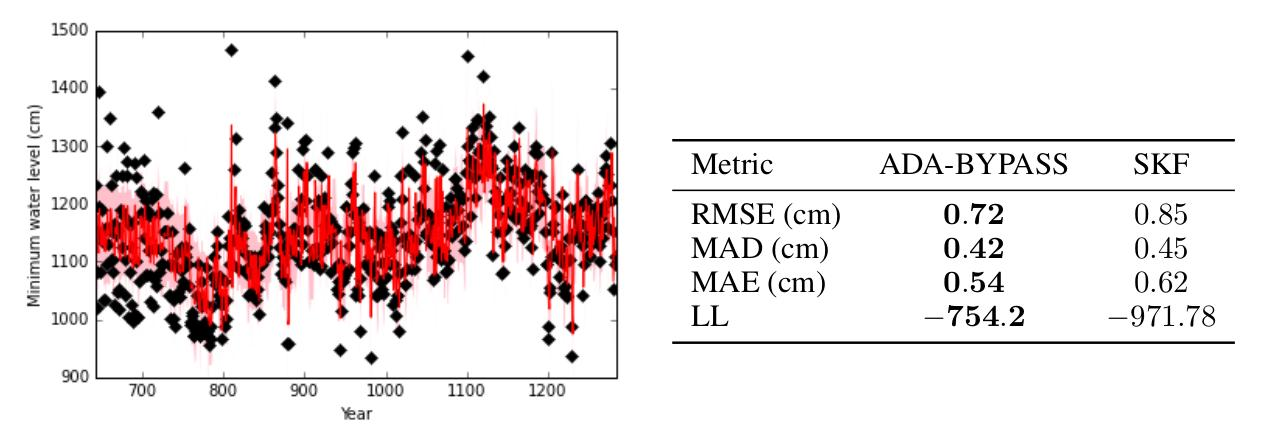
\includegraphics[width=\textwidth, keepaspectratio]{nile}
\caption{Online one-year ahead predictions for the Nile’s minimum water levels. Left panel: observed levels (black diamonds), predicted levels (red line) and ±1 standard deviation error bars
(pink area). Right panel: predictive performances; error metrics shown are root mean squared error (RMSE), mean absolute deviation (MAD), mean absolute error (MAE) and predictive log likelihood
(LL).}
\label{fig:nile}
\end{figure}

\subsubsection{Wind speed data}

To demonstrate the superior performance of ADA-BYPASS on a large data set, we next present the series of anemometer wind speed measurements (in m/s) from a Danish wind turbine. The data were sampled at ten-minute intervals for just over nine months, resulting in a total of 40,174 measurements. The ten-minute lookahead predictive performance achieved by each method is reported in Table~\ref{tab:windspeed}.
\begin{table}[t]
\caption{Predictive performance of ADA-BYPASS vs SKF on the wind speed data set.}
\label{tab:windspeed}
\centering
  \begin{tabular}{lcc}
    \toprule
    Metric    & ADA-BYPASS     & SKF \\
    \midrule
    RMSE (m/s) & \textbf{0.6}  & 0.64     \\
    MAD (m/s)     & \textbf{0.3} & 0.31      \\
    MAE (m/s)     & \textbf{0.42}       & 0.44  \\
    LL     & \textbf{-24,971.75}       & -30,140.04  \\
    \bottomrule
  \end{tabular}
\end{table}

\subsubsection{Statistical arbitrage}

LGSSMs, and variants thereof, have seen a widespread use in statistical arbitrage strategies, notably in pairs trading \citep{epchan, triantafyllopoulos11, montana09}. In this area, they serve as a dynamic model for the price spread between two assets. In our application, we seek to find the \emph{hedge ratio}\footnote{The hedge ratio of a particular asset is the number of units of that asset we should buy or sell in a portfolio. If the asset is a stock, then the number of units corresponds to the number of shares. A negative hedge ratio indicates we should sell that asset.} and the predictive standard deviation of the spread. The observable variable is thus one of the price series $y$, and the hidden variable is the hedge ratio $w$. We assume that both variables can be modelled via the following measurement and transition equations, respectively:
\begin{align}
	& y_t = w_t x_t + u_t, \qquad u_t \sim \mathcal{N}(u_t | \mu, \beta^{-1}),
	\\
	& w_t = w_{t-1} + \xi_t, \qquad \xi_t \sim \mathcal{N}(\xi_t | 0, \alpha^{-1}),
\end{align}
where $x$ is the price series of the other asset. Typically, $\alpha$, $\beta$ and $\mu$ are manually selected in hindsight \citep{epchan}. However, this practice is highly prone to the so-called \emph{data-snooping bias}: these parameters can be tweaked so as to optimise the backtesting performance of the strategy. The ADA-BYPASS algorithm automatically tunes its underlying parameters, so it does not suffer from this caveat.

We tested ADA-BYPASS on a pair of exchange-traded funds (ETFs) consisting of the SPDR gold trust GLD and the gold-miners ETF GDX. This ETF pairing is a favourite in the financial industry, because the value of gold-mining companies is very much based on the value of gold. We downloaded the corresponding, daily adjusted closing prices from Yahoo! Finance, between May 22, 2006 and April 22, 2015.

Rather than maximising profits, most investors attempt to maximise risk-adjusted returns, as advocated by modern portfolio theory. The Sharpe ratio is the most widely used measure of risk-adjusted returns \citep{sharpe}. Besides the Sharpe ratio, the maximum drawdown and maximum drawdown duration are two other popular metrics to evaluate trading strategies. From Table~\ref{tab:statarb}, we can clearly discern that ADA-BYPASS beats SKF by a significant margin in terms of the aforementioned performance metrics.
%\begin{table}[t]
%\caption{Performance of the GDX-GLD pairs trade under ADA-BYPASS and SKF.}
%\label{tab:statarb}
%\centering
%  \begin{tabular}{lcc}
%    \toprule
%    Metric    & ADA-BYPASS     & SKF \\
%    \midrule
%    Sharpe ratio & \textbf{1.12}  & 0.7     \\
%    Maximum drawdown (\%)     & \textbf{14.61} & 73.05      \\
%    Maximum drawdown duration (trading days)     & \textbf{375}       & 567  \\
%    \bottomrule
%  \end{tabular}
%\end{table}
\begin{table}[t]
\caption{Performance of the GDX-GLD pairs trade under ADA-BYPASS and SKF.}
\label{tab:statarb}
\centering
  \begin{tabular}{lcc}
    \toprule
    Metric    & ADA-BYPASS     & SKF \\
    \midrule
    Sharpe ratio & \textbf{1.00}  & 0.70     \\
    Maximum drawdown (\%)     & \textbf{15.93} & 73.05      \\
    Maximum drawdown duration (trading days)     & \textbf{404}       & 567  \\
    \bottomrule
  \end{tabular}
\end{table}

\begin{mccorrection}
\subsection{Impact of different priors}
\end{mccorrection}

In order to gauge the effects of our proposed Bayesian approach, we shall in this section check the impact of different means and standard deviations of the prior weight distributions\footnote{We shall not, however, analyse the impact of different classes of prior distributions, as that would move us too far away from the PA regression context which, as we saw from Eqs. \eqref{eq:PA-I-optpb-altform} and \eqref{eq:PA-I-optpb}, implicitly imposes a Gaussian prior over its weights.}. Since the entire focus and pillar of this thesis are financial applications, we shall just rerun the statistical arbitrage experiment from the previous section under different means for the weight prior, but keeping the variance constant at 0. The relevant metrics are presented in Table~\ref{tab:statarb2}.
\begin{table}[H]
\caption{Performance of the GDX-GLD pairs trade under ADA-BYPASS, with different prior means $\mu$ (picked arbitrarily) and constant, zero variance.}
\label{tab:statarb2}
\centering
\scalebox{0.75}{
  \begin{tabular}{lccccccc}
    \toprule
    Metric    & $\mu=-10$ & $\mu=-2$ & $\mu=-1$ & $\mu=0$ & $\mu=1$ & $\mu=2$ & $\mu=10$ \\
    \midrule
    Sharpe ratio & 1.01 & 0.98 & 0.91 & 1.00 & 0.94 & 1.06 & 1.01 \\
    Maximum drawdown (\%)     & 14.72 & 15.51 & 15.69 & 15.93 & 16.55 & 16.00 & 13.74    \\
    Maximum drawdown duration (trading days)     & 379 & 628     & 536 & 404 & 342 & 359 & 319  \\
    \bottomrule
  \end{tabular}
}
\end{table}
The table shows that, within reason, the performance of the model is not critical upon the values of the weight prior mean ($\mu$) tested. That is as we may have expected.



\section{Concluding Remarks}

In this chapter, we stated the shortcomings of online passive-aggressive (PA) algorithms and discussed ways to overcome them. In particular, we introduced generalised passive-aggressive learning which enables the use of \emph{any} loss function within the PA framework (which, as a reminder, is restricted to the hinge loss for classification and the $\epsilon$-insensitive loss for regression).

We also developed the first online Bayesian PA regression model within the state-space setting, along with a novel, online variational inference algorithm. This model is ideal for the probabilistic prediction of non-stationary and/or very large time series, in particular massive, time-varying data streams. Results on three real-world data sets show significant improvements in predictive performance over a more standard LGSSM.

\begin{mccorrection}
One of the criticisms that could be directed at our work in this section is the absence of any evidence for why our proposed online hyperparameter tuning mechanism provides benefits, if any, over the most straightforward approach one could think of, i.e. cross-validation (CV). Although it would be possible to perform cross-validation with a rolling or sliding window, one of fundamental ideologies behind the thesis was to have online algorithms for portfolio management with the \textbf{fewest} to-be-manually-tuned hyperparameters as possible (so as to avoid data-snooping bias). Going down the rolling-window CV path goes against this fundamental ideology, as it introduces another layer of hyperparameters to be manually chosen by the practitioner (in addition to those she is trying to tune in the first place), namely 1) the size of the rolling window, 2) the size of the CV leave-out sets and 3) the CV frequency (i.e., how often do you perform CV?). For these reasons, we shall not consider rolling CV in this thesis altogether.
\end{mccorrection}
\chapter{Adaptive Gradient Methods for Dynamic Online Optimisation}
\label{ch:oo}

\minitoc


In the previous chapter, we saw how online regression can be enhanced through the use of Bayesian methods. Another important subfamily of online learning that would significantly benefit from a Bayesian approach is online convex optimisation. In this area, online gradient descent (OGD) is arguably the most popular algorithm. However, OGD can often be difficult to use for practitioners, because its performance is very sensitive to the choice of learning rate parameter. In this chapter, we shall discuss how a Bayesian treatment of OGD can overcome this limitation, by providing a mechanism to infer the learning rate from the data. The resulting algorithm, named \emph{maximum posterior gradient} (MAPGRAD), also allows us to cheaply compute uncertainty estimates of the learner's actions, based on an approximate posterior distribution over these. 

In addition to the above, we shall demonstrate how the generalised passive-aggressive framework developed in the previous chapter can be adapted to the context of bandit convex optimisation. The resulting \emph{passive-aggressive convex optimisation} (PACO) method helps alleviate the difficulties in tuning the learning rate within that context.


\section{Introduction}
\label{sec:intro}

Online convex optimisation (OCO) is a fundamental tool for solving a wide variety of machine learning problems, such as online routing, ad selection for search engines and spam filtering \citep{shalev-shwartz11, oco}. It can be formulated as a repeated game between a learner and an adversary. On round $t$ of the game, the learner selects an action, i.e.\ a point $\mathbf{w}_t$ from a convex set $\Omega$, while the adversary chooses a convex loss function $f_t : \Omega \rightarrow \mathbb{R}$. Subsequently, the learner incurs a loss of $f_t(\mathbf{w}_t)$ and is provided with feedback $\phi_t(\mathbf{w}_t, f_t)$ about the loss function $f_t(\cdot)$ selected by the adversary. In this work, we shall consider the following three canonical feedback structures:
\begin{enumerate}
	\item \emph{full-information feedback}, in which the entire function $f_t(\cdot)$ is revealed to the learner after her selection of $\mathbf{w}_t$;
%	\item \emph{subgradient feedback}, meaning the learner only receives subgradient information $\mathbf{g}_t \in \partial f_t(\mathbf{w}_t)$, where $\partial f(x)$ denotes the subdifferential set of a function $f(\cdot)$ evaluated at $x$ (see Definition~\ref{def:subgradient});
\begin{mccorrection}
	\item \emph{gradient feedback}, meaning the learner only receives gradient information $\mathbf{g}_t \equiv \nabla f_t(\mathbf{w}_t)$, i.e. the gradient of the loss function $f_t(\cdot)$ evaluated at the weight vector $\mathbf{w}_t$;
\end{mccorrection}
	\item \emph{bandit feedback}, characterised by the revelation of the incurred loss $f_t(\mathbf{w}_t)$ only.
\end{enumerate}
An outline of the OCO problem under these feedback scenarios is given in Algorithm~\ref{alg:oco}.
\begin{algorithm}[H]
  \caption{Online Convex Optimisation}
  \label{alg:oco}
  \begin{algorithmic}[1]
    \STATE {\bfseries Input:} a convex set $\Omega$
    \FOR{$t=1, 2, \ldots$}
      \STATE the learner chooses a vector $\mathbf{w}_t \in \Omega$
      \STATE the adversary selects a loss function $f_t : \Omega \rightarrow \mathbb{R}$
      \STATE the learner incurs a loss of $f_t(\mathbf{w}_{t})$ and observes
      \begin{itemize}
		\item the loss function $f_t(\cdot)$ in the full-information setting
%		\item the subgradient $\mathbf{g}_t \in \partial f_t(\mathbf{w}_t)$ in the subgradient-feedback setting
\begin{mccorrection}
		\item the gradient $\mathbf{g}_t \equiv \nabla f_t(\mathbf{w}_t)$ in the gradient-feedback setting
\end{mccorrection}
		\item the loss value $f_t(\mathbf{w}_t)$ in the bandit-feedback setting
	\end{itemize}
    \ENDFOR
  \end{algorithmic}
\end{algorithm}

The standard performance measure for OCO problems is the so-called \emph{regret}, which is defined as the difference between the learner's cumulative loss and that of a relatively weak benchmark, namely the single best action in hindsight, or a \emph{static clairvoyant}:
\begin{equation}
\label{eq:static-regret}
	\sum_{t=1}^T f_t(\mathbf{w}_t) \, - \, \min_{\mathbf{w} \in \Omega} \, \sum_{t=1}^T f_t(\mathbf{w}).
\end{equation}
Over the past decades, various online algorithms have been proposed to yield sublinear regret under a variety of feedback structures, with a focus on a class of either convex or strongly convex loss functions.
%The original work of \citet{zinkevich03} considered the class of convex functions and focused on the case of full-information feedback, providing an \emph{online gradient descent} (OGD) algorithm with regret of order $\sqrt{T}$. \citet{hazan07} achieve regret of order $\log T$ for a class of strongly convex loss functions when the subgradient of $f_t(\cdot)$, evaluated at $\mathbf{w}_t$, is observed. Additional algorithms were shown to be rate-optimal under further assumptions on the function class (see, e.g., \citep{kalai05, hazan07}), or other feedback structures such as multipoint access \citep{agarwal10}.
\begin{mccorrection}
The original work of \citet{zinkevich03} considered the class of convex functions and focused on the case of full-information feedback, providing an \emph{online gradient descent} (OGD) algorithm with regret of order $\sqrt{T}$. \citet{hazan07} achieve regret of order $\log T$ for a class of strongly convex loss functions when the gradient of $f_t(\cdot)$, evaluated at $\mathbf{w}_t$, is observed. Additional algorithms were shown to be rate-optimal under further assumptions on the function class (see, e.g., \citep{kalai05, hazan07}), or other feedback structures such as multipoint access \citep{agarwal10}.
\end{mccorrection}

Though equipped with rich theories, the notion of regret fails to illustrate the performance of online algorithms in a dynamic setting, as a \emph{static} comparator is used in Eq. \eqref{eq:static-regret}. To overcome this limitation, there has been a recent surge of interest in analysing a more stringent metric, namely \emph{dynamic regret} \citep{hall&willett13, hall&willett15, jadbabaie15, besbes15, mokhtari16, yang16, zhang17, gao18}, in which the cumulative loss of the learner is compared against that attained by a sequence $\mathbf{w}_{1:T}^* \equiv \mathbf{w}_1^*, \mathbf{w}_2^*, \ldots, \mathbf{w}_T^*$ of instantaneous-loss minimisers, i.e.\
\begin{equation}
\label{eq:dynamic-regret}
  \textbf{Reg}_T^d
%  \equiv \textbf{Reg}_T^d(\mathbf{w}_{1:T}^*)
  \equiv \sum_{t=1}^T f_t(\mathbf{w}_t) \, - \, \sum_{t=1}^T f_t(\mathbf{w}_t^*)
  = \sum_{t=1}^T f_t(\mathbf{w}_t) \, - \, \sum_{t=1}^T \min_{\mathbf{w} \in \Omega} \, f_t(\mathbf{w}),
\end{equation}
where $\mathbf{w}^*_t \in \argmin_{\mathbf{w} \in \Omega} \, f_t(\mathbf{w})$.
In other words, Eq. \eqref{eq:dynamic-regret} measures the quality of an algorithm, and the sequence $\mathbf{w}_{1:T}$ of actions it generates, by comparing its performance to a \emph{dynamic clairvoyant} who knows the sequence of loss functions in advance, and hence selects the minimiser $\mathbf{w}_t^*$ at each step.
%Compared to traditional regret in Eq. \eqref{eq:static-regret} (also termed \emph{static regret}), dynamic regret is more aggressive since the dynamic clairvoyant can never do worse than her static counterpart, by virtue of the following property:
%\begin{equation}
%	\sum_{t=1}^T \min_{\mathbf{w} \in \Omega} \, f_t(\mathbf{w})
%	\, \leq \, \min_{\mathbf{w} \in \Omega} \, \sum_{t=1}^T f_t(\mathbf{w}).
%\end{equation}

\begin{mccorrection}
Compared to traditional regret in Eq. \eqref{eq:static-regret} (also termed \emph{static regret}), dynamic regret is more aggressive in the sense that
\begin{equation}
	\min_{\mathbf{w} \in \Omega} \, \sum_{t=1}^T f_t(\mathbf{w})
	\, \geq \, \sum_{t=1}^T \min_{\mathbf{w} \in \Omega} \, f_t(\mathbf{w}),
\end{equation}
which is a consequence of the fact that the maximum of a sum is at most the sum of maxima (see, e.g., \url{https://math.stackexchange.com/questions/
740074/maximum-of-sum-is-at-most-the-sum-of-maxima}).
As the next example from \citep{besbes15} shows, the dynamic clairvoyant used as benchmark in Eq. \eqref{eq:dynamic-regret} can be a significantly harder target than the single best action defining the static clairvoyant in Eq. \eqref{eq:static-regret}.
\begin{example}
Assume an action set $\Omega = [-1, 2]$. % and variation budget $V_T = 1$. Set
Set
\begin{equation}
	f_{t}(w) = 
	\begin{cases}
		w^2 & \text{if } t \leq T/2 \\
		w^2 - 2w & \text{otherwise}
	\end{cases}
\end{equation}
for any $w \in \Omega$. Then, the single best action is suboptimal at each step, and
\begin{equation}
	\min_{w\in\Omega} \sum_{t=1}^T f_t(w) - \sum_{t=1}^T \min_{w \in \Omega} \, f_t(w) = \frac{T}{4}.
\end{equation}
\end{example}
Hence, algorithms that achieve performance that is `close' to the static clairvoyant in the static OCO setting may perform quite poorly in the dynamic OCO setting (in particular, they may, as the example above suggests, incur linear regret in that setting). These algorithms include, but are in no way limited to, the seminal online gradient descent (OGD) algorithm with a learning-rate schedule of $\eta_t = 1/\sqrt{t}$ \citep{zinkevich03}. Therefore, we shall refrain from comparing the impact of the methods introduced in this chapter to that schedule on (dynamic) regret. Nevertheless, for the avid reader, in Section~\ref{sec:adapamr-eval} we compare the empirical performance of Zinkevich's OGD algorithm against that of the proposed methods in this thesis.
\end{mccorrection}
%The other clear implication is that any algorithm achieving sublinear dynamic regret will necessarily also have sublinear static regret (note however that the converse is not generally true). For this reason, we shall restrict our attention to what we call \emph{dynamic OCO}, that is online convex optimisation for which dynamic, rather than static, regret is the performance metric.

As in the case of static OCO --- i.e., online convex optimisation under static regret --- the OGD method has established itself as the candidate of choice for solving dynamic OCO problems, as demonstrated by its widespread use in the literature \citep{besbes15, mokhtari16, yang16, zhang17, gao18}.
However, OGD can often be frustrating to use for practitioners, because its performance is very sensitive to the choice of the learning rate parameter. While previous work in the dynamic OCO literature has proposed various ways to select the learning rate, these are based on theoretical considerations as to which assumptions of smoothness, convexity and temporal variation in the loss-function sequence are required to minimise the corresponding regret bounds, in some cases even causing the OGD algorithm to become unfeasible without the benefit of hindsight.

To overcome this practical hurdle, we develop in this chapter two novel adaptation techniques for tuning the learning rate parameter in an \emph{online} and \emph{data-dependent} fashion. Specifically, we propose the following algorithms:
\begin{itemize}
	\item \emph{Maximum Posterior Gradient} (MAPGRAD), in which we interpret OGD as a Bayesian hierarchical model, treat the learning rate as a \emph{nuisance parameter} and marginalise it, and set the weight vector equal to its \emph{maximum a posteriori} (MAP) value under the resulting marginal weight posterior;
	\item \emph{Passive-Aggressive Convex Optimisation} (PACO), a generalisation of online passive-aggressive (PA) learning \citep{crammer06} to general loss functions and feasibility regions other than $\mathbb{R}^n$, allowing this framework to be applied successfully to a dynamic OCO setting.
\end{itemize}
%Since it requires knowledge of the loss $f_t(\mathbf{w}_t)$ incurred by the learner at each stage $t$, the PACO algorithm can only be used in the full-information and bandit settings. As for MAPGRAD, it is applicable under both the full-information and subgradient feedback structures.
\begin{mccorrection}
Since it requires knowledge of the loss $f_t(\mathbf{w}_t)$ incurred by the learner at each stage $t$, the PACO algorithm can only be used in the full-information and bandit settings. As for MAPGRAD, it is applicable under both the full-information and gradient feedback structures. Additionally, wherever needed, we shall assume that the loss functions are differentiable.
\end{mccorrection}

To the best of our knowledge, this is pioneering work as far as the dynamic OCO literature is concerned. Granted, beyond this literature, there has been a rich line of work on adaptive learning rate methods over the past few years\footnote{This continues to be an active area of research at the time of writing, especially in the deep learning community.} and, in the next section, we briefly review those that are somehow related to our work. However, we are not aware of any techniques that have approached the automatic tuning of the learning rate from a Bayesian angle, making our MAPGRAD algorithm one of a kind.


\section{Related Work}
\label{sec:related-work}

The closest papers to our work, at least in spirit, are \citep{badam}, \citep{probabilistic-ipm} and \citep{blondel14}. Below we discuss the similarities, and differences, between their work and ours. Other prominent, albeit unrelated, adaptive learning rate methods include ADAGRAD \citep{adagrad} and exponential-moving-average variants thereof, namely RMSPROP \citep{rmsprop}, ADADELTA \citep{adadelta} and ADAM \citep{adam}.

\paragraph{\citep{badam}}

In the spirit of MAPGRAD, \citet{badam} have recently introduced a framework to cheaply build Bayesian neural networks from adaptive learning rate methods such as ADAGRAD and ADAM. Like ours, this framework is also based on a novel probabilistic interpretation of a generic update rule encompassing any adaptive gradient-based scheme, and as such is an elegant generalisation of MAPGRAD. Nevertheless, since the focus of their paper is on obtaining cheap uncertainty estimates for neural-network weights, \citet{badam} fail to discuss how to leverage their Bayesian approach to infer the learning rate parameter from the data.

\paragraph{\citep{probabilistic-ipm}}

This is another interesting paper that bears much resemblance to our MAPGRAD framework. The authors highlight a connection between the incremental proximal method (IPM) --- to which online gradient descent provides a first-order approximation, as we shall see later --- and stochastic filters. This connection is obtained as the result of a probabilistic interpretation of IPM. Interestingly, the authors demonstrate that in the case of linear regression, the probabilistic variant of IPM can be viewed as a Kalman filter. By analogy, for non-linear regressors, there is a direct correspondence between probabilistic IPM and the extended Kalman filter. Note however that, unlike MAPGRAD, the goal of the Bayesian treatment in \citep{probabilistic-ipm} is not to derive an adaptation mechanism for tuning the learning rate parameter. 

\paragraph{\citep{blondel14}}

An adaptive learning rate method that is closely related to our PACO algorithm is NN-PA, which was introduced in \citep{blondel14}. Like PACO, NN-PA is a variant of online passive-aggressive learning that was proposed as a way of overcoming the learning-rate sensitivity of stochastic gradient descent in the particular field of non-negative matrix factorisation. In fact, NN-PA is a special case of PACO in which $\Omega = \mathbb{R}^n_+$ and the loss function is given by the $\epsilon$-insensitive loss function, which is the loss used in the original PA framework of \citet{crammer06}.


\section{Problem Formulation}

Having already laid out the key building blocks and ideas behind our problem formulation in Section~\ref{sec:intro}, the purpose of the present section is to fill in any gaps and make that exposition more precise where needed. Some repetition is expected but is kept to a minimum.

%A dynamic OCO problem consists of a convex set $\Omega \subseteq \mathbb{R}^n$ and an a priori unknown sequence $\{f_t(\cdot)\}_{t \geq 1} \subset \mathcal{F}$, where $\mathcal{F}$ represents a class of sequences of convex loss functions from $\Omega$ onto $\mathbb{R}$. At any stage $t$, the decision maker selects a point $\mathbf{w}_t \in \Omega$, and then observes some feedback $\phi_t$. As we mentioned earlier, we shall confine ourselves to the full-information, subgradient and bandit feedback structures, in which $\phi_t = f_t$, $\phi_t = \mathbf{g}_t \in \partial f_t(\mathbf{w}_t)$ and $\phi_t = f_t(\mathbf{w}_t)$, respectively, for each step $t$.
\begin{mccorrection}
A dynamic OCO problem consists of a convex set $\Omega \subseteq \mathbb{R}^n$ and an a priori unknown sequence $\{f_t(\cdot)\}_{t \geq 1} \subset \mathcal{F}$, where $\mathcal{F}$ represents a class of sequences of convex loss functions from $\Omega$ onto $\mathbb{R}$. At any stage $t$, the decision maker selects a point $\mathbf{w}_t \in \Omega$, and then observes some feedback $\phi_t$. As we mentioned earlier, we shall confine ourselves to the full-information, gradient and bandit feedback structures, in which $\phi_t = f_t$, $\phi_t = \mathbf{g}_t \equiv \nabla f_t(\mathbf{w}_t)$ and $\phi_t = f_t(\mathbf{w}_t)$, respectively, for each step $t$.
\end{mccorrection}

The efficacy of an algorithm --- that is, a strategy for choosing a sequence of decisions $\mathbf{w}_t \in \Omega$ --- is measured relative to a fictitious clairvoyant who knows the function sequence $\{f_t(\cdot)\}_{t \geq 1}$ in advance, and therefore is able to select, on each round $t$, a point $\mathbf{w}_t^*$ such that $\mathbf{w}_t^* \in \argmin_{\mathbf{w} \in \Omega} \, f_t(\mathbf{w})$. The goal of the learner is to mimic the behaviour of the clairvoyant as closely as possible, that is to say, to find an algorithm whose efficacy is as similar as possible to that of the algorithm the clairvoyant would deploy. This corresponds to playing the strategy with the lowest possible dynamic regret, as defined in Eq. \eqref{eq:dynamic-regret}. Ideally, therefore, the learner would like to play the minimiser $\mathbf{w}_t^*$ of $f_t(\cdot)$ at each time step $t$, since this strategy would yield zero dynamic regret. This is not possible, however, so a surrogate function must be used in place of $f_t(\cdot)$. Loosely speaking, it would make sense to approximate the unobserved $f_t(\cdot)$ with the most recent loss function $f_{t-1}(\cdot)$ whenever the minimum of the latter is sufficiently close to that of the former:
\begin{equation}
\label{eq:oco-val-fct-approx}
	\min_{\mathbf{w}\in\Omega} \; f_{t-1}(\mathbf{w})
	\, \approx \, \min_{\mathbf{w}\in\Omega} \; f_t(\mathbf{w}).
\end{equation}

To ascertain the conditions under which the approximation in Eq. \eqref{eq:oco-val-fct-approx} is valid, consider the change in the minimal loss from time step $t-1$ to time step $t$, which is defined by
\begin{equation}
\label{eq:minimal-loss-delta}
	\Delta f_t^*
	\equiv \min_{\mathbf{w}\in\Omega} \; f_t(\mathbf{w}) - \min_{\mathbf{w}\in\Omega} \; f_{t-1}(\mathbf{w}),
	\qquad t = 2, 3, \ldots, T.
\end{equation}
Using the standard properties of infima and suprema, we can write
\begin{equation}
\label{eq:minimal-loss-delta-prop}
	|\Delta f_t^*|
	\leq \max_{\mathbf{w}\in\Omega} \; |f_t(\mathbf{w}) - f_{t-1}(\mathbf{w})|,
	\qquad t = 2, 3, \ldots, T.
\end{equation}
Summing both sides over $t$, we obtain
\begin{equation}
\label{eq:variation-functional-constraint}
	\sum_{t=2}^{T} |\Delta f_t^*|
	\leq \mathrm{Var}(f_1, \ldots, f_T)
	\equiv \sum_{t=2}^{T} \max_{\mathbf{w}\in\Omega} \; |f_t(\mathbf{w}) - f_{t-1}(\mathbf{w})|.
\end{equation}
%where the variation functional $\mathrm{Var}(\cdot)$ is defined as
%\begin{equation}
%	\mathrm{Var}(f_1, \ldots, f_T) \equiv \sum_{t=1}^{T-1} \max_{\mathbf{w}\in\Omega} \; |f_{t+1}(\mathbf{w}) - f_t(\mathbf{w})|.
%\end{equation}
Roughly speaking, the variation functional $\mathrm{Var}(\cdot)$ measures the extent to which functions can change from one time step to the next, and adds this up over the horizon $T$.
By virtue of Eq. \eqref{eq:variation-functional-constraint}, Eq. \eqref{eq:oco-val-fct-approx} is satisfied when the variation functional is bounded above, that is to say when there exists a scalar $V_T$ such that
\begin{equation}
	\mathrm{Var}(f_1, \ldots, f_T) \leq V_T.
\end{equation}
We refer to $V_T$ as the \emph{variation budget} over $\mathcal{F}$. Note that this quantity is allowed to depend on the length of the horizon, and therefore measures the variation scale relative to the latter. In light of all the aforementioned considerations, we shall further constrain the set of admissible loss-function sequences as follows.
\begin{assumption}
\label{ass:functional-variation}
The sequence of loss functions $f_{1:T}$ belong to the \emph{temporal uncertainty set} $\mathcal{V}$, defined by
\begin{equation}
\label{eq:temporal-uncertainty-set}
	\mathcal{V}
	\equiv \Big\{f_{1:T} \subset \mathcal{F} \; \Big| \; \sum_{t=1}^{T-1} \max_{\mathbf{w}\in\Omega} \; |f_{t+1}(\mathbf{w}) - f_t(\mathbf{w})| \leq V_T\Big\},
\end{equation}
where $\{V_t\}_{t=1, 2, \ldots}$ is a non-decreasing sequence of scalars such that $V_t \leq t$ for all $t$, with $V_1 = 0$ and $V_2 \geq 1$ for normalisation purposes.
\end{assumption}
\begin{mccorrection}
It is worthwhile noting that the sequence $\{V_t\}_{t=1, 2, \ldots}$ is allowed to grow linearly. While this may seem odd at first, \citep[Proposition~1]{besbes15} shows that if the variation budget is \emph{linear} in $T$, then, as one may expect, it is \emph{impossible} to achieve sublinear dynamic regret. Conversely, if $V_T$ is \emph{sublinear} in $T$, then algorithms that achieve sublinear dynamic regret \emph{do exist}. With that in mind, hereon, we will focus on the case in which the variation budget is sublinear in $T$.
\end{mccorrection}
Even though the variation budget places some restrictions on the possible evolution of loss functions, it still allows for many different temporal patterns, including continuous change, discrete shocks and a non-constant rate of change (see \citep{besbes15} for examples and illustrations of such variation instances). More importantly for our purposes, these restrictions justify the following action choices:
\begin{equation}
\label{eq:action-choices}
	\mathbf{w}_{t+1} \in \argmin_{\mathbf{w}\in\Omega}\; f_t(\mathbf{w}), \qquad t = 1, 2, \ldots,
\end{equation}
with an arbitrary initial action $\mathbf{w}_1\in\Omega$.

Before discussing how to implement strategy \eqref{eq:action-choices} within the different feedback structures considered in this chapter, it is worth emphasising the implications of the temporal uncertainty set \eqref{eq:temporal-uncertainty-set} for dynamic regret.

\subsection{Temporal variation and dynamic regret}

In addition to allowing the learner to mimic the clairvoyant strategy in a fairly accurate way, the temporal uncertainty set ensures the existence of algorithms with sublinear dynamic regret rates. This is the primary reason why it was introduced in \citep{besbes15}.

Indeed, in the absence of restrictions on the variation in the adversary's choices, it would not be possible to achieve sublinear dynamic regret, because drastic fluctuations would render the problem intractable. For instance, \citet{besbes15} proved that if there is no restriction on the variation of loss functions, then the dynamic regret is linear in $T$, regardless of the strategy adopted by the learner. Let us illustrate this with a contrived example.
\begin{example}
Suppose that for $t \in [T]$, after the learner has picked an action $w_t \in \mathbb{R}$, the adversary randomly chooses the loss function among $f_t(w) = (w - 1)^2$ and $f_t(w) = (w + 1)^2$. The expected instantaneous regret for round $t$ in this example satisfies
\begin{equation}
\begin{split}
	\mathbb{E}[f_t(w_t) - f_t(w_t^*)]
	&= \frac{1}{2}\left[(w_t - 1)^2 - \min_{w}\, (w - 1)^2\right] + \frac{1}{2}\left[(w _t + 1)^2 - \min_{w}\, (w + 1)^2\right]
	\\	
	&= \frac{1}{2}(w_t - 1)^2 + \frac{1}{2}(w_t + 1)^2	
	= w_t^2 + 1
	\geq 1,
\end{split}
\end{equation}
whence $\mathbb{E}(\emph{\textbf{Reg}}_T^d) = \sum_{t=1}^T (w_t^2 + 1) \geq T$.
\end{example}


\section{Full Information}

In this section, we assume that on each round, the entire loss function is available to the learner after she makes her decision. Specifically, at each stage $t$, the sequence of events is as follows:
\begin{enumerate}
	\item the learner submits an action $\mathbf{w}_t \in \Omega$;
	\item the adversary chooses a loss function $f_t(\cdot)$ and reveals it to the learner;
	\item the learner incurs a (known) loss of $f_t(\mathbf{w}_t)$.
\end{enumerate}
As discussed in the previous section, the optimal strategy for the learner is to start with an arbitrary choice $\mathbf{w}_1 \in \Omega$, followed by choices $\mathbf{w}_{t+1}$ ($t \geq 1$) such that
\begin{equation}
\label{eq:action-choices-2}
	\mathbf{w}_{t+1} \in \argmin_{\mathbf{w} \in \Omega} \, f_t(\mathbf{w}).
\end{equation}
In the best case scenario, we are able to analytically solve the optimisation problem in Eq. \eqref{eq:action-choices-2}. In this case, it is relatively straightforward to show that the dynamic regret associated with the action choices in Eq. \eqref{eq:action-choices-2} has an upper bound on the order of the variation in the sequence of loss functions. This is formally stated in Proposition~\ref{prop:action-choices-dynamic-regret}.
\begin{mccorrection}
\begin{proposition}
\label{prop:action-choices-dynamic-regret}
Under the conditions set out in Assumption~\ref{ass:functional-variation}, with the exception that $V_t < t$ (rather than $V_t \leq t$) for all $t$, the action sequence
\begin{equation}
	\mathbf{w}_{t+1} \in \argmin_{\mathbf{w}\in\Omega}\; f_t(\mathbf{w}), \qquad t \in [T-1],
\end{equation}
with $\mathbf{w}_1$ being an arbitrary element of $\Omega$, achieves the following dynamic regret bound:
\begin{equation}
	\sum_{t=1}^T f_t(\mathbf{w}_t) - \sum_{t=1}^T f_t(\mathbf{w}_t^*) \leq [f_1(\mathbf{w}_1) - f_1(\mathbf{w}_1^*)] + 2V_T.
\end{equation}
\end{proposition}
\end{mccorrection}
\begin{proof}
For each $t \in [T-1]$ and each $\mathbf{w}_t^* \in \argmin_{\mathbf{w}\in\Omega}\; f_t(\mathbf{w})$, we can write
\begin{align}
	f_{t+1}(\mathbf{w}_{t+1}) - f_{t+1}(\mathbf{w}_{t+1}^*)
	&= f_{t+1}(\mathbf{w}_t^*) - f_{t+1}(\mathbf{w}_{t+1}^*)
	\nonumber \\
	&= [f_{t+1}(\mathbf{w}_t^*) - f_t(\mathbf{w}_t^*)] + [f_t(\mathbf{w}_t^*) - f_{t+1}(\mathbf{w}_{t+1}^*)]
	\nonumber \\	
	&\leq |f_{t+1}(\mathbf{w}_t^*) - f_t(\mathbf{w}_t^*)| + |\Delta f_{t+1}^*|
	\nonumber \\
	&\leq |f_{t+1}(\mathbf{w}_t^*) - f_t(\mathbf{w}_t^*)| + \max_{\mathbf{w}\in\Omega} \; |f_{t+1}(\mathbf{w}) - f_t(\mathbf{w})|,
	\label{eq:action-choices-dynamic-regret-proof-1}
\end{align}
where we have used the definition \eqref{eq:minimal-loss-delta} in the first inequality, while the second inequality is a direct consequence of property \eqref{eq:minimal-loss-delta-prop}.

By definition, the following inequality holds for any $\mathbf{w}\in\Omega$:
\begin{equation}
	|f_{t+1}(\mathbf{w}) - f_t(\mathbf{w})|
	\leq \max_{\mathbf{w}\in\Omega} \; |f_{t+1}(\mathbf{w}) - f_t(\mathbf{w})|.
\end{equation}
Setting $\mathbf{w} = \mathbf{w}_t^*$ and plugging the resulting inequality into Eq. \eqref{eq:action-choices-dynamic-regret-proof-1} yields
\begin{equation}
	f_{t+1}(\mathbf{w}_{t+1}) - f_{t+1}(\mathbf{w}_{t+1}^*) \leq 2\max_{\mathbf{w}\in\Omega} \; |f_{t+1}(\mathbf{w}) - f_t(\mathbf{w})|.
\end{equation}
Summing both sides over $t$ and using Assumption~\ref{ass:functional-variation}, we obtain
\begin{equation}
	\sum_{t=1}^{T-1}[f_{t+1}(\mathbf{w}_{t+1}) - f_{t+1}(\mathbf{w}_{t+1}^*)]
	\leq 2\sum_{t=1}^{T-1}\max_{\mathbf{w}\in\Omega} \; |f_{t+1}(\mathbf{w}) - f_t(\mathbf{w})|
	\leq 2V_T.
\end{equation}
It immediately follows that
\begin{equation}
\begin{split}
	\sum_{t=1}^{T}[f_t(\mathbf{w}_t) - f_t(\mathbf{w}_t^*)]
%	&= [f_1(\mathbf{w}_1) - f_1(\mathbf{w}_1^*)]
%	+ \sum_{t=2}^{T}[f_t(\mathbf{w}_t) - f_t(\mathbf{w}_t^*)]
%	\\
	&= [f_1(\mathbf{w}_1) - f_1(\mathbf{w}_1^*)]
	+ \sum_{t=1}^{T-1}[f_{t+1}(\mathbf{w}_{t+1}) - f_{t+1}(\mathbf{w}_{t+1}^*)]
	\\
	&\leq [f_1(\mathbf{w}_1) - f_1(\mathbf{w}_1^*)]
	+ 2V_T,
\end{split}
\end{equation}
which completes the proof.
\end{proof}

%In most cases, however, the optima in Eq. \eqref{eq:action-choices-2} cannot be found by algebraic means alone, and numerical techniques are required. While there are numerous such techniques that proceed iteratively towards the optimum, including line-search, trust-region, conjugate-gradients and quasi-Newton methods, we shall only discuss gradient/subgradient descent here, as it forms the basis for all of the algorithms that we shall develop in this chapter. For a detailed discussion of alternative methods, we refer the reader to \citep{nocedal}.
\begin{mccorrection}
In most cases, however, the optima in Eq. \eqref{eq:action-choices-2} cannot be found by algebraic means alone, and numerical techniques are required. While there are numerous such techniques that proceed iteratively towards the optimum, including line-search, trust-region, conjugate-gradients and quasi-Newton methods, we shall only discuss gradient descent here, as it forms the basis for all of the algorithms that we shall develop in this chapter. For a detailed discussion of alternative methods, we refer the reader to \citep{nocedal}.
\end{mccorrection}

%\subsection{Subgradient descent}
\subsection{Gradient descent}

%Subgradient descent is the simplest and oldest of optimisation methods. It is an \emph{iterative} procedure in the sense that it proceeds in iterations, each seeking to decrease the value of the objective function. The method is based on the following principle: locally, if we are at a point $\mathbf{v}_{t}^{(k)} \in \Omega$, we can decrease $f_t(\cdot)$ by taking a step in the direction $-\mathbf{g}_t^{(k)}$, where $\mathbf{g}_t^{(k)}$ is a subgradient of $f_t(\cdot)$ evaluated at $\mathbf{v}_{t}^{(k)}$, i.e.\ $\mathbf{g}_t^{(k)} \in \partial f_t(\mathbf{v}_{t}^{(k)})$. Mathematically, this idea is expressed by means of the update rule
%\begin{equation}
%	\mathbf{v}_{t}^{(k+1)}
%	= \Pi_{\Omega}(\mathbf{v}_{t}^{(k)} - \eta\mathbf{g}_t^{(k)}),
%	\qquad k \in [K],
%\end{equation}
%for some fixed learning rate $\eta > 0$ and an integer $K \geq 1$ representing the number of iterations until convergence is achieved.
\begin{mccorrection}
Gradient descent is the simplest and oldest of optimisation methods. It is an \emph{iterative} procedure in the sense that it proceeds in iterations, each seeking to decrease the value of the objective function. The method is based on the following principle: locally, if we are at a point $\mathbf{v}_{t}^{(k)} \in \Omega$, we can decrease $f_t(\cdot)$ by taking a step in the direction $-\mathbf{g}_t^{(k)}$, where $\mathbf{g}_t^{(k)}$ is the gradient of $f_t(\cdot)$ evaluated at $\mathbf{v}_{t}^{(k)}$, i.e.\ $\mathbf{g}_t^{(k)} \equiv \nabla f_t(\mathbf{v}_{t}^{(k)})$. Mathematically, this idea is expressed by means of the update rule
\begin{equation}
	\mathbf{v}_{t}^{(k+1)}
	= \Pi_{\Omega}(\mathbf{v}_{t}^{(k)} - \eta\mathbf{g}_t^{(k)}),
	\qquad k \in [K],
\end{equation}
for some fixed learning rate $\eta > 0$ and an integer $K \geq 1$ representing the number of iterations until convergence is achieved.
\end{mccorrection}

%To see why subgradient descent works, assume $\Omega = \mathbb{R}^n$ and apply Taylor's theorem to expand $f_t(\mathbf{v}_{t}^{(k+1)})$ around $\mathbf{v}_{t}^{(k)}$, which for small $\eta$ yields
%\begin{equation}
%	f_t(\mathbf{v}_{t}^{(k+1)})
%	= f_t(\mathbf{v}_{t}^{(k)} - \eta\mathbf{g}_t^{(k)})
%	\approx f_t(\mathbf{v}_{t}^{(k)}) - \underbrace{\eta\Vert\mathbf{g}_t^{(k)}\Vert_2^2}_{> \, 0}
%	< f_t(\mathbf{v}_{t}^{(k)}),
%\end{equation}
%meaning the value of $f_t(\cdot)$ has decreased by moving from the old iterate $\mathbf{v}_{t}^{(k)}$ to the new one $\mathbf{v}_{t}^{(k+1)}$. If $\eta$ is non-infinitesimal, it is always possible that we will overshoot the true minimum. Making $\eta$ very small guards against this, but means that the optimisation process will take a very long time to reach a minimum.
\begin{mccorrection}
To see why gradient descent works, assume $\Omega = \mathbb{R}^n$ and apply Taylor's theorem to expand $f_t(\mathbf{v}_{t}^{(k+1)})$ around $\mathbf{v}_{t}^{(k)}$, which for small $\eta$ yields
\begin{equation}
	f_t(\mathbf{v}_{t}^{(k+1)})
	= f_t(\mathbf{v}_{t}^{(k)} - \eta\mathbf{g}_t^{(k)})
	\approx f_t(\mathbf{v}_{t}^{(k)}) - \underbrace{\eta\Vert\mathbf{g}_t^{(k)}\Vert_2^2}_{> \, 0}
	< f_t(\mathbf{v}_{t}^{(k)}),
\end{equation}
meaning the value of $f_t(\cdot)$ has decreased by moving from the old iterate $\mathbf{v}_{t}^{(k)}$ to the new one $\mathbf{v}_{t}^{(k+1)}$. If $\eta$ is non-infinitesimal, it is always possible that we will overshoot the true minimum. Making $\eta$ very small guards against this, but means that the optimisation process will take a very long time to reach a minimum.
\end{mccorrection}

%The subgradient descent algorithm adapted to the problem of dynamic OCO in a full-information setting is presented in Algorithm~\ref{alg:omgd}. It is worthwhile noting that the same algorithm has been independently proposed by \citet{zhang17}, under the name `online multiple gradient descent'. We refer the interested reader to the detailed regret analysis provided therein.
\begin{mccorrection}
The gradient descent algorithm adapted to the problem of dynamic OCO in a full-information setting is presented in Algorithm~\ref{alg:omgd}. It is worthwhile noting that the same algorithm has been independently proposed by \citet{zhang17}, under the name `online multiple gradient descent'. We refer the interested reader to the detailed regret analysis provided therein.
\begin{algorithm}[H]
%\caption{Subgradient Descent for Dynamic Online Convex Optimisation}
\caption{Gradient Descent for Dynamic Online Convex Optimisation}
\label{alg:omgd}
\begin{algorithmic}[1]
	\STATE {\bfseries Input:} convex action space $\Omega \subseteq \mathbb{R}^n$, learning rate $\eta > 0$, tolerance $\epsilon > 0$
	\STATE {\bfseries Initialisation:} arbitrary initial action $\mathbf{w}_1 \in \Omega$, $k = 1$
	\FOR{$t=1, 2, \ldots$}
		\STATE play $\mathbf{w}_t$ and receive loss function $f_t : \Omega \rightarrow \mathbb{R}$
		\STATE set $\mathbf{v}_t^{(1)} = \mathbf{w}_t$
		\STATE {\bfseries repeat}
			\begin{align*}
				\mathbf{v}_t^{(k+1)}
				&= \Pi_{\Omega}(\mathbf{v}_t^{(k)} - \eta\mathbf{g}_t^{(k)}),
%				\qquad \mathbf{g}_t^{(k)} \in \partial f_t(\mathbf{v}_t^{(k)})
				\qquad \mathbf{g}_t^{(k)} \equiv \nabla f_t(\mathbf{v}_t^{(k)})
				\\
				k &= k + 1
			\end{align*}
%		\STATE {\bfseries until} $\Vert f_t(\mathbf{v}_t^{(k+1)})\Vert_2^2 \leq \epsilon$
		\STATE {\bfseries until} $|f_t(\mathbf{v}_t^{(k+1)})| \leq \epsilon$
		\STATE obtain next action as $\mathbf{w}_{t+1} = \mathbf{v}_t^{(K)}$
	\ENDFOR
\end{algorithmic}
\end{algorithm}
Since the inner update rule in Algorithm~\ref{alg:omgd} has the form of \emph{offline} gradient descent, and in this chapter we only care about \emph{online} gradient descent, we will refrain from discussing Bayesian inference-based tools to automatically adjust the learning rate in Algorithm~\ref{alg:omgd}. In practice, one uses iteration-dependent learning rates $\eta_k$, chosen via line-search methods \citep{nocedal}.
\end{mccorrection}
%Since the inner update rule in Algorithm~\ref{alg:omgd} has the form of \emph{offline} subgradient descent, and in this chapter we only care about \emph{online} subgradient descent, we will refrain from discussing Bayesian inference-based tools to automatically adjust the learning rate in Algorithm~\ref{alg:omgd}. In practice, one uses iteration-dependent learning rates $\eta_k$, chosen via line-search methods \citep{nocedal}. 


%\section{Subgradient Feedback}
\section{Gradient Feedback}

%Full information may not be available. In general, only some partial information about the loss functions $f_t(\cdot)$ is available. In this section, we assume that the subgradient value $\mathbf{g}_t \in \partial f_t(\mathbf{w}_t)$ is the only feedback that the adversary provides to the learner at each stage $t$ after the latter has submitted her choice. Because we cannot query the gradient of the loss function $f_t(\cdot)$ as many times as we would wish or need to, Algorithm~\ref{alg:omgd} is not applicable in this context.
\begin{mccorrection}
Full information may not be available. In general, only some partial information about the loss functions $f_t(\cdot)$ is available. In this section, we assume that the gradient value $\mathbf{g}_t \equiv \nabla f_t(\mathbf{w}_t)$ is the only feedback that the adversary provides to the learner at each stage $t$ after the latter has submitted her choice. Because we cannot query the gradient of the loss function $f_t(\cdot)$ as many times as we would wish or need to, Algorithm~\ref{alg:omgd} is not applicable in this context.

%Previous work on dynamic OCO under subgradient feedback has popularised the OGD method, an online variant of standard gradient descent introduced in \citep{cesa-bianchi94} for prediction problems where the loss functions are convex Bregman divergences, and generalised in \citep{zinkevich03} to arbitrary convex functions and problems that may or may not involve prediction. As in the case of offline gradient descent, the learning rate has a significant impact on the performance of OGD, and hence tuning it has proved to be an arduous task. So far in the dynamic OCO literature, theoretical learning rate schedules have been applied, motivated by the assumption that the variation budget $V_T$ and/or certain parameters of the loss functions, such as smoothness or strong convexity constants, are known.
Previous work on dynamic OCO under gradient feedback has popularised the OGD method, an online variant of standard gradient descent introduced in \citep{cesa-bianchi94} for prediction problems where the loss functions are convex Bregman divergences, and generalised in \citep{zinkevich03} to arbitrary convex functions and problems that may or may not involve prediction. As in the case of offline gradient descent, the learning rate has a significant impact on the performance of OGD, and hence tuning it has proved to be an arduous task. So far in the dynamic OCO literature, theoretical learning rate schedules have been applied, motivated by the assumption that the variation budget $V_T$ and/or certain parameters of the loss functions, such as smoothness or strong convexity constants, are known.

%However, in practice, such parameters are unknown, causing existing dynamic OCO methods to be impracticable. It is therefore important to equip the OGD algorithm with a tuning mechanism that operates in an \emph{online} and \emph{data-driven} manner, so that no prior knowledge about $V_T$ or the smoothness/convexity constants of the loss functions is required. To this end, we provide in this section a Bayesian treatment of OGD allowing us to infer the optimal value of the learning rate from observed data, in this case the sequence $\mathbf{g}_{1:t}$ of subgradients. The resulting algorithm, which we shall refer to as \emph{maximum posterior gradient}, or MAPGRAD for short, prescribes a sequence $\eta_{1:t}$ of learning rates such that $\eta_t$ is the estimate of the learning rate associated with the maximum a posteriori estimate of the weights under their true posterior distribution at time step $t$.
However, in practice, such parameters are unknown, causing existing dynamic OCO methods to be impracticable. It is therefore important to equip the OGD algorithm with a tuning mechanism that operates in an \emph{online} and \emph{data-driven} manner, so that no prior knowledge about $V_T$ or the smoothness/convexity constants of the loss functions is required. To this end, we provide in this section a Bayesian treatment of OGD allowing us to infer the optimal value of the learning rate from observed data, in this case the sequence $\mathbf{g}_{1:t}$ of gradients. The resulting algorithm, which we shall refer to as \emph{maximum posterior gradient}, or MAPGRAD for short, prescribes a sequence $\eta_{1:t}$ of learning rates such that $\eta_t$ is the estimate of the learning rate associated with the maximum a posteriori estimate of the weights under their true posterior distribution at time step $t$.
\end{mccorrection}

In order to develop a Bayesian treatment of the OGD method, we first need to interpret it from a probabilistic perspective, which in turn requires understanding which criterion it implicitly optimises. This is the purpose of the next subsection.

\subsection{The objective function in online gradient descent}
\label{sec:ogd-criterion}

Recall that under Assumption~\ref{ass:functional-variation}, the goal of the learner for round $(t+1)$ in a dynamic OCO scenario is to pick an action $\mathbf{w}_{t+1}$ such that
\begin{equation}
	\mathbf{w}_{t+1} \in \argmin_{\mathbf{w} \in \Omega} \; f_t(\mathbf{w}).
\end{equation}
Since in the feedback structure considered here the learner does not observe the loss function $f_t(\cdot)$, she needs to consider a surrogate loss function which we denote by $\widehat{f}_t(\cdot)$. In Proposition~\ref{prop:ogd-regpb}, we show that the surrogate loss
\begin{equation}
	\widehat{f}_t(\mathbf{w})
	\equiv f_t(\mathbf{w}_t) + \mathbf{g}_t\cdot(\mathbf{w}-\mathbf{w}_t) + \frac{1}{2\eta}\Vert\mathbf{w}-\mathbf{w}_t\Vert_2^2
\end{equation}
induces the OGD update
\begin{equation}
\label{eq:ogd}
	\mathbf{w}_{t+1}
	= \Pi_{\Omega}(\mathbf{w}_t - \eta\mathbf{g}_t),
%	= \argmin_{\mathbf{w} \in \Omega} \; \Vert\mathbf{w} - (\mathbf{w}_t - \eta\mathbf{g}_t)\Vert_2,
	\qquad t = 1, 2, \ldots,
\end{equation}
with $\mathbf{w}_1$ being arbitrarily chosen from $\Omega$, and where $\eta > 0$ is the learning rate and $\Pi_{\Omega}$ denotes the Euclidean projection\footnote{We defer the discussion of Euclidean projections to Section~\ref{sec:euclidean-projections}, wherein we also cover how to evaluate them for a relatively wide variety of sets.} onto the nearest point in the set $\Omega$, i.e.\
\begin{equation}
\label{eq:euclidean-projection-definition}
	\Pi_{\Omega}(\mathbf{v})
	\equiv \argmin_{\mathbf{w} \in \Omega} \; \Vert\mathbf{w} - \mathbf{v}\Vert_2.
\end{equation}
This means that the OGD update can be interpreted as minimising a first-order Taylor approximation of the loss function $f_t(\cdot)$ around the current action $\mathbf{w}_t$, added to a proximal term $\Vert\mathbf{w}-\mathbf{w}_t\Vert_2^2/(2\eta)$.
\begin{proposition}
\label{prop:ogd-regpb}
Consider the update in Eq. \eqref{eq:ogd}. Given the iterate $\mathbf{w}_t$, the instantaneous gradient $\mathbf{g}_t = \nabla f_t(\mathbf{w}_t)$ and the positive constant $\eta$, the proximal operator\footnote{We refer the reader to \citep{proximal} for further details on proximal operators.}
  \begin{equation}
  \label{eq:ogd-regpb}
    \widetilde{\mathbf{w}}_{t+1} \equiv \argmin_{\mathbf{w} \in \Omega} \; \left\{f_t(\mathbf{w}_t) + \mathbf{g}_t \cdot (\mathbf{w} - \mathbf{w}_t) + \frac{1}{2\eta}\Vert\mathbf{w} - \mathbf{w}_t\Vert_2^2\right\}
  \end{equation}
  is equivalent to the iterate $\mathbf{w}_{t+1}$ generated by Eq. \eqref{eq:ogd}, for each integer $t \geq 1$.
\end{proposition}
\begin{proof}
We prove the above statement by contradiction.
Suppose that $\widetilde{\mathbf{w}}_{t+1} \neq \mathbf{w}_{t+1}$.% Based on the definition of the update in Eq. \eqref{eq:ogd}, we can write
\begin{mccorrection}
Combining Eq. \eqref{eq:ogd} and Definition \eqref{eq:euclidean-projection-definition}, we obtain
\begin{equation}
	\mathbf{w}_{t+1}
	= \argmin_{\mathbf{w} \in \Omega} \; \Vert\mathbf{w} - (\mathbf{w}_t - \eta\mathbf{g}_t)\Vert_2.
\end{equation}
Thus, by construction, $\mathbf{w}_{t+1}$ is the smallest such $\mathbf{w}$ in $\Omega$ or, in mathematical terms,
\begin{equation}
\label{eq:ogd-regpb-proof-1}
	\Vert\mathbf{w}_{t+1} - (\mathbf{w}_t - \eta\mathbf{g}_t)\Vert_2
	\leq \Vert\mathbf{x} - (\mathbf{w}_t - \eta\mathbf{g}_t)\Vert_2,
	\qquad \forall \, \mathbf{x} \in \Omega.
\end{equation}
\end{mccorrection}
Since $\Omega$ is convex, the projection $\Pi_\Omega(\mathbf{w}_t - \eta\mathbf{g}_t)$ has a unique solution, which is $\mathbf{w}_{t+1}$. Therefore, by setting $\mathbf{x} = \widetilde{\mathbf{w}}_{t+1}$ in Eq. \eqref{eq:ogd-regpb-proof-1}, the inequality becomes strict, i.e.\
\begin{equation}
\label{eq:ogd-regpb-proof-2}
	\Vert\mathbf{w}_{t+1} - (\mathbf{w}_t - \eta\mathbf{g}_t)\Vert_2
	< \Vert\widetilde{\mathbf{w}}_{t+1} - (\mathbf{w}_t - \eta\mathbf{g}_t)\Vert_2.
\end{equation}
Taking the square of both sides, cancelling out common terms and then dividing both sides by $2\eta$ yields
\begin{equation}
\label{eq:ogd-regpb-proof-3}
	\frac{1}{2\eta}\Vert\mathbf{w}_{t+1} - \mathbf{w}_t\Vert_2^2 + \mathbf{g}_t \cdot (\mathbf{w}_{t+1} - \mathbf{w}_t)
	< \frac{1}{2\eta}\Vert\widetilde{\mathbf{w}}_{t+1} - \mathbf{w}_t\Vert_2^2 + \mathbf{g}_t \cdot (\widetilde{\mathbf{w}}_{t+1} - \mathbf{w}_t).
\end{equation}

On the other hand, the definition of $\widetilde{\mathbf{w}}_{t+1}$ in Eq. \eqref{eq:ogd-regpb} implies that
\begin{equation}
\label{eq:ogd-regpb-proof-4}
	\frac{1}{2\eta}\Vert\widetilde{\mathbf{w}}_{t+1} - \mathbf{w}_t\Vert_2^2 + \mathbf{g}_t \cdot (\widetilde{\mathbf{w}}_{t+1} - \mathbf{w}_t)
	\leq \frac{1}{2\eta}\Vert\mathbf{x} - \mathbf{w}_t\Vert_2^2 + \mathbf{g}_t \cdot (\mathbf{x} - \mathbf{w}_t), \quad \forall \, \mathbf{x} \in \Omega,
\end{equation}
where we have omitted the additive term $f_t(\mathbf{w}_t)$ because it appears on both sides of the inequality. Setting $\mathbf{x} = \mathbf{w}_{t+1}$ in Eq. \eqref{eq:ogd-regpb-proof-4}, we obtain
\begin{equation}
\label{eq:ogd-regpb-proof-5}
	\frac{1}{2\eta}\Vert\widetilde{\mathbf{w}}_{t+1} - \mathbf{w}_t\Vert_2^2 + \mathbf{g}_t \cdot (\widetilde{\mathbf{w}}_{t+1} - \mathbf{w}_t)
	< \frac{1}{2\eta}\Vert\mathbf{w}_{t+1} - \mathbf{w}_t\Vert_2^2 + \mathbf{g}_t \cdot (\mathbf{w}_{t+1} - \mathbf{w}_t),
\end{equation}
which clearly contradicts Eq. \eqref{eq:ogd-regpb-proof-3}.

Consequently, our initial premise that $\widetilde{\mathbf{w}}_{t+1} \neq \mathbf{w}_{t+1}$ cannot be true, which means that the OGD update in Eq. \eqref{eq:ogd} coincides with that from Eq. \eqref{eq:ogd-regpb}.
\end{proof}
In what follows, we give careful consideration to the choice of the learning rate $\eta$ from a Bayesian standpoint. To this end, we first present a novel probabilistic interpretation of OGD based on its implicit criterion, i.e. the optimisation problem in Eq. \eqref{eq:ogd-regpb}. An additional advantage of this interpretation is that it can be used to cheaply compute uncertainty estimates of the learner's actions.

\subsection{Probabilistic interpretation of online gradient descent}
\label{sec:probabilistic-ogd}

We saw in Proposition~\ref{prop:ogd-regpb} that OGD implicitly solves the problem
\begin{equation}
\label{eq:ogd-criterion}
	\min_{\mathbf{w} \in \Omega} \; \left\{f_t(\mathbf{w}_t) + \mathbf{g}_t \cdot (\mathbf{w} - \mathbf{w}_t) + \frac{1}{2\eta}\Vert\mathbf{w} - \mathbf{w}_t\Vert_2^2\right\},
	\qquad t = 1, 2, \ldots
\end{equation}
This problem can be equivalently formulated as
\begin{align}
\label{eq:ogd-optpb-proba-form}
	& \min_{\mathbf{w} \in \mathbb{R}^n} \; \left\{f_t(\mathbf{w}_t) + \mathbf{g}_t \cdot (\mathbf{w} - \mathbf{w}_t) + \frac{1}{2\eta}\Vert\mathbf{w} - \mathbf{w}_t\Vert_2^2 + \iota_{\Omega}(\mathbf{w})\right\}
	\nonumber \\
	&= \max_{\mathbf{w} \in \mathbb{R}^n} \; \left\{-f_t(\mathbf{w}_t) - \mathbf{g}_t \cdot (\mathbf{w} - \mathbf{w}_t) - \frac{1}{2\eta}\Vert\mathbf{w} - \mathbf{w}_t\Vert_2^2 - \iota_{\Omega}(\mathbf{w})\right\}
	\nonumber \\
	&= \max_{\mathbf{w} \in \mathbb{R}^n} \; \log\left[\exp\left\{-f_t(\mathbf{w}_t) - \mathbf{g}_t \cdot (\mathbf{w} - \mathbf{w}_t) - \frac{1}{2\eta}\Vert\mathbf{w} - \mathbf{w}_t\Vert_2^2 - \iota_{\Omega}(\mathbf{w})\right\}\right],
\end{align}
where $\iota_{\mathcal{C}}(x)$ denotes the set indicator function, taking the value $0$ if $x \in \mathcal{C}$ and $+\infty$ otherwise.
This formulation highlights the fact that the OGD update in Eq. \eqref{eq:ogd} coincides with the \emph{maximum a posteriori} (MAP) estimate of $\mathbf{w}$ under the posterior distribution $p(\mathbf{w}|\mathcal{D}_t, \mathbf{w}_t, \eta)$ defined by
\begin{equation}
\label{eq:ogd-unnormalised-posterior}
	p(\mathbf{w}|\mathcal{D}_t, \mathbf{w}_t, \eta)
	\propto \exp\left\{-f_t(\mathbf{w}_t) - \mathbf{g}_t \cdot (\mathbf{w} - \mathbf{w}_t) - \frac{1}{2\eta}\Vert\mathbf{w} - \mathbf{w}_t\Vert_2^2 - \iota_{\Omega}(\mathbf{w})\right\},
\end{equation}
where $\mathcal{D}_t$ is the $t$-th example implicit in the observed gradient value $\mathbf{g}_t$\footnote{For instance, if $f_t(\cdot)$ is the square loss function, i.e.\ $f_t(\mathbf{w}) = (y_t - \mathbf{w}\cdot\mathbf{x}_t)^2$, where $\mathbf{x}_t$ and $y_t$ are the input vector and output at time $t$, respectively, then we have $\mathcal{D}_t = (\mathbf{x}_t, y_t)$.}.
Simple manipulation involving completing the square with respect to $\mathbf{w}$ in the exponent gives us
\begin{align}
\label{eq:ogd-criterion-square-completion}
	& -f_t(\mathbf{w}_t) - \mathbf{g}_t \cdot (\mathbf{w} - \mathbf{w}_t) - \frac{1}{2\eta}\Vert\mathbf{w} - \mathbf{w}_t\Vert_2^2 - \iota_{\Omega}(\mathbf{w})
	\nonumber \\	
	&= \left[\frac{\eta}{2}\Vert\mathbf{g}_t\Vert_2^2 - f_t(\mathbf{w}_t)\right]
	- \frac{1}{2\eta}\Vert\mathbf{w} - (\mathbf{w}_t - \eta\mathbf{g}_t)\Vert_2^2 - \iota_{\Omega}(\mathbf{w}).
\end{align}
Taking the exponential of the right-hand side, back-substituting it into Eq. \eqref{eq:ogd-unnormalised-posterior} and normalising the resulting quantity, we obtain
\begin{align}
\label{eq:ogd-posterior}
	& p(\mathbf{w}|\mathcal{D}_t, \mathbf{w}_t, \eta)
	= \frac{\bcancel{\exp\left\{\frac{\eta}{2}\Vert\mathbf{g}_t\Vert_2^2 - f_t(\mathbf{w}_t)\right\}}\exp\left\{-\frac{1}{2\eta}\Vert\mathbf{w} - (\mathbf{w}_t - \eta\mathbf{g}_t)\Vert_2^2 - \iota_{\Omega}(\mathbf{w})\right\}}
	{\bcancel{\exp\left\{\frac{\eta}{2}\Vert\mathbf{g}_t\Vert_2^2 - f_t(\mathbf{w}_t)\right\}}\int\exp\left\{-\frac{1}{2\eta}\Vert\mathbf{w} - (\mathbf{w}_t - \eta\mathbf{g}_t)\Vert_2^2 - \iota_{\Omega}(\mathbf{w})\right\} \, \mathrm{d}\mathbf{w}}
	\nonumber \\
	&= \frac{\mathcal{N}(\mathbf{w}|\mathbf{w}_t - \eta\mathbf{g}_t,\, \eta\mathbf{I}_n)\mathds{1}_{\Omega}(\mathbf{w})}{\int\mathcal{N}(\mathbf{w}|\mathbf{w}_t - \eta\mathbf{g}_t,\, \eta\mathbf{I}_n)\mathds{1}_{\Omega}(\mathbf{w}) \, \mathrm{d}\mathbf{w}},
\end{align}
where $\mathds{1}_{\mathcal{C}}(x) \equiv \exp\{-\iota_{\mathcal{C}}(x)\}$ is the characteristic function of the set $\mathcal{C}$.
We recognise this as a \emph{truncated Gaussian distribution} over $\Omega$, which we shall denote by
\begin{equation}
\label{eq:ogd-posterior-final}
	p(\mathbf{w}|\mathcal{D}_t, \mathbf{w}_t, \eta)
	= \mathcal{N}_{\Omega}(\mathbf{w}|\mathbf{w}_t - \eta\mathbf{g}_t,\, \eta\mathbf{I}_n)
	\equiv \frac{\mathcal{N}(\mathbf{w}|\mathbf{w}_t - \eta\mathbf{g}_t,\, \eta\mathbf{I}_n)\mathds{1}_{\Omega}(\mathbf{w})}{\int\mathcal{N}(\mathbf{w}|\mathbf{w}_t - \eta\mathbf{g}_t,\, \eta\mathbf{I}_n)\mathds{1}_{\Omega}(\mathbf{w}) \, \mathrm{d}\mathbf{w}}.
\end{equation}

We have thus established that the OGD update \eqref{eq:ogd} coincides with the most probable value of $\mathbf{w}$ given the current weights $\mathbf{w}_t$ and datum $\mathcal{D}_t$, in other words the maximiser of the logarithm of Eq. \eqref{eq:ogd-posterior-final}. To complete the specification of the probabilistic model behind OGD, we need to understand which likelihood function and prior distribution induce the posterior \eqref{eq:ogd-posterior-final}.

\subsubsection{Likelihood and prior}

Casting a frequentist into a MAP framework is achieved by taking a Bayesian decision-theoretic approach in which the loss function is based on the log likelihood of the data and the penalty is associated with a prior distribution over the parameters of interest. For example, in the LASSO algorithm \citep{tibshirani96}, the least-squares loss function is associated with a Gaussian likelihood (whose log is equal, up to a constant of proportionality, to the least-squares loss), while there exists duality between the $\ell_1$ penalty and the Laplace prior.

Following a similar line of reasoning, we may deduce that the likelihood corresponding to OGD is such that
\begin{equation}
	f_t(\mathbf{w}) = -\log p(\mathcal{D}_t|\mathbf{w})
\end{equation}
or, equivalently,
\begin{equation}
\label{eq:ogd-pseudo-likelihood}
	p(\mathcal{D}_t|\mathbf{w})
	= \exp\Big\{-f_t(\mathbf{w})\Big\}.
\end{equation}
Technically speaking, this quantity is a \emph{pseudo}-likelihood because it is unnormalised with respect to $\mathcal{D}_t$. We work with this rather than with its normalised counterpart because it leads to the traditional OGD update (i.e.\ Eq. \eqref{eq:ogd}), noting that the same approach has been previously adopted in Bayesian treatments of other frequentist algorithms, such as the support vector machine \citep{polson&scott, henao14}.

As for the prior distribution $p(\mathbf{w}|\eta)$, by inspection of Eq. \eqref{eq:ogd-optpb-proba-form} after setting $t = 1$, it becomes apparent that
\begin{equation}
	p(\mathbf{w}|\eta)
	\propto \exp\Big\{-\frac{1}{2\eta}\Vert\mathbf{w}-\mathbf{w}_1\Vert_2^2 - \iota_{\Omega}(\mathbf{w})\Big\},
\end{equation}
which we recognise as the unnormalised density of a truncated Gaussian distribution of the form
\begin{equation}
\label{eq:ogd-prior}
	p(\mathbf{w}|\eta)
	= \mathcal{N}_{\Omega}(\mathbf{w}|\mathbf{w}_1,\, \eta\mathbf{I}_n).
\end{equation}

\subsubsection{Online gradient descent as approximate inference}

It is important to note that Eq. \eqref{eq:ogd-posterior-final} is an \emph{approximate, parametric} posterior since it is not conditioned on the entire old data set $\mathcal{D}_{1:t}$, as is the case for the true posterior $p(\mathbf{w}|\mathcal{D}_{1:t}, \eta)$. Given the nature of the probabilistic model induced by OGD, this true posterior cannot be evaluated analytically, as we shall demonstrate in a moment. We shall further see that OGD bypasses this intractability by linearising the loss function around the current weight vector, which gives rise to the truncated Gaussian approximation from Eq. \eqref{eq:ogd-posterior-final}.

In the context of sequential inference, the recursive formulation of Bayes' rule states that the posterior distribution at any stage acts as the prior distribution for the subsequent data point. Using our notation, this is expressed by
\begin{equation}
\label{eq:odg-streaming-bayes-rule}
	p(\mathbf{w}|\mathcal{D}_{1:t}, \eta)
%	= \frac{p(\mathcal{D}_{t}|\mathbf{w})p(\mathbf{w}|\mathcal{D}_{1:t-1}, \eta)}{p(\mathcal{D}_{1:t}|\eta)},
	= \frac{p(\mathcal{D}_{t}|\mathbf{w})p(\mathbf{w}|\mathcal{D}_{1:t-1}, \eta)}{\int p(\mathcal{D}_{t}|\mathbf{w})p(\mathbf{w}|\mathcal{D}_{1:t-1}, \eta) \, \mathrm{d}\mathbf{w}}.
\end{equation}
%where $p(\mathcal{D}_{1:t}|\eta)$ denotes the marginal pseudo-likelihood and is given by
%\begin{equation}
%\label{eq:odg-marginal-likelihood}
%	p(\mathcal{D}_{1:t}|\eta)
%	= \int p(\mathcal{D}_{t}|\mathbf{w})p(\mathbf{w}|\mathcal{D}_{1:t-1}, \eta) \, \mathrm{d}\mathbf{w}.
%%	= \int \exp\Big\{-f_t(\mathbf{w})\Big\}p(\mathbf{w}|\mathcal{D}_{1:t-1}, \eta) \, \mathrm{d}\mathbf{w},
%\end{equation}
%where the second equality follows from Eq. \eqref{eq:ogd-pseudo-likelihood}.
%In all but limited special cases, $p(\mathcal{D}_{1:t}|\eta)$ is intractable. To understand why, it is instructive to consider the case $t = 1$ in Eq. \eqref{eq:odg-marginal-likelihood}, in which the latter becomes
%\begin{equation}
%\label{eq:ogd-marginal-likelihood-t1-derivation}
%	p(\mathcal{D}_1|\eta)
%	= \int \exp\Big\{-f_1(\mathbf{w})\Big\}\,\mathcal{N}_{\Omega}(\mathbf{w}|\mathbf{w}_1,\, \eta\mathbf{I}_n) \, \mathrm{d}\mathbf{w}.
%\end{equation}
%Thus, unless $\exp\{-f_1(\mathbf{w})\}$ is a simple squared exponential, we cannot obtain a closed-form expression for this integral. This intractability also affects the posteriors at all subsequent stages $t > 1$, which occurs due to the iterative application of Eq. \eqref{eq:odg-streaming-bayes-rule}.
Eq. \eqref{eq:odg-streaming-bayes-rule} does not have the form of an online algorithm because it requires knowledge of the \emph{entire old data set} $\mathcal{D}_{1:t-1}$. The basic idea, proposed by \citet{opper98}, to turn this into an online algorithm is to replace the true posterior $p(\mathbf{w}|\mathcal{D}, \eta)$ by a simpler parametric distribution $p(\mathbf{w}|\boldsymbol{\theta}, \eta)$, where $\boldsymbol{\theta}$ is a set of parameters capturing a major part of the information about the previous data and having to be updated at each step. Using the old approximating posterior $p(\mathbf{w}|\boldsymbol{\theta}_t, \eta)$, we can perform an update of the form \eqref{eq:odg-streaming-bayes-rule} once the new data point $\mathcal{D}_t$ arrives, like so:
\begin{equation}
	\widetilde{p}(\mathbf{w}|\mathcal{D}_t, \boldsymbol{\theta}_t, \eta)
	= \frac{p(\mathcal{D}_{t}|\mathbf{w})p(\mathbf{w}|\boldsymbol{\theta}_t, \eta)}
	{\int p(\mathcal{D}_{t}|\mathbf{w})p(\mathbf{w}|\boldsymbol{\theta}_t, \eta) \, \mathrm{d}\mathbf{w}}.
\end{equation}
By inspection of the OGD criterion in Eq. \eqref{eq:ogd-optpb-proba-form}, we see that the approximating posterior employed by the algorithm takes the form
\begin{equation}
	p(\mathbf{w}|\boldsymbol{\theta}_t, \eta)
%	= p(\mathbf{w}|\mathbf{w}_t, \eta)
	\propto \exp\Big\{-\frac{1}{2\eta}\Vert\mathbf{w} - \mathbf{w}_t\Vert_2^2 - \iota_{\Omega}(\mathbf{w})\Big\},
\end{equation}
in other words $\boldsymbol{\theta}_t = \mathbf{w}_t$ and
\begin{equation}
	p(\mathbf{w}|\boldsymbol{\theta}_t, \eta)
	= \mathcal{N}_{\Omega}(\mathbf{w}|\mathbf{w}_t,\, \eta\mathbf{I}_n).
\end{equation}
From this and Eq. \eqref{eq:ogd-pseudo-likelihood}, it follows that in the case of OGD, we have
\begin{equation}
\label{eq:ogd-approximate-posterior-derivation}
	\widetilde{p}(\mathbf{w}|\mathcal{D}_t, \boldsymbol{\theta}_t, \eta)
	= \frac{\exp\{-f_t(\mathbf{w})\}\mathcal{N}_{\Omega}(\mathbf{w}|\mathbf{w}_t,\, \eta\mathbf{I}_n)}{\int \exp\{-f_t(\mathbf{w})\}\mathcal{N}_{\Omega}(\mathbf{w}|\mathbf{w}_t,\, \eta\mathbf{I}_n) \, \mathrm{d}\mathbf{w}}.
\end{equation}

In all but limited special cases, the pseudo-likelihood contribution $\exp\{-f_t(\mathbf{w})\}$ is not a simple squared exponential, causing $\widetilde{p}(\mathbf{w}|\mathcal{D}_t, \boldsymbol{\theta}_t, \eta)$ to not belong to the parametric family $p(\mathbf{w}|\boldsymbol{\theta}, \eta)$. To address this issue, OGD linearises the loss function $f_t(\cdot)$ about the current weight estimates $\mathbf{w}_t$ using a first-order Taylor series expansion, i.e.\
\begin{equation}
	f_t(\mathbf{w})
	\approx f_t(\mathbf{w}_t) + \mathbf{g}_t \cdot (\mathbf{w}-\mathbf{w}_t),
	\qquad t = 1, 2, \ldots
\end{equation}
Applying this expansion to the numerator in Eq. \eqref{eq:ogd-approximate-posterior-derivation}, along with the definition of the truncated Gaussian and the square-completion result from Eq. \eqref{eq:ogd-criterion-square-completion}, the latter can be approximated as
\begin{align}
	& \exp\Big\{-f_t(\mathbf{w})\Big\}\mathcal{N}_{\Omega}(\mathbf{w}|\mathbf{w}_t,\, \eta\mathbf{I}_n)
	\approx \exp\Big\{-f_t(\mathbf{w}_t) - \mathbf{g}_t \cdot (\mathbf{w}-\mathbf{w}_t)\Big\}\,\mathcal{N}_{\Omega}(\mathbf{w}|\mathbf{w}_t,\, \eta\mathbf{I}_n)
	\nonumber \\
	&= \exp\Big\{-f_t(\mathbf{w}_t) - \mathbf{g}_t \cdot (\mathbf{w}-\mathbf{w}_t)\Big\}\,
	\frac{\mathcal{N}(\mathbf{w}|\mathbf{w}_t,\, \eta\mathbf{I}_n)\mathds{1}_{\Omega}(\mathbf{w})}{\int \mathcal{N}(\mathbf{w}|\mathbf{w}_t,\, \eta\mathbf{I}_n)\mathds{1}_{\Omega}(\mathbf{w})\, \mathrm{d}\mathbf{w}}
	\nonumber \\
	&= \left[\int \mathcal{N}(\mathbf{w}|\mathbf{w}_t,\, \eta\mathbf{I}_n)\mathds{1}_{\Omega}(\mathbf{w}) \, \mathrm{d}\mathbf{w}\right]^{-1}
	\exp\Big\{\frac{\eta}{2}\Vert\mathbf{g}_t\Vert_2^2 - f_t(\mathbf{w}_t)\Big\}
	\mathcal{N}(\mathbf{w}|\mathbf{w}_t - \eta\mathbf{g}_t,\, \eta\mathbf{I}_n)\mathds{1}_{\Omega}(\mathbf{w}).
\end{align}
Plugging this result back into Eq. \eqref{eq:ogd-approximate-posterior-derivation}, we then have
\begin{align}
	& \widetilde{p}(\mathbf{w}|\mathcal{D}_t, \boldsymbol{\theta}_t, \eta)
	\nonumber \\
	&\approx \frac{\bcancel{\left[\int \mathcal{N}(\mathbf{w}|\mathbf{w}_t,\, \eta\mathbf{I}_n)\mathds{1}_{\Omega}(\mathbf{w}) \, \mathrm{d}\mathbf{w}\right]^{-1}
	\exp\Big\{\frac{\eta}{2}\Vert\mathbf{g}_t\Vert_2^2 - f_t(\mathbf{w}_t)\Big\}}
	\mathcal{N}(\mathbf{w}|\mathbf{w}_t - \eta\mathbf{g}_t,\, \eta\mathbf{I}_n)\mathds{1}_{\Omega}(\mathbf{w})}{\bcancel{\left[\int \mathcal{N}(\mathbf{w}|\mathbf{w}_t,\, \eta\mathbf{I}_n)\mathds{1}_{\Omega}(\mathbf{w}) \, \mathrm{d}\mathbf{w}\right]^{-1}
	\exp\Big\{\frac{\eta}{2}\Vert\mathbf{g}_t\Vert_2^2 - f_t(\mathbf{w}_t)\Big\}}
	\int \mathcal{N}(\mathbf{w}|\mathbf{w}_t - \eta\mathbf{g}_t,\, \eta\mathbf{I}_n)\mathds{1}_{\Omega}(\mathbf{w})\, \mathrm{d}\mathbf{w}}
	\nonumber \\
	&= \mathcal{N}_{\Omega}(\mathbf{w}|\mathbf{w}_t - \eta\mathbf{g}_t,\, \eta\mathbf{I}_n)
	\nonumber \\
	&= p(\mathbf{w}|\mathcal{D}_t, \mathbf{w}_t, \eta),
\end{align}
and so we recover the approximate posterior \eqref{eq:ogd-posterior-final} implicitly maximised by OGD.

\subsection{Inference of the learning rate}
\label{sec:learning-rate-inference}

Now that we have seen how OGD can be used as an approximate inference algorithm, we proceed to discussing how to infer the learning rate $\eta$ (or $\alpha \equiv \eta^{-1}$ for convenience) from the data set. Since we are not interested in the value of this hyperparameter per se, effectively a \emph{nuisance variable}, the proper Bayesian approach is to \emph{marginalise}\footnote{The process of marginalisation refers to `integrating out' uncertainty. For example, given $p(x, \theta) = p(x|\theta)p(\theta)$, we may obtain $p(x)$ by marginalising over the unknown parameter $\theta$, such that $p(x) = \int p(x|\theta)p(\theta) \, \mathrm{d}\theta$.} it in order to perform inference. This justifies the application of the MAP method\footnote{which stands for \emph{maximum a posteriori}; this use of the term `MAP' may not coincide precisely with its general usage.} as described in, for example, \citep{mackay96}. In this method, the true posterior distribution of the weights is found by marginalising the hyperparameter $\alpha$. The true posterior is then maximised with respect to the weight parameters. Integrating over a nuisance parameter is very much like estimating this parameter from the data \citep{bretthorst88, box-tiao73}.

\subsubsection{The MAP method}

The MAP method starts by integrating out $\alpha$ to obtain the marginal, or what might be considered the `true', prior over the weights:
\begin{equation}
\label{eq:true-weight-prior}
	p(\mathbf{w})
	= \int p(\mathbf{w}|\alpha)p(\alpha)\, \mathrm{d}\alpha.
\end{equation}
We can then write down the true posterior directly (except for its normalising constant):
\begin{equation}
	p(\mathbf{w}|\mathcal{D}_{1:t})
	\propto p(\mathcal{D}_{1:t}|\mathbf{w})p(\mathbf{w}).
\end{equation}
This posterior can be maximised to find the (hyperparameter-free) MAP weight vector for round $(t+1)$, which we shall denote by $\mathbf{w}_{t+1}^\text{MP}$.

It will prove convenient to show that $\mathbf{w}_{t+1}^\text{MP}$ is also a maximum of the conditional posterior $p(\mathbf{w}|\mathcal{D}_{1:t}, \alpha)$, with $\alpha$ set to its expected value $\langle\alpha\rangle_{p(\alpha|\mathbf{w}=\mathbf{w}_{t+1}^\text{MP})}$ under the conditional hyperparameter prior\footnote{As a reminder, $\langle x\rangle_{p(x)}$ denotes the expectation of the random variable $x$ taken with respect to the distribution $p(x)$.}
\begin{equation}
\label{eq:conditional-hyperparameter-dist}
	p(\alpha|\mathbf{w})
	= \frac{p(\mathbf{w}|\alpha)p(\alpha)}{p(\mathbf{w})}.
\end{equation}
We begin by noting that the first-order optimality conditions (FOCs) for maximising $\log p(\mathbf{w}|\mathcal{D}_{1:t})$ with respect to $\mathbf{w}$ (which is tantamount to maximising $p(\mathbf{w}|\mathcal{D}_{1:t})$) require that the gradient of $\log p(\mathbf{w}|\mathcal{D}_{1:t})$, evaluated at the optimal point $\mathbf{w}_{t+1}^\text{MP}$, is equal to the zero vector, i.e.\
\begin{equation}
\label{eq:true-posterior-foc-1}
	[\nabla_{\mathbf{w}} \log p(\mathcal{D}_{1:t}|\mathbf{w}) + \nabla_{\mathbf{w}} \log p(\mathbf{w})]\big|_{\mathbf{w}=\mathbf{w}_{t+1}^\text{MP}} = \mathbf{0}_{n\times 1}.
\end{equation}
Similarly, by virtue of Bayes' rule, the optimum of the conditional log-posterior must satisfy the following FOCs:
\begin{equation}
\label{eq:weight-posterior-foc}
	\nabla_{\mathbf{w}}\log p(\mathcal{D}_{1:t}|\mathbf{w}) + \nabla_{\mathbf{w}}\log p(\mathbf{w}|\alpha) = \mathbf{0}_{n\times 1}.
\end{equation}
A comparison between Eqs. \eqref{eq:true-posterior-foc-1} and \eqref{eq:weight-posterior-foc} reveals that the maxima of the true posterior $p(\mathbf{w}|\mathcal{D}_{1:t})$ will coincide with those of the conditional posterior $p(\mathbf{w}|\mathcal{D}_{1:t}, \alpha)$ if the gradients of their respective log-priors coincide at $\mathbf{w} = \mathbf{w}_{t+1}^\text{MP}$, given $\alpha = \langle\alpha\rangle_{p(\alpha|\mathbf{w}=\mathbf{w}_{t+1}^\text{MP})}$. In other words, it suffices to prove that
\begin{equation}
	\nabla_{\mathbf{w}} \log p(\mathbf{w})\big|_{\mathbf{w}=\mathbf{w}_{t+1}^\text{MP}}
	= \nabla_{\mathbf{w}}\log p(\mathbf{w}|\alpha = \langle\alpha\rangle_{p(\alpha|\mathbf{w})})\big|_{\mathbf{w}=\mathbf{w}_{t+1}^\text{MP}}.
\end{equation}

From Eq. \eqref{eq:ogd-prior}, we know that
\begin{equation}
\label{eq:conditional-weight-prior}
	p(\mathbf{w}|\alpha)
	= \mathcal{N}_{\Omega}(\mathbf{w}|\mathbf{w}_1, \, \alpha^{-1}\mathbf{I}_n)
	= \frac{\mathcal{N}(\mathbf{w}|\mathbf{w}_1, \, \alpha^{-1}\mathbf{I}_n)\mathds{1}_{\Omega}(\mathbf{w})}
	{\int \mathcal{N}(\mathbf{w}|\mathbf{w}_1, \, \alpha^{-1}\mathbf{I}_n)\mathds{1}_{\Omega}(\mathbf{w}) \, \mathrm{d}\mathbf{w}}.
\end{equation}
Ignoring all the terms that do not depend on $\mathbf{w}$, this allows us to write
\begin{equation}
\label{eq:conditional-weight-log-posterior-gradient}
	\nabla_{\mathbf{w}}\log p(\mathbf{w}|\alpha = \langle\alpha\rangle_{p(\alpha|\mathbf{w})})\big|_{\mathbf{w}=\mathbf{w}_{t+1}^\text{MP}}
	= -\langle\alpha\rangle_{p(\alpha|\mathbf{w}=\mathbf{w}_{t+1}^\text{MP})}(\mathbf{w}_{t+1}^\text{MP} - \mathbf{w}_1) - \nabla\iota_{\Omega}(\mathbf{w}_{t+1}^\text{MP}),
\end{equation}
where, as a reminder, $\iota_{\Omega}(\mathbf{w})$ is the set indicator function (which takes the value $0$ if $\mathbf{w} \in \Omega$ and $+\infty$ otherwise), and $\nabla\iota_{\Omega}(\mathbf{w}_{t+1}^\text{MP})$ denotes a subgradient thereof evaluated at $\mathbf{w}_{t+1}^\text{MP}$.
It remains to derive $\nabla_{\mathbf{w}} \log p(\mathbf{w})|_{\mathbf{w}=\mathbf{w}_{t+1}^\text{MP}}$. Combining Eqs. \eqref{eq:true-weight-prior} and \eqref{eq:conditional-weight-prior}, and using Leibniz' integral rule, we obtain
\begin{equation}
\begin{split}
	\nabla_{\mathbf{w}} \log p(\mathbf{w})
	&= \frac{1}{p(\mathbf{w})}
	\int [\nabla_{\mathbf{w}}\,\mathcal{N}_{\Omega}(\mathbf{w}|\mathbf{w}_1, \, \alpha^{-1}\mathbf{I}_n)]p(\alpha)\,\mathrm{d}\alpha
	\\
	&= \frac{1}{p(\mathbf{w})}
	\int [-\alpha(\mathbf{w}-\mathbf{w}_1) - \nabla\iota_{\Omega}(\mathbf{w})]\,\mathcal{N}_{\Omega}(\mathbf{w}|\mathbf{w}_1, \, \alpha^{-1}\mathbf{I}_n)p(\alpha)\,\mathrm{d}\alpha
	\\
	&= \int [-\alpha(\mathbf{w}-\mathbf{w}_1) - \nabla\iota_{\Omega}(\mathbf{w})]\underbrace{\frac{p(\mathbf{w}|\alpha)p(\alpha)}{p(\mathbf{w})}}_{= \, p(\alpha|\mathbf{w})}\,\mathrm{d}\alpha
	\\
	&= -\langle\alpha\rangle_{p(\alpha|\mathbf{w})}(\mathbf{w}-\mathbf{w}_1) - \nabla\iota_{\Omega}(\mathbf{w}).
\end{split}
\end{equation}
Setting $\mathbf{w} = \mathbf{w}_{t+1}^\text{MP}$ and comparing the resulting expression against Eq. \eqref{eq:conditional-weight-log-posterior-gradient} shows, as asserted, that $\mathbf{w}_{t+1}^\text{MP}$ is also a maximum of the conditional posterior $p(\mathbf{w}|\mathcal{D}_{1:t}, \alpha)$ for the particular value of $\alpha = \langle\alpha\rangle_{p(\alpha|\mathbf{w}=\mathbf{w}_{t+1}^\text{MP})}$.

\subsubsection{Optimal learning rate}

To be able to compute the optimal (inverse) learning rate, $\langle\alpha\rangle_{p(\alpha|\mathbf{w}=\mathbf{w}_{t+1}^\text{MP})}$, we must specify a hyperprior over $\alpha$. This quantity is an example of a \emph{scale} parameter, and a suitable prior thereover is a Gamma distribution (see, e.g., \citep{berger85}):
\begin{equation}
\label{eq:beta-hyperprior}
	p(\alpha) = \mathcal{G}(\alpha|a,b)
	\equiv \frac{b^{a}}{\Gamma(a)}\alpha^{a-1}\exp\big\{-b\alpha\big\},
\end{equation}
where $\Gamma(a) \equiv \int_{0}^{\infty} x^{a-1}\exp\left\{-x\right\}\mathrm{d}x$ is the gamma function. Under this hyperprior, the joint prior over $\mathbf{w}$ and $\alpha$ is given by
\begin{equation}
	p(\mathbf{w}, \alpha)
	= p(\mathbf{w}|\alpha)p(\alpha)
	= \mathcal{N}_{\Omega}(\mathbf{w}|\mathbf{w}_1, \, \alpha^{-1}\mathbf{I}_n)\,\mathcal{G}(\alpha|a,b).
\end{equation}
We can rearrange this equation so that it reads $p(\mathbf{w}, \alpha) = p(\alpha|\mathbf{w})p(\mathbf{w})$. Letting $\mathcal{Z}_{\mathbf{w}}(\alpha)$ be the normalising constant of $p(\mathbf{w}|\alpha)$, this gives
\begin{align}
	p(\mathbf{w}, \alpha)
	&= \mathcal{Z}_{\mathbf{w}}^{-1}(\alpha)
	(2\pi\alpha^{-1})^{-n/2}\exp\left\{-\frac{\alpha}{2}\Vert\mathbf{w}- \mathbf{w}_1\Vert_2^2\right\}\mathds{1}_{\Omega}(\mathbf{w})\frac{b^{a}}{\Gamma(a)}\alpha^{a-1}\exp\big\{-b\alpha\big\}
	\nonumber \\
	&= \mathcal{Z}_{\mathbf{w}}^{-1}(\alpha)\alpha^{a+n/2-1}\exp\left\{-\left(b + \frac{\Vert\mathbf{w}-\mathbf{w}_1\Vert_2^2}{2}\right)\alpha\right\}\frac{b^{a}}{(2\pi)^{n/2}\Gamma(a)}\mathds{1}_{\Omega}(\mathbf{w})
	\nonumber \\
	&= \mathcal{Z}_{\mathbf{w}}^{-1}(\alpha)\frac{\left(b + \frac{\Vert\mathbf{w}-\mathbf{w}_1\Vert_2^2}{2}\right)^{a+n/2}}{\Gamma(a+n/2)}\alpha^{a+n/2-1}\exp\left\{-\left(b + \frac{\Vert\mathbf{w}-\mathbf{w}_1\Vert_2^2}{2}\right)\alpha\right\}
	\nonumber \\
	& \quad \times \frac{b^{a}\Gamma(a+n/2)}{(2\pi)^{n/2}\Gamma(a)}\left(b + \frac{\Vert\mathbf{w}-\mathbf{w}_1\Vert_2^2}{2}\right)^{-\left(a+n/2\right)}\mathds{1}_{\Omega}(\mathbf{w}).
\end{align}
From this, we infer that
\begin{align}
	p(\alpha|\mathbf{w})
	&\propto \mathcal{Z}_{\mathbf{w}}^{-1}(\alpha)\,\mathcal{G}\left(\alpha \, \bigg| \, a + \frac{n}{2},\;\, b + \frac{\Vert\mathbf{w}-\mathbf{w}_1\Vert_2^2}{2}\right)
	\label{eq:conditional-alpha-prior} \\
\intertext{and}
	p(\mathbf{w})
	&\propto \frac{b^{a}\Gamma(a+n/2)}{(2\pi)^{n/2}\Gamma(a)}\left(b + \frac{\Vert\mathbf{w}-\mathbf{w}_1\Vert_2^2}{2}\right)^{-\left(a+n/2\right)}\mathds{1}_{\Omega}(\mathbf{w}).
\end{align}

We are now forced to adopt some form of approximation, and do so by assuming no constraints on $\mathbf{w}$. In reality, there are constraints, namely $\mathbf{w} \in \Omega$, but if we can determine the optimal learning rate for unconstrained $\mathbf{w}$, we can offset this assumption by projecting the resulting unconstrained  weights onto the constraint surface $\Omega$, as is done in the OGD update \eqref{eq:ogd}. For the case of unconstrained weights, we have $\mathcal{Z}_{\mathbf{w}}(\alpha) \equiv 1$, and so based on Eq. \eqref{eq:conditional-alpha-prior},
\begin{equation}
\label{eq:beta-em-update}
	\langle\alpha\rangle_{p(\alpha|\mathbf{w})}
	= \frac{a + n/2}{b + \Vert\mathbf{w}-\mathbf{w}_1\Vert_2^2 / 2}
	= \frac{n + 2a}{\Vert\mathbf{w}-\mathbf{w}_1\Vert_2^2 + 2b},
\end{equation}
which is reminiscent of an expectation-maximisation update.

We would then proceed by repeatedly applying Eq. \eqref{eq:beta-em-update}, concurrent with the weight updates from Eq. \eqref{eq:ogd}, until some suitable convergence criteria have been satisfied. Instead, however, we slightly depart from Eq. \eqref{eq:ogd} by considering \emph{lazy} OGD updates, which leads to a closed-form solution for $\langle\alpha\rangle_{p(\alpha|\mathbf{w})}$ under a non-informative hyperprior, as we shall demonstrate below. This is of utmost practical importance in an online setting, as the iterative re-estimation of $\alpha$ might take longer to converge than the time interval between the arrival of data points.

\subsubsection{Lazy updates} 

If we pretend that there are no constraints on the weights, which is equivalent to assuming that $\Omega = \mathbb{R}^n$, the OGD update rule \eqref{eq:ogd} becomes
\begin{equation}
\label{eq:unprojected-lazy-ogd}
	\mathbf{w}_{t+1}
	= \mathbf{w}_t - \eta\mathbf{g}_t
	= \mathbf{w}_1 - \eta\sum_{\tau=1}^{t} \mathbf{g}_\tau,
\end{equation}
where the second equality is obtained by induction. Now, to rectify the incorrectness of our assumption, we perform a projection of the above update rule onto $\Omega$, giving
\begin{equation}
\label{eq:lazy-ogd}
	\mathbf{w}_{t+1}
	= \Pi_{\Omega}\left(\mathbf{w}_1 - \eta\sum_{\tau=1}^{t} \mathbf{g}_\tau\right).
\end{equation}
%This is called a \emph{lazy} projection because we do not project the iterates $\mathbf{w}_t$ onto $\Omega$ at each stage (as in Eq. \eqref{eq:ogd}), but instead keep track of the running sum of loss subgradients and only project it at decision time. The corresponding algorithm is therefore known as \emph{online gradient descent with lazy projections} (see, e.g., \citep{shalev-shwartz11} for further details).
\begin{mccorrection}
This is called a \emph{lazy} projection because we do not project the iterates $\mathbf{w}_t$ onto $\Omega$ at each stage (as in Eq. \eqref{eq:ogd}), but instead keep track of the running sum of loss gradients and only project it at decision time. The corresponding algorithm is therefore known as \emph{online gradient descent with lazy projections} (see, e.g., \citep{shalev-shwartz11} for further details).
\end{mccorrection}

As we mentioned earlier, an interesting closed-form expression for the optimal learning rate arises when we consider lazy OGD updates together with a non-informative hyperprior over $\alpha$. Such a hyperprior is characterised by $a = b = 0$, and so from Eq. \eqref{eq:beta-em-update}, we have
\begin{equation}
\label{eq:beta-em-update-uninformative}
	\langle\alpha\rangle_{p(\alpha|\mathbf{w} = \mathbf{w}_{t+1}^\text{MP})}
	= \frac{n}{\Vert\mathbf{w}_{t+1}^\text{MP}-\mathbf{w}_1\Vert_2^2}.
\end{equation}
Plugging this expression into Eq. \eqref{eq:unprojected-lazy-ogd} yields
\begin{equation}
	\mathbf{w}_{t+1}^\text{MP}
	= \mathbf{w}_1 - \frac{\Vert\mathbf{w}_{t+1}^\text{MP} - \mathbf{w}_1\Vert_2^2}{n}\sum_{\tau=1}^{t}\mathbf{g}_\tau.
\end{equation}
Subtracting $\mathbf{w}_1$ from both sides and taking the squared Euclidean norm of the resulting expressions, we obtain
\begin{equation}
\label{eq:mapgrad-update-rule-3}
	\Vert\mathbf{w}_{t+1}^\text{MP} - \mathbf{w}_1\Vert_2^2
	= \frac{\Vert\mathbf{w}_{t+1}^\text{MP}-\mathbf{w}_1\Vert_2^4}{n^2}\left\Vert\sum_{\tau=1}^t\mathbf{g}_\tau\right\Vert_2^2
	\iff
	\frac{\Vert\mathbf{w}_{t+1}^\text{MP} - \mathbf{w}_1\Vert_2^2}{n} = \frac{n}{\left\Vert\sum_{\tau=1}^t\mathbf{g}_\tau\right\Vert_2^2}
\end{equation}
so the optimal learning rate, in the MAP sense, is given by
\begin{equation}
\label{eq:mapgrad-learning-rate}
	\eta_t^{\text{MP}}
	\equiv \langle\alpha\rangle^{-1}_{p(\alpha|\mathbf{w}=\mathbf{w}_{t+1}^\text{MP})} 
	= \frac{n}{\left\Vert\sum_{\tau=1}^t\mathbf{g}_\tau\right\Vert_2^2}.
\end{equation}
It is worthwhile noting that $\eta_t^{\text{MP}}$ bears some resemblance to the learning rate employed by the ADAGRAD algorithm of \citet{adagrad}, although these authors took a completely different and non-Bayesian approach.

\subsection{Maximum posterior gradient}

%The online, approximately Bayesian algorithm we propose for dynamic OCO under subgradient feedback, termed MAPGRAD and summarised in Algorithm~\ref{alg:mapgrad}, is a hyperparameter-free, two-step procedure for adapting both the learner's actions $\mathbf{w}$ and the learning rate $\eta$, after the presentation of each example.
%\begin{algorithm}[H]
%\caption{MAPGRAD: Maximum Posterior Gradient}
%\label{alg:mapgrad}
%\begin{algorithmic}[1]
%	\STATE {\bfseries Input:} convex and closed action space $\Omega \subseteq \mathbb{R}^n$
%	\STATE {\bfseries Initialisation:} arbitrary initial action $\mathbf{w}_1 \in \Omega$, initial subgradient sum $\mathbf{s}_0^g = \mathbf{0}_{n \times 1}$
%	\FOR{$t=1, 2, \ldots$}
%		\STATE play $\mathbf{w}_t$ and receive subgradient $\mathbf{g}_t \in \partial f_t(\mathbf{w}_t)$
%		\STATE update the subgradient sum:
%		\begin{equation*}
%			\mathbf{s}_t^g
%			= \mathbf{s}_{t-1}^g + \mathbf{g}_t
%		\end{equation*}
%		\STATE compute the learning rate:
%			\begin{equation*}
%				\eta_t
%				= \frac{n}{\Vert\mathbf{s}_t^g\Vert_2^2}
%			\end{equation*}		
%		\STATE compute the next action:
%			\begin{equation*}
%				\mathbf{w}_{t+1}
%				= \Pi_{\Omega}(\mathbf{w}_t - \eta_t\mathbf{g}_t)
%			\end{equation*}
%	\ENDFOR
%\end{algorithmic}
%\end{algorithm}
\begin{mccorrection}
The online, approximately Bayesian algorithm we propose for dynamic OCO under gradient feedback, termed MAPGRAD and summarised in Algorithm~\ref{alg:mapgrad}, is a hyperparameter-free, two-step procedure for adapting both the learner's actions $\mathbf{w}$ and the learning rate $\eta$, after the presentation of each example.
\begin{algorithm}[H]
\caption{MAPGRAD: Maximum Posterior Gradient}
\label{alg:mapgrad}
\begin{algorithmic}[1]
	\STATE {\bfseries Input:} convex and closed action space $\Omega \subseteq \mathbb{R}^n$
	\STATE {\bfseries Initialisation:} arbitrary initial action $\mathbf{w}_1 \in \Omega$, initial gradient sum $\mathbf{s}_0^g = \mathbf{0}_{n \times 1}$
	\FOR{$t=1, 2, \ldots$}
		\STATE play $\mathbf{w}_t$ and receive the gradient $\mathbf{g}_t \equiv \nabla f_t(\mathbf{w}_t)$
		\STATE update the gradient sum:
		\begin{equation*}
			\mathbf{s}_t^g
			= \mathbf{s}_{t-1}^g + \mathbf{g}_t
		\end{equation*}
		\STATE compute the learning rate:
			\begin{equation*}
				\eta_t
				= \frac{n}{\Vert\mathbf{s}_t^g\Vert_2^2}
			\end{equation*}		
		\STATE compute the next action:
			\begin{equation*}
				\mathbf{w}_{t+1}
				= \Pi_{\Omega}(\mathbf{w}_t - \eta_t\mathbf{g}_t)
			\end{equation*}
	\ENDFOR
\end{algorithmic}
\end{algorithm}
\end{mccorrection}
Note that Algorithm~\ref{alg:mapgrad} is based on the agile OGD update rule from Eq. \eqref{eq:ogd} rather than its lazy counterpart in Eq. \eqref{eq:lazy-ogd}. This is because we relied on Eq. \eqref{eq:lazy-ogd} only to be able to derive an analytical expression for the optimal learning rate, and thereby bypass the need for iterative re-estimation rules that in practice might take longer to converge than the time interval between consecutive data points.

\subsection{Improving uncertainty estimates}

%As well as providing a principled approach to tuning the learning rate in an online and data-driven manner, the MAPGRAD framework can also be used to quantify the uncertainty that surrounds the appropriate choice for the learner's actions $\mathbf{w}$.
%By plugging the optimal learning rate \eqref{eq:mapgrad-learning-rate} into the OGD posterior \eqref{eq:ogd-posterior-final}, we see that in the case of $\Omega = \mathbb{R}^n$, this uncertainty is measured via an \emph{isotropic} covariance matrix conditioned on the subgradient sequence $\mathbf{g}_{1:t}$, of the form
%\begin{equation}
%\label{eq:mapgrad-uncertainty-estimate}
%	\Sigma_t^\text{MP} = \frac{n}{\left\Vert\sum_{\tau=1}^t\mathbf{g}_\tau\right\Vert_2^2}\mathbf{I}_n.
%\end{equation}
\begin{mccorrection}
As well as providing a principled approach to tuning the learning rate in an online and data-driven manner, the MAPGRAD framework can also be used to quantify the uncertainty that surrounds the appropriate choice for the learner's actions $\mathbf{w}$.
By plugging the optimal learning rate \eqref{eq:mapgrad-learning-rate} into the OGD posterior \eqref{eq:ogd-posterior-final}, we see that in the case of $\Omega = \mathbb{R}^n$, this uncertainty is measured via an \emph{isotropic} covariance matrix conditioned on the gradient sequence $\mathbf{g}_{1:t}$, of the form
\begin{equation}
\label{eq:mapgrad-uncertainty-estimate}
	\Sigma_t^\text{MP} = \frac{n}{\left\Vert\sum_{\tau=1}^t\mathbf{g}_\tau\right\Vert_2^2}\mathbf{I}_n.
\end{equation}
\end{mccorrection}
The isotropic nature of this uncertainty estimate stems from the fact that the OGD algorithm approximates the Hessian of the loss functions $f_t(\cdot)$ as $\alpha\mathbf{I}_n$. Indeed, if we consider the second-order Taylor expansion of $f_t(\cdot)$ around $\mathbf{w}_t$, i.e.\
\begin{equation}
	f_t(\mathbf{w})
	\approx f_t(\mathbf{w}_t) + \nabla f_t(\mathbf{w}_t)^\text{T}(\mathbf{w} - \mathbf{w}_t) + \frac{1}{2}(\mathbf{w} - \mathbf{w}_t)^\text{T}\nabla^2 f_t(\mathbf{w}_t)(\mathbf{w} - \mathbf{w}_t),
\end{equation}
and replace the terms $\nabla f_t(\mathbf{w}_t)$ and $\nabla^2 f_t(\mathbf{w}_t)$ with $\mathbf{g}_t$ and $\alpha\mathbf{I}_n$, respectively, we recover the OGD criterion \eqref{eq:ogd-criterion}.

Although the uncertainty estimates in Eq. \eqref{eq:mapgrad-uncertainty-estimate} can be obtained at no computational overhead, we might expect them to perform poorly in practice, as they fail to account for the geometry of the loss functions. More accurate uncertainty estimates can be readily obtained from a Bayesian treatment of adaptive learning-rate methods equipped with better curvature estimates, such as ADAGRAD \citep{adagrad} and ADAM \citep{adam}. For instance, ADAGRAD approximates the Hessian via the square root of the cumulative outer product of subgradients, i.e.\
\begin{equation}
	\nabla^2 f_t(\mathbf{w}_t)
	\approx \sum_{\tau=1}^t \mathbf{g}_\tau\mathbf{g}_\tau^\text{T}.
\end{equation}
The beauty of our framework is that it can be easily extended to account for uncertainty estimates of the above type. A more detailed discussion of such extensions is beyond the scope of this thesis, and the reader is referred to \citep{badam}.


\section{Bandit Feedback}

%So far in this chapter, we have assumed that either the entire loss function, or the subgradient thereof evaluated at the current action, is observed by the decision maker at each stage. For some applications, however, these assumptions will not be valid. Examples include the multi-armed bandit problem, dynamic pricing and Bayesian optimisation. To accommodate such exceptions, we turn now to the bandit feedback structure, in which the only feedback available to the learner is the actual incurred loss $f_t(\mathbf{w}_t)$, and she must choose a descent direction to follow based only on this minimal piece of information.
\begin{mccorrection}
So far in this chapter, we have assumed that either the entire loss function, or the gradient thereof evaluated at the current action, is observed by the decision maker at each stage. For some applications, however, these assumptions will not be valid. Examples include the multi-armed bandit problem, dynamic pricing and Bayesian optimisation. To accommodate such exceptions, we turn now to the bandit feedback structure, in which the only feedback available to the learner is the actual incurred loss $f_t(\mathbf{w}_t)$, and she must choose a descent direction to follow based only on this minimal piece of information.
\end{mccorrection}

The bandit setting has previously been studied in both the static and dynamic OCO literatures. The simplest, and historically earliest, application of the online gradient descent algorithm to this setting was the work of \citet{flaxman05}, in which the authors used point evaluations of convex functions to approximately estimate the unknown gradient. Later, \citet{agarwal10} extended the work of \citet{flaxman05} by considering a multipoint feedback structure, in which the learner can query each loss function at multiple points.

In the context of dynamic OCO under bandit feedback, the OGD algorithm was used in \citep{yang16} and, more recently, in \citep{gao18}. However, in both these papers, the learning rates were chosen under the assumption that the variation budget $V_T$ is known to the player \emph{before} the game begins. From a practical standpoint, this is a very unrealistic assumption. To rectify this shortcoming, we introduce in this section a novel adaptive online learning-rate method for dynamic OCO in the bandit setting, built upon the generalised passive-aggressive (GPA) model developed in Section~\ref{sec:gpa}. We name the resulting algorithm PACO, which stands for \emph{passive-aggressive convex optimisation}.

\subsection{A one-point gradient estimate}
\label{sec:gradient-estimates}

The first step in building an algorithm for bandit OCO is to estimate the unknown gradient at the current action, $\nabla f_t(\mathbf{w}_t)$. Although we cannot explicitly compute $\nabla f_t(\mathbf{w}_t)$, it is possible to find an \emph{observable} random vector $\widehat{\mathbf{g}}_t$ that satisfies
\begin{equation}
	\mathbb{E}(\widehat{\mathbf{g}}_t)
	\approx \nabla f_t(\mathbf{w}_t).
\end{equation}
Thus, $\widehat{\mathbf{g}}_t$ can be seen as an estimator for the gradient.

How can we find an appropriate $\widehat{\mathbf{g}}_t$? In the multi-armed bandit problem, this is achieved by means of the importance sampling technique within the Hedge algorithm \citep{shalev-shwartz11, adaboost}. However, in more general cases, importance sampling cannot be applied because there is a continuum of points to sample, and also because the value of a function at a given point (a scalar) carries no information about its gradient (a vector). Thus, it is important to incorporate some `directionality' that would allow us to generate a vector from a scalar. This is precisely the key idea behind the simultaneous stochastic approximation (SSA) method of \citet{spall97}, which estimates the gradient by artificially sampling the function not at the point of interest, but at a nearby, randomly chosen point.

To illustrate this method, it is convenient to begin with the one-dimensional case, i.e.\ functions defined over the real line. Specifically, suppose that we seek to estimate the derivative of a function $f : \mathbb{R} \rightarrow \mathbb{R}$ at some target point $\hat{w}$ using a single evaluation thereof. By definition, this derivative can be approximated by the difference quotient
\begin{equation}
\label{eq:approx-derivative}
	f^\prime(\hat{w})
	\approx \frac{f(\hat{w} + \delta) - f(\hat{w} - \delta)}{2\delta},
\end{equation}
with the approximation becoming exact as $\delta \rightarrow 0^+$. Of course, this estimate requires two function evaluations (at $\hat{w} + \delta$ and $\hat{w} - \delta$), but it also suggests the following approach: simply make a uniform random draw from $\{\pm 1\}$ and sample $f(\cdot)$ at $\hat{w} \pm \delta$. Letting $u \in \{\pm 1\}$ denote the outcome of this draw, the difference quotient above can be rewritten as
\begin{equation}
	\frac{f(\hat{w} + \delta) - f(\hat{w} - \delta)}{2\delta}
	= \frac{1}{\delta}\left[\frac{1}{2}f(\hat{w} + \delta) - \frac{1}{2}f(\hat{w} - \delta)\right]
	= \frac{1}{\delta}\mathbb{E}[f(\hat{w} + \delta u)u],
\end{equation}
i.e.\ as the expectation of the random variable $f(\hat{w} + \delta u)u$. Thus, going back to Eq. \eqref{eq:approx-derivative}, we see that $f^\prime(\hat{w})$ can be approximated to $\mathcal{O}(\delta)$ by the single-shot estimator $\delta^{-1}f(\hat{w} + \delta u)u$.

Extending this construction to functions defined on $\mathbb{R}^n$ gives rise to the estimator
\begin{equation}
\label{eq:gradient-estimate}
	\frac{n}{\delta}f(\widehat{\mathbf{w}} + \delta \mathbf{u})\mathbf{u},
\end{equation}
where $\mathbf{u}$ is now drawn uniformly from the $n$-dimensional unit sphere centred at the origin, i.e.\ from
\begin{equation}
	\mathbb{S}^n
	= \big\{\mathbf{x} \in \mathbb{R}^n \, \big| \, \Vert\mathbf{x}\Vert_2 = 1\big\},
\end{equation}
and the factor $n$ has been included for the purposes of dimensional scaling\footnote{Heuristically, the reason for this is that there are $n$ independent directions to sample, each with `probability' $1/n$. Formally, this is a consequence of Stokes' theorem, a fundamental result in differential geometry which is used to prove the validity of the gradient estimator \citep[Lemma~2.1.]{flaxman05}.}. As in the one-dimensional case, the bias of the estimator vanishes in the limit $\delta \rightarrow 0^+$. More precisely, for $\delta > 0$ and $K$-Lipschitz continuous functions $f(\cdot)$, we have
\begin{equation}
	\mathbb{E}_{\mathbf{u} \in \mathbb{S}^n}\left[\frac{n}{\delta}f(\widehat{\mathbf{w}} + \delta\mathbf{u})\mathbf{u}\right]
	= \nabla f_{\delta}(\widehat{\mathbf{w}}),
\end{equation}
where $f_{\delta}(\cdot)$ is a $\delta$-smoothed approximation of $f(\cdot)$ such that $|f_{\delta}(\widehat{\mathbf{w}}) - f(\widehat{\mathbf{w}})| \leq K\delta$. Specifically,
\begin{equation}
\label{eq:delta-smoothed-loss}
	f_{\delta}(\mathbf{w})
	\equiv \mathbb{E}_{\mathbf{v} \in \mathbb{B}^n}[f(\mathbf{w} + \delta\mathbf{v})]
\end{equation}
is simply the average value of $f(\cdot)$ over $\mathbb{B}^n_\delta$, an $n$-dimensional ball of radius $\delta$ centred at the origin, that is
\begin{equation}
	\mathbb{B}^n_\delta
	= \big\{\mathbf{x} \in \mathbb{R}^n \, \big| \, \Vert\mathbf{x}\Vert_2 \leq \delta\big\}.
\end{equation} 
In other words, the one-point estimator in Eq. \eqref{eq:gradient-estimate} provides a reasonable approximation to $\nabla f(\widehat{\mathbf{w}})$, up to a bias of at most $\mathcal{O}(\delta)$.

The above is the cornerstone of the `gradient descent without a gradient' methodology proposed in \citep{flaxman05}. In particular, the main idea behind this method is to apply a projected gradient descent scheme to generate an online sequence of \emph{pivot points} $\widehat{\mathbf{w}}_t$. These variables are \emph{not} played by the decision maker, but they act as base points (`pivots') to select an action at each stage based on the perturbation model
\begin{equation}
\label{eq:paco-perturbation-model}
	\mathbf{w}_t
	= \widehat{\mathbf{w}}_t + \delta\mathbf{u}_t,
\end{equation}
where $\mathbf{u}_t$ is drawn i.i.d. from the unit sphere $\mathbb{S}^n$. In so doing, the learner can follow the zeroth-order technique outlined above to estimate the gradient of $f_t(\cdot)$ at $\widehat{\mathbf{w}}_t$ as
\begin{equation}
\label{eq:paco-gradient-estimate}
	\widehat{\mathbf{g}}_t
	= \frac{n}{\delta}f_t(\mathbf{w}_t)\mathbf{u}_t.
\end{equation}
Clearly, this is not an estimate of the loss gradient at the current action $\mathbf{w}_t$. However, since the distance between the pivot and the learner's chosen action is of order $\mathcal{O}(\delta)$, the difference is not too big: optimistically, it should be small enough to generate a reasonable descent step.

\subsection{Passive-aggressive convex optimisation}

In this section, we present our PACO algorithm. Like most bandit algorithms, PACO works by estimating the `missing information' and then passing on this estimate to a full-information algorithm. In this case, the `missing information' are the gradients $\nabla f_t(\mathbf{w}_t)$. The underlying full-information algorithm is the GPA algorithm we introduced in Section~\ref{sec:gpa} and shall briefly review below.

Recall that the GPA algorithm is a generalisation of the online passive-aggressive (PA) framework of \citet{crammer06} to loss functions other than the $\epsilon$-insensitive loss. The algorithm initialises the weights at zero and computes subsequent weights according to
\begin{equation}
\label{eq:gpa-optimisation-problem}
	\mathbf{w}_{t+1}
	= \argmin_{\mathbf{w} \in \mathbb{R}^n} \; \frac{1}{2}\Vert\mathbf{w} - \mathbf{w}_t\Vert_2^2
	\quad \text{s.t.} \quad \widetilde{f}_t^{(1)}(\mathbf{w}) \leq \epsilon,
	\qquad t = 1, 2, \ldots,
\end{equation}
where $\widetilde{f}_t^{(1)}(\cdot)$ denotes the first-order Taylor approximation of the loss function $f_t(\cdot)$ around the contemporaneous action $\mathbf{w}_t$, i.e.\
\begin{equation}
	\widetilde{f}_t^{(1)}(\mathbf{w})
	\equiv f_t(\mathbf{w}_t) + \mathbf{g}_t^{\text{T}}(\mathbf{w} - \mathbf{w}_t),
	\qquad \mathbf{g}_t \in \partial f_t(\mathbf{w}_t).
\end{equation}
Because $\epsilon \geq 0$, GPA relies on the following assumption which will also be required for PACO.
\begin{assumption}
\label{ass:positive-loss-functions}
The loss functions $f_t(\cdot)$ are always non-negative, i.e.\
\begin{equation}
	\mathrm{Range}(f_t)
	= \mathbb{R}_{\geq 0}
	\equiv \big\{x \in \mathbb{R} \, | \, x \geq 0\big\},
	\qquad \forall \, t = 1, 2, \ldots
\end{equation} 
\end{assumption}
Note that the optimisation problem in Eq. \eqref{eq:gpa-optimisation-problem} is an alternative formulation of the OGD criterion \eqref{eq:ogd-criterion}. By specifying an upper bound on the loss, GPA bypasses in a simple and elegant way the difficulty in attempting to find a suitable value for the learning rate. Certainly, the choice of the latter has been replaced with a choice of the insensitivity parameter $\epsilon$, but one may argue that it is more natural and intuitive for a practitioner to pinpoint her maximum-loss threshold rather than the more abstract learning rate.
Another nice property of the GPA method is that it admits a unique closed-form solution which, as we have shown in Section~\ref{sec:gpa}, takes the form
\begin{equation}
\label{eq:gpa-solution}
	\mathbf{w}_{t+1}
	= \mathbf{w}_t - \frac{\max\{0,\, f_t(\mathbf{w}_t) - \epsilon\}}{\Vert\mathbf{g}_t\Vert_2^2}\mathbf{g}_t.
\end{equation}

%In essence, the PACO algorithm is just a variant of GPA in which the true subgradient $\mathbf{g}_t$ has to be replaced with an estimate $\widehat{\mathbf{g}}_t$ thereof, as the learner does not have access to the former quantity. So instead of using $\widetilde{f}_t^{(1)}(\cdot)$, PACO relies on the approximation
\begin{mccorrection}
In essence, the PACO algorithm is just a variant of GPA in which the true gradient $\mathbf{g}_t$ has to be replaced with an estimate $\widehat{\mathbf{g}}_t$ thereof, as the learner does not have access to the former quantity. So instead of using $\widetilde{f}_t^{(1)}(\cdot)$, PACO relies on the approximation
\end{mccorrection}
\begin{equation}
	\widehat{f}_t^{(1)}(\mathbf{w})
	\equiv f_t(\mathbf{w}_t) + \widehat{\mathbf{g}}_t^{\text{T}}(\mathbf{w} - \widehat{\mathbf{w}}_t),
\end{equation}
where $\widehat{\mathbf{g}}_t$ is given by Eq. \eqref{eq:paco-gradient-estimate} and $\widehat{\mathbf{w}}_t$ is a pivot point whose perturbation yields action $\mathbf{w}_t$ (see Eq. \eqref{eq:paco-perturbation-model}). At each stage $t$, the algorithm then solves
\begin{equation}
\label{eq:paco-optimisation-problem}
	\min_{\mathbf{w} \in \Omega_{\delta}} \; \frac{1}{2}\Vert\mathbf{w} - \widehat{\mathbf{w}}_t\Vert_2^2
	\qquad \text{s.t.} \qquad \widehat{f}_t^{(1)}(\mathbf{w}) \leq \epsilon,
\end{equation}
where the `$\delta$-shrunk' sub-region $\Omega_\delta$ is defined as
\begin{equation}
	 \Omega_\delta
	 \equiv \big\{(1-\delta)\mathbf{w} \, \big| \, \mathbf{w} \in \Omega\big\},
	 \qquad \delta \in (0, 1).
\end{equation}
The rationale for minimising over $\Omega_\delta$ instead of $\Omega$ is that the chosen action $\mathbf{w}_t = \widehat{\mathbf{w}}_t + \delta\mathbf{u}_t$ may lie outside the feasible region $\Omega$ if the pivot point $\widehat{\mathbf{w}}_t$ lies too close to the boundary of $\Omega$. One can keep $\widehat{\mathbf{w}}_t$ away from the boundary by projecting it onto the `$\delta$-shrunk' sub-region\footnote{For any $\mathbf{w} \in \Omega_\delta$ and any unit vector $\mathbf{u}$, it holds that $(\mathbf{w} + \delta\mathbf{u}) \in \Omega$ \citep[Observation~2]{flaxman05}.}. 
This projection introduces an additional error of order $\mathcal{O}(\delta)$, but since all other estimation errors are of the same order, it does not affect PACO's qualitative behaviour.

Like OGD, PACO solves its optimisation problem \eqref{eq:paco-optimisation-problem} in two steps, namely an update step whose solution is such that
\begin{equation}
	\widehat{\mathbf{v}}_{t+1}
	= \argmin_{\mathbf{v} \in \mathbb{R}^n} \; \frac{1}{2}\Vert\mathbf{v} - \widehat{\mathbf{w}}_t\Vert_2^2
	\qquad \text{s.t.} \qquad \widehat{f}_t^{(1)}(\mathbf{w}) \leq \epsilon,
\end{equation}
followed by a projection step yielding the corresponding pivot point:
\begin{equation}
	\widehat{\mathbf{w}}_{t+1}
	= \argmin_{\mathbf{w} \in \Omega_\delta} \; \Vert\mathbf{w} - \widehat{\mathbf{v}}_{t+1}\Vert_2^2.
\end{equation}
By analogy with Eq. \eqref{eq:gpa-solution}, we have
\begin{equation}
	\widehat{\mathbf{v}}_{t+1}
	= \widehat{\mathbf{w}}_t - \frac{\max\{0,\, f_t(\mathbf{w}_t) - \epsilon\}}{\Vert\widehat{\mathbf{g}}_t\Vert_2^2}\widehat{\mathbf{g}}_t,
\end{equation}
whence
\begin{equation}
\label{eq:paco-solution}
	\widehat{\mathbf{w}}_{t+1}
	= \Pi_{\Omega_\delta}\left[\widehat{\mathbf{w}}_t - \frac{\max\{0,\, f_t(\mathbf{w}_t) - \epsilon\}}{\Vert\widehat{\mathbf{g}}_t\Vert_2^2}\widehat{\mathbf{g}}_t\right].
\end{equation}
Note that we update the pivot points and not the selected actions, since the latter are updated via the perturbation model in Eq. \eqref{eq:paco-perturbation-model}.
\begin{mccorrection}
The entire procedure is detailed in Algorithm~\ref{alg:paco} which is subject to the additional condition set out below.
\begin{assumption}
\label{ass:bounded-decision-set}
The decision set $\Omega$ contains the unit ball centred at the origin, i.e. $\mathbb{B}^n_1 \subseteq \Omega$.
\end{assumption}
%\begin{assumption}
%\label{ass:lipschitz-loss-functions}
%The loss functions $f_t(\cdot)$ are Lipschitz continuous over their domain $\Omega$, with constant $K < \infty$, i.e.\
%\begin{equation}
%	\Vert f_t(\mathbf{u}) - f_t(\mathbf{v}) \Vert_2
%	\leq K\Vert \mathbf{u} - \mathbf{v} \Vert_2,
%\end{equation}
%for any $(\mathbf{u}, \mathbf{v}) \in \Omega^2$ and any $t = 1, 2, \ldots$
%\end{assumption}
%These are standard assumptions in the study of bandit OCO algorithms.
This is a standard assumption in the study of bandit OCO algorithms. In case it does not hold, we can always map $\Omega$ to a lower-dimensional space.
%In case Assumption~\ref{ass:bounded-decision-set} does not hold, we can always map $\Omega$ to a lower-dimensional space.
%As for Assumption~\ref{ass:lipschitz-loss-functions}, it ensures that Eq. \eqref{eq:paco-gradient-estimate} provides an unbiased estimator for the gradient of the $\delta$-smoothed version of $f_t(\cdot)$ (see Eq. \eqref{eq:delta-smoothed-loss}).
Technically, we must also assume that $\Omega$ is a closed set, so that the projection operation is well-defined. 
\end{mccorrection}
\begin{algorithm}[H]
\caption{\textsc{Paco}: Passive-Aggressive Convex Optimisation}
\label{alg:paco}
\begin{algorithmic}[1]
	\STATE {\bfseries Input:} convex and closed action space $\Omega \subseteq \mathbb{R}^n$ containing the unit ball $\mathbb{B}^n_1$, exploration parameter $\delta \in (0, 1)$, insensitivity parameter $\epsilon \geq 0$
	\STATE {\bfseries Initialisation:} initial pivot point $\widehat{\mathbf{w}}_1 = \mathbf{0}_{n\times 1}$
	\FOR{$t=1, 2, \ldots$}
		\STATE draw $\mathbf{u}_t$ uniformly from $\mathbb{S}^n$
		\STATE play $\mathbf{w}_t = \widehat{\mathbf{w}}_t + \delta\mathbf{u}_t$ and receive loss $f_t(\mathbf{w}_t) \geq 0$
		\STATE estimate the gradient of the current action as
		\begin{equation*}
			\widehat{\mathbf{g}}_t
			= \frac{n}{\delta}f_t(\mathbf{w}_t)\mathbf{u}_t
		\end{equation*}	
		\STATE update the pivots:
			\begin{equation*}
			\label{eq:paco-final-update-rule}
				\widehat{\mathbf{w}}_{t+1}
				= \Pi_{\Omega_\delta}\left[\widehat{\mathbf{w}}_t - \frac{\max\{0,\, f_t(\mathbf{w}_t) - \epsilon\}}{\Vert\widehat{\mathbf{g}}_t\Vert_2^2}\widehat{\mathbf{g}}_t\right],
				\qquad \Omega_\delta \equiv \{(1-\delta)\mathbf{w} \, | \, \mathbf{w} \in \Omega\}
			\end{equation*}
	\ENDFOR
\end{algorithmic}
\end{algorithm}
While Algorithm~\ref{alg:paco} still requires the specification of the exploration parameter $\delta$, it has removed one degree of freedom from bandit OCO algorithms based on the OGD method, namely the cumbersome task of choosing an appropriate learning rate. It is important to note that $\delta$ controls the bias-variance trade-off of the algorithm. When it is too large, the gradient estimator in Algorithm~\ref{alg:paco} will improve in terms of precision (inverse variance), but deteriorate in terms of accuracy. Conversely, for small $\delta$, the estimated gradient will be relatively unbiased, but immensely variable. When using Algorithm~\ref{alg:paco}, we will therefore have to carefully balance these two conflicting objectives. Previous work on dynamic OCO in the bandit setting suggests setting $\delta = \mathcal{O}(1/T)$ \citep{yang16, gao18}.


\section{Application Domain}
\label{sec:dynamic-oco-application-domain}

The algorithms and methods presented in this chapter are expository in nature, but designed with a view to real-world applications. As we already mentioned, one clear application domain is in the area of online portfolio selection, to which the next chapter shall be entirely devoted. Other areas of application include but are not limited to the following:
%
%We end this chapter by giving an overview of the broad range of applications of the methods presented herein. These include but are not limited to the following:
\begin{itemize}
	\item sequential compressed sensing of a dynamic scene and tracking dynamic social networks \citep{hall&willett13};
	\item dynamic texture analysis, solar flare detection, traffic surveillance, and tracking self-exciting point processes and network behaviour in the Enron email corpus \citep{hall&willett15};
	\item switching zero-sum games with uncoupled dynamics \citep{jadbabaie15};
	\item tracking of a time-varying parameter with unknown dynamics \citep{mokhtari16};
	\item online statistical learning \citep{zhang17};
	\item decentralised tracking of dynamic parameters \citep{shahrampour18}.
\end{itemize}

More generally, our proposed algorithms can be used for any type of problem whose \emph{offline} version can be posed as follows:
\begin{equation}
\label{eq:offline-centralised-optimisation}
\begin{split}
	& \minimise_{\mathbf{w}_1, \ldots, \mathbf{w}_T} \quad\; \sum_{t=1}^T f_t(\mathbf{w}_t)
	\\
	&\, \text{subject to} \quad \mathbf{w}_t \in \Omega,\; t \in [T],
\end{split}
\end{equation}
where $\Omega$ is a convex compact set and $f_t : \Omega \rightarrow \mathbb{R}$ is a convex loss function. Clearly, these encompass any static OCO problem. %However, since the empirical focus of this thesis is on the application of Bayesian online learning techniques to portfolio management, we chose to only evaluate the efficacy of our methods in the context of online portfolio selection (OLPS), so the next chapter is entirely devoted to this area.
Once we have cast the portfolio-choice problem in the form \eqref{eq:offline-centralised-optimisation}, we will be able to solve it in an \emph{online} manner, using the methods introduced in this chapter.
\chapter{Application to Online Portfolio Selection}
\label{ch:empirical-eval}


\minitoc


%In addition to \textsc{AdaGrad} and \textsc{Adam}, we shall compare the performance across a variety of metrics and data sets of the resulting OLPS framework against that of a number of representative strategies from the existing literature.

%via adaptive subgradient methods, for which a generic expression is given by
%\begin{equation}
%\label{eq:generic-update-rule}
%	\mathbf{w}_{t+1}
%	= \Pi_{\Omega}^{\mathbf{V}_t^{1/2}}(\mathbf{w}_t - \eta_t\mathbf{V}_t^{-1/2}\mathbf{m}_t),
%\end{equation}
%where
%\begin{itemize}
%	\item $\eta_t > 0$ denotes the learning rate at step $t$;
%	\item the generalised projection operator $\Pi_{\Omega}^\mathbf{A}(\cdot)$ for any matrix $\mathbf{A}$ in the set $\mathcal{S}^n_+$ of positive definite $n\times n$ matrices is defined as
%\begin{equation}
%	\Pi_{\Omega}^\mathbf{A}(\mathbf{v})
%	\equiv \argmin_{\mathbf{w} \in \Omega} \; (\mathbf{w} - \mathbf{v})^{\top}\mathbf{A}(\mathbf{w} - \mathbf{v});
%\end{equation}
%	\item $\mathbf{m}_t$ and $\mathbf{V}_t$ are shorthands for the `averaging' functions
%\begin{align}
%	\mathbf{m}_t : \mathbb{R}^{nt} &\rightarrow \mathbb{R}^n
%	& \mathbf{V}_t : \mathbb{R}^{nt} &\rightarrow \mathcal{S}^n_+
%	\\
%	\mathbf{g}_{1:t} &\mapsto \mathbf{m}_t(\mathbf{g}_{1:t})
%	& \mathbf{g}_{1:t} &\mapsto \mathbf{V}_t(\mathbf{g}_{1:t}).
%\end{align}
%\end{itemize}
%We highlight that Eq. \eqref{eq:generic-update-rule} encompasses the update rules of many well-known adaptive subgradient algorithms, including those that will be tested in this chapter, namely the \textsc{Ogd}, \textsc{AdaGrad} and \textsc{Adam} algorithms:
%\begin{align}
%	& \mathbf{m}_t = \mathbf{g}_t, \qquad \mathbf{V}_t = \mathbf{I}_n
%	\tag{\textsc{Ogd}} \\
%	& \mathbf{m}_t = \mathbf{g}_t, \qquad \mathbf{V}_t = \frac{1}{t}\sum_{s=1}^t \mathrm{diag}(\mathbf{g}_s\mathbf{g}_s^{\top}), \qquad \eta_t = \frac{\eta}{\sqrt{t}}
%	\tag{\textsc{AdaGrad}} \\
%	& \mathbf{m}_t = \beta_1\mathbf{m}_{t-1} + (1-\beta_1)\mathbf{g}_t, \quad \mathbf{V}_t = \beta_2\mathbf{V}_{t-1} + (1-\beta_2)\mathrm{diag}(\mathbf{g}_t\mathbf{g}_t^{\top}), \quad \eta_t = \eta\frac{\sqrt{1-\beta_2^t}}{1-\beta_1^t},
%	\tag{\textsc{Adam}} \\
%\end{align}
%for some positive constants $\eta$, $\beta_1$ and $\beta_2$.


%\section{Problem Statement}
%
%We consider a universe of $n \geq 1$ assets and an investment horizon spanning $T > 1$ time steps. We denote the closing price of asset $i \in [n]$ at time step $t \in [T]$ by $p_{t,i}$ and concatenate these across $i$ to obtain the contemporaneous closing-price vector $\mathbf{p}_t \in \mathbb{R}^n_{>0}$. The corresponding vector of returns, denoted by $\mathbf{r}_t$, is such that $r_{t,i} \equiv p_{t,i}/p_{t-1,i} - 1$, for $i \in [n]$ and $t = 2, 3, \ldots, T$.
%
%The goal of the investor at each stage $t$ is to allocate her wealth among the $n$ assets, forming a portfolio $\mathbf{w}_t$ each element of which, the \emph{weight} of asset $i$, represents the fraction of total capital held in that asset. In the absence of transaction costs (commission fees, taxes, etc.), trading the portfolio $\mathbf{w}_t$ yields a net increase in wealth by a factor of $R_t = \mathbf{w}_t^{\top}\mathbf{r}_t$, which gives rise to the recursive wealth update
%\begin{equation}
%	W_{t} = W_{t-1}(1 + \mathbf{w}_t^{\top}\mathbf{r}_t),
%	\qquad t \in [T],
%\end{equation}
%for some initial wealth $W_0 > 0$. The final, or terminal, wealth is then given by
%\begin{equation}
%\label{eq:terminal-wealth}
%	W_{T} = W_{0} \prod_{t=1}^{T} (1 + \mathbf{w}_t^{\top}\mathbf{r}_t).
%\end{equation}
%
%In general, the performance criteria we consider are functions $U(W_T)$ of terminal wealth or, more generally, of the whole time sequence of trades, i.e.\ $U(W_0, W_1, \ldots, W_T)$. The simple form $U(W_T)$ includes standard economic utility functions. The second case is the general form for path-dependent performance functions, which include intertemporal utility functions and performance ratios like the Sharpe ratio. In either case, the performance criterion at time $T$ can be expressed as a function $U(R_1, R_2, \ldots, R_T; W_0)$ of the sequence of portfolio returns, by virtue of Eq. \eqref{eq:terminal-wealth}. For brevity, we denote this general form by $U_T$.
%Throughout this chapter, we assume that $U_T$ is time-separable in the dynamic-programming sense, meaning that it can be expressed in the form
%\begin{equation}
%	U_T = \sum_{t=1}^T u_t(R_t)
%	= \sum_{t=1}^T u_t(\mathbf{w}_t^{\top}\mathbf{r}_t).
%\end{equation}
%This is the case for the logarithmic utility function, for instance, which is defined as $U(W) = \log W$. To see this, we take the logarithm of Eq. \eqref{eq:terminal-wealth}, giving
%\begin{equation}
%	\log W_{T} = \sum_{t=1}^{T} \log(1 + \mathbf{w}_t^{\top}\mathbf{r}_t) + \text{const},
%\end{equation}
%where $\text{const}$ is a term that is independent of the sequence of portfolio returns.
%
%Typically, we assume that the portfolio is self-financed and that no margin/short sale is allowed, implying each entry of a portfolio is non-negative and all entries add up to one, i.e.\
%\begin{equation}
%	\mathbf{w}_t \in \Delta_{n} \equiv \Big\{\mathbf{w}\in\mathbb{R}^n \, \Big| \, \mathbf{w} \succeq \mathbf{0}_{n\times 1}, \mathbf{1}_{n\times 1}^{\top}\mathbf{w} = 1\Big\}, \qquad t \in [T].
%\end{equation}
%We shall cast the problem of portfolio selection in terms of an empirical risk minimisation problem. In other words, we shall view portfolio selection as a constrained optimisation problem of the form
%\begin{equation}
%\label{eq:erm-for-portfolio-selection}
%	\min_{\mathbf{w} \in \Delta_{n-1}} \;\, \frac{1}{T}\sum_{t=1}^T f_t(\mathbf{w}),
%\end{equation}
%where $\mathbf{w}$ represents the portfolio weight vector and $\Delta_{n-1}$ denotes the $(n-1)$-dimensional probability simplex, i.e.\ the set of $n$-dimensional vectors that satisfy
%\begin{equation}
%	\mathbf{w} \succeq \mathbf{0}_{n\times 1},
%	\qquad \mathbf{1}_{n\times 1}^{\top}\mathbf{w} = 1.
%\end{equation}
%The advantage of the above formulation is that it makes adaptive subgradient methods a natural choice for portfolio management, as we shall shortly discuss. But before, we point out the connection between Eq. \eqref{eq:erm-for-portfolio-selection} and the problem of maximising the utility of wealth.
%
%\subsection{Logarithmic utility}
%
%We now justify the formulation proposed in Eq. \eqref{eq:erm-for-portfolio-selection} by establishing a direct link between the former and the traditional utility-maximisation formulation of the portfolio-selection problem. We first demonstrate this connection for the logarithmic utility of wealth, one of the most popular choices of utility function, then we extend this result to more general, so-called \emph{time-separable} utility functions.


Online portfolio selection (OLPS), a fundamental problem in computational finance, has attracted increasing interest from the artificial intelligence and machine learning communities in recent years. Empirical evidence shows that highs and lows in the stock market are temporary phenomena, as daily equity prices are likely to follow a \emph{mean-reverting} pattern. While existing OLPS strategies capturing this pattern achieve good empirical performance on many real data sets, they suffer from \emph{data-snooping bias}---the danger that backtest performance is inflated relative to future performance because one has over-optimised a strategy's hyperparameters based on transient noise in the historical data.

%To overcome this significant limitation, we adapt the (hyperparameter-free) full-information and subgradient-feedback algorithms introduced in the previous chapter to the OLPS context. We shall see that the former induces a concentrated follow-the-loser procedure whereby, on each trading day, the entire wealth is allocated to the worst-performing stock, with the expectation it will benefit from the largest appreciation over the following trading day. For this reason, we shall refer to this strategy as \emph{online maximum reversion}, or OLMAX for short. We shall then borrow ideas from the MAPGRAD framework to design self-tuning variants of top-performing OLPS algorithms, such as passive-aggressive mean reversion (PAMR) and online moving average reversion (OLMAR), and accordingly name them \emph{adaptive passive-aggressive mean reversion} (AdaPAMR) and \emph{adaptive online moving average reversion} (AdaOLMAR), respectively. Finally, we shall see that AdaPAMR and AdaOLMAR turn out to be useful in cross-asset allocation problems, in which reversion strategies such as PAMR, OLMAR and even OLMAX have a tendency to underperform in the presence of transaction costs.
\begin{mccorrection}
To overcome this significant limitation, we adapt the (hyperparameter-free) full-information and gradient-feedback algorithms introduced in the previous chapter to the OLPS context. We shall see that the former induces a concentrated follow-the-loser procedure whereby, on each trading day, the entire wealth is allocated to the worst-performing stock, with the expectation it will benefit from the largest appreciation over the following trading day. For this reason, we shall refer to this strategy as \emph{online maximum reversion}, or OLMAX for short. We shall then borrow ideas from the MAPGRAD framework to design self-tuning variants of top-performing OLPS algorithms, such as passive-aggressive mean reversion (PAMR) and online moving average reversion (OLMAR), and accordingly name them \emph{adaptive passive-aggressive mean reversion} (AdaPAMR) and \emph{adaptive online moving average reversion} (AdaOLMAR), respectively. Finally, we shall see that AdaPAMR and AdaOLMAR turn out to be useful in cross-asset allocation problems, in which reversion strategies such as PAMR, OLMAR and even OLMAX have a tendency to underperform in the presence of transaction costs.
\end{mccorrection}

%Another major disadvantage of most OLPS techniques is that they are tailored to equities and lack robustness to transaction costs, as we shall demonstrate in a simple but widespread cross-asset allocation problem. As a viable alternative, we propose to cast the portfolio-selection problem in terms of the minimisation of a convex cost function, which we then carry out in a sequential fashion by means of the MAPGRAD algorithm. This more general OLPS formulation performs better in a multi-asset setting and is less sensitive than competing methods to transaction fees.
%
%Last but not least, we show that PAMR and OLMAR are special cases of our PACO framework, with a linear loss and a linear expected utility function, respectively. This is a noteworthy property insofar it allows us to generalise these strategies to non-linear loss/utility functions, but more importantly, to path-dependent performance functions, which include intertemporal utility functions and performance ratios like the Sharpe and Sterling ratios.  


\section{Introduction}
\label{sec:empirical-eval-intro}

Portfolio selection is a fundamental computational finance problem extensively explored across several fields, ranging from traditional finance theory and quantitative finance, to machine learning and artificial intelligence \citep{olps-survey, olps-book}. Generally, the goal is to achieve a long-run target by sequentially allocating wealth across a set of assets. Two major schools of principles and theories for portfolio selection include \emph{i)} mean-variance theory \citep{markowitz52} which balances the expected return (mean) and risk (variance) of a portfolio, and is suitable for single-period portfolio selection, and \emph{ii)} Kelly investment \citep{kelly, breiman, thorp69, thorp71}, which aims to maximise the expected log return of a portfolio and is directly applicable to multiperiod portfolio selection. Due to the sequential nature of a real-world portfolio selection task, many recent OLPS techniques often follow the second approach.

One important property exploited by many existing studies \citep{borodin04, cwmr, pamr, olmar} is the \emph{mean reversion} property, which assumes that poor performing assets will perform well in subsequent periods and vice-versa. Although some recently proposed mean-reversion algorithms \citep{cwmr, pamr, olmar} have achieved promising results on many real-world equity data sets, their performance relies on user-defined hyperparameters and is therefore fraught with \emph{data-snooping bias}, i.e.\ the risk that there is a significant divergence between the historical and future performance of a strategy because its hyperparameters have been overfitted to the historical data. This bias is pervasive in the business of predictive statistical models of historical data, but is especially serious in finance because of the limited amount of available data. High-frequency data, while abundant in supply, is useful only for high-frequency models.

%A useful rule of thumb to avoid the data-snooping pitfall is that the less independent data one has, the fewer adjustable parameters one should employ in a trading model. In this spirit, we adapt the dynamic online convex optimisation algorithms from Chapter~\ref{ch:oo} to the online portfolio selection setting, as these come with the benefit of being hyperparameter-free, among others. The basic idea is to cast the OLPS problem in terms of the minimisation of dynamic regret. This yields two families of simple, scalable and efficient algorithms for online portfolio selection, depending on the amount of information queried about the loss functions at each stage (full-information or subgradient feedback). We shall demonstrate the superiority of the first family, OLMAX, in exploiting daily mean reversion patterns in stock markets, based on the same equity data sets that are widely used in the OLPS literature. As for the second family, derived from the MAPGRAD algorithm (Algorithm~\ref{alg:mapgrad}), we shall see in a simple experiment that it is more suitable for the management of portfolios composed of different asset classes, and not just equities, especially in the presence of transaction costs.
\begin{mccorrection}
A useful rule of thumb to avoid the data-snooping pitfall is that the less independent data one has, the fewer adjustable parameters one should employ in a trading model. In this spirit, we adapt the dynamic online convex optimisation algorithms from Chapter~\ref{ch:oo} to the online portfolio selection setting, as these come with the benefit of being hyperparameter-free, among others. The basic idea is to cast the OLPS problem in terms of the minimisation of dynamic regret. This yields two families of simple, scalable and efficient algorithms for online portfolio selection, depending on the amount of information queried about the loss functions at each stage (full-information or gradient feedback). We shall demonstrate the superiority of the first family, OLMAX, in exploiting daily mean reversion patterns in stock markets, based on the same equity data sets that are widely used in the OLPS literature. As for the second family, derived from the MAPGRAD algorithm (Algorithm~\ref{alg:mapgrad}), we shall see in a simple experiment that it is more suitable for the management of portfolios composed of different asset classes, and not just equities, especially in the presence of transaction costs.
\end{mccorrection}


\section{Preliminaries}

\subsection{Notation}

Before stating the online portfolio selection problem, we introduce some useful notation to be used throughout the chapter. As before, vectors are denoted by lower-case bold Roman letters such as $\mathbf{v}$, and all vectors are assumed to be column vectors. The exceptions are $\mathbf{0}$ and $\mathbf{1}$, which denote the zero vector and a vector of ones, respectively, whose dimensions are to be inferred from the context. A superscript $\text{T}$ denotes the transpose of a vector, so that $\mathbf{v}^\text{T}$ will be a row vector.

One common operation is the product or division of a vector $\mathbf{v}$ by a scalar $s$, whereby each element $v_i$ of the vector is multiplied or divided by $s$, i.e.\ $[s\mathbf{v}]_i = s \times v_i$ and $\left[\frac{s}{\mathbf{v}}\right]_i = \frac{s}{v_i}$.
%In a similar way, the addition and subtraction operations between a vector and a scalar are carried out element-wise, so that $[s + \mathbf{v}]_i = s + v_i$ and $[\mathbf{v} - s]_i = v_i - s$.
With a slight abuse of notation, for two vectors $\mathbf{v}_1$ and $\mathbf{v}_2$, we use $\frac{\mathbf{v}_1}{\mathbf{v}_2}$ to denote the element-wise division of $\mathbf{v}_1$ by $\mathbf{v}_2$, meaning $\left[\frac{\mathbf{v}_1}{\mathbf{v}_2}\right]_i = v_{1,i} / v_{2,i}$. Similarly, $\mathbf{v}_1 \bigotimes \mathbf{v}_2$ denotes the element-wise product of $\mathbf{v}_1$ times $\mathbf{v}_2$, that is, $[\mathbf{v}_1 \bigotimes \mathbf{v}_2]_i = v_{1,i} \times v_{2,i}$. The same definition applies to the summation $\mathbf{v}_1 + \mathbf{v}_2$ and subtraction $\mathbf{v}_1 - \mathbf{v}_2$ operations. The dot/inner product between two vectors is defined as $\mathbf{a} \cdot \mathbf{b} \equiv \mathbf{a}^\text{T}\mathbf{b} = \sum_{i=1}^m a_i \times b_i$. We shall use the two notations $\mathbf{a} \cdot \mathbf{b}$ and $\mathbf{a}^\text{T}\mathbf{b}$ interchangeably.

Lastly, let $\mathbb{N}$ be the set of the positive integers. For $l \in \mathbb{N}$, we define $[l] \equiv \{1, 2, 3, \ldots, l\}$.

\subsection{The online portfolio selection problem}
\label{sec:olps-model}

We now formally describe the online portfolio selection (OLPS) problem. Consider an investment task over a financial market with $m$ assets and a $T$-period horizon. On the $t$-th period, the asset prices are represented by a \emph{closing-price vector} $\mathbf{p}_t \in \mathbb{R}^m_+$. The price changes are represented by a \emph{price-relative vector} $\mathbf{x}_t \in \mathbb{R}_+^m$ such that $x_{t,i} \equiv \frac{p_{t,i}}{p_{t-1,i}}$ for each asset $i \in [m]$. Thus, an investment in asset $i$ on the $t$-th period increases by a factor of $x_{t,i}$. Let us denote by $\mathbf{x}_{t_1:t_2} \equiv \{\mathbf{x}_{t_1}, \mathbf{x}_{t_1+1}, \ldots, \mathbf{x}_{t_2}\}$ a sequence of price-relative vectors ranging from period $t_1$ to $t_2$. Therefore, $\mathbf{x}_{1:T} = \{\mathbf{x}_{1}, \mathbf{x}_{2}, \ldots, \mathbf{x}_{T}\}$ represents the sequence of price-relative vectors over the entire $T$-period horizon.

An investment on the $t$-th period is specified by a \emph{portfolio vector} $\mathbf{b}_t = (b_{t,1}, \ldots, b_{t,m})$, where $b_{t,i}$ represents the proportion of wealth invested in asset $i$. Typically, we assume the portfolio is self-financed and that no margin/short sale is allowed, so that each entry of a portfolio is non-negative and all entries add up to one:
\begin{equation}
	\mathbf{b}_t \in \Delta_m
	\equiv \Big\{\mathbf{b}_t : \mathbf{b}_t \in \mathbb{R}^m_+,\, \sum_{i =1}^m b_{t,i} = 1\Big\}.
\end{equation}
The investment procedure is represented by a \emph{portfolio strategy} such that $\mathbf{b}$ is initialised at the equally-weighted portfolio by convention, that is $\mathbf{b}_1 = \mathbf{1}/m$, followed by a sequence of mappings $\mathbf{b}_t : \mathbb{R}^{m(t-1)}_{+} \rightarrow \Delta_m$ for $t = 2, 3, \ldots$, where $\mathbf{b}_t = \mathbf{b}_t(\mathbf{x}_{1:t-1})$ is the $t$-th portfolio given the historical market sequence $\mathbf{x}_{1:t-1} = \{\mathbf{x}_1, \ldots, \mathbf{x}_{t-1}\}$. We denote by $\mathbf{b}_{1:T} = \{\mathbf{b}_1, \ldots, \mathbf{b}_T\}$ the strategy for $T$ periods.

On the $t$-th period, a portfolio $\mathbf{b}_t$ produces a \emph{portfolio period return} $s_t$, that is, the wealth increases by a factor of $s_t \equiv \mathbf{b}_t^\text{T}\mathbf{x}_t = \sum_{i=1}^m b_{t,i}x_{t,i}$. We shall assume all profits are reinvested, which implies that wealth grows in a multiplicative fashion. Thus, after $T$ periods, a portfolio strategy $\mathbf{b}_{1:T}$ produces a \emph{portfolio cumulative wealth} of $S_T$, which amounts to the initial wealth times a factor of $\prod_{t=1}^T s_t$, that is
\begin{equation}
\label{eq:portfolio-cumulative-wealth}
	S_T
	= S_0\prod_{t=1}^T s_t
	= S_0\prod_{t=1}^T \mathbf{b}_t^\text{T}\mathbf{x}_t,
\end{equation}
where $S_0$ denotes the initial wealth and can be set to \$1 without any loss of generality.

Finally, we formally formulate the OLPS procedure, and outline its algorithmic framework in Algorithm~\ref{alg:olps}. In this task, a portfolio manager is a decision maker whose goal is to produce a portfolio strategy $\mathbf{b}_{1:T}$ so as to maximise her cumulative wealth $S_T$. She computes the portfolios sequentially. On each period $t$, the manager has access to the sequence of all previous price-relative vectors $\mathbf{x}_{1:t-1}$. Then, she computes a new portfolio $\mathbf{b}_t$ before observing the next price-relative vector $\mathbf{x}_t$, based on a decision criterion that varies among different managers. The portfolio $\mathbf{b}_t$ is scored based on the portfolio period return $s_t$. This procedure is repeated until the end of the $T$-period investment horizon, and the portfolio strategy is finally scored according to its cumulative wealth $S_T$.

It is important to note that we have made several general and common assumptions in the above description:
\begin{enumerate}
  \item Transaction costs: there are no commission fees or taxes;
  \item Market liquidity: one can buy and sell any desired amount, even fractional, at the last closing price of any given trading period;
  \item Market impact: no portfolio strategy shall influence the market, or the prices of other assets.
\end{enumerate}
Note that although these assumptions are commonly made in portfolio theory, they are non-trivial in practice. We shall further analyse and discuss their implications and effects later in the empirical sections.
\begin{algorithm}
  \caption{Online Portfolio Selection Framework}
\label{alg:olps}
  \begin{algorithmic}[1]
    \STATE {\bfseries Initialisation:} $\mathbf{b}_1 = \left(\frac{\mathbf{1}}{m}, \ldots, \frac{\mathbf{1}}{m}\right)$, $S_0 = 1$
    \FOR{$t=1, 2, \ldots, T$}
%      \STATE the portfolio manager learns the portfolio $\mathbf{b}_t \in \Delta_m$
      \STATE the market reveals the price-relative vector $\mathbf{x}_t$
      \STATE the portfolio manager realises a profit (or loss) of $s_t = \mathbf{b}_t^\text{T}\mathbf{x}_t$, and her wealth changes to $S_t = S_{t-1} \times (\mathbf{b}_t^\text{T}\mathbf{x}_t)$
	\IF{$t<T$}      
      \STATE the portfolio manager updates her portfolio from $\mathbf{b}_t$ to $\mathbf{b}_{t+1} \in \Delta_m$
    \ENDIF
    \ENDFOR
%    \STATE {\bfseries Output:} terminal wealth $S_T$
  \end{algorithmic}
\end{algorithm}

\subsection{Dynamic OCO formulation}
\label{sec:olps-as-dynamic-oco}

Our ultimate goal is to be able to apply the techniques developed in Chapter~\ref{ch:oo} to online portfolio selection. To this end, we need to cast the OLPS problem described above into a dynamic online convex optimisation (OCO) problem, which is the purpose of this subsection.

Consider a clairvoyant investor who knows the sequence $\mathbf{x}_{1:T}$ of price-relative vectors in advance. Given her perfect foresight and a sequence $u_{1:T}$ of non-decreasing utility functions of the form $u_t(\mathbf{b}) = u(\mathbf{b}^\text{T}\mathbf{r}_t)$, where $\mathbf{r}_t \equiv \mathbf{x}_t - \mathbf{1}$, she selects the maximiser
\begin{equation}
\label{eq:cv-portfolio}
	\mathbf{b}_t^*
	\equiv \argmax_{\mathbf{b} \in \Delta_m} \; u(\mathbf{b}^\text{T}\mathbf{r}_t)
	= \argmax_{\mathbf{b} \in \Delta_m} \; \mathbf{b}^\text{T}\mathbf{r}_t
	= \argmax_{\mathbf{b} \in \Delta_m} \; (1 + \mathbf{b}^\text{T}\mathbf{r}_t)
	= \argmax_{\mathbf{b} \in \Delta_m} \; \mathbf{b}^\text{T}\mathbf{x}_t,
\end{equation}
where the second equality follows from the fact that $u(\cdot)$ is monotonically increasing, while the last one is a consequence of the constraint $\mathbf{b}^\text{T}\mathbf{1} = 1$. Given the resulting clairvoyant strategy $\mathbf{b}_{1:T}^*$, we define the clairvoyant portfolio returns $R_t^*$ as
\begin{equation}
\label{eq:cv-portfolio-return}
	R_t^* \equiv \mathbf{b}_t^* \cdot \mathbf{r}_t,
	\qquad t \in [T].
\end{equation}

From a dynamic OCO perspective, the aim of a non-clairvoyant investor is to replicate the fictitious clairvoyant's decisions to the best possible extent. While there are many different interpretations of what `best' means in this context, we shall take it to mean `least \emph{tracking error}', resulting in a dynamic regret of the form
\begin{equation}
\label{eq:tracking-error}
	\mathbf{TE}_T^d
	\equiv \sum_{t=1}^T R_t^* - \sum_{t=1}^T \mathbf{b}_t \cdot \mathbf{r}_t
	= \sum_{t=1}^T (\mathbf{b}_t^* \cdot \mathbf{r}_t - \mathbf{b}_t \cdot \mathbf{r}_t)
	= \sum_{t=1}^T (\mathbf{b}_t^* \cdot \mathbf{x}_t - \mathbf{b}_t \cdot \mathbf{x}_t),
\end{equation}
where the last equality is a direct consequence of $\mathbf{b}_t^*,\, \mathbf{b}_t \in \Delta_m$.
Comparing \eqref{eq:tracking-error} and the definition \eqref{eq:dynamic-regret} of dynamic regret, we see that the loss function $f_t(\cdot)$ underlying \eqref{eq:tracking-error} is given by
\begin{equation}
\label{eq:olps-loss-function}
	f_t(\mathbf{b}) = -\mathbf{b}^\text{T}\mathbf{x}_t,
	\qquad t \in [T].
\end{equation}
For the non-clairvoyant portfolio manager, Eq. \eqref{eq:tracking-error} implies that she picks a strategy so as to \emph{maximise} her cumulative return or, equivalently,
\begin{equation}
\label{eq:olps-problem}
\begin{split}
	& \minimise_{\mathbf{b}_1, \ldots, \mathbf{b}_T} \quad\; \sum_{t=1}^T f_t(\mathbf{b}_t)
	\\
	&\, \text{subject to} \quad \mathbf{b}_t \in \Delta_m,\; t \in [T].
\end{split}
\end{equation}
In other words, Eq. \eqref{eq:tracking-error} gives rise to a \emph{follow-the-winner} approach, which is characterised by sequential transfers of wealth from the worst to the best performing assets (see Chapter~\ref{ch:olps} for details). Moreover, the empirical justification of \eqref{eq:tracking-error} is sound, as the concept of tracking error is widely used in active portfolio management to measure how closely an actively managed portfolio (e.g.\ a mutual fund) follows the index (e.g.\ a stock index such as the S\&P500) to which it is benchmarked. We can clearly draw an analogy between this benchmark and the clairvoyant's portfolio. 

%Recall from Section~\ref{sec:dynamic-oco-application-domain} that the general form of a dynamic OCO problem is
%\begin{equation}
%\begin{split}
%	& \minimise_{\mathbf{w}_1, \ldots, \mathbf{w}_T} \quad\; \sum_{t=1}^T f_t(\mathbf{w}_t)
%	\\
%	&\, \text{subject to} \quad \mathbf{w}_t \in \Omega,\; t \in [T],
%\end{split}
%\end{equation} 
%where $\Omega$ is a convex compact set and $f_t : \Omega \rightarrow \mathbb{R}$ is a convex loss function.
%
%In our notation, the weights $\mathbf{w}_t$ are denoted as $\mathbf{b}_t$ to avoid confusion with wealth and (lookback) window. The set $\Omega$ here corresponds to the probability simplex $\Delta_m$. At first sight, it is harder to establish a correspondence between the cumulative loss $\sum_{t=1}^T f_t(\mathbf{w}_t)$ and the multiplicative cumulative wealth $S_T$ in Eq. \eqref{eq:portfolio-cumulative-wealth}. However, taking the log of both sides of this equation gives
%\begin{equation}
%\label{eq:log-portfolio-wealth}
%	\log(S_T)
%	= \log(S_0) + \sum_{t=1}^T \log(\mathbf{b}_t^\text{T}\mathbf{x}_t)
%	= \sum_{t=1}^T \log(\mathbf{b}_t^\text{T}\mathbf{x}_t),
%\end{equation}
%where the second equality follows from our convention that $S_0 = 1$.
%
%Taking logs amounts to using a \emph{logarithmic utility function}, which is widely done in portfolio theory. We shall discuss this in more detail in the next paragraph. For now, we note the dynamic OCO formulation of the OLPS problem is given by
%\begin{equation}
%\label{eq:olps-problem}
%\begin{split}
%	& \minimise_{\mathbf{b}_1, \ldots, \mathbf{b}_T} \quad\; -\sum_{t=1}^T \log(\mathbf{b}_t^\text{T}\mathbf{x}_t)
%	\\
%	&\, \text{subject to} \quad \mathbf{b}_t \in \Delta_m,\; t \in [T].
%\end{split}
%\end{equation}
%Note the negative sign in front of the summation operator. This is required because we seek a portfolio strategy that \emph{maximises} the log utility of wealth, i.e.\ the quantity $\sum_{t=1}^T \log(\mathbf{b}_t^\text{T}\mathbf{x}_t)$, which is equivalent to finding a strategy such that the cumulative loss (i.e.\ negative utility), $-\sum_{t=1}^T \log(\mathbf{b}_t^\text{T}\mathbf{x}_t)$, is minimal. Additionally, the above formulation implies that the loss function on period $t$ is given by
%\begin{equation}
%\label{eq:olps-loss-function}
%	f_t(\mathbf{b}) = -\log(\mathbf{b}^\text{T}\mathbf{x}_t).
%\end{equation}
%
%\subsection{Logarithmic utility of wealth}
%
%There is an uncountable number of studies in the portfolio-choice literature that rely on the logarithmic utility of wealth, defined by $u(W) \equiv \log(W)$. We refer the reader to Chapter~\ref{ch:olps} for a comprehensive list thereof. The purpose of this subsection is to outline the properties of the logarithmic utility function in the portfolio-management context.
%
%The first notable property of the log utility function is that of \emph{risk aversion}. Its concavity implies that, for any two levels of wealth $W_1, W_2$ and any $\theta \in [0,1]$, we have
%\begin{equation}
%	\log[\theta W_1 + (1-\theta) W_2]
%	\geq \theta\log(W_1) + (1-\theta)\log(W_2).
%\end{equation}
%This means that an agent would prefer the certain outcome $\theta W_1 + (1-\theta) W_2$ over the gamble $\theta\log(W_1) + (1-\theta)\log(W_2)$, in which $W_1$ occurs with probability $\theta$ and $W_2$ with probability $1-\theta$, highlighting her aversion towards risk. This is illustrated in Figure~\ref{fig:log-utility} for $W_1 = \$50,000$, $W_2 = \$150,000$ and $\theta = 1/2$.
%\begin{figure}
%\centering
%\caption{Logarithmic utility and risk aversion}
%\label{fig:log-utility}
%\includegraphics[width=\textwidth,height=\textheight,keepaspectratio]{log-utility}
%\end{figure}
%
%Another important, not immediately apparent, property of logarithmic utility is its close relation to mean-variance optimisation \citep{markowitz52}, which we shall now explore. Using Taylor's theorem, we can expand $\log(1+R)$ around $R = 0$, giving
%\begin{equation}
%	\log(1+R) = R - \frac{R^2}{2} + O(R^3).
%\end{equation}
%This allows us to approximate the summands of the log portfolio wealth in Eq. \eqref{eq:log-portfolio-wealth} as follows:
%\begin{equation}
%	\log(\mathbf{b}_t^\text{T}\mathbf{x}_t)
%	= \log(1 + R_t)
%	\approx R_t - \frac{1}{2}R_t^2,
%\end{equation}
%where we have defined $R_t \equiv \mathbf{b}_t^\text{T}(\mathbf{x}_t - \mathbf{1})$ and used the fact that $\mathbf{b}_t^\text{T}\mathbf{1} = 1$ (because $\mathbf{b}_t \in \Delta_m$, by convention). Summing both sides over $t$ and dividing through by $T$ yields
%\begin{equation}
%	\frac{1}{T}\sum_{t=1}^T \log(\mathbf{b}_t^\text{T}\mathbf{x}_t)
%	\approx \widehat{\mu}_T - \frac{1}{2}\widehat{\sigma}_T^2,
%\end{equation}
%where the first two non-central moments of the portfolio return $R$ are defined by
%\begin{equation}
%	\widehat{\mu}_T \equiv \frac{1}{T}\sum_{t=1}^T R_t,
%	\qquad \widehat{\sigma}_T^2 \equiv \frac{1}{T}\sum_{t=1}^T R_t^2.
%\end{equation}
%We have thus established that maximising the logarithmic utility of terminal wealth is approximately equivalent to performing mean-variance optimisation, which in turn corresponds to maximising the expected quadratic utility of portfolio returns \citep{markowitz59}.

\section{Online Maximum Reversion}
\label{sec:olmax}

\subsection{Motivation}
\label{sec:olmax-motivation}

Empirical results \citep{cwmr, pamr, olmar} show that mean reversion, which assumes that assets with lacklustre performance on a given trading period can be expected to perform well on subsequent periods, may better fit equity markets. By exploiting the mean-reverting pattern of daily stock prices, the CWMR (confidence-weighted mean reversion), PAMR and OLMAR algorithms are able to achieve excellent results on various equity index data sets. Nonetheless, they all rely on a set of hyperparameters whose values need to be manually tuned by practitioners. Clearly, this practice invites data-snooping bias.

To avoid falling into the data-snooping trap, we propose \emph{online maximum reversion} (OLMAX), a new family of `hyperparameter-deprived' algorithms\footnote{By `hyperparameter-deprived', we mean algorithms that have no or, at worst, fewer hyperparameters than existing comparable strategies.} for online portfolio selection that capitalise on single-period as well as multiperiod mean reversion in the stock market. The key to these algorithms is that they frame the OLPS problem as the dynamic OCO problem given in Eq. \eqref{eq:olps-problem}. Because the underlying loss function $f_t(\cdot)$ is \emph{entirely} revealed at the end of each trading period $t$, they are then able to exploit the dynamic OCO methods for the full-information setting from Chapter~\ref{ch:oo}. The only caveat concerns the \emph{regularity} of the loss-function sequence, which we shall empirically validate shortly. Beforehand, however, we list in Table~\ref{tab:stock-datasets} the equity data sets that we shall use for this purpose as well as in the experimental section~\ref{sec:experiments}, to which we defer their description.
\begin{table}[H]
  \caption{Summary of the six equity data sets employed for the empirical evaluation.}
  \label{tab:stock-datasets}
  \centering
  \resizebox{\textwidth}{!}{\begin{tabular}{lccccc}
    \toprule
    Data set & Market & Region & Time frame & \# Periods & \# Assets \\
    \midrule
    NYSE (O) & Stock & US & 07/03/1962 -- 12/31/1984 & 5651 & 36 \\
    NYSE (N) & Stock & US & 01/01/1985 -- 06/30/2010 & 6431 & 23 \\
    TSE & Stock & CA & 01/04/1994 -- 12/31/1998 & 1259 & 88 \\
    SP500 & Stock & US & 01/02/1998 -- 01/31/2003 & 1276 & 25 \\
    MSCI & Stock & Global & 04/01/2006 -- 03/31/2010 & 1043 & 24 \\
    DJIA & Stock & US & 01/14/2001 -- 01/14/2003 & 507 & 30 \\
    \bottomrule
\end{tabular}}
\end{table}

As we discussed in the previous chapter, we capture the `niceness' of the adversarial sequence of loss functions through the notion of \emph{temporal variability} based on the supremum norm, whose definition we reproduce here for completeness:
\begin{equation}
\label{eq:temporal-variability}
	\mathrm{Var}(f_{1:T})
	\equiv \sum_{t=2}^T \Vert f_t - f_{t-1} \Vert_\infty,
\end{equation}
where for any bounded functions $g$ and $h$ from $\mathcal{X}$ into $\mathbb{R}$, we denote $\Vert g - h \Vert_\infty \equiv \sup_{x \in \mathcal{X}} \, |g(x) - h(x)|$. In Figure~\ref{fig:temporal-variation}, we plotted the temporal variability for each of the six stock data sets listed in Table~\ref{tab:stock-datasets}. The plots reveal continuous changes at a non-constant rate. Moreover, we can see that the variation across all data sets is a sublinear function of the horizon length $T$. Hence, one may achieve sublinear tracking error relative to the dynamic clairvoyant \citep{besbes15}.
%\begin{figure}[H]
%\caption{Temporal variability $\mathrm{Var}(f_{1:T}) = \sum_{t=2}^T \Vert f_t - f_{t-1} \Vert_\infty$ for the six equity data sets from Table~\ref{tab:stock-datasets}.}
%\label{fig:temporal-variation}
%    \subfloat[NYSE (O)]{{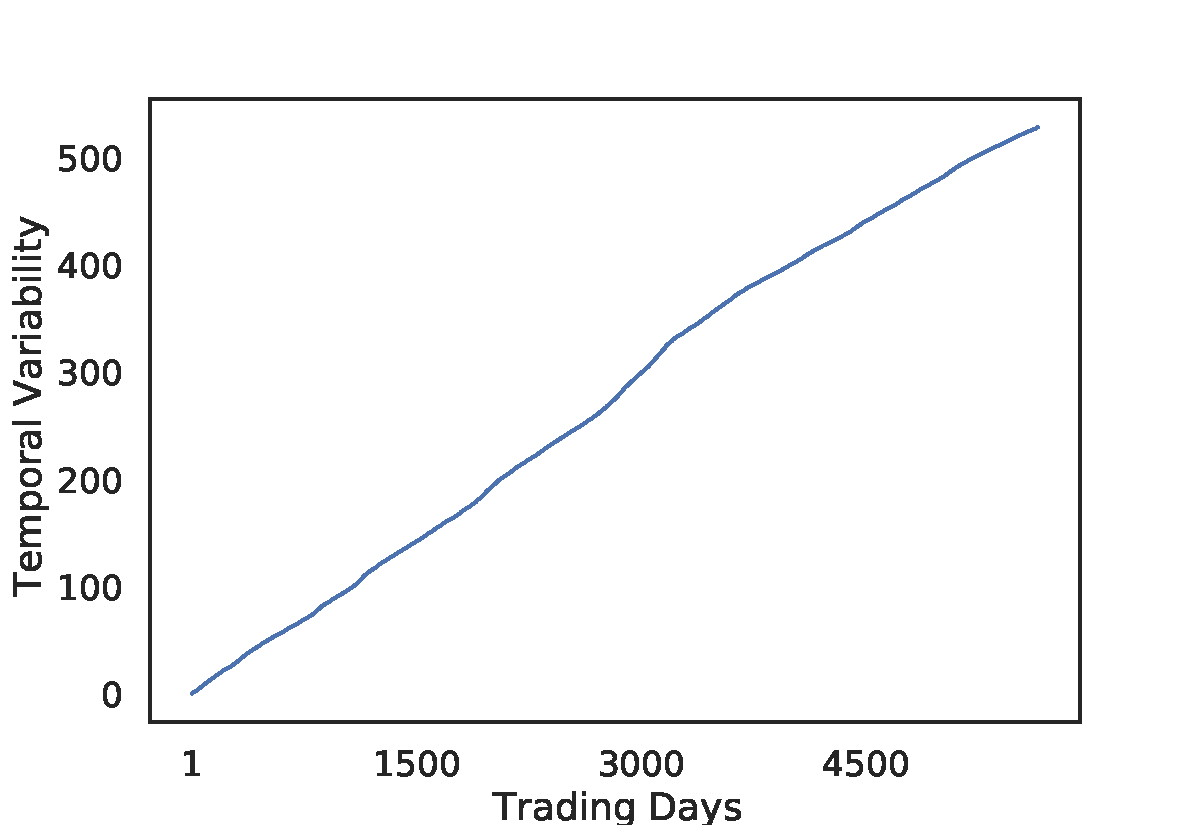
\includegraphics[width=4.5cm, keepaspectratio]{variation-functional_nyse-o} }}%
%    \,
%    \subfloat[NYSE (N)]{{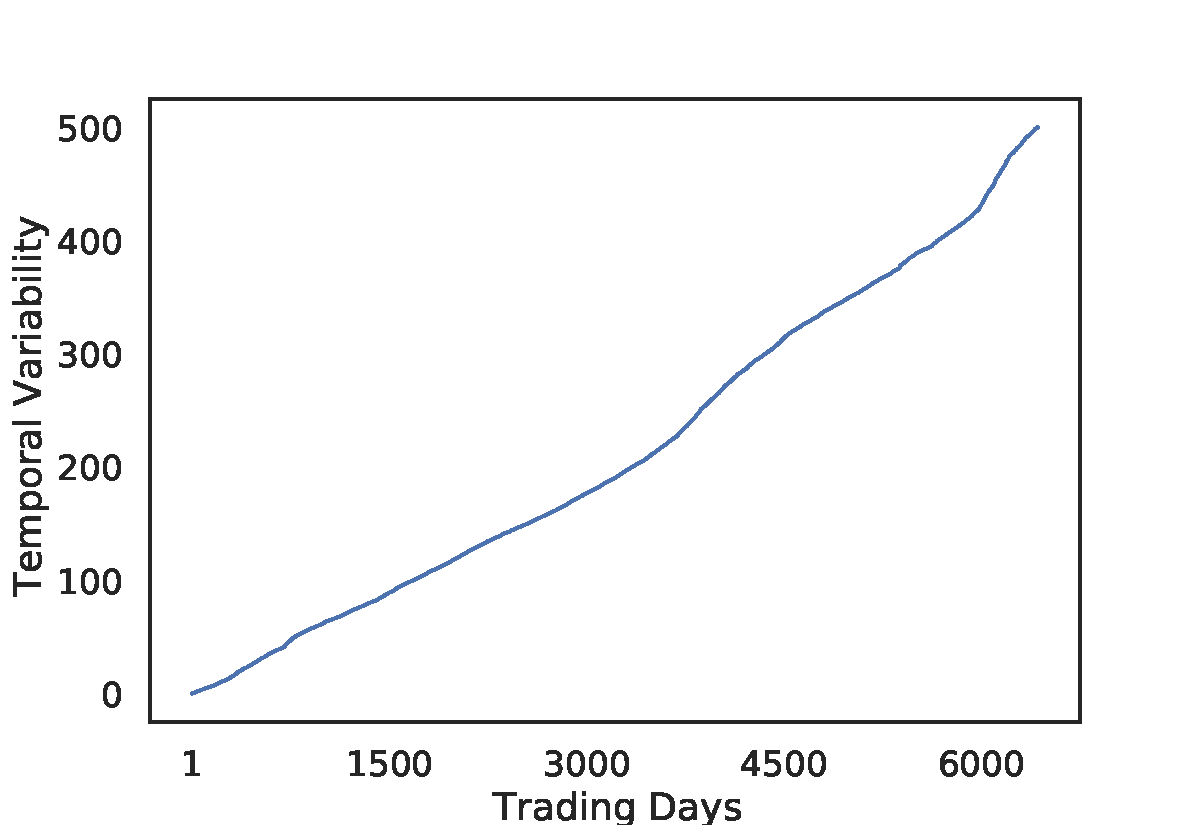
\includegraphics[width=4.5cm, keepaspectratio]{variation-functional_nyse-n} }}%
%    \,
%    \subfloat[TSE]{{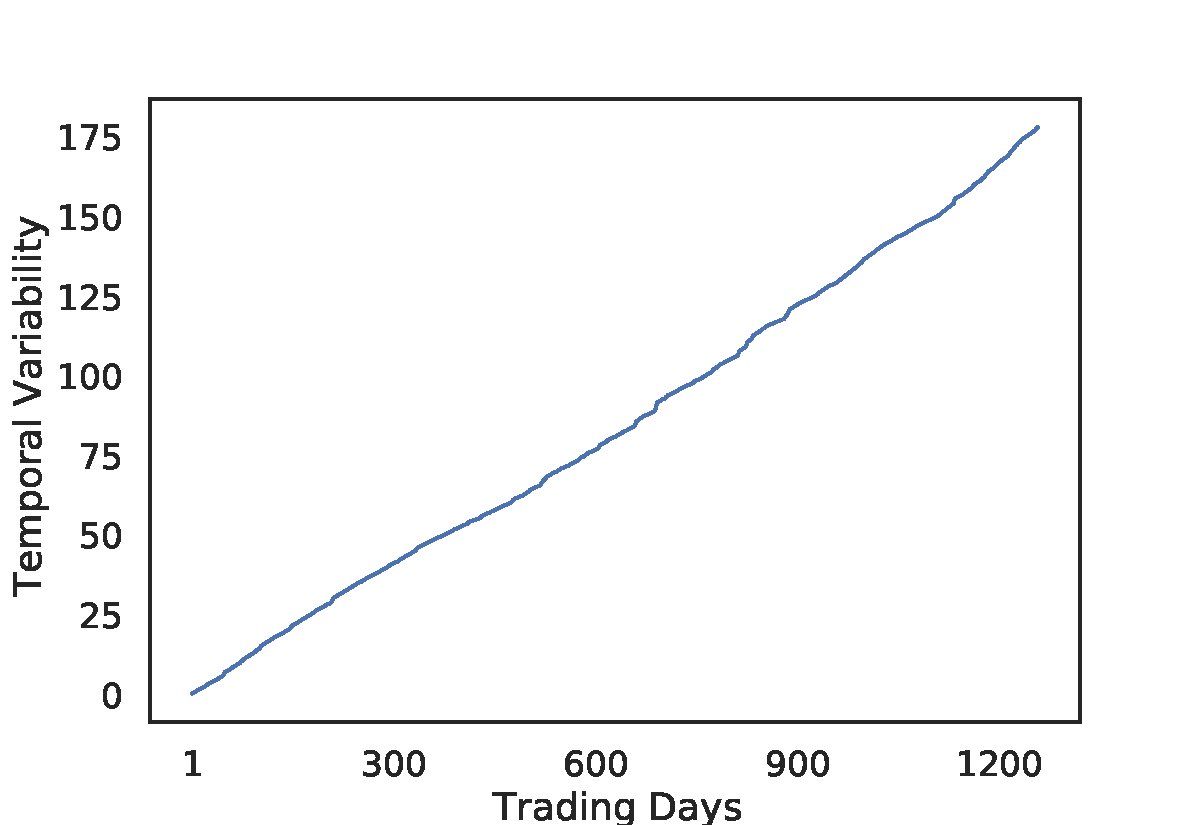
\includegraphics[width=4.5cm, keepaspectratio]{variation-functional_tse} }}%
%    
%    \subfloat[SP500]{{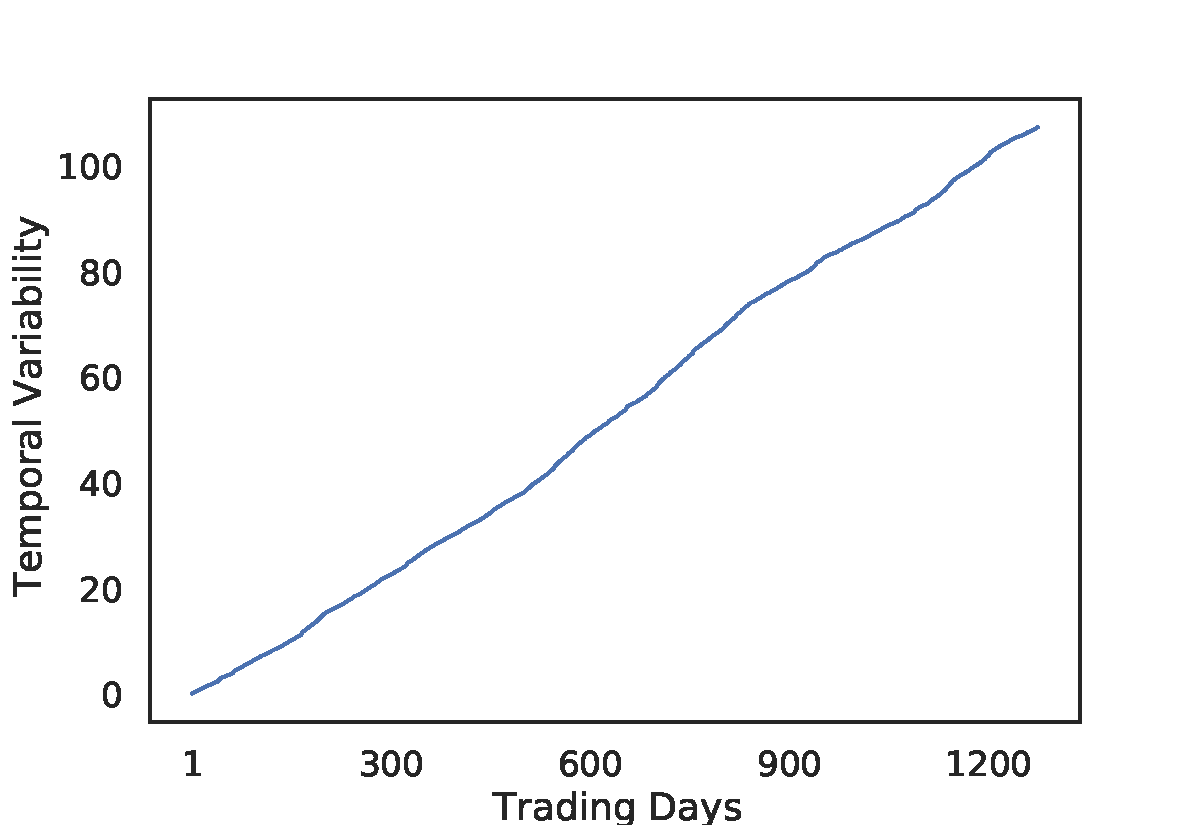
\includegraphics[width=4.5cm, keepaspectratio]{variation-functional_sp500} }}%
%    \,
%    \subfloat[MSCI]{{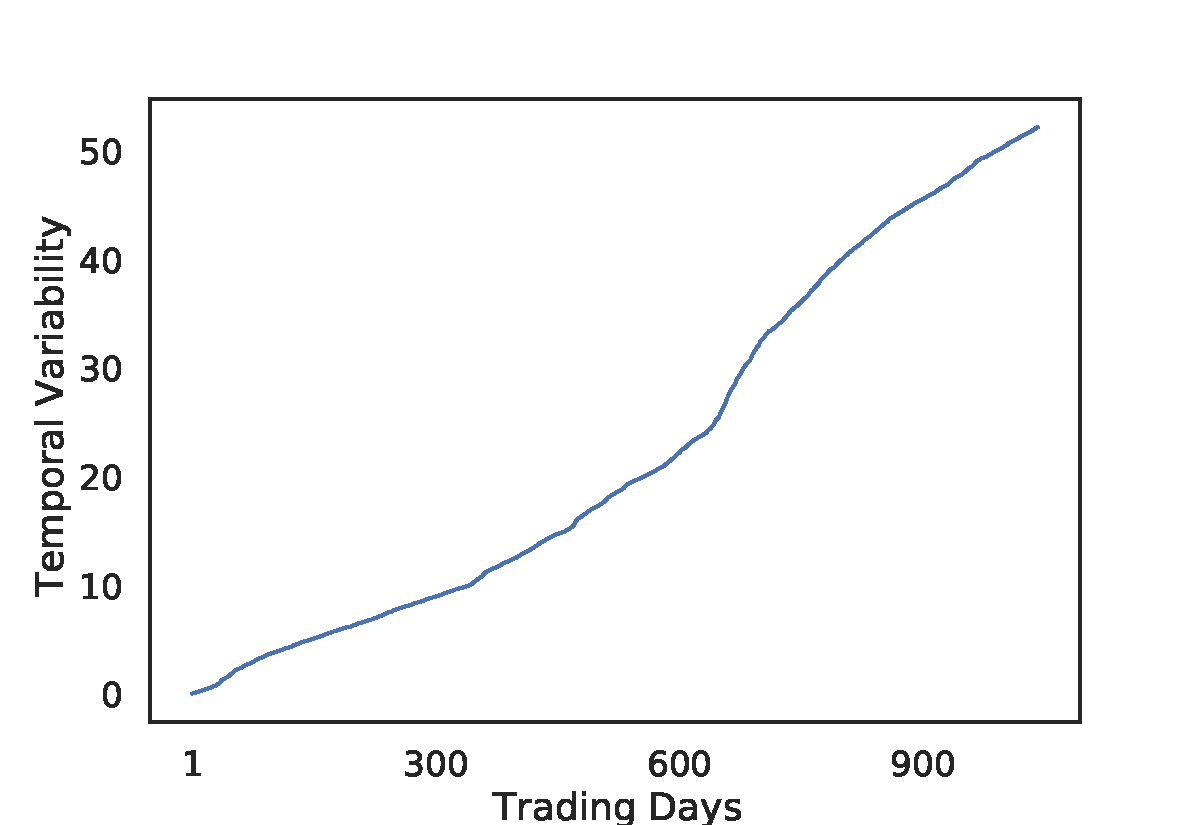
\includegraphics[width=4.5cm, keepaspectratio]{variation-functional_msci} }}%
%    \,
%    \subfloat[DJIA]{{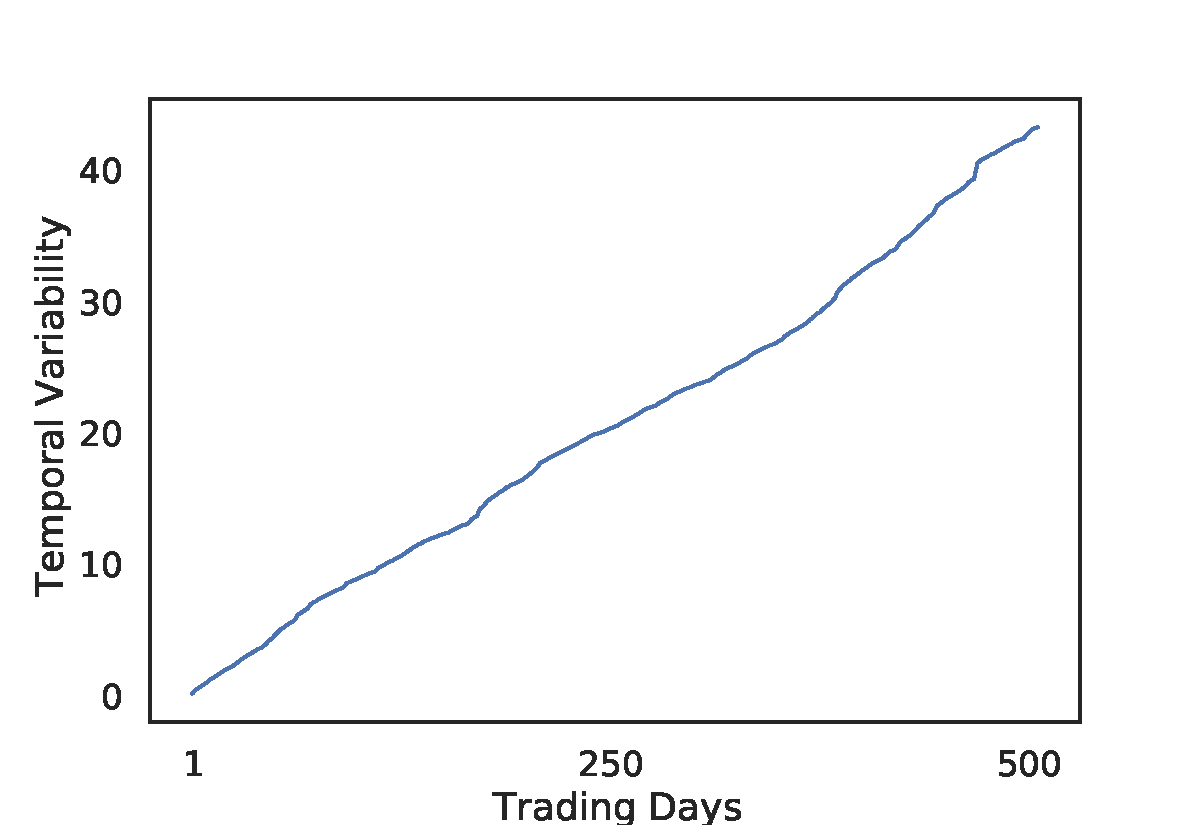
\includegraphics[width=4.5cm, keepaspectratio]{variation-functional_djia} }}%
%\end{figure}
\begin{mccorrection}
\begin{figure}[H]
\caption{Temporal variability $\mathrm{Var}(f_{1:T}) = \sum_{t=2}^T \Vert f_t - f_{t-1} \Vert_\infty$ for the six equity data sets from Table~\ref{tab:stock-datasets}. The solid red line represents the identity line (i.e. $y=x$).}
\label{fig:temporal-variation}
    \subfloat[NYSE (O)]{{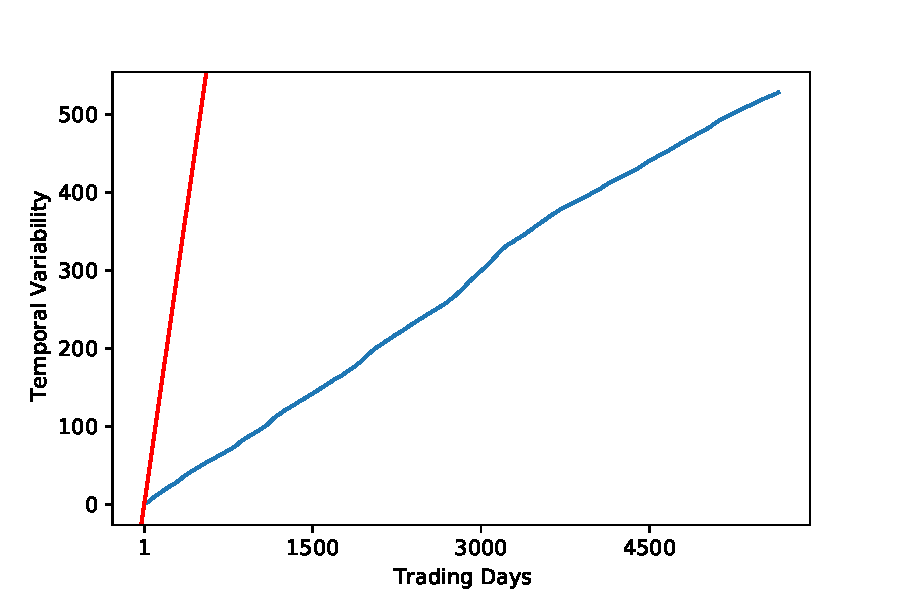
\includegraphics[width=4.5cm, keepaspectratio]{variation-functional_nyse-o_NEW} }}%
    \,
    \subfloat[NYSE (N)]{{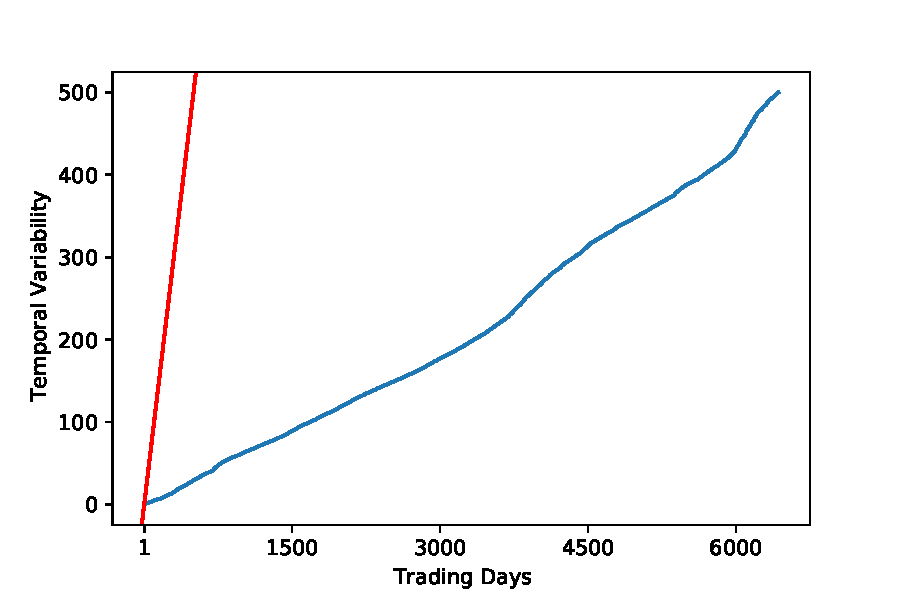
\includegraphics[width=4.5cm, keepaspectratio]{variation-functional_nyse-n_NEW} }}%
    \,
    \subfloat[TSE]{{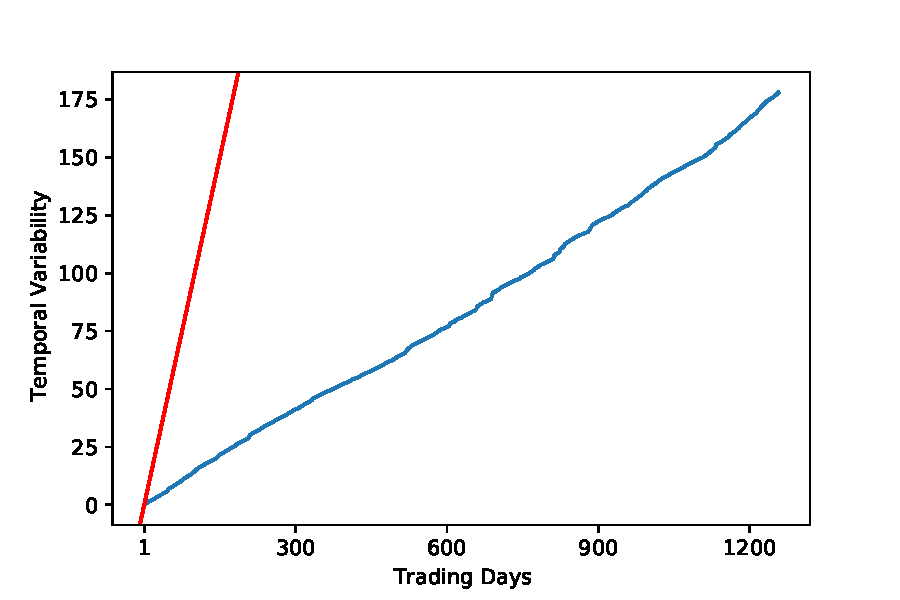
\includegraphics[width=4.5cm, keepaspectratio]{variation-functional_tse_NEW} }}%
    
    \subfloat[SP500]{{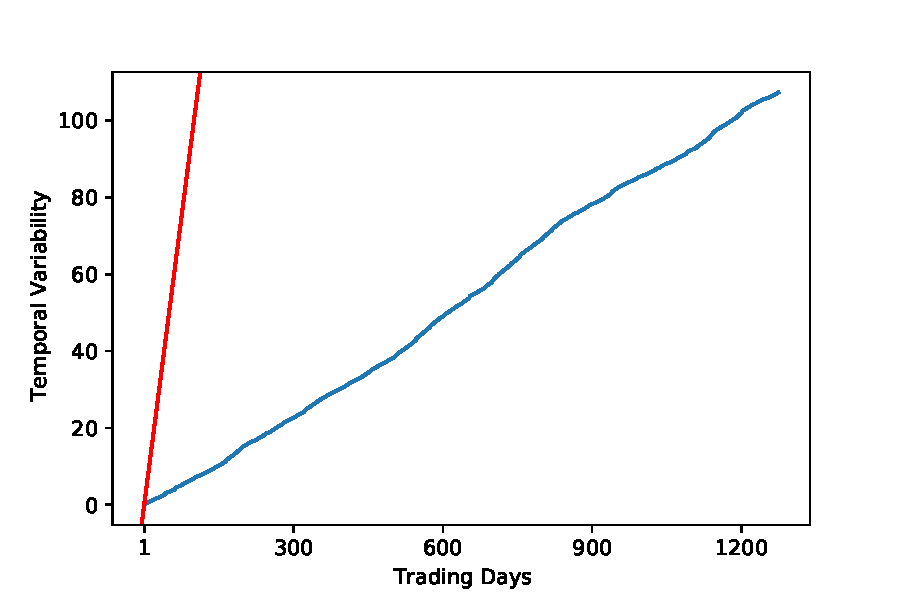
\includegraphics[width=4.5cm, keepaspectratio]{variation-functional_sp500_NEW} }}%
    \,
    \subfloat[MSCI]{{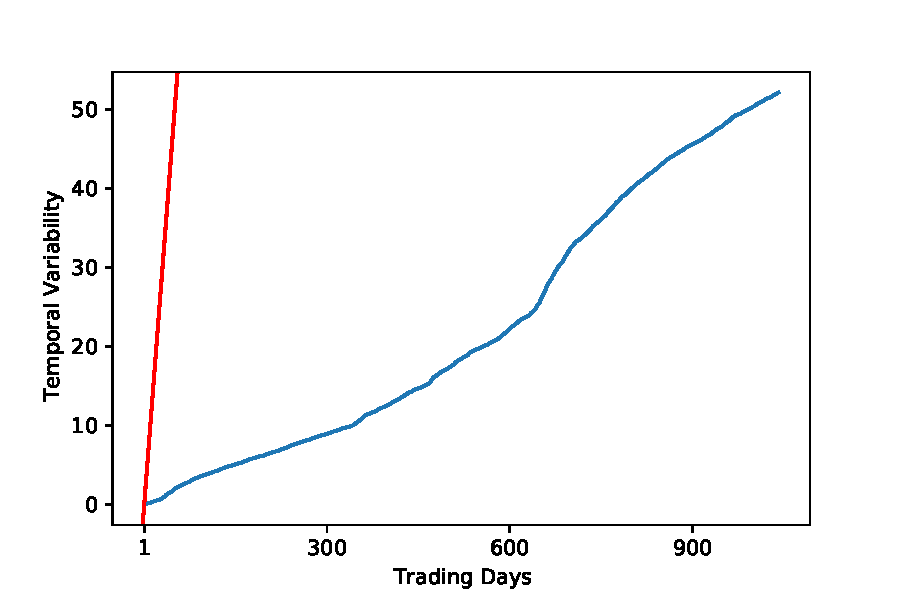
\includegraphics[width=4.5cm, keepaspectratio]{variation-functional_msci_NEW} }}%
    \,
    \subfloat[DJIA]{{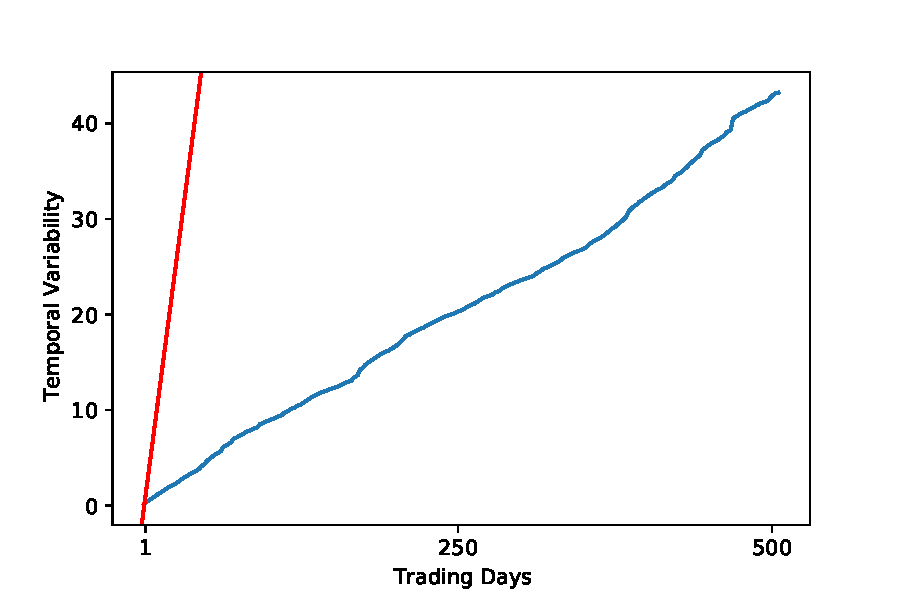
\includegraphics[width=4.5cm, keepaspectratio]{variation-functional_djia_NEW} }}%
\end{figure}
\end{mccorrection}
Figure~\ref{fig:variation-functional-boxplot} allows us to get a sense of the tracking-error magnitudes for the six equity data sets. Given the tight interquartile ranges and relatively low medians, we should not expect these to be very significant.
\begin{figure}[H]
\caption{Box plot of temporal-variability components $\Vert f_t - f_{t-1} \Vert_\infty$ across the six equity data sets presented in Table~\ref{tab:stock-datasets}.}
\label{fig:variation-functional-boxplot}
\begin{center}
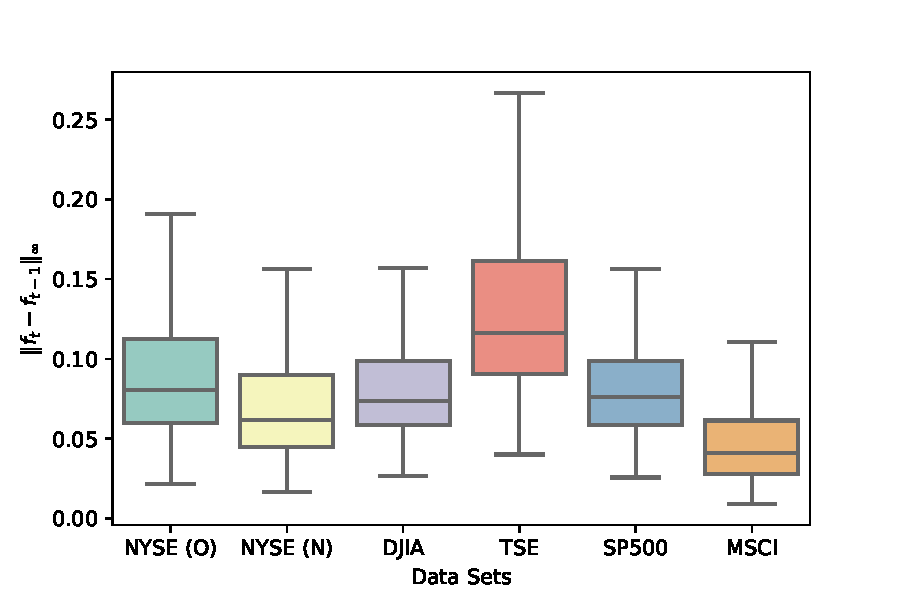
\includegraphics[width=\textwidth,height=\textheight,keepaspectratio]{variation-functional-boxplot}
\end{center}
\end{figure}

\subsection{Formulations}

\subsubsection{Single-period mean reversion}

Our single-period mean reversion algorithm, termed SingleOLMAX, is based on the single-period mean reversion ideas described in \citep[Section~4.1]{pamr}. The goal is to solve the problem in Eq. \eqref{eq:olps-problem}, with $f_t(\mathbf{b}) = \mathbf{b}^\text{T}\mathbf{x}_t$ instead of Eq. \eqref{eq:olps-loss-function}. The reason for this is because we seek to capitalise on the appreciation of poor-performing stocks, expecting their bad performance to be transient and to ultimately `revert to the mean', which calls for a \emph{follow-the-loser} investing approach.

We saw in the previous subsection that the temporal variability of the loss-function sequence is sublinear in $T$, for all the stock data sets. As shown in Proposition~\ref{prop:action-choices-dynamic-regret}, the following portfolio strategy will therefore achieve a sublinear tracking error:
\begin{equation}
\label{eq:single-olmax-criterion}
	\mathbf{b}_{t+1} \in \argmin_{\mathbf{b}\in\Delta_m}\; \mathbf{b}^\text{T}\mathbf{x}_t, \qquad t \in [T-1],
\end{equation}
with the convention that $\mathbf{b}_1 = \mathbf{1} / m$. To solve this linear program, it is convenient to first sort the components of $\mathbf{x}_t$ in ascending order, so that
\begin{equation}
	x_{t,1} \leq x_{t,2} \leq \ldots \leq x_{t,i} \leq \ldots \leq x_{t,m}.
\end{equation}
We then check the sign of $x_{t,1}$. If the latter is non-negative, then the minimal value of $\mathbf{b}^\text{T}\mathbf{x}_t$ is achieved by setting $b_{t+1,i} = 0$ for all $i\in[m]$, which, after performing the projection onto $\Delta_m$, results in the equally-weighted portfolio $\mathbf{1} / m$. Conversely, if $x_{t,1} < 0$, then the optimal weights are such that $b_{t+1,1} = 1$ and $b_{t+1,k} = 0$ for all $k > 1$. Wrapping up the two cases, we obtain the following strategy:
\begin{equation}
	b_{t+1,i} =
	\begin{cases}
		0 & \text{if } x_{t,1} \geq 0 \\
		\delta_{i1} & \text{otherwise}
	\end{cases},
	\qquad \forall\,t \in [T-1],\, \forall\,i \in [m],
\end{equation}
where $\delta_{ij}$ denotes the Kronecker delta. This choice is quite obvious: we allocate our entire budget to the investment with the lowest price relative.

The procedure is outlined in Algorithm~\ref{alg:single-period-olmax}. Note that it is completely hyperparameter-free and thereby not prone to the data-snooping bias, unlike its cousin PAMR.
\begin{algorithm}
  \caption{SingleOLMAX: Single-Period Online Maximum Reversion}
\label{alg:single-period-olmax}
  \begin{algorithmic}[1]
%    \STATE {\bfseries Input:} market sequence $\mathbf{x}_{1:T}$
    \STATE {\bfseries Initialisation:} initial portfolio $\mathbf{b}_1 = \frac{\mathbf{1}}{m}$, initial wealth $S_0 = 1$
    \FOR{$t=1, 2, \ldots, T$}
      \STATE observe stock price relatives $\mathbf{x}_t$
      \STATE update wealth:
        $
          S_t = S_{t-1} \times (\mathbf{b}_t^\text{T}\mathbf{x}_t)
        $
      \IF {$t < T$} 
        \STATE sort $\mathbf{x}_t$ in ascending order 
      \STATE update the portfolio:
	\begin{equation*}
		b_{t+1,i} =
		\begin{cases}
			0 & \text{if } x_{t,1} \geq 0 \\
			\delta_{i1} & \text{otherwise}
		\end{cases},
		\qquad i \in [m]
	\end{equation*}
	\ENDIF
    \ENDFOR
%    \STATE {\bfseries Output:} terminal wealth $S_T$
  \end{algorithmic}
\end{algorithm}

\subsubsection{Multiperiod mean reversion}

One common criticism of the single-period mean reversion assumption is that it fails to account for price reversals that occur over longer periods (see, e.g., \citep{olmar}). To overcome this limitation, we follow \citet{olmar}, and modify the SingleOLMAX criterion in Eq. \eqref{eq:single-olmax-criterion} as follows:  
\begin{equation}
\label{eq:multi-olmax-criterion}
	\mathbf{b}_{t+1} \in \argmax_{\mathbf{b}\in\Delta_m}\; \mathbf{b} \cdot \widetilde{\mathbf{x}}_{t+1}, \qquad t \in [T-1],
\end{equation}
where $\widetilde{\mathbf{x}}_{t+1}$ is a forecast of the $(t+1)$-th price-relative vector based upon the sequence $\mathbf{x}_{1:t}$ of observed price relatives. From a dynamic OCO standpoint, we can heuristically justify Eq. \eqref{eq:multi-olmax-criterion} via
\begin{equation}
	\argmax_{\mathbf{b}\in\Delta_m}\; \mathbf{b} \cdot \widetilde{\mathbf{x}}_{t+1}
	\approx \mathbf{b}_{t+1}^*,
\end{equation}
where $\mathbf{b}_{t+1}^*$ is the clairvoyant's optimal portfolio for period $(t+1)$, i.e.\ $\mathbf{b}_{t+1}^* = \argmax_{\mathbf{b}\in\Delta_m}\, \mathbf{b} \cdot \mathbf{x}_{t+1}$. By analogy with Eq. \eqref{eq:single-olmax-criterion}, after sorting $\widetilde{\mathbf{x}}_{t+1}$ in ascending order, we can write the unique solution to the optimisation problem in Eq. \eqref{eq:multi-olmax-criterion} as
\begin{equation}
	b_{t+1,i} =
	\begin{cases}
		0 & \text{if } \widetilde{x}_{t+1,m} \leq 0 \\
		\delta_{im} & \text{otherwise}
	\end{cases},
	\qquad \forall\,t \in [T-1],\, \forall\,i \in [m].
\end{equation}

We now discuss how to form the predictions $\widetilde{\mathbf{x}}_{t+1}$. The basic idea is to exploit the reversion of the current prices $\mathbf{p}_t$ to $\widetilde{\mathbf{p}}_{t+1} = \mathrm{MA}_t$, where $\mathrm{MA}_t$ denotes the moving average of price vectors at the end of period $t$. Following \citet{olmar}, we shall consider two types of moving average, namely a simple moving average (SMA)
\begin{equation}
\label{eq:sma}
	\mathrm{SMA}_t
	= \frac{1}{w}\sum_{\tau=t-w+1}^t \mathbf{p}_\tau,
\end{equation}
where $w$ denotes the size of the lookback window, and an exponential moving average (EMA)
\begin{equation}
\label{eq:ema}
	\mathrm{EMA}_t
	= \alpha\mathbf{p}_t + (1-\alpha)\mathrm{EMA}_{t-1},
\end{equation}
where $\alpha \in (0, 1)$ is the smoothing factor. The corresponding price-relative forecasts are respectively:
\begin{align}
	& \widetilde{\mathbf{x}}_{t+1}^\text{SMA}
	\equiv \frac{\mathrm{SMA}_t}{\mathbf{p}_t}
	= \frac{1}{w}\left(\frac{\mathbf{p}_t}{\mathbf{p}_t} + \frac{\mathbf{p}_{t-1}}{\mathbf{p}_t} + \ldots + \frac{\mathbf{p}_{t-w+1}}{\mathbf{p}_t}\right)
	= \frac{1}{w}\left(\mathbf{1} + \frac{1}{\mathbf{x}_t} + \ldots + \frac{1}{\bigotimes_{h=0}^{w-2}\mathbf{x}_{t-h}}\right),
	\\
	& \widetilde{\mathbf{x}}_{t+1}^\text{EMA}
	\equiv \frac{\mathrm{EMA}_t}{\mathbf{p}_t}
	= \frac{\alpha\mathbf{p}_t + (1-\alpha)\mathrm{EMA}_{t-1}}{\mathbf{p}_t}
%	= \alpha + (1-\alpha)\frac{\mathrm{EMA}_{t-1}}{\mathbf{p}_{t-1}}\frac{\mathbf{p}_{t-1}}{\mathbf{p}_t}
	= \alpha + (1-\alpha)\frac{\widetilde{\mathbf{x}}_{t}^\text{EMA}}{\mathbf{x}_t}.
\end{align}

We present the resulting two variants of our proposed multiperiod online maximum reversion (MultiOLMAX) method in Algorithm~\ref{alg:multiperiod-olmax}. Compared to their OLMAR counterparts in \citep{olmar}, they rely on a single hyperparameter instead of two, namely the window size $w$ for the SMA variant and the smoothing factor $\alpha$ for the EMA variant\footnote{OLMAR additionally depends on a reversion threshold $\epsilon$.}.
\begin{algorithm}
  \caption{MultiOLMAX: Multiperiod Online Maximum Reversion}
\label{alg:multiperiod-olmax}
  \begin{algorithmic}[1]
    \STATE {\bfseries Input:} Window size $w \geq 2$ (SMA variant), smoothing factor $0 < \alpha < 1$ (EMA variant)
    \STATE {\bfseries Initialisation:} initial portfolio $\mathbf{b}_1 = \frac{\mathbf{1}}{m}$, initial wealth $S_0 = 1$
    \FOR{$t=1, 2, \ldots, T$}
      \STATE observe stock price relatives $\mathbf{x}_t$
      \STATE update wealth:
        $
          S_t = S_{t-1} \times (\mathbf{b}_t^\text{T}\mathbf{x}_t)
        $
      \IF {$t < T$}
      	\STATE predict next price-relative vector:
	\begin{equation*}
		\widetilde{\mathbf{x}}_{t+1} =
		\begin{cases}
			\frac{1}{w}\left(\mathbf{1} + \frac{1}{\mathbf{x}_t} + \ldots + \frac{1}{\bigotimes_{h=0}^{w-2}\mathbf{x}_{t-h}}\right) & \text{(SMA variant)} \\
			\alpha + (1-\alpha)\frac{\widetilde{\mathbf{x}}_{t}}{\mathbf{x}_t} & \text{(EMA variant)}
		\end{cases}
	\end{equation*}
        \STATE sort $\widetilde{\mathbf{x}}_{t+1}$ in ascending order 
      \STATE update the portfolio:
	\begin{equation*}
		b_{t+1,i} =
	\begin{cases}
		0 & \text{if } \widetilde{x}_{t+1,m} \leq 0 \\
		\delta_{im} & \text{otherwise}
	\end{cases},
	\qquad i \in [m].
	\end{equation*}
	\ENDIF
    \ENDFOR
%    \STATE {\bfseries Output:} terminal wealth $S_T$
  \end{algorithmic}
\end{algorithm}


\section{Experiments}
\label{sec:experiments}

In this section, we will present an extensive set of empirical studies, including our experimental test bed, protocols, comparison schemes, results and a detailed empirical analysis.

\subsection{Experimental test bed on real data}

To be able to compare the empirical performance of our OLMAX framework against that of other OLPS strategies, we focus on historical daily stock prices. Earlier studies have restricted their empirical analyses to equity data as they can be readily obtained from public domains such as Yahoo! Finance and Google Finance\footnote{Yahoo! Finance: \url{https://finance.yahoo.com/}; Google Finance: \url{https://www.google.com/finance}.}, which ensures experimental reproducibility. Summarised in Table~\ref{tab:stock-datasets}, we employ six real and diverse data sets from several financial markets\footnote{The data sets from \citep{borodin04} --- NYSE (O), TSE, SP500 and DJIA --- can be found at \url{http://www.cs.technion.ac.il/~rani/portfolios/}. As for the remaining data sets and their respective composition, they can be downloaded from \url{http://www.cais.ntu.edu.sg/~chhoi/olps}.}.

The first data set, NYSE (O), is a standard data set pioneered by \citet{cover} and used in subsequent works \citep{eg, borodin04, ons, bnn}. This data set contains 5,651 daily price relatives of 36 stocks\footnote{According to \citet{eg}, the data set was originally collected by Hal Stern. The stocks are mainly those of large-cap companies listed on NYSE. However, we ignore the criteria that were used in selecting them.} from the New York Stock Exchange (NYSE) over a 22-year period from July 3, 1962 until December 31, 1984.

The second data set, NYSE (N), is an extended version of NYSE (O) collected by \citet{cwmr}. It covers the period from January 1, 1985 to June 30, 2010, i.e.\ a total of 6,431 trading days\footnote{The data before 2007 were collected by G\'{a}bor Gelencs\'{e}r \url{http://www.cs.bme.hu/~oti/portfolio/}, whereas \citet{cwmr} collected the remaining data from Yahoo! Finance.}. Note that it is limited to 23 rather than 36 stocks owing to mergers and bankruptcies.

The third and fourth data sets, TSE and SP500, were collected by \citet{borodin04}. The former consists of 88 stocks listed on the Toronto Stock Exchange (TSE) and contains price relatives over a period of 1,259 trading days, ranging from January 4, 1994 through December 31, 1998. As for SP500, it consists of the 25 stocks in the S\&P500 index with the largest market capitalisations. It ranges from January 2, 1998 to January 31, 2003 (1,276 trading days).

The fifth dataset is MSCI, which is a collection of global equity indices that constitute the MSCI World Index\footnote{The constituents of this index are available at MSCI Barra (https://www.msci.com/).}. It is made of 24 indices that represent the equity markets of 24 countries around the world and spans of a total of 1,043 trading days, ranging from April 1, 2006 to March 31, 2010. The final dataset is the DJIA dataset \citep{borodin04}, consisting of the 30 components of the Dow Jones Industrial Average index. DJIA contains 507 trading days, ranging from January 14, 2001 to January 14, 2003.

The above test bed enables us to examine the behaviour of the proposed strategies under different market circumstances. For example, it covers several well-known crises in equity markets, such as the dot-com bubble from 1995 to 2000 and the subprime mortgage crisis from 2007 to 2009. The main purpose of the five stock data sets is to test the capabilities of the proposed algorithms on regional stock markets, while the MSCI index data set aims to assess their empirical performance on global indices.

\subsection{Experimental setup and metrics}

Our experimental setup is as follows. For MultiOLMAX (Algorithm~\ref{alg:multiperiod-olmax}), we denote by MultiOLMAX-S and MultiOLMAX-E the variants with SMA and EMA forecasts, respectively. To make our results comparable to those of \citet{olmar}, we adopt their hyperparameter configuration, namely $w = 5$ and $\alpha = 0.3$, across all six equity data sets. We shall assess the sensitivity of OLMAX to hyperparameter selection in Section~\ref{sec:olmax-hyperparameter-sensitivity}.

Following the standard practice in the OLPS literature, we primarily compare different strategies in terms of terminal wealth and annualised Sharpe ratio \citep{sharpe}. In general, higher values of these metrics indicate better algorithms. To analyse a strategy's downside risk, we use the maximum drawdown (MDD) metric; the lower the MDD values, the less pronounced the strategy's downside. For convenience, we report all these metrics in Table~\ref{tab:metrics}.
\begin{table}[t]
  \caption{Summary of the performance metrics used in the evaluations.}
  \label{tab:metrics}
  \centering
  \resizebox{\textwidth}{!}{\begin{tabular}{lc}
    \toprule
    Critetion & Performance metrics \\
    \midrule
    Absolute return & Terminal wealth ($S_T$), Annual percentage yield (APY) \\
    Risk & Annualised standard deviation, Maximum drawdown (MDD) \\
    Risk-adjusted return & Annualised Sharpe ratio (SR) \\
    \bottomrule
  \end{tabular}}
\end{table}

\begin{mccorrection}
There is somewhat of a disconnect of the metrics used for benchmarking and the notion of regret, in the sense that while the performance metrics from Table~\ref{tab:metrics} are meaningful, the algorithms proposed in this thesis were devised in the spirit of regret. However, we refrained from measuring performance relative to regret as well because most of the OLPS techniques used for benchmarking purposes in this chapter do not optimise regret, but rather obey alternative optimisation criteria. Therefore, while we could have computed the regret of these OLPS methods and compare it against the regret of our proposed methods, we thought it would have been unfair towards these methods.
\end{mccorrection}

In the next subsection, we discuss one important practical issue in online portfolio selection, namely transaction costs. We defer the evaluation of the performance of OLMAX under transaction costs to Section~\ref{sec:transaction-costs}.

\subsection{Transaction costs}

While our model in Section~\ref{sec:olps-model} is concise and easy to understand, it omits the important and unavoidable issue of \emph{transaction costs}, which include commission fees and taxes imposed by brokers and governments, respectively\footnote{Besides these, other factors such as bid-ask spreads contribute to transaction costs.}.

Basically, there are two ways to handle the transaction-cost issue. The first is to omit transaction costs from the OLPS model in the first instance to then adopt the \emph{proportional transaction cost} model \citep{blum99}. The second is to directly integrate the costs into the model \citep{gyorfi08}. Since the former approach is the most common in the OLPS literature, we shall follow it here. Specifically, at the beginning of period $t$, the portfolio manager rebalances to a new portfolio $\mathbf{b}_t$ from the last close-price adjusted portfolio $\widehat{\mathbf{b}}_{t-1}$, each component of which is calculated as $\widehat{b̂}_{t-1,i} = \frac{b_{t-1,i} \times x_{t-1,i}}{\mathbf{b}_{t-1}^\text{T}\mathbf{x}_{t-1}}$. Letting $\gamma \in (0, 1)$ be the transaction-cost rate, this rebalancing step incurs a transaction cost of $\frac{\gamma}{2}\sum_{i=1}^m |b_{t,i} - \widehat{b̂}_{t-1,i}|$, with the initial portfolio being set to the zero vector. Thus, the wealth after $T$ periods can be expressed as
\begin{equation}
	S_T^\gamma
	= S_0 \prod_{t=1}^T \left[(\mathbf{b}_t^\text{T}\mathbf{x}_t) \times \left(1 - \frac{\gamma}{2}\sum_{i=1}^m |b_{t,i} - \widehat{b̂}_{t-1,i}|\right)\right].
\end{equation}

\subsection{Comparison approaches}
\label{sec:comparison-approaches}

We shall compare the proposed algorithms against a number of benchmarks and representative strategies enumerated below, all of which provide extensive empirical evaluations in their respective studies. All parameters are set to the same values used in the corresponding papers\footnote{We could tune these parameters to improve performance, but this is beyond the scope of this thesis.}. Because this chapter has an empirical focus, we omit algorithms that place an emphasis on theoretical analysis and lack thorough experimentation.
\begin{enumerate}
  \item Market: Market strategy, that is, the uniform buy-and-hold (BAH) strategy;
  \item Best stock: Stock with the best performance in hindsight throughout the $T$-period horizon;
%  \item CRP: Constant Rebalanced Portfolio strategy \citep{cover};
%  \item UCRP: Uniform Constant Rebalanced Portfolio strategy \citep{cover};
  \item BCRP: Best constant rebalanced portfolio strategy in hindsight \citep{cover};
  \item UP: Cover's universal portfolios, based on the implementation of \citet{kalai02}, in which the parameters are such that $\delta_0 = 0.004$, $\delta = 0.005$, $m = 100$ and $S = 500$;
  \item EG: Exponentiated gradient algorithm with the best learning rate $\eta = 0.05$, as suggested by \citet{eg};
  \item ONS: Online Newton step with the parameters suggested by \cite{ons}, i.e.\ $\eta = 0$, $\beta = 1$ and $\gamma = \frac{1}{8}$;
  \item Anticor: BAH$_{30}$(Anticor), i.e.\ uniform buy-and-hold investment on the algorithms Anticor$_w$ with $w = 2, 3, \ldots, 30$, which achieves the best performance among the three solutions proposed by \citet{borodin04};
  \item $\text{B}^\text{K}$: Non-parametric kernel-based moving window strategy with $W = 5$, $L = 10$ and threshold $c = 1.0$, which exhibits the best empirical performance according to \citet{bnn};
   \item $\text{B}^\text{NN}$: Non-parametric nearest-neighbour strategy with parameter values $W = 5$, $L = 10$ and $p_l = 0.02 + 0.5\frac{l-1}{L-1}$, as \citet{bnn2} suggested;
  \item CORN: Correlation-driven non-parametric learning approaches \citep{corn} with parameters $W = 5$, $P = 1$ and $\rho = 0.1$.
  \item PAMR: Passive-aggressive mean reversion \citep{pamr} with parameter $\epsilon=0.5$;
  \item CWMR: Confidence-weighted mean reversion \citep{cwmr} algorithm (exact version) with $\epsilon = 0.5$;
  \item OLMAR-S: Online moving average reversion \citep{olmar} with SMA price-relative forecasts, and parameters $\epsilon = 10$ and $w = 5$;
  \item OLMAR-E: Online moving average reversion \citep{olmar} with EMA price-relative forecasts, and parameters $\epsilon = 10$ and $\alpha = 0.3$.
%  \item RMR: Robust Median Reversion \citep{rmr} with parameters $W = 5$, $\epsilon = 10$ and $\tau = 0.001$;
%  \item OLPAPS: Online Passive-Aggressive Portfolio Selection (Algorithms~\ref{alg:olpaps-I} and~\ref{alg:olpaps-II}) with $\epsilon = 0.01$;
%  \item Kelly: \href{https://en.wikipedia.org/wiki/Kelly_criterion#Application_to_the_stock_market}{Kelly criterion};
\end{enumerate}
%The above list is also summarised in Table~\ref{olps-algos}.
%\begin{table}
%  \caption{OLPS algorithms evaluated and compared in our experiments.}
%  \label{olps-algos}
%  \centering
%  \resizebox{\textwidth}{!}{\begin{tabular}{lccc}
%    \toprule
%    Algorithm & Acronym & Type & Reference \\
%    \midrule
%    Buy and Hold & BAH & Benchmark & n/a \\
%    Constant Rebalanced Portfolio & CRP & Benchmark & \cite{cover} \\
%    Uniform CRP & UCRP & Benchmark & \cite{cover} \\
%    Best CRP & BCRP & Benchmark & \cite{cover} \\
%    Exponential Gradient & EG & Follow the Winner & \cite{eg} \\
%    Online Newton Step & ONS & Follow the Winner & \cite{ons} \\
%    Anticorrelation & Anticor & Follow the Loser & \cite{anticor} \\
%    Passive Aggressive Mean Reversion & PAMR & Follow the Loser & \cite{pamr} \\
%    Confidence Weighted Mean Reversion & CWMR & Follow the Loser & \cite{cwmr} \\
%    On-Line Moving Average Reversion & OLMAR & Follow the Loser & \cite{olmar} \\
%    Robust Median Reversion & RMR & Follow the Loser & \cite{rmr} \\
%    On-Line Passive-Aggressive Portfolio Selection & OLPAPS & Follow the Loser & this thesis \\
%    Kelly fractional betting & Kelly & Pattern Matching & \href{https://en.wikipedia.org/wiki/Kelly_criterion#Application_to_the_stock_market}{Kelly criterion} \\
%    Correlation-driven non-parametric learning & CORN & Pattern Matching & \cite{corn} \\
%    \bottomrule
%  \end{tabular}}
%\end{table}

\subsection{Experimental results -- terminal wealth}

Table~\ref{tab:terminal-wealth} reports the terminal wealth achieved by various approaches on the six equity data sets listed in Table~\ref{tab:stock-datasets}. From this perspective, the OLMAX algorithms are among the top two performers across five data sets (the exception being MSCI), and they achieve the best performance on four of them. On the well-known benchmark NYSE (O) data set, OLMAX significantly outperforms the state of the art, and likewise on the TSE and SP500 data sets. Although most existing algorithms other than Anticor and OLMAR-S perform badly on the DJIA data set, OLMAX achieves the highest final wealth, which further motivates the main idea behind the framework (see Section~\ref{sec:olmax-motivation}). Besides, the use of exponential rather than simple moving averages provides a significant performance boost on the NYSE (O) and NYSE (N) data sets.
\begin{table}[H]
  \caption{Terminal wealth achieved by various OLPS strategies on the six equity data sets from Table~\ref{tab:stock-datasets}. The top two results on each data set are highlighted in \textbf{bold}.}
  \label{tab:terminal-wealth}
  \centering
  \resizebox{\textwidth}{!}{\begin{tabular}{lcccccc}
    \toprule
    Methods & NYSE (O) & NYSE (N) & DJIA & TSE & SP500 & MSCI \\
    \midrule
	Market & 14.50 & 18.06 & 0.76 & 1.61 & 1.34 & 0.91 \\
	Best stock & 54.14 & 83.51 & 1.19 & 6.28 & 3.78 & 1.50 \\
	BCRP & 250.60 & 120.32 & 1.24 & 6.78 & 4.07 & 1.51 \\
%	UP & 26.99 & 31.07 & 0.81 & 1.59 & 1.64 & 0.92 \\
	\\
	UP & 26.68 & 31.49 & 0.81 & 1.60 & 1.62 & 0.92 \\
	EG & 27.09 & 31.00 & 0.81 & 1.59 & 1.63 & 0.93 \\
%	ONS & 109.28 & 21.43 & 1.53 & 1.62 & 3.34 & 0.86 \\
	ONS & 109.19 & 21.59 & 1.53 & 1.62 & 3.34 & 0.86 \\
	\\
	$\text{B}^\text{K}$ & 1.08E+09 & 4.64E+03 & 0.68 & 1.62 & 2.24 & 2.64 \\
	$\text{B}^\text{NN}$ & 3.35E+11 & 6.80E+04 & 0.88 & 2.27 & 3.07 & 13.47 \\
	CORN & 1.48E+13 & 5.37E+05 & 0.84 & 3.56 & 6.35 & \textbf{26.10} \\
	\\
	Anticor & 2.41E+08 & 6.21E+06 & \textbf{2.29} & 39.36 & 5.89 & 3.22 \\
	PAMR & 5.14E+15 & 1.25E+06 & 0.68 & 264.86 & 5.09 & 15.23 \\
%	CWMR & 5.55E+15 & 1.31E+06 & 0.68 & 193.86 & 4.98 & 14.93 \\
	CWMR & 6.49E+15 & 1.41E+06 & 0.68 & 332.62 & 5.90 & 17.28 \\
%	OLMAR & 7.88E+16 & 4.23E+08 & 2.26 & 58.59 & 16.37 & 14.72 \\
	\\
	OLMAR-S & 3.68E+16 & 2.54E+08 & 2.12 & 424.80 & 5.83 & 16.39 \\
	OLMAR-E & \textbf{1.09E+18} & \textbf{5.10E+08} & 1.20 & \textbf{678.44} & 8.63 & \textbf{21.21} \\
	\\
	SingleOLMAX & 4.09E+15 & 5.09E+05 & 0.59 & \textbf{1.56E+03} & 8.32 & 7.30 \\
	MultiOLMAX-S & 4.47E+16 & 3.86E+08 & \textbf{2.51} & 75.88 & \textbf{15.30} & 11.19 \\
	MultiOLMAX-E & \textbf{2.54E+18} & \textbf{4.80E+08} & 1.22 & 313.09 & \textbf{14.31} & 13.44 \\
%	\\
%	AdaPAMR & 1.08E+07 & 3.03E+05 & 0.69 & 216.69 & 6.90 & 15.06 \\
%	AdaOLMAR & 6.82E+04 & 774.05 & 2.16 & 25.33 & 5.86 & 4.10 \\
%	\\
%	MAPGRAD & 1.11E+08 & 1.79E+05 & 0.67 & 222.35 & 6.85 & 13.82 \\
    \bottomrule
  \end{tabular}}
\end{table}
In order to confirm that the above OLMAX results are not a statistical fluke, we compute the alphas and betas from the regression
\begin{equation}
	r_t^\text{OLMAX} - r_f
	= \alpha + \beta(r_t^\text{MKT} - r_f) + \varepsilon_t,
\end{equation}
where $r_t^\text{OLMAX}$ denotes the return of an OLMAX portfolio at time $t$, $r_f$ is the risk-free rate, and $r_t^\text{MKT}$ represents a passive exposure to the stock market, proxied by the return on the BAH strategy. Table~\ref{tab:stat-tests} displays the $t$-statistics and $p$-values of the estimated alphas for the MultiOLMAX-S variant. From this table, we see that the probability that the outstanding MultiOLMAX-S performance is due to luck is at most 1.31\%. Though we omitted them here, the findings are similar for other OLMAX variants. Thus, we can claim with almost absolute certainty that OLMAX outperforms the state of the art on the equity data sets.
\begin{table}[H]
  \caption{Statistical tests of the performance achieved by the MultiOLMAX-S algorithm on the stock data sets. The acronym MER stands for `mean excess return'.}
  \label{tab:stat-tests}
  \centering
  \resizebox{\textwidth}{!}{\begin{tabular}{lcccccc}
    \toprule
    Stat. Attr. & NYSE (O) & NYSE (N) & DJIA & TSE & SP500 & MSCI \\
    \midrule
	Size & 5651 & 6431 & 507 & 1259 & 1276 & 1043 \\   
	MER (MultiOLMAX-S) & 0.0073 & 0.0035 & 0.0022 & 0.0050 & 0.0026 & 0.0025 \\ 
%	MER (Market) & 0.0004 & 0.0004 & -0.0006 & 0.0003 & 0.0002 & -0.0001 \\
	MER (Market) & 0.0005 & 0.0005 & -0.0004 & 0.0004 & 0.0003 & 0.0000 \\
	Winning Ratio & 57.95\% & 55.19\% & 53.77\% & 55.15\% & 52.51\% & 55.88\% \\
	\\
	$\alpha$ & 0.0068 & 0.0031 & 0.0029 & 0.0046 & 0.0023 & 0.0026 \\   
	$\beta$ & 1.2709 & 1.1407 & 1.2540 & 1.6497 & 1.2541 & 1.1921 \\
	\\   
	$t$-stat & 15.1105 & 7.5234 & 2.4888 & 2.7452 & 2.9378 & 5.1207 \\   
	$p$-value & 0.0000 & 0.0000 & 0.0131 & 0.0061 & 0.0034 & 0.0000 \\  
    \bottomrule
  \end{tabular}}
\end{table}

\subsection{Experimental results -- risk-adjusted returns}

We now evaluate the volatility and maximum drawdown of different OLPS strategies, as well as their respective risk-adjusted returns as measured by the annualised Sharpe ratio \citep{sharpe}. Figure~\ref{fig:stock-metrics} displays these metrics for the six equity data sets. In addition to the proposed MultiOLMAX-S algorithm, we plot two benchmarks (Market and BCRP) and five state-of-the-art algorithms (Anticor, CORN, PAMR, CWMR and OLMAR\footnote{Henceforth, the acronym `OLMAR' will refer to the OLMAR-S strategy, i.e.\ the variant with SMA forecasts of price relatives.}).

In the previous paragraph, we saw that MultiOLMAX-S achieves the highest cumulative return on the majority of equity data sets. However, high return is typically associated with high risk. This is corroborated by Figures~\ref{fig:stock-metrics}(a) and (b), which show that the proposed method is one the riskiest in terms of volatility and maximum drawdown, respectively.

However, in spite of its high risk, MultiOLMAX-S yields a highly competitive Sharpe ratio, as illustrated by Figure~\ref{fig:stock-metrics}(c). This encouraging finding demonstrates that the proposed method is able to strike a good balance between risk and return, even though we do not explicitly account for risk in its formulation.

\begin{figure}[htp]
\caption{\footnotesize Risk and risk-adjusted performance of various OLPS strategies on the six stock data sets. In each diagram, the rightmost bar represents the result of our proposed strategy.}
\label{fig:stock-metrics}
\centering

\subfloat[Volatility Risk]{%
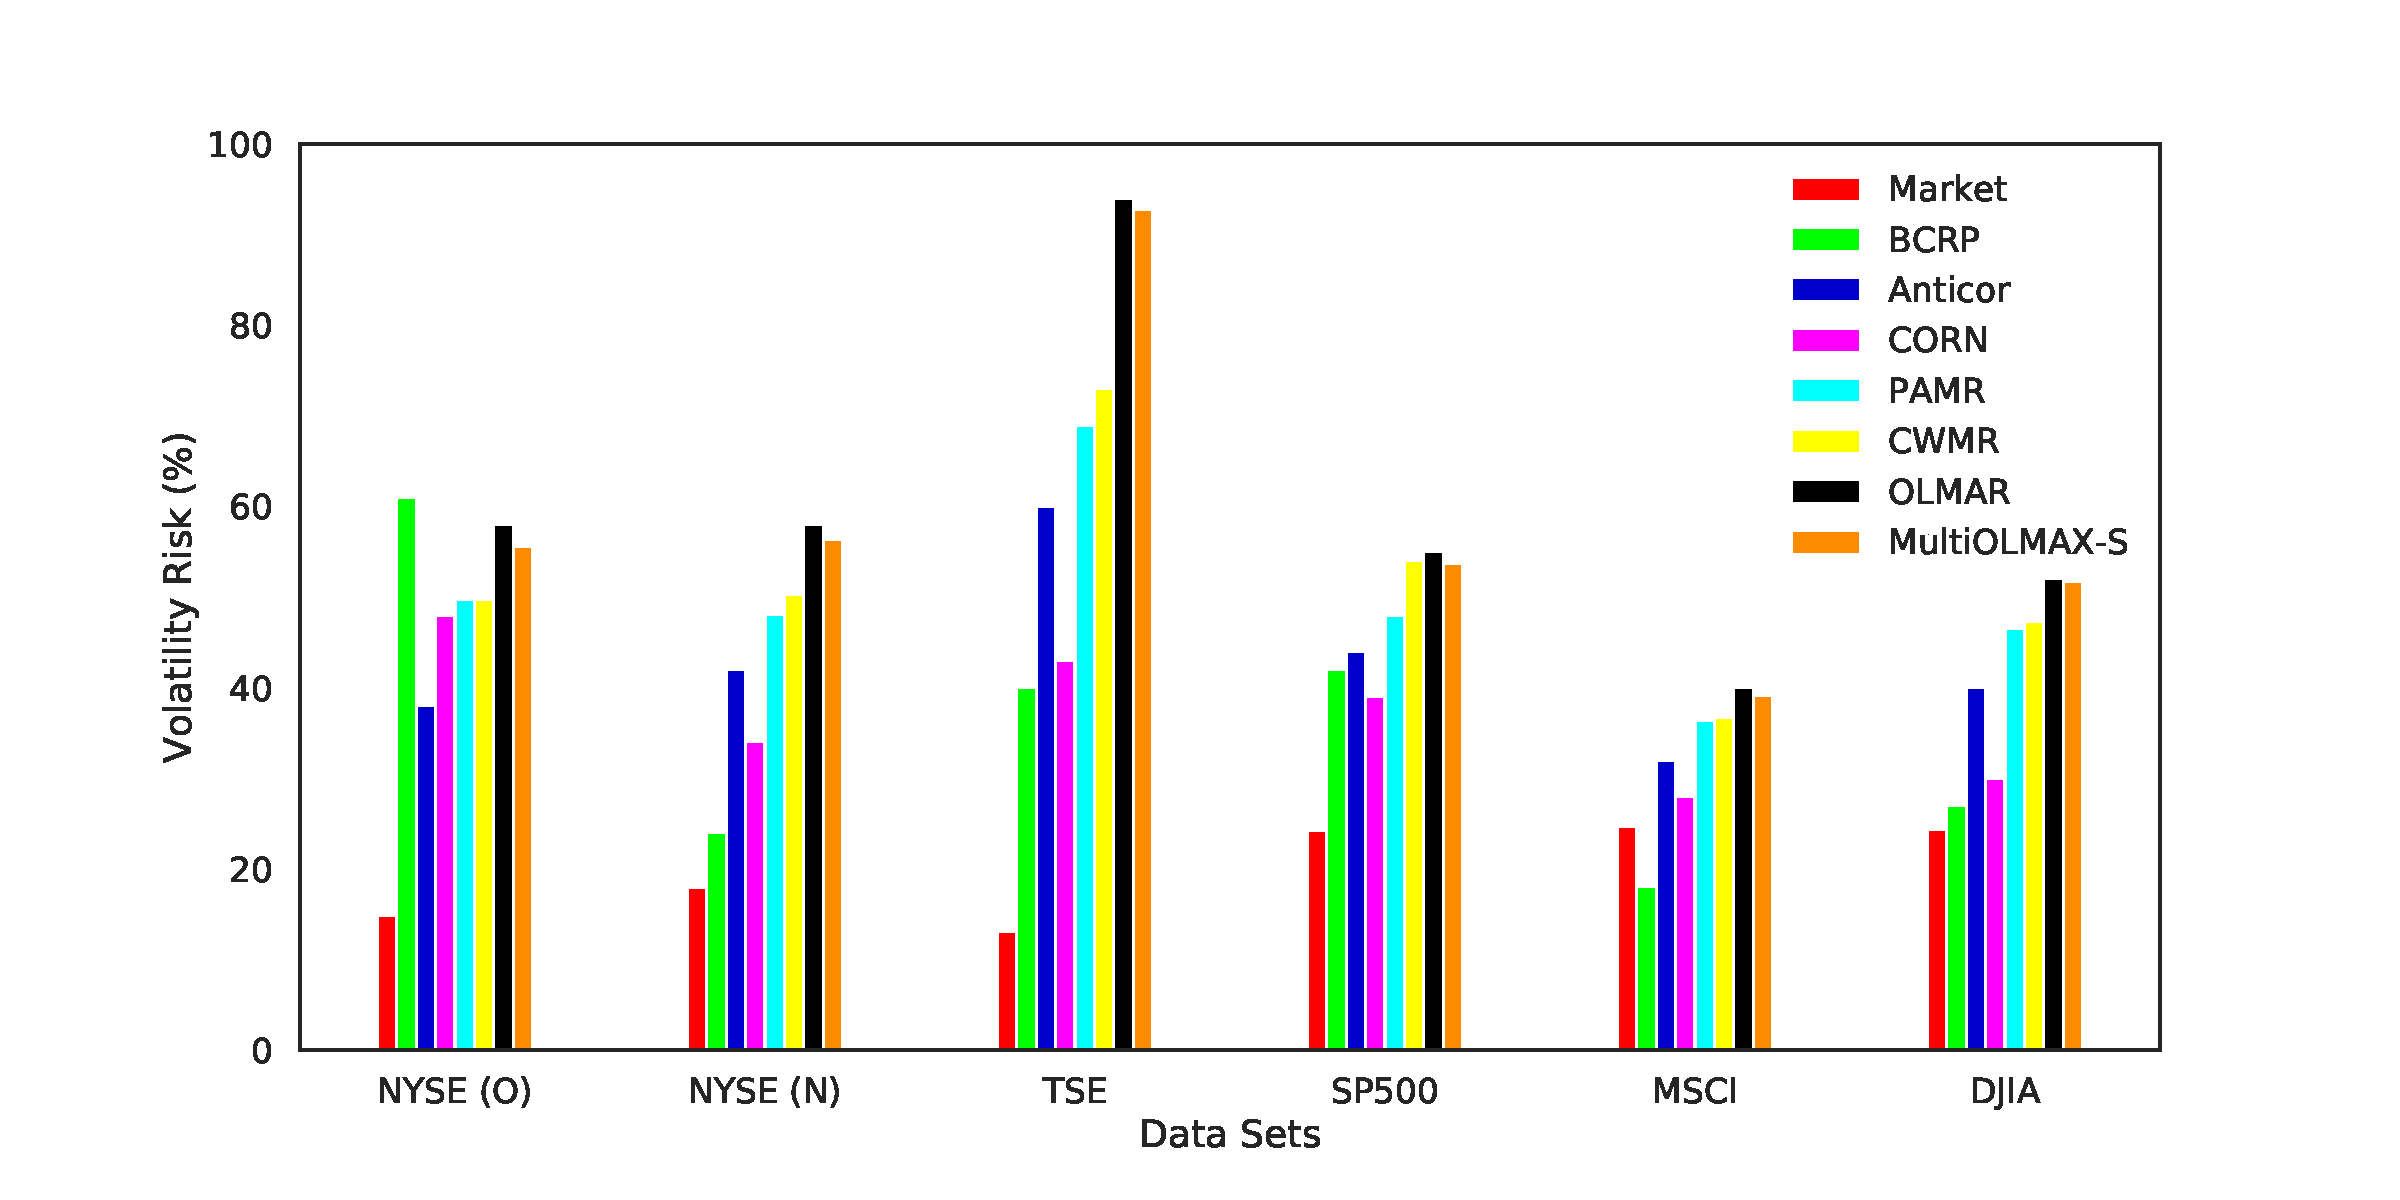
\includegraphics[width=\textwidth,height=\textheight,keepaspectratio]{vols}%
}

\subfloat[Drawdown Risk]{%
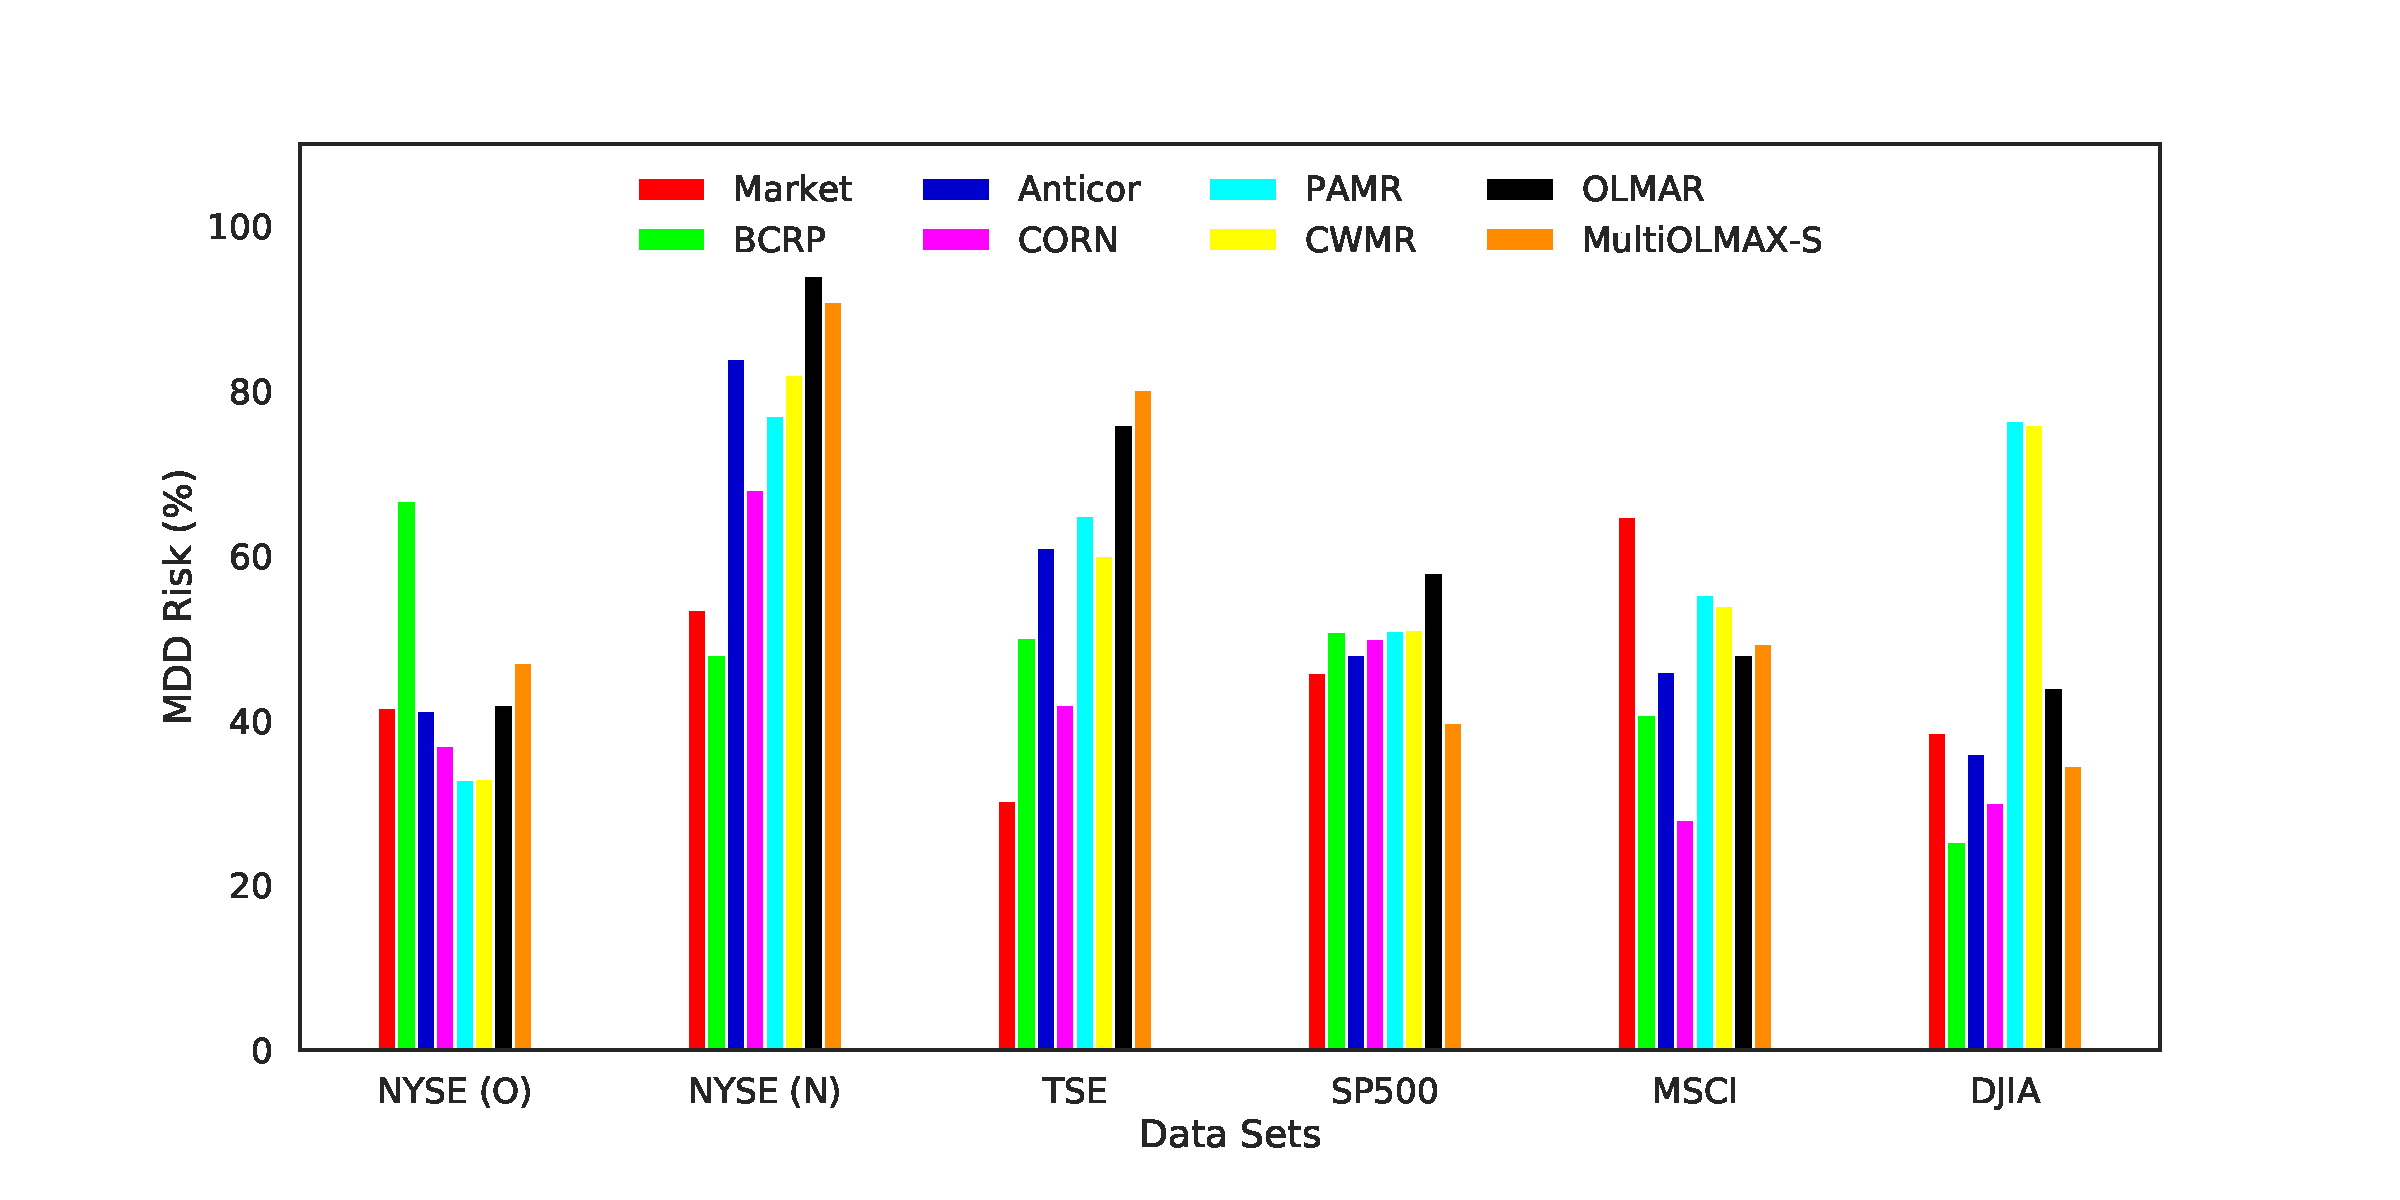
\includegraphics[width=\textwidth,height=\textheight,keepaspectratio]{mdds}%
}

\subfloat[Sharpe Ratio]{%
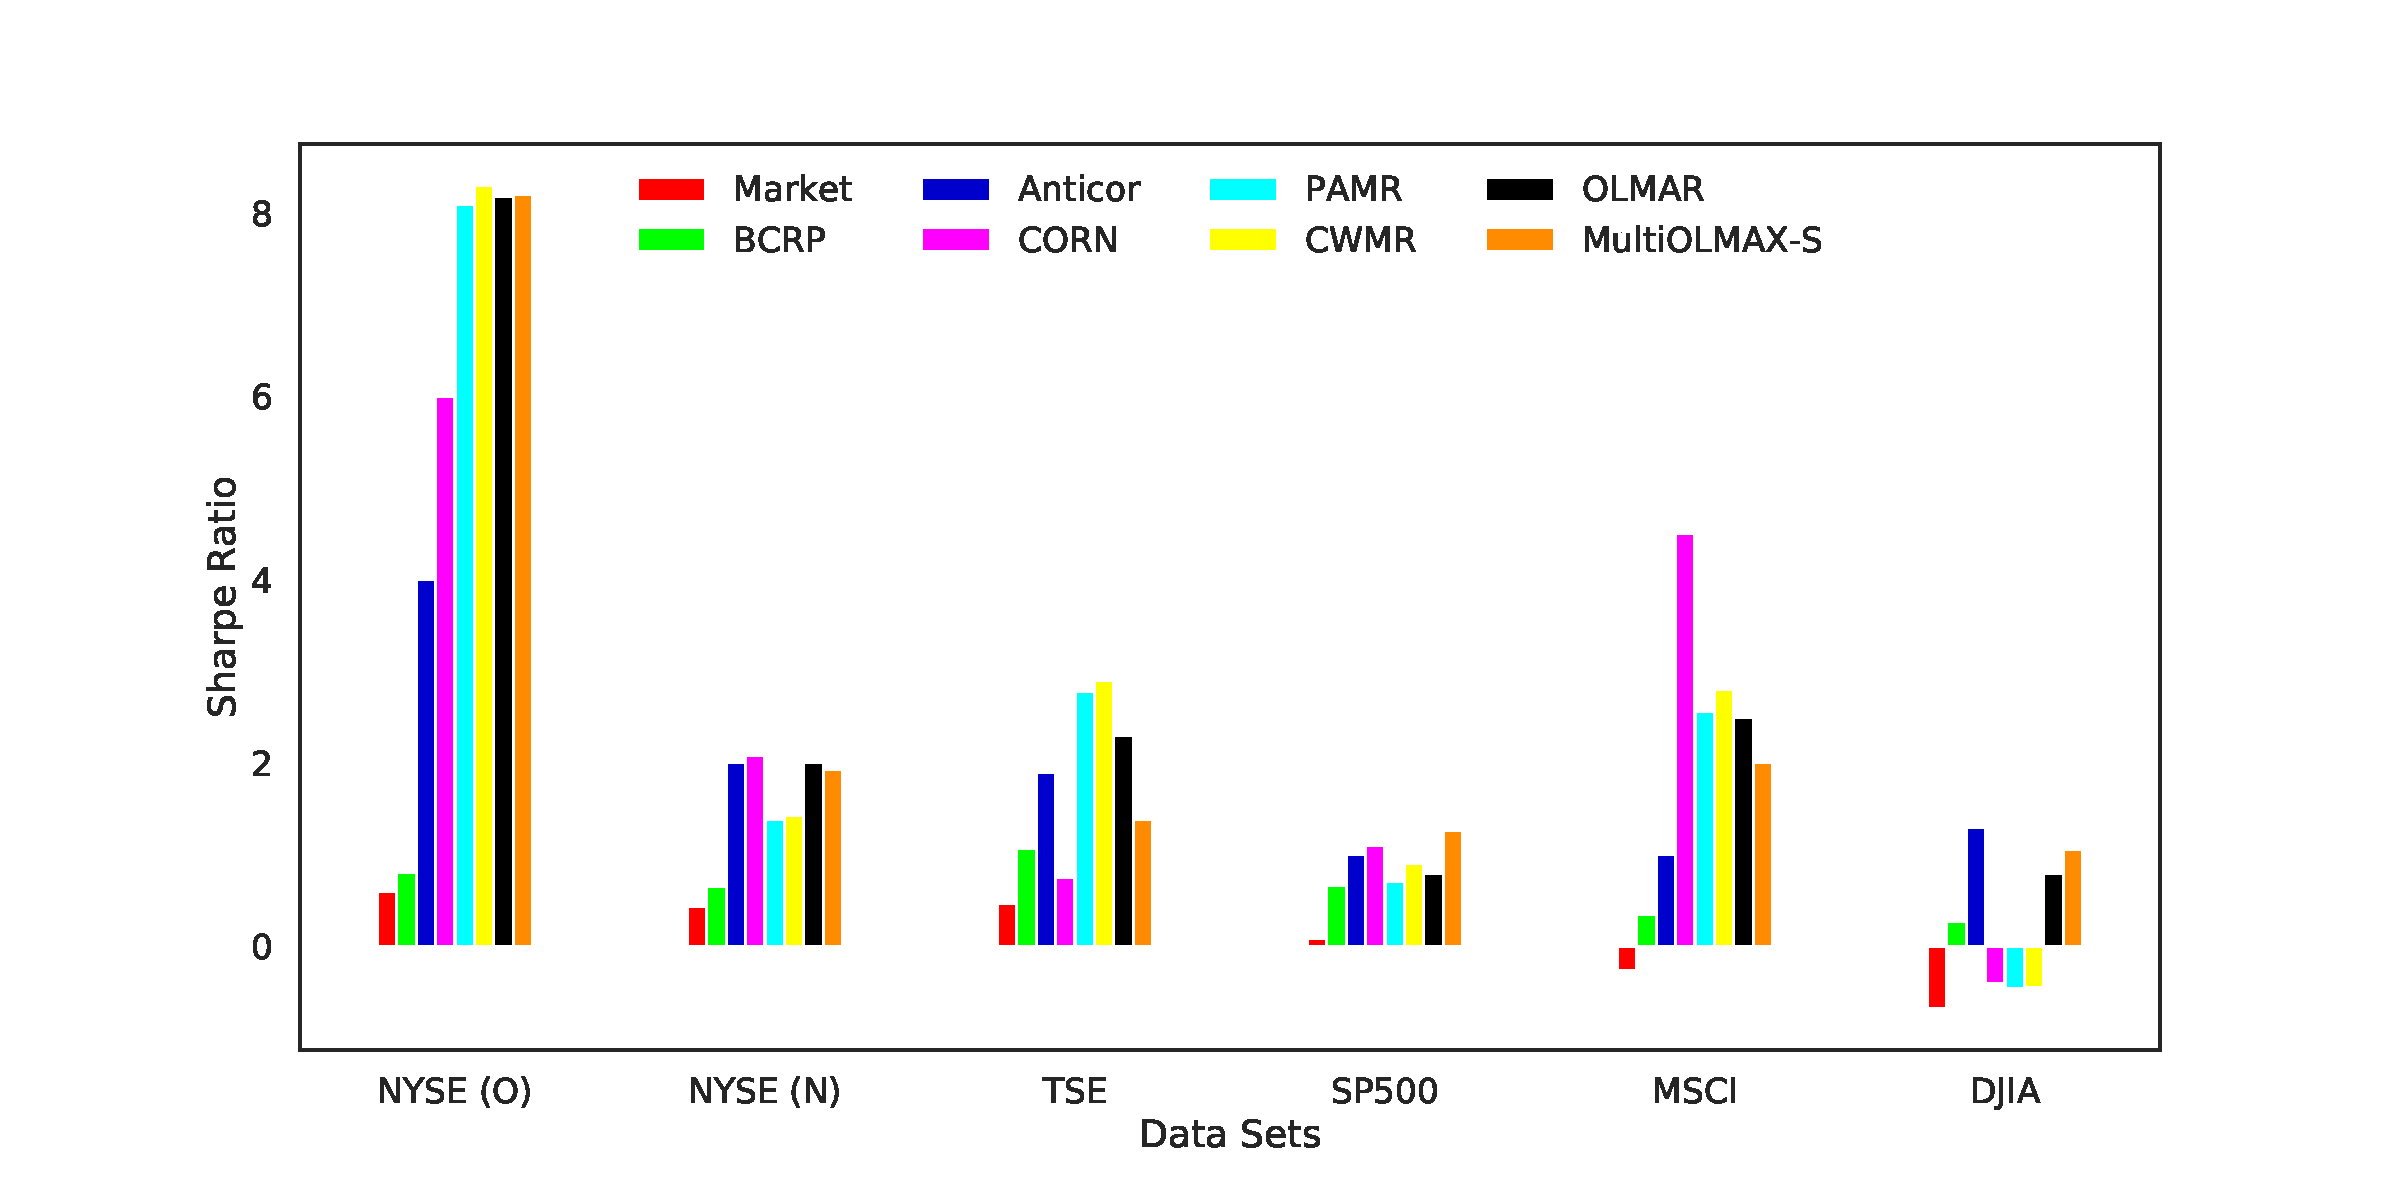
\includegraphics[width=\textwidth,height=\textheight,keepaspectratio]{sharpes}%
}
\end{figure}

\subsection{Hyperparameter sensitivity}
\label{sec:olmax-hyperparameter-sensitivity}

Next we assess the sensitivity of OLMAX with respect to its hyperparameters, namely the lookback window $w$ in the MultiOLMAX-S variant and the smoothing factor $\alpha$ in its MultiOLMAX-E counterpart. These are depicted in Figures~\ref{fig:multiolmax-sensitivity} and~\ref{fig:multiolmax2-sensitivity}, respectively.

From Figure~\ref{fig:multiolmax-sensitivity}, we see that as $w$ increases, the performance deteriorates on the NYSE (O), NYSE (N) and, following an initial spike, the MSCI data sets. As for TSE and SP500, MultiOLMAX-S attains the highest terminal wealth for $w = 35$ and $w = 65$, respectively, while on DJIA we observe a multi-modal pattern. It is remarkable that for most choices of $w$, the total wealth generated by MultiOLMAX-S exceeds that of the Market and BCRP benchmarks by a significant margin.

As for the MultiOLMAX-E variant, we observe in Figure~\ref{fig:multiolmax2-sensitivity} that on most data sets, terminal wealth is consistently high across a wide range of values for $\alpha$, the two extreme endpoints $\alpha = 0$ and $\alpha = 1$ being the exception. We can see why this is so, as follows. If $\alpha = 1$, then all expected price relatives are always 1 and MultiOLMAX-E outputs $\mathbf{b}_{t+1} = \mathbf{b}_t$ on each trading period $t$. Since, by convention, we use the equally-weighted portfolio $\mathbf{1}/m$ for initialisation purposes, this amounts to rebalancing the MultiOLMAX-E portfolio to the equally-weighted one on each trading period, which explains the poor performance. On the other hand, when $\alpha = 0$, the expected vector of price relatives equals $\widetilde{\mathbf{x}}_{t+1} = \frac{1}{\bigotimes_{\tau=1}^{t}\mathbf{x}}_{\tau}}$, i.e.\ it inversely relates to the entire history of price relatives, and should thereby not be expected to produce excellent results.

\begin{figure}%
\caption{Sensitivity of MultiOLMAX-S with respect to its lookback window $w$.}
\label{fig:multiolmax-sensitivity}
    \subfloat[NYSE (O)]{{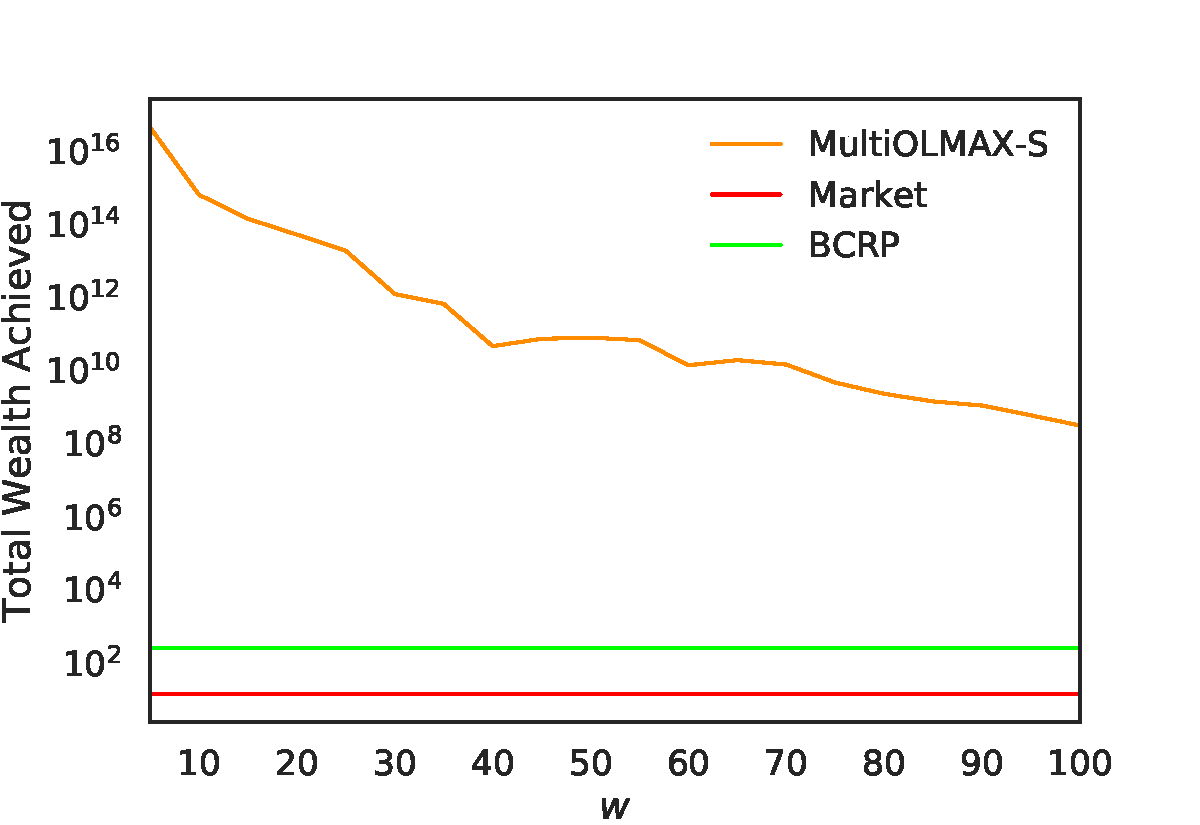
\includegraphics[width=4.5cm, keepaspectratio]{multiolmax-sensitivity_nyse-o} }}%
    \,
    \subfloat[NYSE (N)]{{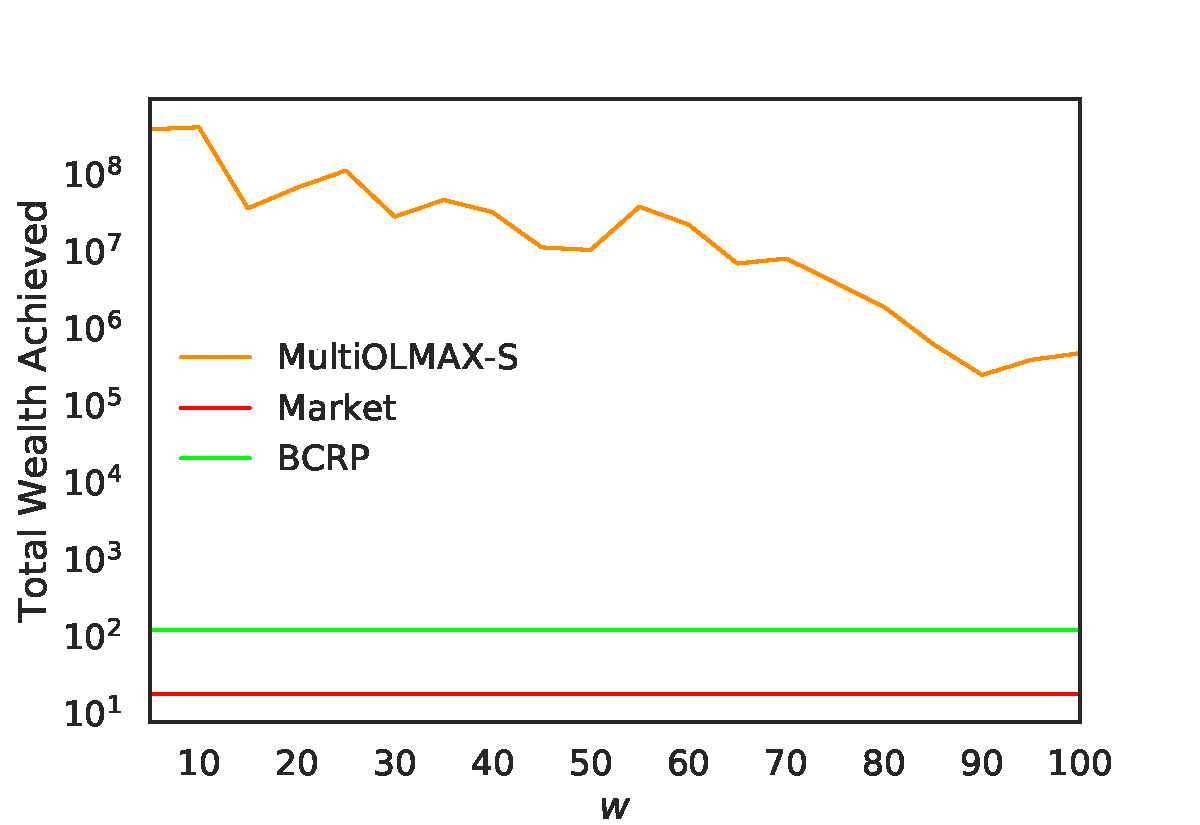
\includegraphics[width=4.5cm, keepaspectratio]{multiolmax-sensitivity_nyse-n} }}%
    \,
    \subfloat[TSE]{{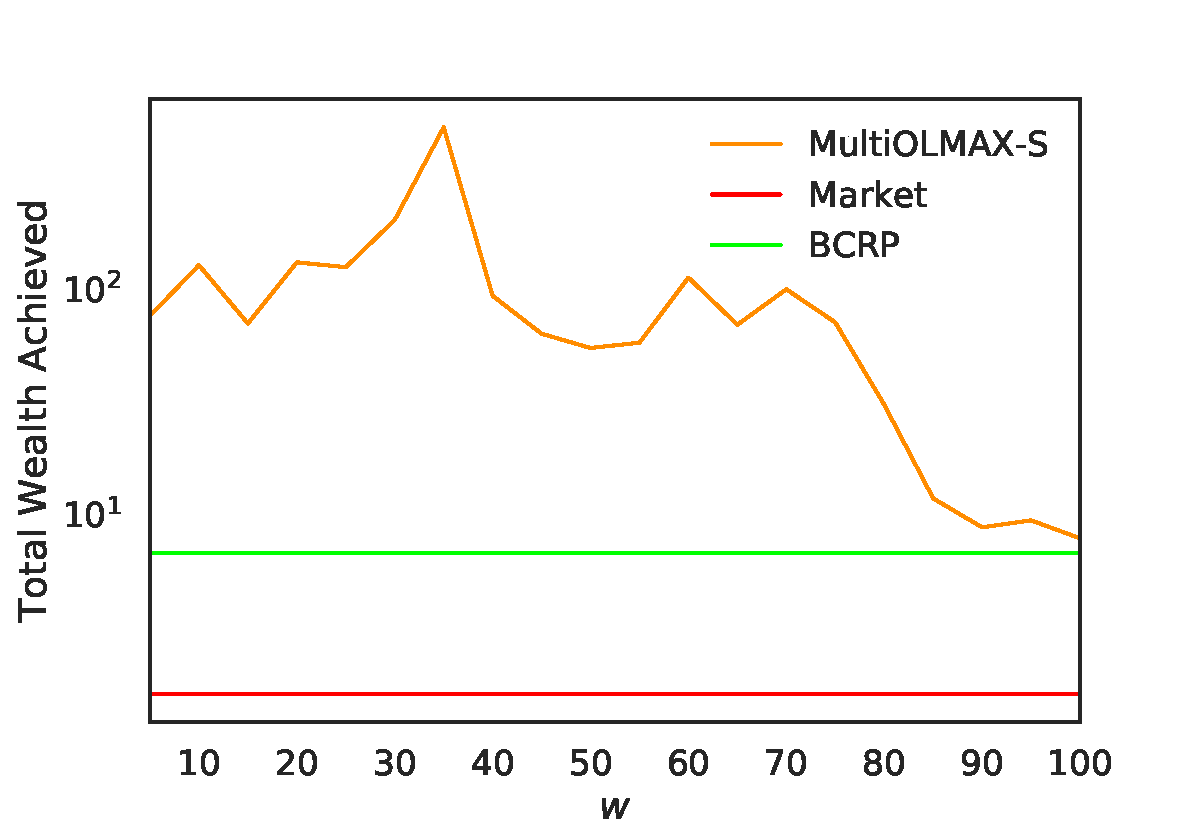
\includegraphics[width=4.5cm, keepaspectratio]{multiolmax-sensitivity_tse} }}%
    
    \subfloat[SP500]{{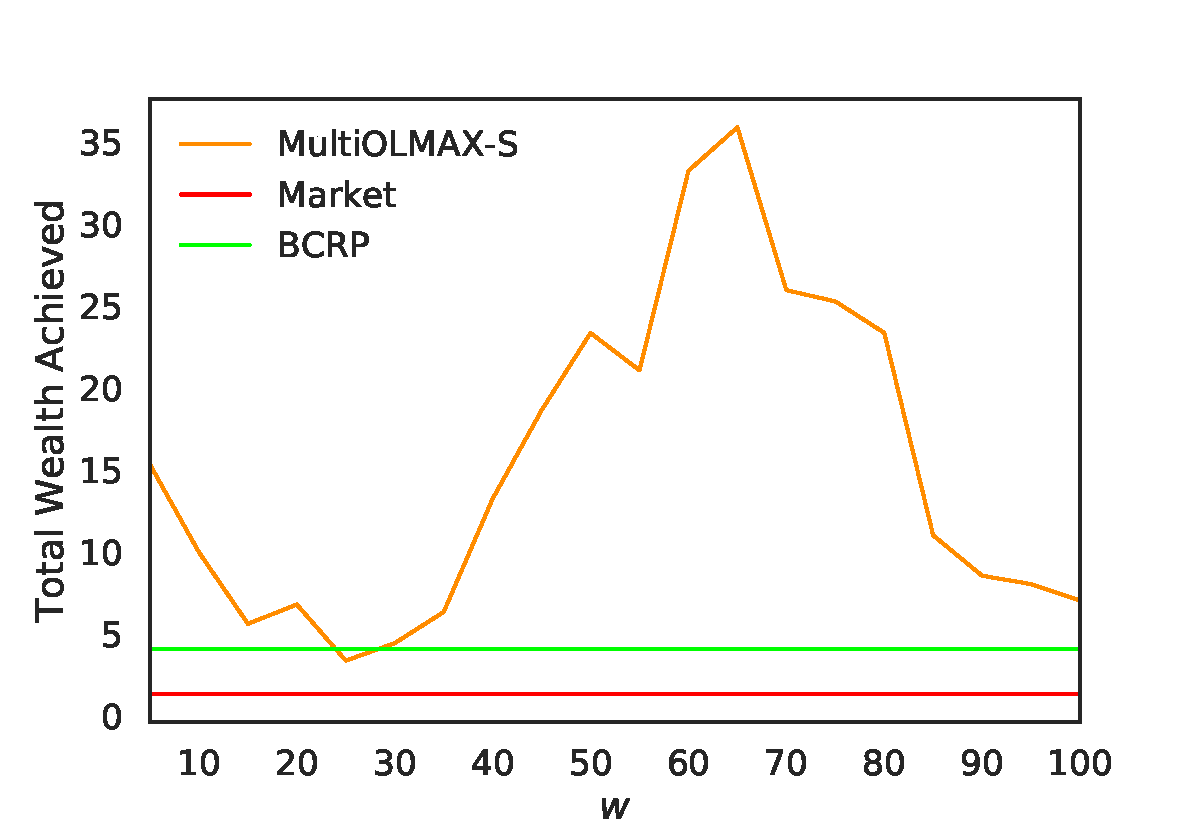
\includegraphics[width=4.5cm, keepaspectratio]{multiolmax-sensitivity_sp500} }}%
    \,
    \subfloat[MSCI]{{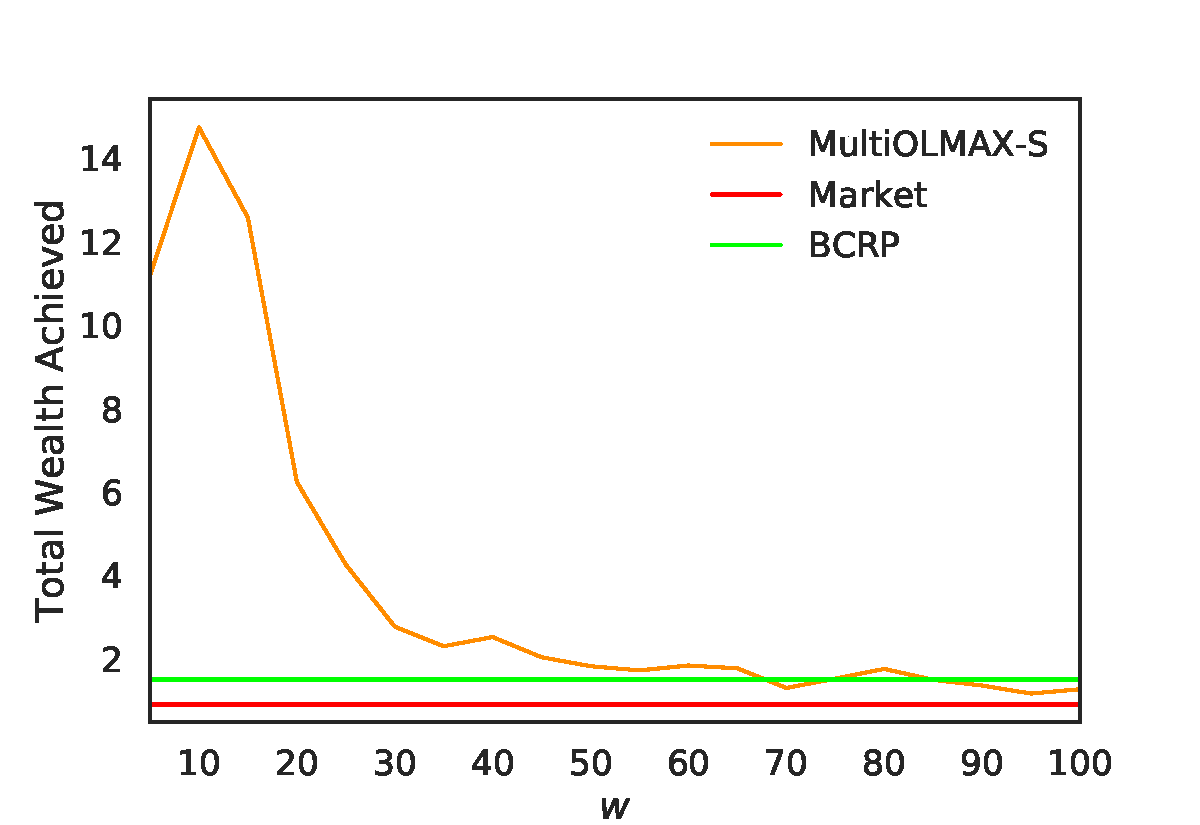
\includegraphics[width=4.5cm, keepaspectratio]{multiolmax-sensitivity_msci} }}%
    \,
    \subfloat[DJIA]{{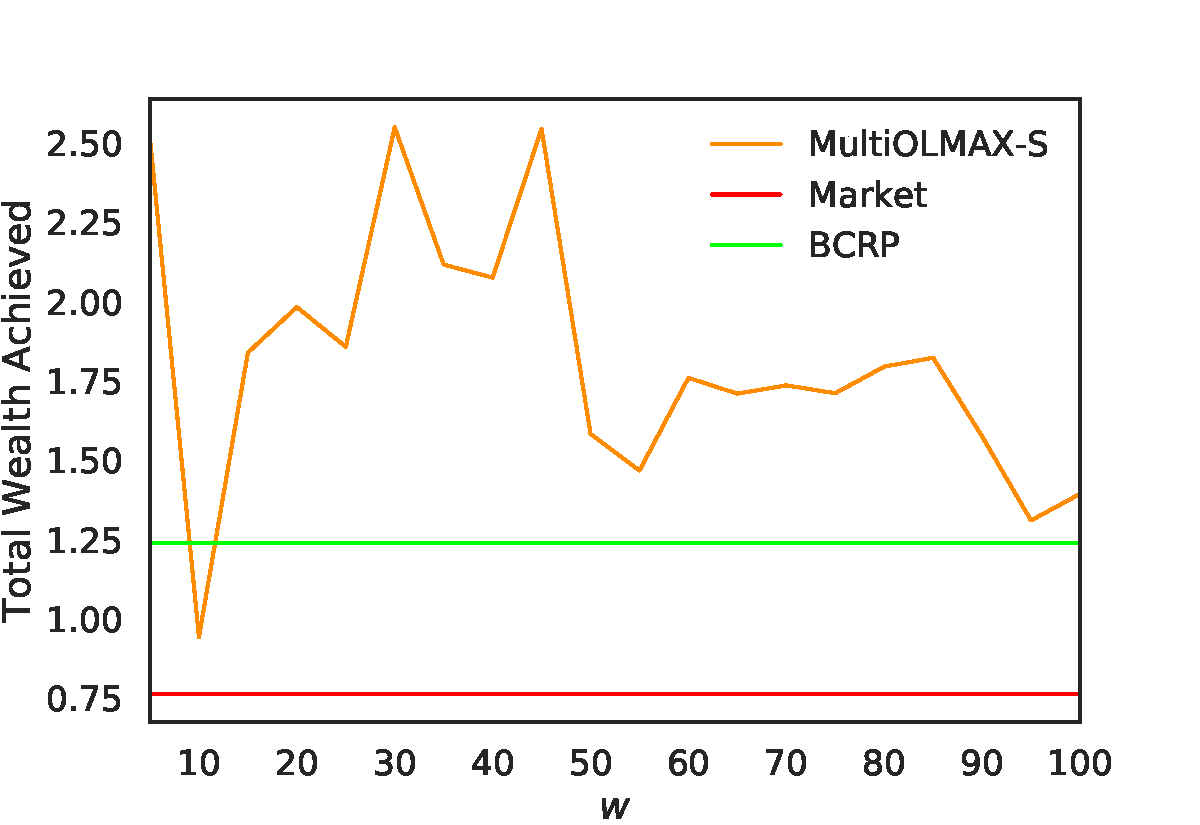
\includegraphics[width=4.5cm, keepaspectratio]{multiolmax-sensitivity_djia} }}%
\end{figure}

\begin{figure}%
\caption{Sensitivity of MultiOLMAX-E with respect to its smoothing factor $\alpha$.}
\label{fig:multiolmax2-sensitivity}
    \subfloat[NYSE (O)]{{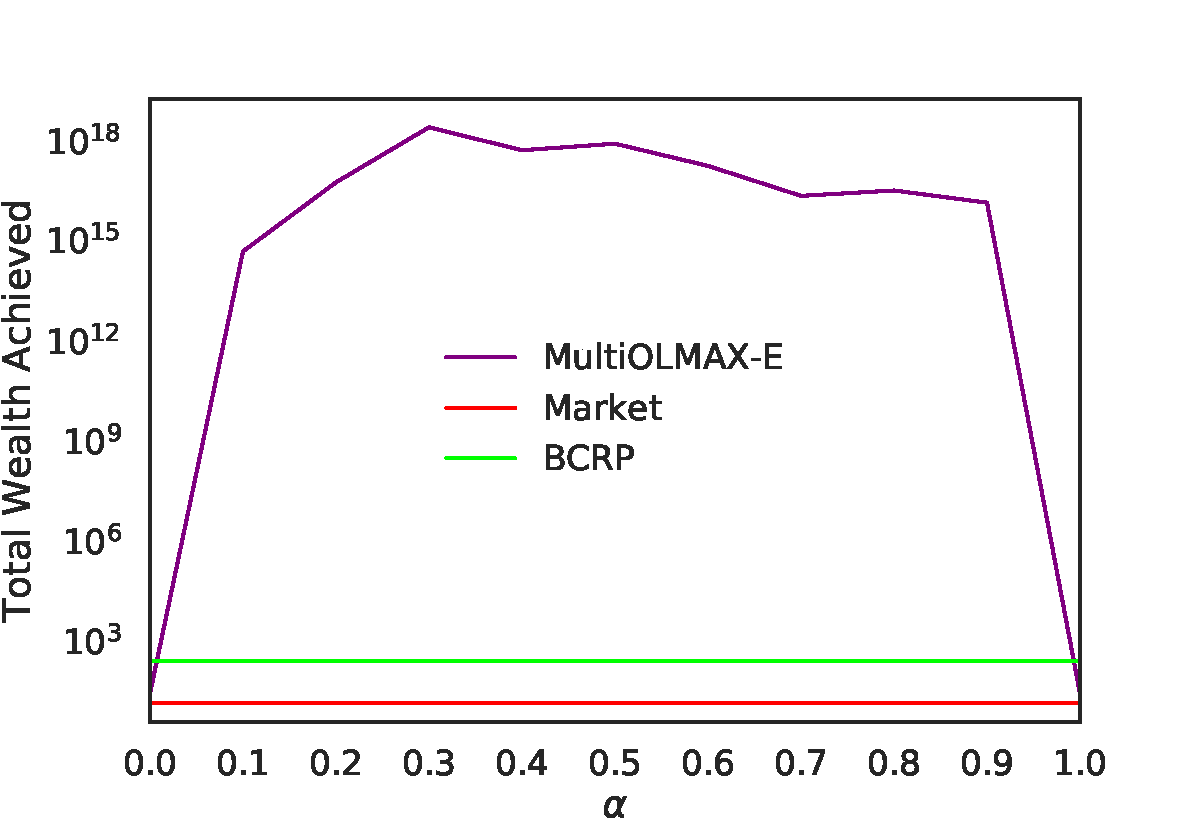
\includegraphics[width=4.5cm, keepaspectratio]{multiolmax2-sensitivity_nyse-o} }}%
    \,
    \subfloat[NYSE (N)]{{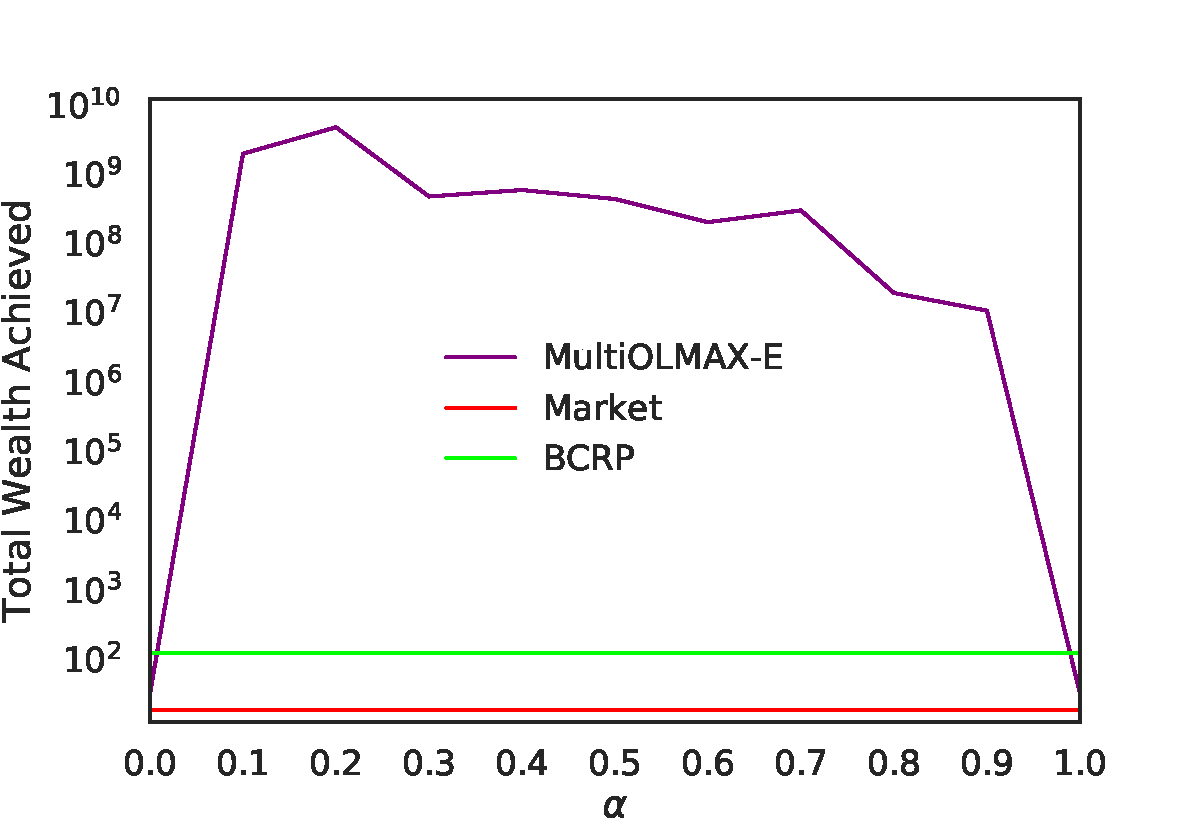
\includegraphics[width=4.5cm, keepaspectratio]{multiolmax2-sensitivity_nyse-n} }}%
    \,
    \subfloat[TSE]{{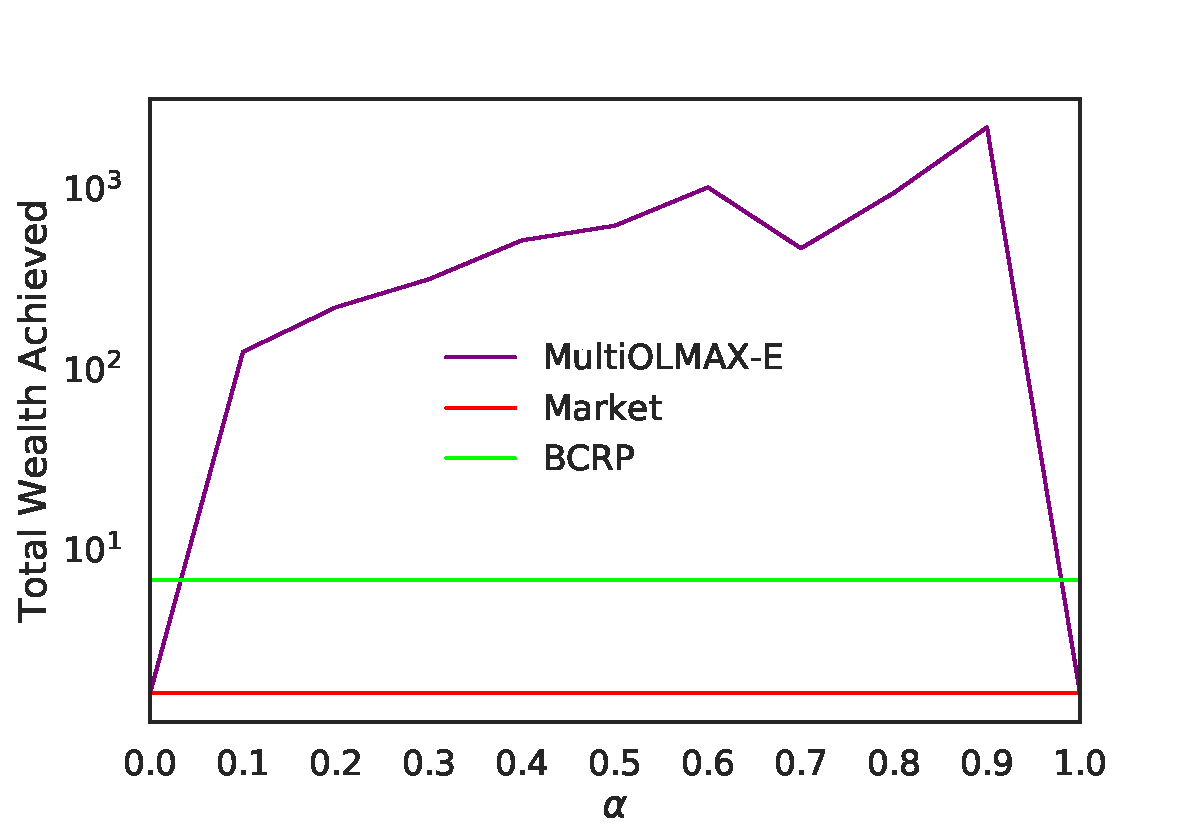
\includegraphics[width=4.5cm, keepaspectratio]{multiolmax2-sensitivity_tse} }}%
    
    \subfloat[SP500]{{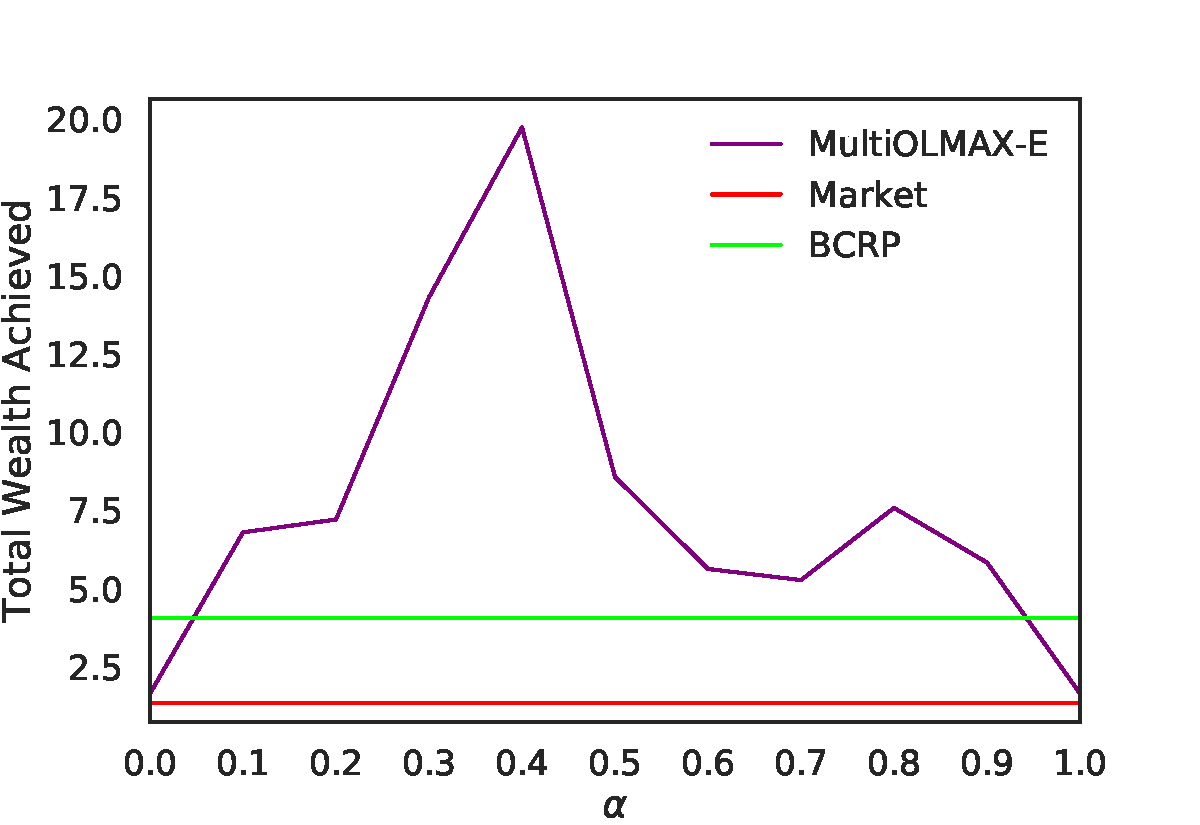
\includegraphics[width=4.5cm, keepaspectratio]{multiolmax2-sensitivity_sp500} }}%
    \,
    \subfloat[MSCI]{{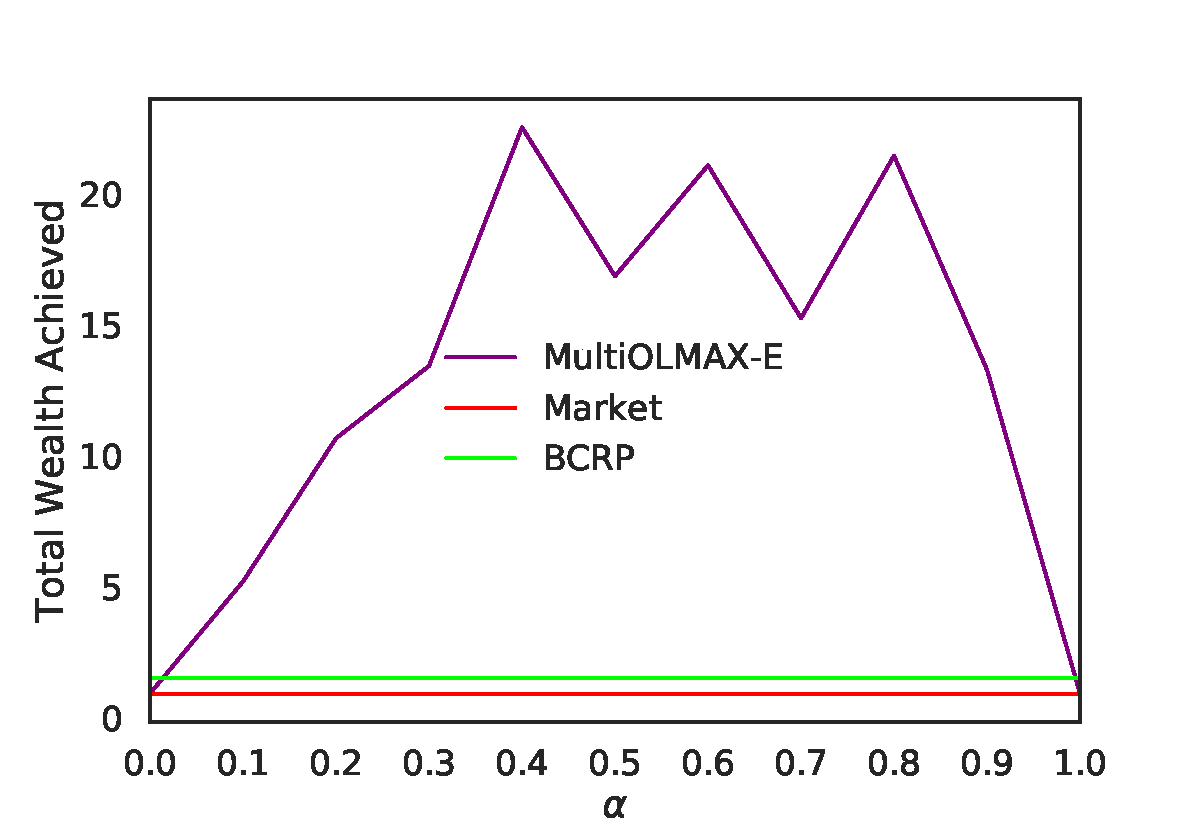
\includegraphics[width=4.5cm, keepaspectratio]{multiolmax2-sensitivity_msci} }}%
    \,
    \subfloat[DJIA]{{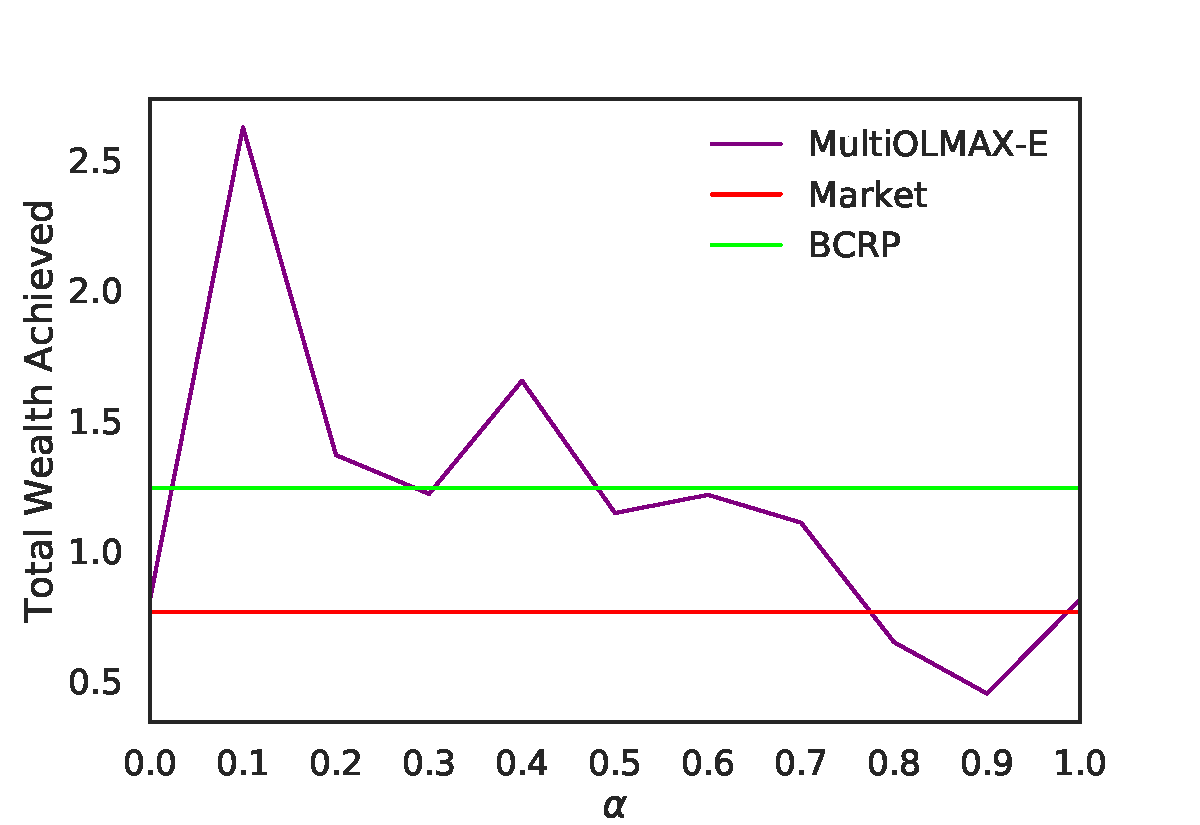
\includegraphics[width=4.5cm, keepaspectratio]{multiolmax2-sensitivity_djia} }}%
\end{figure}

\subsection{Practical performance under transaction costs}
\label{sec:transaction-costs}

To evaluate the practical applicability of the OLMAX framework, we analyse its robustness to proportional transaction fees \citep{borodin04}. Figure~\ref{fig:multiolmax-transaction-cost-sensitivity} illustrates the final wealth achieved by the MultiOLMAX-S method as a function of the transaction-cost rate $\gamma$, along with the corresponding results for the Market and BCRP benchmarks.
\begin{figure}%
\caption{Scalability of the proposed strategy with respect to the transaction-cost rate ($\gamma$).}
\label{fig:multiolmax-transaction-cost-sensitivity}
    \subfloat[NYSE (O)]{{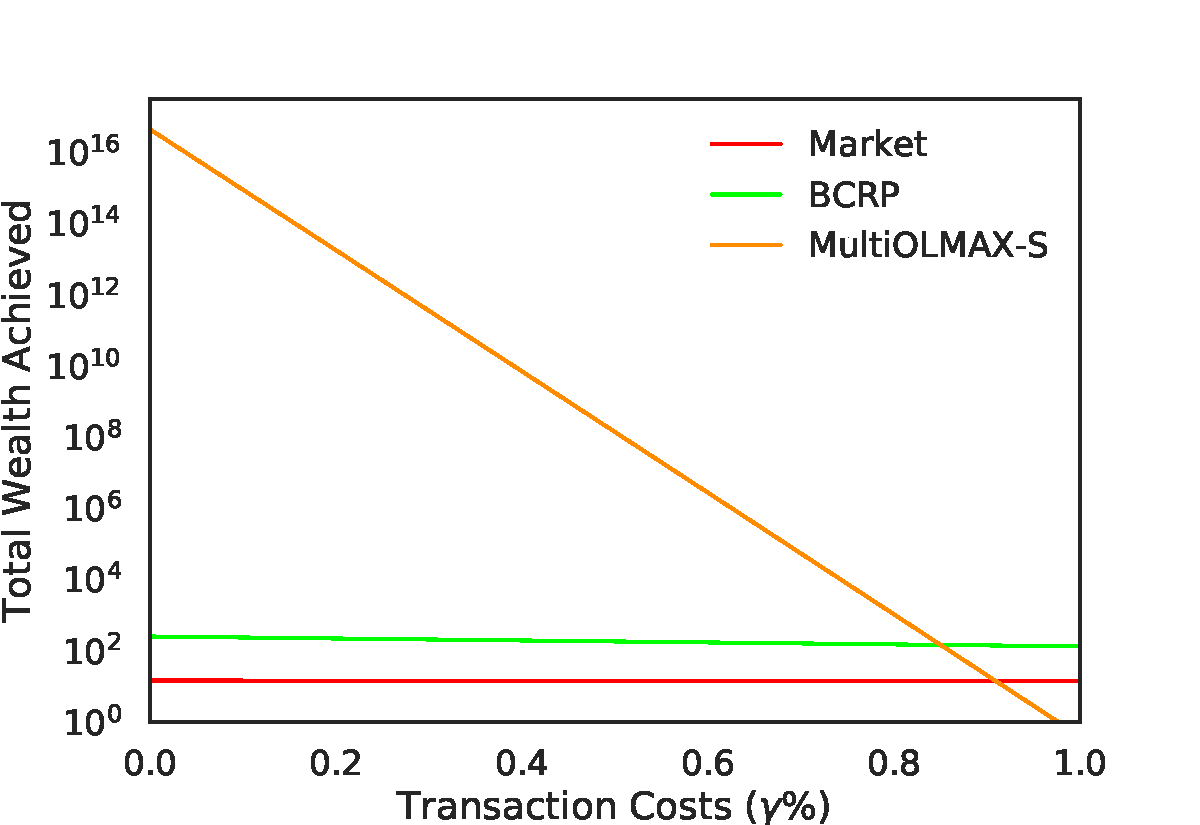
\includegraphics[width=4.5cm, keepaspectratio]{transaction-costs_nyse-o} }}%
    \,
    \subfloat[NYSE (N)]{{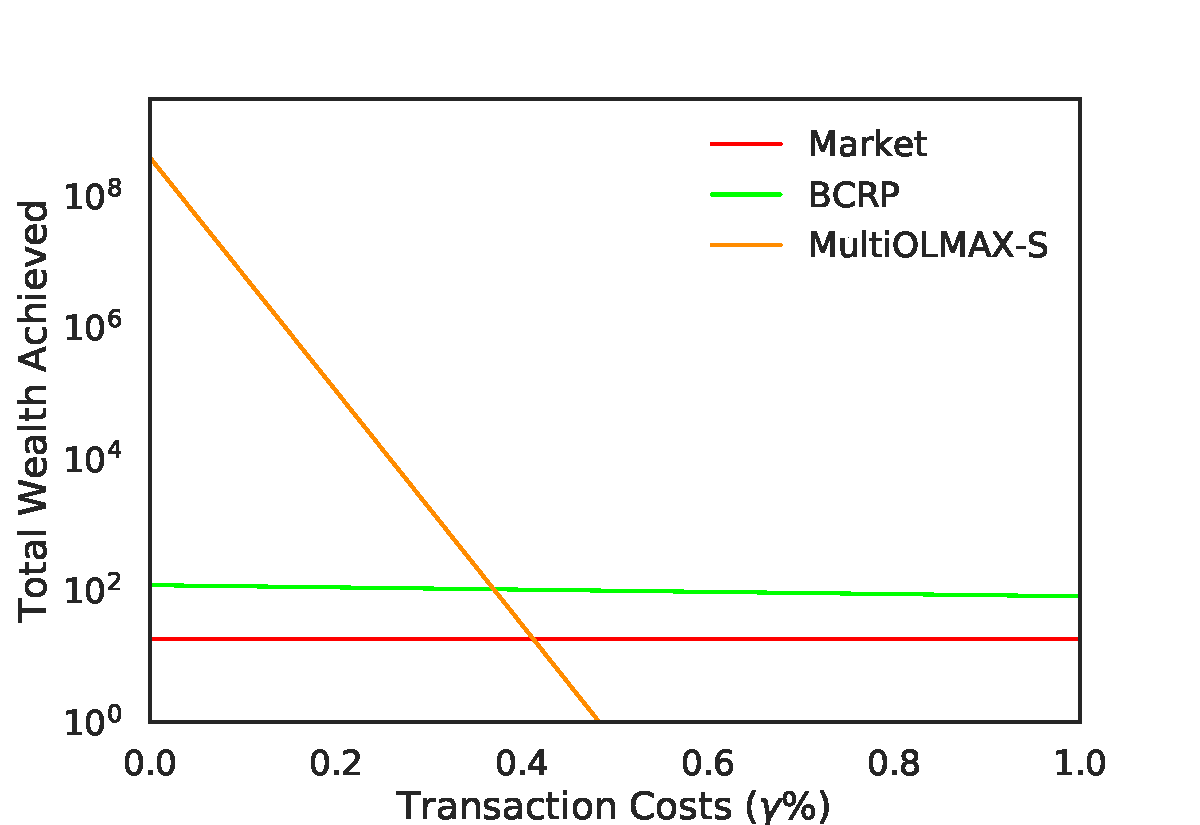
\includegraphics[width=4.5cm, keepaspectratio]{transaction-costs_nyse-n} }}%
    \,
    \subfloat[TSE]{{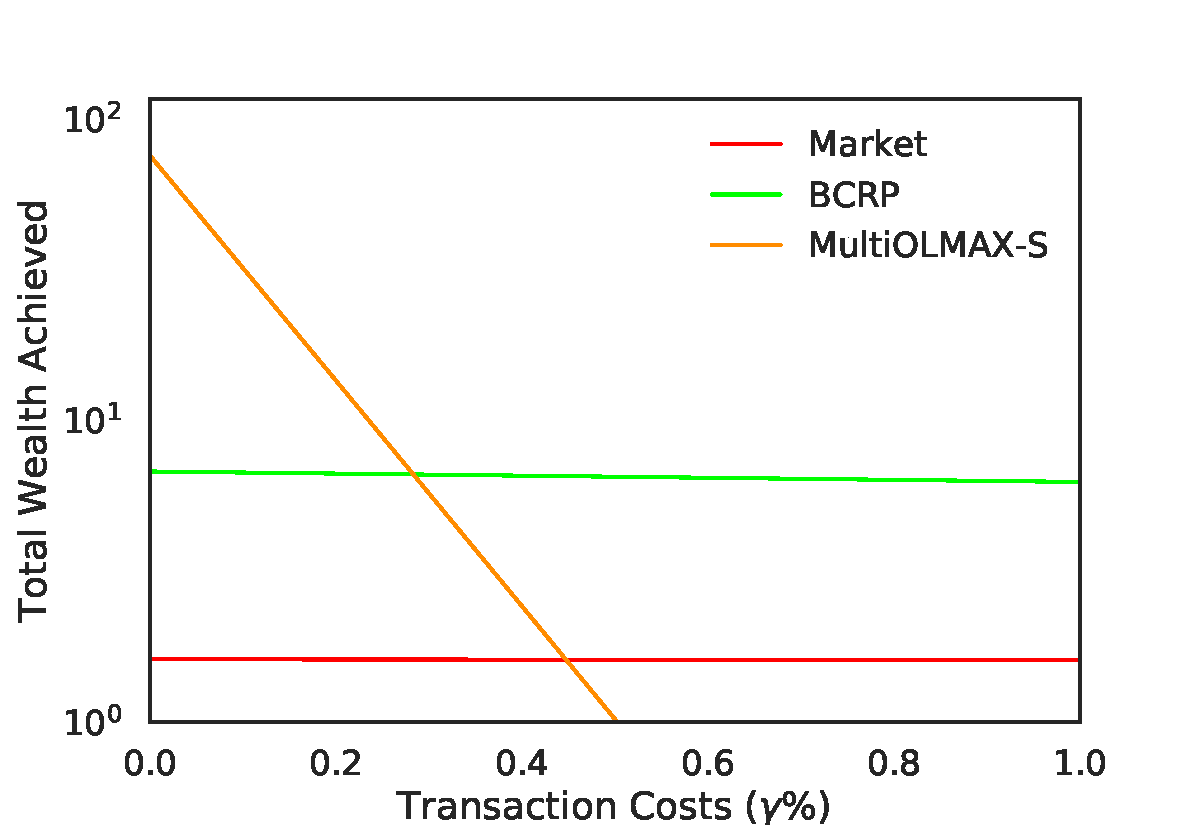
\includegraphics[width=4.5cm, keepaspectratio]{transaction-costs_tse} }}%
    
    \subfloat[SP500]{{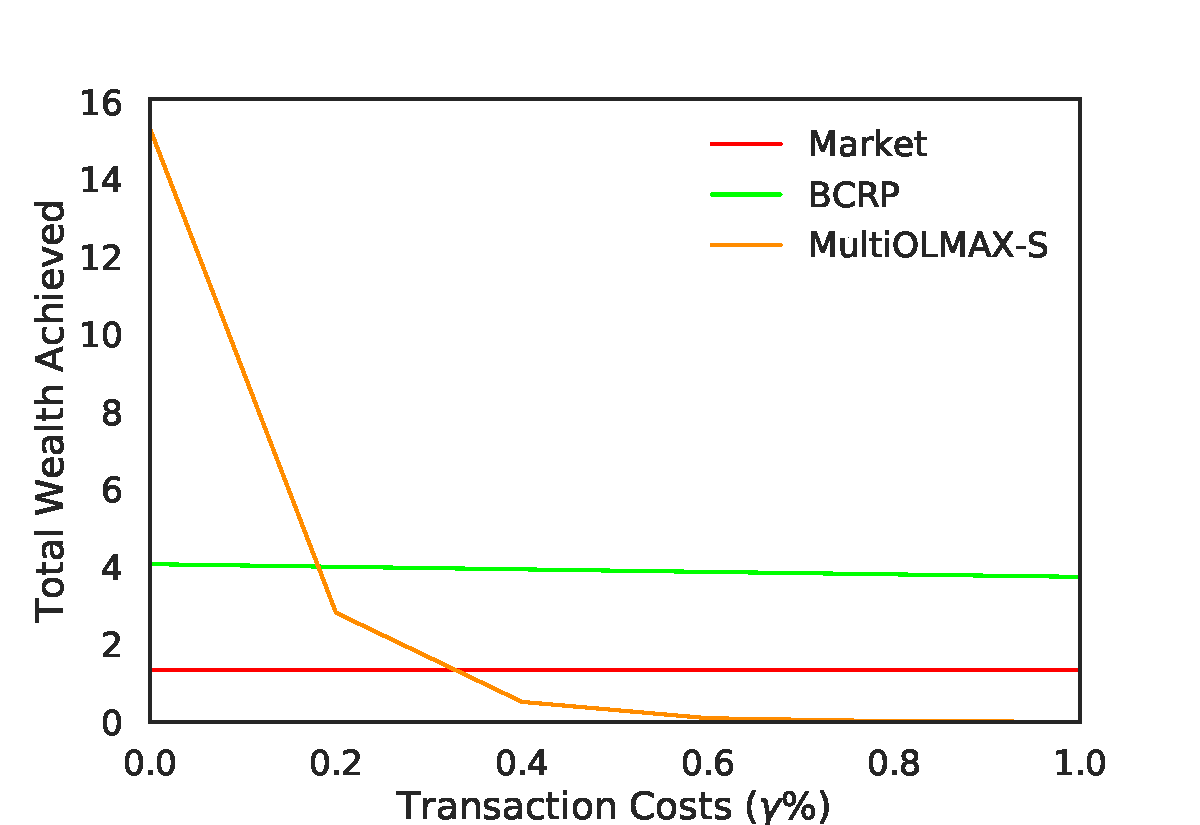
\includegraphics[width=4.5cm, keepaspectratio]{transaction-costs_sp500} }}%
    \,
    \subfloat[MSCI]{{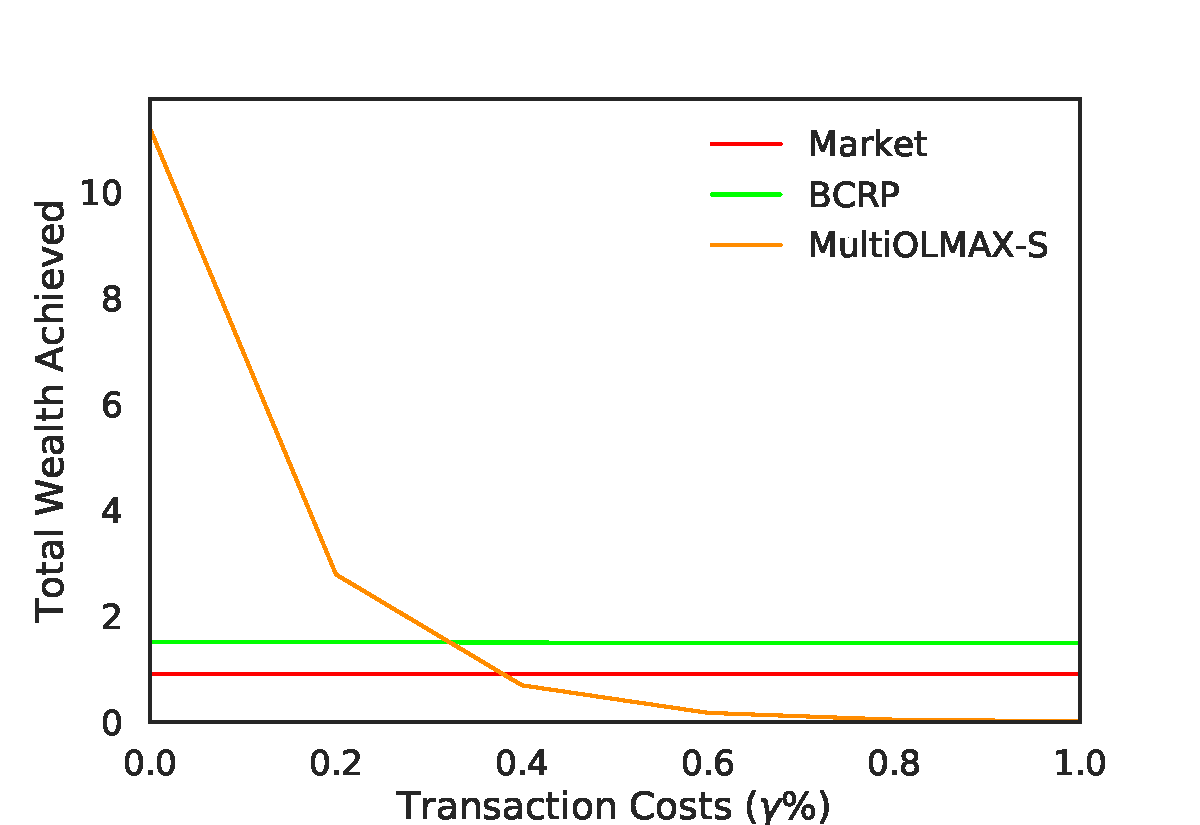
\includegraphics[width=4.5cm, keepaspectratio]{transaction-costs_msci} }}%
    \,
    \subfloat[DJIA]{{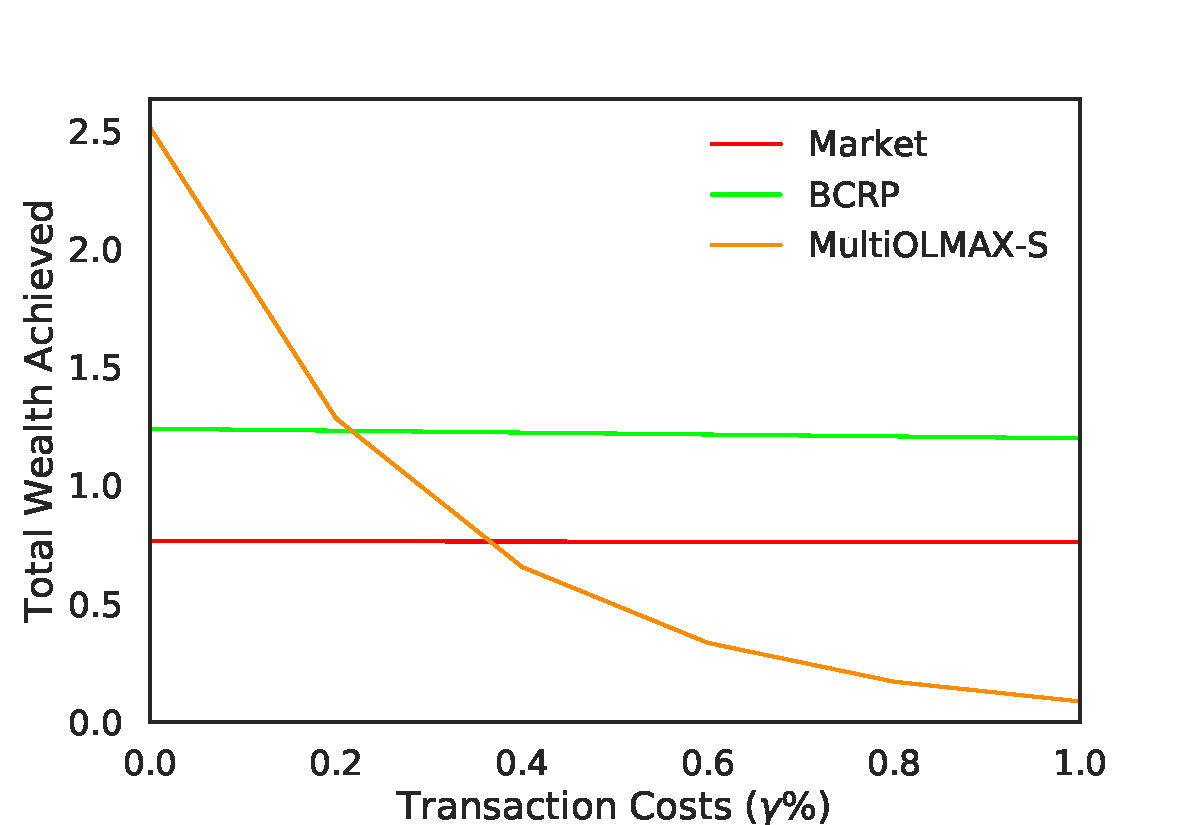
\includegraphics[width=4.5cm, keepaspectratio]{transaction-costs_djia} }}%
\end{figure}

On one hand, Figure~\ref{fig:multiolmax-transaction-cost-sensitivity} clearly shows that MultiOLMAX-S can withstand reasonable transaction costs, as it often has high break-even capability relative to the market. On the other hand, it can outperform the benchmarks under various transaction-cost assumptions. Consequently, MultiOLMAX-S exhibits outstanding performance even when trading is not frictionless, which provides further support to its practical applicability.

%\subsection{Evaluation of computational cost}

\section{Adaptive Online Mean Reversion}
\label{sec:ada-mr}

\subsection{Motivation}

Despite the effectiveness of the proposed OLMAX framework, one cannot help but notice that the corresponding experiments suffer from \emph{selection bias}, in the sense that they fail to cover asset classes other than equities. The same caveat holds for the CWMR, PAMR and OLMAR strategies, among others. The purpose of this subsection is to demonstrate that, in a portfolio that is broadly diversified in terms of asset classes, the aforementioned algorithms no longer exhibit a stellar performance after adding arguably reasonable fees of $0.1\%$ per transaction (corresponding to $\$1$ for every $\$1,000$ of bought/sold asset units). Additionally, we shall perform a sensitivity analysis suggesting that this practical limitation is related to the data-snooping bias from which these strategies suffer.

The first issue that we face concerns the best way to form a diversified portfolio. Since this lies outside the scope of this thesis, we shall simply follow the approach of David Swensen\footnote{David Swensen has been the chief investment officer of Yale University's endowment fund since 1985, and is highly regarded in the asset management community.}, who suggests a portfolio composed of six different asset classes, as follows: US equities (30\% weighting), international equities (15\%), emerging markets (10\%), Treasury inflation-protected securities (TIPS) (15\%), US treasuries (15\%) and real-estate investment trusts (REITs) (15\%) \citep{swensen}. Since we are not concerned with portfolio construction, we will use a set of highly liquid exchange-traded funds (ETFs) as vehicles for these asset classes. These are listed in Table~\ref{tab:etf-dataset}.
\begin{table}[H]
  \caption{Exchange-traded fund (ETF) dataset used in our empirical evaluation. Daily adjusted closing prices for these ETFs were obtained from \href{https://finance.yahoo.com/}{Yahoo! Finance}, for the period from January 1, 2005 until June 3, 2019 inclusive.}
  \label{tab:etf-dataset}
  \centering
  \resizebox{\textwidth}{!}{\begin{tabular}{llccc}
    \toprule
    Ticker & Name & Asset Class & Region & Number of Holdings \\
    \midrule
    VTI & Vanguard Total Stock Market ETF & Equity & US & 3629 \\
    EFA & iShares MSCI EAFE ETF & Equity & Europe, Australia, Asia \& the Far East & 937 \\
    EEM & iShares MSCI Emerging Markets ETF & Equity & Emerging markets & 857 \\
    TLT & iShares 20+ Year Treasury Bond ETF & Fixed Income & US & 30 \\
    TIP & iShares TIPS Bond ETF & Fixed Income & US & 38 \\
    VNQ & Vanguard Real Estate ETF & Equity & US & 184 \\
    \bottomrule
\end{tabular}}
\end{table}

Figure~\ref{fig:etf-cumwealth} clearly illustrates the lack of robustness with respect to transaction costs of PAMR, CWMR, OLMAR, SingleOLMAX and MultiOLMAX\footnote{Henceforth, the acronym `MultiOLMAX' will be used as a shorthand for the MultiOLMAX-S strategy, whose price-relative forecasts are based on simple moving averages.}. Under the absence of transaction costs, these methods exhibit decent performance in terms of cumulative wealth, and even exceed the benchmarks (including Swensen's recommended portfolio) by a highly significant margin. However, the picture changes drastically when one introduces fees of 0.1\% per transaction, and none of these algorithms manages to beat any of the benchmarks. Worse, they all stagnate around 2010 and their performance starts deteriorating in 2011 or a couple of years thereafter.
\begin{figure}[H]
    \subfloat[Without fees]{{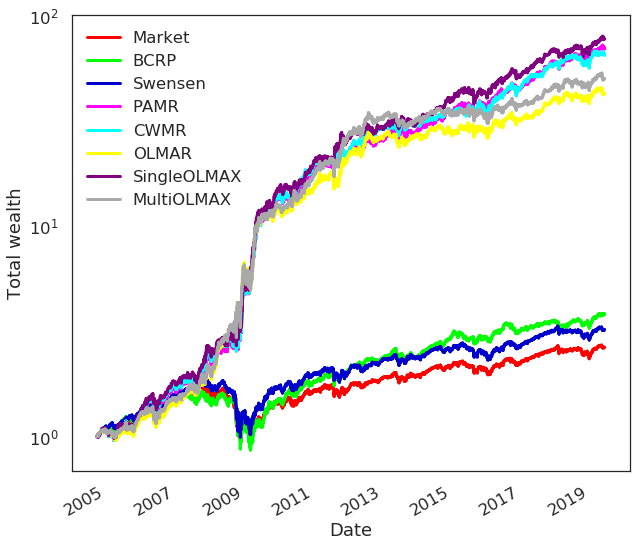
\includegraphics[width=0.5\textwidth, keepaspectratio]{etf-cumwealth-no-fees} }}%
    \,
    \subfloat[Subject to fees of 0.1\%]{{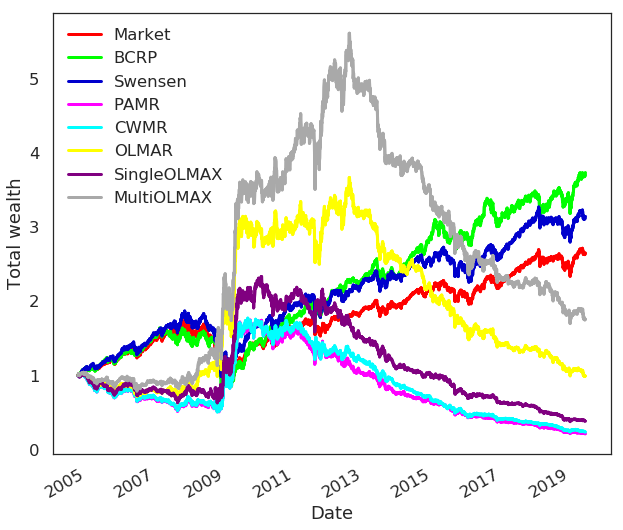
\includegraphics[width=0.5\textwidth, keepaspectratio]{etf-cumwealth-with-fees} }}%
\caption{Trends of cumulative wealth achieved by various strategies during the entire trading periods associated with the ETF data set (see Table~\ref{tab:etf-dataset}). Panel \textbf{(a)} illustrates these trends under the assumption of no transaction costs, whereas panel \textbf{(b)} depicts them net of fees of 0.1\% per transaction.}
\label{fig:etf-cumwealth}
\end{figure}

A deeper analysis reveals that the underperformance documented above may be due to data-snooping bias. Let us focus on OLMAR, for the sake of argument. In Figure~\ref{fig:olmar-sensitivity}, we see with hindsight that the optimal terminal wealth does not occur at the default values $\epsilon = 10$ and $w = 5$ of the underlying parameters, where, as a reminder, $\epsilon$ is the reversion threshold and $w$ the lookback window used in the computation of the price-relative forecasts. For instance, if we keep $\epsilon$ fixed at 10, the optimal window yielding the highest final wealth is $w = 20$. Once we implement the OLMAR algorithm with these parameter values optimised with the benefit of hindsight, we are able to improve its \emph{net} performance (i.e.\ net of transaction fees) beyond that of the benchmarks, as illustrated in Figure~\ref{fig:optimised-olmar}.

\begin{figure}[H]
\caption{Parameter sensitivity of OLMAR on the ETF data set, with respect to \textbf{(a)} $\epsilon$ with fixed $w$ ($w = 5$) and \textbf{(b)} $w$ with fixed $\epsilon$ ($\epsilon = 10$).}
\label{fig:olmar-sensitivity}
    \subfloat[]{{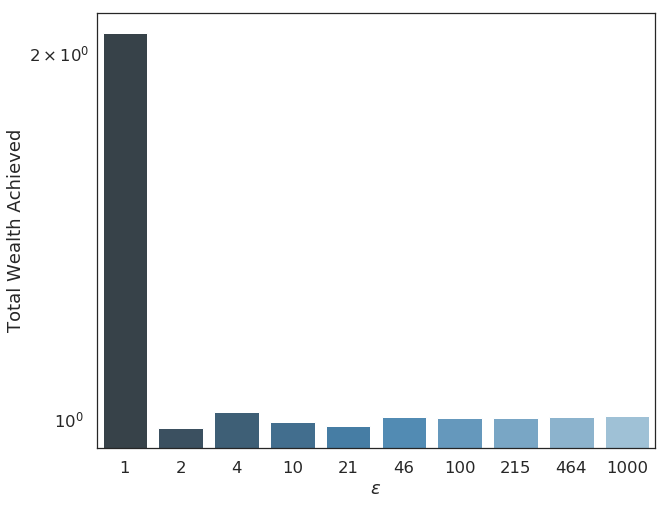
\includegraphics[width=0.5\textwidth, keepaspectratio]{olmar-sensitivity-epsilon_etfs} }}%
    \subfloat[]{{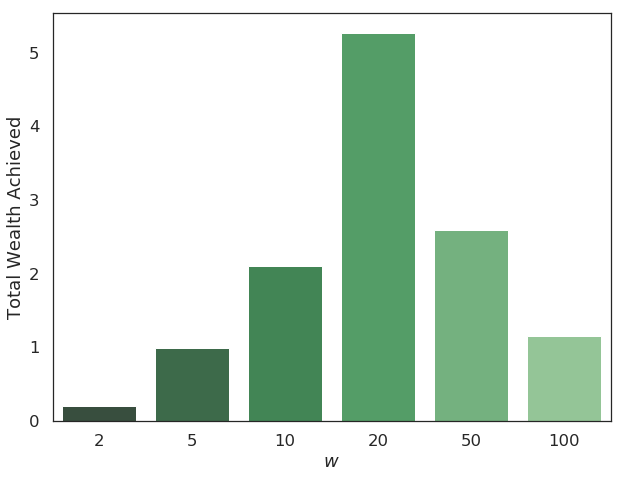
\includegraphics[width=0.5\textwidth, keepaspectratio]{olmar-sensitivity-window_etfs} }}%
\end{figure}

\begin{figure}[H]
\centering
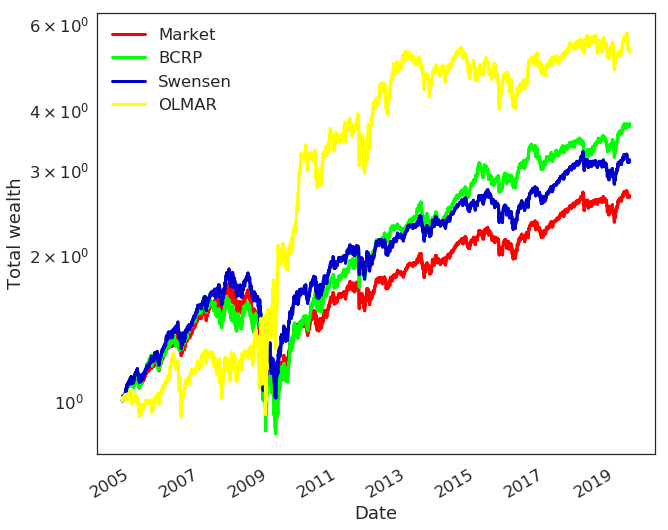
\includegraphics[width=\textwidth, height=\textheight, keepaspectratio]{etf-cumwealth-optolmar-with-fees}
\caption{Cumulative wealth achieved by OLMAR optimised in hindsight (with parameters $\epsilon = 10$ and $w = 20$) vs benchmarks on the ETF data set, subject to transaction fees of 0.1\%.}
\label{fig:optimised-olmar}
\end{figure}

\subsection{Proposed algorithms}

Armed with the insights from Figures~\ref{fig:olmar-sensitivity} and~\ref{fig:optimised-olmar}, we turn now to explore \emph{adaptive} variants of PAMR and OLMAR that are governed by no and a smaller number of hyperparameters, respectively. To this end, we cast the underlying optimisation problems into a, roughly speaking, equivalent OGD-criterion representation (see Eq. \eqref{eq:ogd-criterion}) whose learning rate can be made adaptive via the application of the MAPGRAD algorithm (i.e.\ Algorithm~\ref{alg:mapgrad}).

To start with, let us consider the PAMR strategy. As proposed in \citep{pamr}, the standard variant is formulated as the following constrained optimisation problem:
\begin{equation}
\label{eq:pamr-optpb}
	\min_{\mathbf{b}\in\Delta_m} \; \frac{1}{2}\Vert\mathbf{b} - \mathbf{b}_t\Vert_2^2
	\qquad \text{s.t.} \qquad \mathbf{b} \cdot \mathbf{x}_t \leq \epsilon,
\end{equation}
for $t \in [T-1]$, with the convention $\mathbf{b}_1 = \mathbf{1} / m$. Instead of this problem, we will consider the following proximal problem:
\begin{equation}
\label{eq:pamr-optpb-ogdform}
	\min_{\mathbf{b}\in\Delta_m} \; \Big\{\eta(\mathbf{b} \cdot \mathbf{x}_t) + \frac{1}{2}\Vert\mathbf{b} - \mathbf{b}_t\Vert_2^2\Big\}
	= \min_{\mathbf{b}\in\Delta_m} \; \Big\{\mathbf{b} \cdot \mathbf{x}_t + \frac{1}{2\eta}\Vert\mathbf{b} - \mathbf{b}_t\Vert_2^2\Big\},
\end{equation}
for some $\eta > 0$.
Roughly speaking, the PAMR problem \eqref{eq:pamr-optpb} and the proximal problem \eqref{eq:pamr-optpb-ogdform} have the same solutions for appropriate choices of the parameters $\epsilon$ and $\eta$.
%More precisely, every solution of the proximal problem \eqref{eq:pamr-optpb-ogdform} is also a solution of the PAMR problem \eqref{eq:pamr-optpb} for some choice of $\epsilon$. Conversely, every solution of the PAMR problem \eqref{eq:pamr-optpb} is either a minimiser of
However, the formulation \eqref{eq:pamr-optpb-ogdform} has the form of the OGD criterion in Eq. \eqref{eq:ogd-criterion}, meaning the portfolio weights that solve \eqref{eq:pamr-optpb-ogdform} satisfy the OGD update rule \eqref{eq:ogd}:
\begin{equation}
\label{eq:pamr-portfolio}
	\mathbf{b}_{t+1} = \Pi_{\Delta_m}(\mathbf{b}_t - \eta\mathbf{x}_t),
\end{equation}
where, as a reminder, $\Pi_{\Delta_m}(\mathbf{b})$ signifies the point in $\Delta_m$ that is closest to $\mathbf{b}$.
In order to marginalise the dependence on $\eta$ of the portfolio updates in Eq. \eqref{eq:pamr-portfolio}, we employ the MAPGRAD method outlined in Algorithm~\ref{alg:mapgrad}. The latter prescribes the data-dependent learning-rate schedule $\{\eta_t = m / \Vert\sum_{\tau=1}^{t}\mathbf{x}_\tau\Vert^2_2\,\}_{t=1}^{T-1}$ which, when plugged into Eq. \eqref{eq:pamr-portfolio}, yields the strategy
\begin{equation}
\label{eq:adapamr-portfolio}
	\mathbf{b}_{t+1}
	= \Pi_{\Delta_m}\left(\mathbf{b}_t - \frac{m}{\Vert\sum_{\tau=1}^{t}\mathbf{x}_\tau\Vert^2_2}\,\mathbf{x}_t\right),
	\qquad t \in [T-1],
\end{equation}
subject to the initialisation condition $\mathbf{b}_1 = \mathbf{1} / m$.
For obvious reasons, we shall refer to the latter as \emph{adaptive passive-aggressive mean reversion} strategy, or AdaPAMR for short. The procedure is outlined in Algorithm~\ref{alg:adapamr}.
\begin{algorithm}
  \caption{AdaPAMR: Adaptive Passive-Aggressive Mean Reversion}
\label{alg:adapamr}
  \begin{algorithmic}[1]
    \STATE {\bfseries Initialisation:} initial portfolio $\mathbf{b}_1 = \frac{\mathbf{1}}{m}$, initial wealth $S_0 = 1$, initial gradient sum $\boldsymbol{\theta}_0 = \mathbf{0}$
    \FOR{$t=1, 2, \ldots, T$}
      \STATE observe stock price relatives $\mathbf{x}_t$
      \STATE update wealth:
        $
          S_t = S_{t-1} \times (\mathbf{b}_t^\text{T}\mathbf{x}_t)
        $
      \IF {$t < T$}
        \STATE update the gradient sum: $\boldsymbol{\theta}_t = \boldsymbol{\theta}_{t-1} + \mathbf{x}_t$
        \STATE compute the learning rate:
        \begin{equation*}
        	\eta_t = \frac{m}{\Vert\boldsymbol{\theta}_{t}\Vert^2_2}
        \end{equation*}
        \STATE update the portfolio:
	\begin{equation*}
		\mathbf{b}_{t+1} = 	\mathbf{b}_{t} - \eta_t\mathbf{x}_t
	\end{equation*}
		\STATE normalise the portfolio:
		\begin{equation*}
			\mathbf{b}_{t+1} = \Pi_{\Delta_m}(\mathbf{b}_{t+1})
			= \argmin_{\mathbf{b}\in\Delta_m} \; \Vert\mathbf{b} - \mathbf{b}_{t+1}\Vert_2^2
		\end{equation*}
	\ENDIF
    \ENDFOR
  \end{algorithmic}
\end{algorithm}

The derivation of the adaptive OLMAR (AdaOLMAR) algorithm is similar, so our exposition thereof will be brief. We replace the OLMAR optimisation problem
\begin{equation}
\label{eq:olmar-optpb}
	\min_{\mathbf{b}\in\Delta_m} \; \frac{1}{2}\Vert\mathbf{b} - \mathbf{b}_t\Vert_2^2
	\qquad \text{s.t.} \qquad \mathbf{b} \cdot \widetilde{\mathbf{x}}_{t+1} \geq \epsilon
\end{equation}
with the proximal problem\footnote{Note the negative sign preceding the loss term $\mathbf{b} \cdot \widetilde{\mathbf{x}}_{t+1}$. This is required because OLMAR's key constraint is $\mathbf{b} \cdot \widetilde{\mathbf{x}}_{t+1} \geq \epsilon$, i.e.\ it has a \emph{greater-or-equal} sign, unlike PAMR's key constraint $\mathbf{b} \cdot \mathbf{x}_t \leq \epsilon$. However, it can easily be rewritten in this form, by multiplying both of its sides times $-1$, which gives $-\mathbf{b} \cdot \widetilde{\mathbf{x}}_{t+1} \leq \delta$, where $\delta \equiv -\epsilon$.}
\begin{equation}
\label{eq:olmar-optpb-ogdform}
	\min_{\mathbf{b}\in\Delta_m} \; \Big\{-\mathbf{b} \cdot \widetilde{\mathbf{x}}_{t+1} + \frac{1}{2\eta}\Vert\mathbf{b} - \mathbf{b}_t\Vert_2^2\Big\},
\end{equation}
whose unique solution is given by
\begin{equation}
\label{eq:olmar-portfolio}
	\mathbf{b}_{t+1}
	= \Pi_{\Delta_m}(\mathbf{b}_t + \eta\,\widetilde{\mathbf{x}}_{t+1}).
\end{equation}
As before, we can automatically adjust the learning rate $\eta$ by means of the MAPGRAD algorithm. Doing so produces the AdaOLMAR portfolio weights:
\begin{equation}
\label{eq:adaolmar-portfolio}
	\mathbf{b}_{t+1}
	= \Pi_{\Delta_m}\left(\mathbf{b}_t + \frac{m}{\Vert\sum_{\tau=1}^{t}\widetilde{\mathbf{x}}_{\tau+1}\Vert^2_2}\,\widetilde{\mathbf{x}}_{t+1}\right),
	\qquad t \in [T-1].
\end{equation}
The entire AdaOLMAR strategy is presented in Algorithm~\ref{alg:adaolmar}. As is the case for OLMAR, there are two variants depending on whether one wants to use SMA or EMA-based price-relative forecasts.
\begin{algorithm}
  \caption{AdaOLMAR: Adaptive Online Moving Average Reversion}
\label{alg:adaolmar}
  \begin{algorithmic}[1]
    \STATE {\bfseries Input:} Window size $w \geq 2$ (SMA variant), smoothing factor $0 < \alpha < 1$ (EMA variant)
    \STATE {\bfseries Initialisation:} initial portfolio $\mathbf{b}_1 = \frac{\mathbf{1}}{m}$, initial wealth $S_0 = 1$, initial gradient sum $\boldsymbol{\theta}_0 = \mathbf{0}$
    \FOR{$t=1, 2, \ldots, T$}
      \STATE observe stock price relatives $\mathbf{x}_t$
      \STATE update wealth:
        $
          S_t = S_{t-1} \times (\mathbf{b}_t^\text{T}\mathbf{x}_t)
        $
      \IF {$t < T$}
      	\STATE predict next price-relative vector:
	\begin{equation*}
		\widetilde{\mathbf{x}}_{t+1} =
		\begin{cases}
			\frac{1}{w}\left(\mathbf{1} + \frac{1}{\mathbf{x}_t} + \ldots + \frac{1}{\bigotimes_{h=0}^{w-2}\mathbf{x}_{t-h}}\right) & \text{(SMA variant)} \\
			\alpha + (1-\alpha)\frac{\widetilde{\mathbf{x}}_{t}}{\mathbf{x}_t} & \text{(EMA variant)}
		\end{cases}
	\end{equation*}
        \STATE update the gradient sum: $\boldsymbol{\theta}_t = \boldsymbol{\theta}_{t-1} + \widetilde{\mathbf{x}}_{t+1}$
        \STATE compute the learning rate:
        \begin{equation*}
        	\eta_t = \frac{m}{\Vert\boldsymbol{\theta}_{t}\Vert^2_2}
        \end{equation*}
        \STATE update the portfolio:
	\begin{equation*}
		\mathbf{b}_{t+1} = 	\mathbf{b}_{t} + \eta_t \, \widetilde{\mathbf{x}}_{t+1}
	\end{equation*}
		\STATE normalise the portfolio:
		\begin{equation*}
			\mathbf{b}_{t+1} = \Pi_{\Delta_m}(\mathbf{b}_{t+1})
			= \argmin_{\mathbf{b}\in\Delta_m} \; \Vert\mathbf{b} - \mathbf{b}_{t+1}\Vert_2^2
		\end{equation*}
	\ENDIF
    \ENDFOR
  \end{algorithmic}
\end{algorithm}

%\subsection{Empirical evaluation}
%
%We now turn to implement the AdaPAMR and AdaOLMAR algorithms on the ETFs mentioned in Table~\ref{tab:etf-dataset}. Figure~\ref{fig:etf-cumwealth-with-adaAlgos} illustrates their respective cumulative wealth net of a transaction fee of 0.1\%, along with those achieved by the three benchmarks (Market, BCRP and the Swensen portfolio) and the non-adaptive reversion strategies (CWMR, PAMR, OLMAR, SingleOLMAX and MultiOLMAX). In comparison to the benchmarks, both the AdaPAMR and AdaOLMAR methods would have realised big gains at the end of the subprime mortgage crisis and, unlike their non-adaptive counterparts, managed to maintain that positive momentum all along thereafter, especially AdaPAMR. This explains the large discrepancy between their respective terminal wealths and that of all the other strategies plotted in the chart.
%\begin{figure}[H]
%\centering
%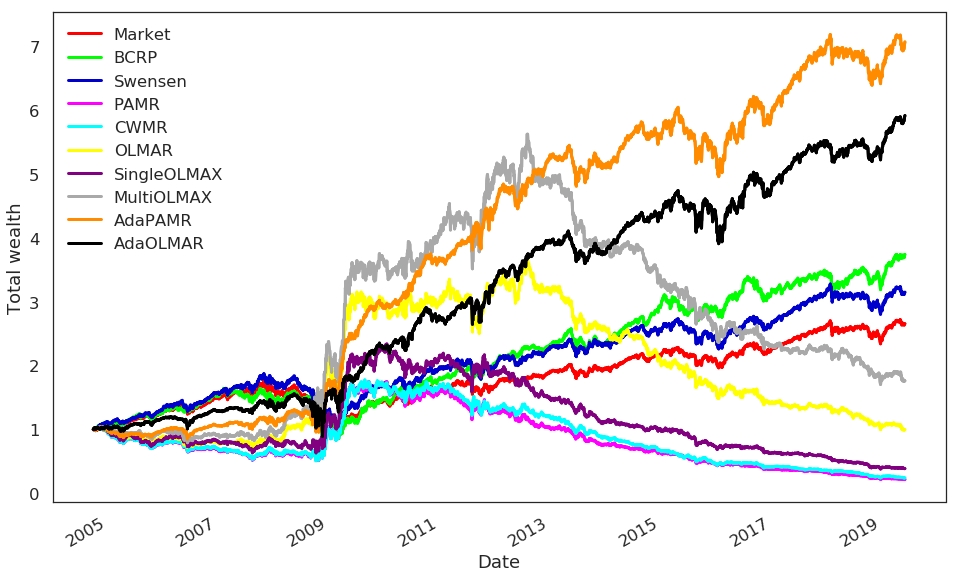
\includegraphics[width=\textwidth, height=\textheight, keepaspectratio]{etf-cumwealth-with-fees-and-adaAlgos}
%\caption{Cumulative wealth net of 0.1\% fees achieved by various strategies during the entire trading periods associated with the ETF data set (see Table~\ref{tab:etf-dataset}).}
%\label{fig:etf-cumwealth-with-adaAlgos}
%\end{figure}
%
%Table~\ref{tab:olps-metrics-etfs} reports the performance metrics of all the aforementioned algorithms on the ETF data set, in addition to the remaining ones enumerated in Section~\ref{sec:comparison-approaches}. As one would expect from Figure~\ref{fig:etf-cumwealth-with-adaAlgos}, AdaPAMR and AdaOLMAR dominate in terms of annual percentage yield. Furthermore, AdaPAMR is the least risky from a drawdown perspective, and exhibits the highest Sharpe ratio, AdaOLMAR having the third highest. The table also reveals that online Newton step (ONS) is a very competitive strategy in this setting, being the second best in terms of maximum drawdown risk and Sharpe ratio.
%
%\begin{table}
%  \caption{Performance metrics achieved by various OLPS algorithms on the ETF data set from Table~\ref{tab:etf-dataset}, subject to transaction fees of 0.1\%. The top two results are highlighted in \textbf{bold}.}
%  \label{tab:olps-metrics-etfs}
%  \centering
%  \resizebox{\textwidth}{!}{\begin{tabular}{lcccc}
%      \toprule
%      Algorithm & APY (\%) & Volatility Risk (\%) & MDD Risk (\%) & Sharpe Ratio \\
%      \midrule
%Market	& 6.87 & 14.90 & 45.33 & 0.45 \\
%Best stock & 8.83 & 18.47 & 55.45 & 0.46 \\
%BCRP & 9.39	& 18.81 & 47.97 & 0.48 \\
%Swensen	& 8.12 & 17.33 & 47.31 & 0.45 \\
%\\
%UP & 7.74 & \textbf{14.61} & 42.04 & 0.51 \\
%EG & 7.83 & \textbf{14.61} & 41.72 & 0.52 \\
%ONS & 10.14 & 15.22 & \textbf{32.64} & \textbf{0.63} \\
%\\
%PAMR & -9.95 & 24.54 & 87.74 & -0.43 \\
%CWMR & -9.29 & 24.75 & 86.54 & -0.39 \\
%OLMAR & -0.04 & 24.87 & 73.10 & -0.00 \\
%\\
%SingleOLMAX	& -6.29 & 24.61 & 83.81 & -0.26 \\
%MultiOLMAX-S & 3.93	& 24.62 & 69.71 & 0.16 \\
%MultiOLMAX-E & 5.84	& 24.84 & 66.34 & 0.23 \\
%\\
%AdaPAMR	& \textbf{14.24} & 18.87 & \textbf{26.79} & \textbf{0.71} \\
%AdaOLMAR & \textbf{12.86} & 21.13 & 42.81 & 0.57 \\
%      \bottomrule
%  \end{tabular}}
%\end{table}
%
%We end this chapter by recommending AdaPAMR as a general-purpose online portfolio selection algorithm that offers transaction-cost robustness and versatility to handle different asset classes and market regimes thanks to its hyperparameter-free nature.


\subsection{Empirical evaluation}
\label{sec:adapamr-eval}

\begin{mccorrection}
We now turn to implement the AdaPAMR and AdaOLMAR algorithms on the ETFs mentioned in Table~\ref{tab:etf-dataset}. Figure~\ref{fig:etf-cumwealth-with-adaAlgos} illustrates their respective cumulative wealth net of a transaction fee of 0.1\%, along with those achieved by the three benchmarks (Market, BCRP and the Swensen portfolio) and the non-adaptive reversion strategies (CWMR, PAMR, OLMAR, SingleOLMAX and MultiOLMAX). Furthermore, in order to empirically motivate the benefits of our approach, we include analogous variants of AdaPAMR and AdaOLMAR in which the learning rate is fixed to a schedule of $1/\sqrt{t}$, as in \citep{zinkevich03}. Perhaps at the expense of an abuse of terminology, we named these `AdaPAMR with $1/\sqrt{t}$ annealing' and `AdaOLMAR  with $1/\sqrt{t}$ annealing', respectively.

In comparison to the benchmarks, both the AdaPAMR and AdaOLMAR methods would have realised big gains at the end of the subprime mortgage crisis and, unlike their non-adaptive counterparts, managed to maintain that positive momentum all along thereafter, especially AdaPAMR. This explains the large discrepancy between their respective terminal wealths and that of all the other strategies plotted in the chart. Additionally, we notice that the variants of AdaPAMR and AdaOLMAR with Zinkevich's learning-rate schedule of $1/\sqrt{t}$ barely beat the Swensen portfolio, making them unattractive choices.
\end{mccorrection}
\begin{figure}[H]
\centering
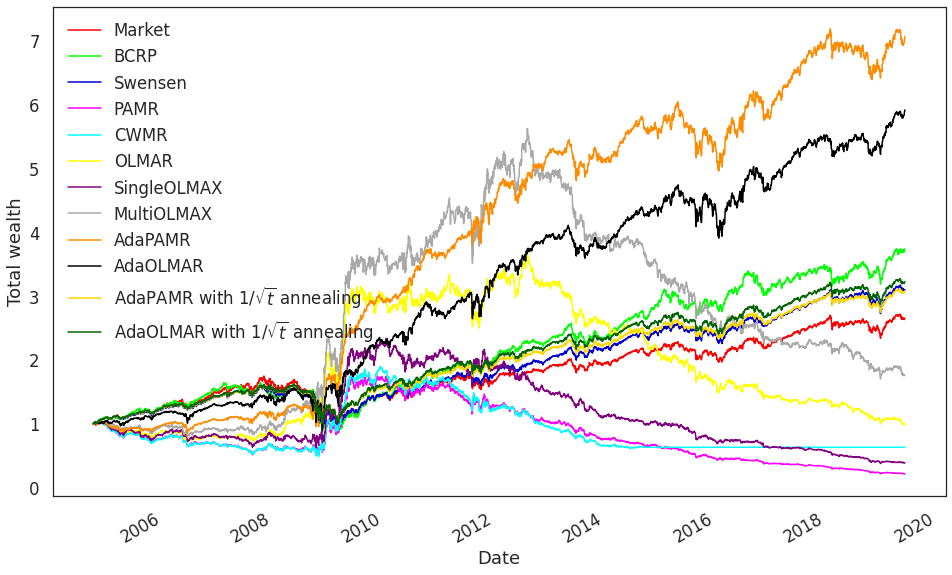
\includegraphics[width=\textwidth, height=\textheight, keepaspectratio]{etf-cumwealth-with-fees-and-adaAlgos-NEW}
\caption{Cumulative wealth net of 0.1\% fees achieved by various strategies during the entire trading periods associated with the ETF data set (see Table~\ref{tab:etf-dataset}).}
\label{fig:etf-cumwealth-with-adaAlgos}
\end{figure}

\begin{mccorrection}
Table~\ref{tab:olps-metrics-etfs} reports the performance metrics of all the aforementioned algorithms on the ETF data set, in addition to the remaining ones enumerated in Section~\ref{sec:comparison-approaches}. As one would expect from Figure~\ref{fig:etf-cumwealth-with-adaAlgos}, AdaPAMR and AdaOLMAR dominate in terms of annual percentage yield. Furthermore, AdaPAMR is the least risky from a drawdown perspective, and exhibits the highest Sharpe ratio.
\end{mccorrection}
\begin{table}
  \caption{Performance metrics achieved by various OLPS algorithms on the ETF data set from Table~\ref{tab:etf-dataset}, subject to transaction fees of 0.1\%. The top two results are highlighted in \textbf{bold}.}
  \label{tab:olps-metrics-etfs}
  \centering
  \resizebox{\textwidth}{!}{\begin{tabular}{lcccc}
      \toprule
      Algorithm & APY (\%) & Volatility Risk (\%) & MDD Risk (\%) & Sharpe Ratio \\
      \midrule
Market	& 6.87 & 14.90 & 45.33 & 0.45 \\
Best stock & 8.83 & 18.47 & 55.45 & 0.46 \\
BCRP & 9.39	& 18.81 & 47.97 & 0.48 \\
Swensen	& 8.12 & 17.33 & 47.31 & 0.45 \\
\\
UP & 7.74 & 14.61 & 42.04 & 0.51 \\
EG & 7.83 & 14.61 & 41.72 & 0.52 \\
ONS & 10.14 & 15.22 & \textbf{32.64} & 0.63 \\
\\
PAMR & -9.95 & 24.54 & 87.74 & -0.43 \\
CWMR & -9.29 & 24.75 & 86.54 & -0.39 \\
OLMAR & -0.04 & 24.87 & 73.10 & -0.00 \\
\\
SingleOLMAX	& -6.29 & 24.61 & 83.81 & -0.26 \\
MultiOLMAX-S & 3.93	& 24.62 & 69.71 & 0.16 \\
MultiOLMAX-E & 5.84	& 24.84 & 66.34 & 0.23 \\
\\
AdaPAMR with $1/\sqrt{t}$ annealing	& 8.50 & \textbf{12.95} & 37.07 & \textbf{0.66} \\
AdaOLMAR with $1/\sqrt{t}$ annealing	& 8.93 &	 \textbf{13.79} & 38.16 & 0.65 \\
AdaPAMR	& \textbf{14.24} & 18.87 & \textbf{26.79} & \textbf{0.71} \\
AdaOLMAR & \textbf{12.86} & 21.13 & 42.81 & 0.57 \\
      \bottomrule
  \end{tabular}}
\end{table}

We end this chapter by recommending AdaPAMR as a general-purpose online portfolio selection algorithm that offers transaction-cost robustness and versatility to handle different asset classes and market regimes thanks to its hyperparameter-free nature.

\part{Conclusions and Extensions}
\chapter{Summary Conclusions}
\label{ch:summary-conclusions}

\minitoc

This thesis has contributed novel modelling techniques for sequential data, with a focus on online portfolio selection. The contributions, set out in the three chapters comprising Part II, are unified under the title `Bayesian Online Learning for Portfolio Management', and split into three approximately-homogeneous contribution chapters. Chapter~\ref{ch:pa-extensions} discussed generalisations of and probabilistic inference in a particular class of online model known as `online passive-aggressive learning', in which a weight vector is passively maintained or aggressively updated from round to round depending on whether or not it correctly predicted the most recent example. Chapter~\ref{ch:oo} dealt with the topic of online convex optimisation in dynamic environments, and by incorporating insight from Chapter~\ref{ch:pa-extensions}, contributed two novel online and data-dependent adaptation methods for tuning the learning rate in online gradient descent, arguably the most popular algorithm in this context. Finally, in Chapter~\ref{ch:empirical-eval}, we demonstrated the superiority of our proposed methods over existing ones in online portfolio selection experiments involving real-world data from the equity, fixed income and real-estate markets.

This chapter seeks to conclude the thesis by drawing together summary results and conclusions of the contributions set out in Part II.


\section{Extending Passive-Aggressive Learning}

Chapter~\ref{ch:pa-extensions} formulated some generalisations and a Bayesian treatment of online passive-aggressive (PA) algorithms, which have been used in various fields including finance \citep{pamr, olmar}, recommendation systems \citep{blondel14} and natural language processing \citep{bayespa}. The generic PA update rule (as per Chapter~\ref{ch:ol}, Eq. \eqref{eq:generic-pa-update-rule}) is intuitive, straightforward to implement and universally applicable to online classification, regression and uniclass tasks. However, it suffers from some drawbacks, namely \textit{i}) it is only valid for the $\epsilon$-insensitive loss function, \textit{ii}) it does not provide any guidelines as to how to set the underlying hyperparameters, and \textit{iii}) it is a point estimate, thereby failing to capture model and prediction uncertainty.

To address the first of these issues, we derived a generalised passive-aggressive learning framework, by replacing the $\epsilon$-insensitive loss in the generic PA learning problem's constraint (i.e.\ the constraint in Eq. \eqref{eq:generic-pa-optpb}) with a general loss function. By approximating this general loss function with its first-order Taylor polynomial around the current weight vector, we are able to apply the same solution methods used to arrive at the PA weight updates. The algorithms so defined overcome the specialisation of the original PA framework to the $\epsilon$-insensitive loss while maintaining elegance and scalability. Moreover, the derivation is didactically useful in the sense that it provides inspiration and insight for other algorithms described later in the thesis, including the passive-aggressive convex optimisation algorithm~\ref{alg:paco}.

A Bayesian treatment of PA learning was also discussed, motivated by a desire to circumvent the remaining aforementioned shortcomings, i.e.\ points \textit{ii}) and \textit{iii}), in addition to the framework's inability to take into account how the data are distributed. Inspired by the pseudo-likelihood and data-augmentation ideas from \citep{polson&scott}, the mixture representation \eqref{eq:ilf-likelihood-mixture-rep} is the key ingredient, since it significantly reduces the complexity of inference by bringing Bayesian tools for Gaussian linear models to bear on PA algorithms. We then contributed a novel online scheme for variational posterior inference in an augmented variable space, that additionally offers the benefit of automatic hyperparameter tuning. To make robust predictions, the approximate posterior of model weights, rather than point estimates as in traditional PA methods, is used. Once the approximate posterior is obtained from a given data set, we can regard it as the model prior when dealing with the arrival of new data, which makes the model suitable for online scenarios. 


\section{Adaptive Gradient Methods for Dynamic Online Optimisation}

Online convex optimisation is a prevalent topic in machine learning and its application in dynamic environments has recently received considerable interest in the literature. Whilst the online gradient descent algorithm is appealing in this context due to its numerous advantages, adjusting its learning-rate parameter is an important unresolved problem which requires tuning in practice. Previous work has relied on theoretical learning-rate schedules, under the assumption that certain parameters of the loss function such as smoothness or strong convexity constants are known. However, in practice, such parameters are unknown and the burden of specification rests upon the practitioner.

We presented a novel method for dynamically updating the learning-rate parameter according to the gradients received so far, which we believe provides a significant contribution to the long-standing problem of tuning this parameter. Unlike the schemes previously used in the literature, ours is completely hyperparameter-free and can thus be readily deployed without any manual intervention. Moreover, its applicability extends beyond the field of online convex optimisation, in particular to neural-network training (see Section~\ref{sec:oo-further-work}).

The aforementioned method was derived in three steps. First, we determined in Section~\ref{sec:ogd-criterion} which optimisation problem online gradient descent implicitly solves. Second, we provided a maximum a posteriori interpretation thereof in Section~\ref{sec:probabilistic-ogd}, which revealed that the algorithm implicitly imposes an isotropic Gaussian prior over the weights whose precision parameter coincides with the inverse learning rate. Third, in Section~\ref{sec:learning-rate-inference}, we proceeded to integrate out this precision parameter so as to obtain the true weight posterior (i.e.\ the posterior conditioned on the data but not on the learning rate), whose optimisation yields hyperparameter-free online gradient descent updates.

Finally, we also discussed how to adapt the generalised passive-aggressive learning framework from Section~\ref{sec:gpa} to the dynamic bandit setting. While we were able to readily carry out this adaptation, it still required estimating the latent gradients as a preliminary step, which we covered in Section~\ref{sec:gradient-estimates}.

Taken together, the two approaches summarised above represent a significant contribution to the literature on online convex optimisation in dynamic environments.


\section{Application to Online Portfolio Selection}

This chapter culminates our research on online Bayesian techniques for portfolio management. It presents two novel families of algorithms for online portfolio selection, namely `online maximum reversion' and `adaptive online mean reversion', in Sections~\ref{sec:olmax} and~\ref{sec:ada-mr}, respectively. The proposed approaches are able to overcome the limitations of existing state-of-the-art online portfolio selection strategies, discussed in Section~\ref{sec:empirical-eval-intro}, and were shown to deliver superior performance on the equity data sets widely used in literature and a real-world cross-asset data set, respectively.

Online maximum reversion is built upon the assumption that price-relative vectors change slowly over time. This was corroborated for the stock-market data set in Section~\ref{sec:olmax-motivation}, and permits the use of the loss function at time $t$ (parameterised by the $t$th price-relative vector) as a surrogate for the unobserved loss at time $t+1$. With this in mind, we approximate the optimal portfolio $\mathbf{b}_{t+1}^*$ by the minimiser $\mathbf{b}_{t+1}$ of the current loss function, as detailed in Eq. \eqref{eq:single-olmax-criterion}. This leads to a hyperparameter-free single-period online reversion algorithm that does not suffer from data-snooping bias, unlike any of its competitors. We also explored a multiperiod variant to alleviate the data-snooping issue affecting the most powerful online mean-reversion strategy known to date, namely `online moving average reversion'.

In addition to the data-snooping bias, existing online portfolio selection techniques are fraught with selection bias as they are restricted to equity markets and, to fix this limitation, we devised adaptive online mean reversion strategies. To this end, we started from the passive-aggressive mean reversion and online moving average reversion algorithms, and expressed their respective portfolio updates in the form of online gradient descent updates with data-driven, but hyperparameter-dependent, learning-rate schedules (see Eq. \eqref{eq:pamr-portfolio} and \eqref{eq:olmar-portfolio}, respectively). To reduce this hyperparameter dependency, we then replaced these learning-rate schedules with their equivalent maximum posterior counterparts derived from Eq. \eqref{eq:mapgrad-learning-rate}. The resulting strategies are more amenable to asset classes beyond equities, as well as to reasonable transaction fees.
\chapter{Further Work}
\label{ch:further-work}

\minitoc

It is interesting to consider how one may further extend the studies presented throughout the thesis, and this chapter seeks to lay the foundations for many future avenues of research.


\section{Extending Passive-Aggressive Learning}

Whilst the generalised passive-aggressive (GPA) framework of Chapter~\ref{ch:pa-extensions} is flexible by construction of the model and algorithms, there are some simple ways in which it can be enhanced. First of all, it is possible to augment the model by substituting the Mahalanobis for the Euclidean distance in the objective of Eq. \eqref{eq:gpa-optpb}, so as to explicitly account for the distribution of the data. A further extension of the model is possible by noting that it is formulated in terms of a deterministic point-estimation problem governed by a set of user-defined hyperparameters: the approach fails to capture model/prediction uncertainty and induces dependence on hyperparameter settings.

\subsection{Bayesian Generalised Passive-Aggressive Learning}

We propose a unified Bayesian approach that encompasses the suggested enhancements. Our starting point is the soft GPA criterion in Eq. \eqref{eq:gpa-optpb-I}, but without the loss expansion in the constraint and with the Mahalanobis instead of the Euclidean distance in the objective. By analogy with Eq. \eqref{eq:PA-I-optpb-altform}, this modified criterion can be rewritten as
\begin{equation}
\label{eq:modified-gpa-I-optpb}
	\min_{\mathbf{w} \in \mathbb{R}^n} \;
	\Big\{C\ell_{t}(\mathbf{w}) + \frac{1}{2}(\mathbf{w} - \mathbf{w}_t)^\text{T}\boldsymbol{\Sigma}_{t}^{-1}(\mathbf{w} - \mathbf{w}_t)\Big\},
\end{equation}
where $\boldsymbol{\Sigma}_{t}$ denotes the covariance matrix of the weight vector at round $t$.

Solving \eqref{eq:modified-gpa-I-optpb} is equivalent to finding the mode of the pseudo-posterior distribution $p(\mathbf{w}|\mathcal{D}_t, \boldsymbol{\theta}_t, C)$ defined by
\begin{equation}
\begin{split}
	p(\mathbf{w}|\mathcal{D}_t, \boldsymbol{\theta}_t, C) 
	&\propto \exp\Big\{-C\ell_{t}(\mathbf{w}) - \frac{1}{2}(\mathbf{w} - \mathbf{w}_t)^\text{T}\boldsymbol{\Sigma}_{t}^{-1}(\mathbf{w} - \mathbf{w}_t)\Big\}
	\\	
	&\propto L_t(\mathbf{w}|C)p(\mathbf{w}|\boldsymbol{\theta}_t),
\end{split}
\end{equation}
where $\mathcal{D}_t$ is the datum implicit in $\ell_t(\cdot)$, and $\boldsymbol{\theta}_t \equiv \{\mathbf{w}_t, \boldsymbol{\Sigma}_{t}\}$. The data-dependent factor is a pseudo-likelihood contribution given by
\begin{equation}
	L_t(\mathbf{w}|C) = \exp\Big\{-C\ell_{t}(\mathbf{w})\Big\},
\end{equation}
where the prefix `pseudo' refers to the fact that this quantity is un-normalised with respect to the observation $\mathcal{D}_t$, which also justifies our use of the name `pseudo-posterior'\footnote{In principle, one could work with an actual likelihood contribution if $L_t$ was replaced by its normalised value $\widetilde{L}_t$, but we work with $L_t$ instead because it leads to the traditional GPA weight estimates. This is common practice in the Bayesian treatment of other frequentist supervised-learning methods (see, e.g., \citep{polson&scott, deng16}).}.
The second factor, which we recognise as a Gaussian of the form
\begin{equation}
	p(\mathbf{w}|\boldsymbol{\theta}_t)
	= \mathcal{N}(\mathbf{w}|\mathbf{w}_t,\, \boldsymbol{\Sigma}_{t}),
\end{equation}
acts as an \emph{approximate posterior} replacing the true, but generally intractable and offline, posterior $p(\mathbf{w}|\mathcal{D}_{1:t})$. The parameter vector $\boldsymbol{\theta}_t$ can be thought of as a `summary statistic' for past observations, and needs to be updated at each step to incorporate new information.
%This paradigm was originally proposed in \citep[Section~6]{opper98}, and we also adopted it in Sections. 

\subsubsection{Variational inference}

In all but limited special cases, the function $L_t$ is not a simple squared exponential, resulting in a new pseudo-posterior $p(\mathbf{w}|\mathcal{D}_t, \boldsymbol{\theta}_t, C)$ of a non-standard form. Inevitably, therefore, approximations are required. When the dimension $n$ of the weight vector $\mathbf{w}$ is large, finding an accurate approximation is, in general, non-trivial. Our particular interest here is to form an approximation $p(\mathbf{w}|\boldsymbol{\theta}_{t+1})$ in which the parameters $\boldsymbol{\theta}_{t+1}$ are chosen so as to ensure that $p(\mathbf{w}|\boldsymbol{\theta}_{t+1})$ is as similar as possible to $p(\mathbf{w}|\mathcal{D}_t, \boldsymbol{\theta}_t, C)$.

We consider a Kullback-Leibler (KL) approach based on fitting a Gaussian to $p(\mathbf{w}|\boldsymbol{\theta}_{t+1})$, which is the most natural choice since $p(\mathbf{w}|\boldsymbol{\theta}_t)$ is also Gaussian and $p(\mathbf{w}|\boldsymbol{\theta}_{t+1})$ serves as the prior for $p(\mathbf{w}|\mathcal{D}_{t+1}, \boldsymbol{\theta}_{t+1}, C)$. Defining
\begin{equation}
	\widetilde{p}(\mathbf{w}|\mathcal{D}_t, \boldsymbol{\theta}_t, C)
	= \frac{L_t(\mathbf{w}|C)\mathcal{N}(\mathbf{w}|\mathbf{w}_t,\, \boldsymbol{\Sigma}_{t})}{Z},
	\qquad Z = \int L_t(\mathbf{w}|C)\mathcal{N}(\mathbf{w}|\mathbf{w}_t,\, \boldsymbol{\Sigma}_{t}) \, \mathrm{d}\mathbf{w},
\end{equation}
and fitting a Gaussian $p(\mathbf{w}|\boldsymbol{\theta}_{t+1}) = \mathcal{N}(\mathbf{w}|\mathbf{w}_{t+1},\, \boldsymbol{\Sigma}_{t+1})$ based on minimising the KL divergence $\mathrm{KL}[p(\mathbf{w}|\boldsymbol{\theta}_{t+1}) \, || \, \widetilde{p}(\mathbf{w}|\mathcal{D}_t, \boldsymbol{\theta}_t, C)]$, we obtain the bound $\log Z \geq \mathcal{B}_{t}(\boldsymbol{\theta}_{t+1})$ with
\begin{equation}
\begin{split}
	\mathcal{B}_{t}(\boldsymbol{\theta}_{t+1})
	& \equiv -\langle\log p(\mathbf{w}|\boldsymbol{\theta}_{t+1})\rangle - \frac{1}{2}\log|2\pi\boldsymbol{\Sigma}_{t}|
	\\
	& \quad -\frac{1}{2}\langle(\mathbf{w} - \mathbf{w}_t)^\text{T}\boldsymbol{\Sigma}_{t}^{-1}(\mathbf{w} - \mathbf{w}_t)\rangle + \langle\log L_t(\mathbf{w}|C)\rangle,
\end{split}
\end{equation}
where $\langle\cdot\rangle$ denotes the expectation with respect to $p(\mathbf{w}|\boldsymbol{\theta}_{t+1})$. One then numerically finds the best parameters $\boldsymbol{\theta}_{t+1}$ that maximise the bound.

Since the entropy of a Gaussian is trivial, the only potentially problematic term in evaluating $\mathcal{B}_{t}$ is $\langle\log L_t(\mathbf{w}|C)\rangle$. An important class of functions for which $\langle\log L_t(\mathbf{w}|C)\rangle_{\mathcal{N}(\mathbf{w}|\mathbf{w}_{t+1},\, \boldsymbol{\Sigma}_{t+1})}$ is computationally tractable is when $L_t(\mathbf{w}|C) = L(\mathbf{w}^\text{T}\mathbf{x}_t|C)$ for some fixed vector $\mathbf{x}_t$\footnote{This is the case for linear hypotheses, in which $\mathbf{x}_t$ represents the input vector at time $t$, so that the loss function takes the form $\ell_{t}(\mathbf{w}) = \ell(\mathbf{w}^\text{T}\mathbf{x}_t)$.}. In this case, the projection $\mathbf{w}^\text{T}\mathbf{x}_t$ is also Gaussian distributed and we have
\begin{equation}
	\langle\log L(\mathbf{w}^\text{T}\mathbf{x}_t|C)\rangle_{\mathcal{N}(\mathbf{w}|\mathbf{w}_{t+1},\, \boldsymbol{\Sigma}_{t+1})}
	= \langle\log L(y_{t+1}|C)\rangle_{\mathcal{N}(y_{t+1}|\mathbf{w}_{t+1}^\text{T}\mathbf{x}_t,\, \mathbf{x}_t^\text{T}\boldsymbol{\Sigma}_{t+1}\mathbf{x}_t)},
\end{equation}
which can be readily computed using any one-dimensional integration routine. Explicitly, as a function of $\boldsymbol{\theta}_{t+1}$, we have
\begin{equation}
\begin{split}
	2\mathcal{B}_{t}(\boldsymbol{\theta}_{t+1})
	&= -\log|\boldsymbol{\Sigma}_{t+1}| + n + \log|\boldsymbol{\Sigma}_{t}| - \mathrm{Tr}[\boldsymbol{\Sigma}_{t}^{-1}(\boldsymbol{\Sigma}_{t+1} + (\mathbf{w}_{t+1} - \mathbf{w}_{t})(\mathbf{w}_{t+1} - \mathbf{w}_{t})^\text{T})]
	\\	
	&\qquad + 2\langle\log L(y_{t+1}|C)\rangle_{\mathcal{N}(y_{t+1}|\mathbf{w}_{t+1}^\text{T}\mathbf{x}_t,\, \mathbf{x}_t^\text{T}\boldsymbol{\Sigma}_{t+1}\mathbf{x}_t)}.
\end{split}
\end{equation}
Whilst, in general, the variational bounds are non-concave in their variational parameters, provided $L$ is log-concave, then $\mathcal{B}_{t}(\mathbf{w}_{t+1}, \, \boldsymbol{\Sigma}_{t+1})$ is jointly concave in $\mathbf{w}_{t+1}$ and $\boldsymbol{\Sigma}_{t+1}$. By using structured covariance matrices $\boldsymbol{\Sigma}_{t+1}$, the method is scalable to very high dimensional problems \citep{challis11}.

\subsection{Online Bayesian Passive-Aggressive Classification}

The case of online passive-aggressive classification, which is characterised by the hinge	-loss function $\ell_t(\mathbf{w}) = \max\{0, 1 - y_t(\mathbf{w}\cdot\mathbf{x}_t)\}$, is to be treated differently. This is because, as shown in \citep[Theorem~1]{polson&scott}, the pseudo-likelihood corresponding to the hinge loss can be represented as a location-scale mixture of Gaussians, by introducing latent variables $\lambda_t$ such that
\begin{equation}
	L_{t}(\mathbf{w}|\gamma)
	= \exp\Big\{-2\gamma\max\big\{0, 1 - y_t(\mathbf{w}\cdot\mathbf{x}_t)\big\}\Big\}
	= \int_{0}^{\infty} L_{t}(\mathbf{w}, \lambda_t|\gamma)\,\mathrm{d}\lambda_t,
\end{equation}
where
\begin{equation}
	L_{t}(\mathbf{w}, \lambda_t|\gamma)
	= \frac{\sqrt{\gamma}}{\sqrt{2\pi\lambda_t}}\exp\Big\{-\frac{[1+\lambda_t-y_t(\mathbf{w}\cdot\mathbf{x}_t)]^2}{2\gamma^{-1}\lambda_t}\Big\}.
\end{equation}
This result allows us to pair observation $y_t$ with a latent variable $\lambda_t$ in such a way that $L_t$ is the \emph{marginal} counterpart of a joint pseudo-likelihood function $L_{t}(\mathbf{w}, \lambda_t|\gamma)$ in which $\mathbf{w}$ appears as part of a quadratic form. This implies that $ L_{t}(\mathbf{w}, \lambda_t|\gamma)$ is conjugate to a multivariate normal prior distribution, which in turn allows the optimality criterion of online PA classifcation to be expressed as a conditionally Gaussian linear model, for which approximate Bayesian inference is trivial. We refer the interested reader to \citep{polson&scott} and Section~\ref{sec:Bayes-PA} for further details on different inference schemes.

\subsection{An Alternative Approach to Bayesian GPA Learning}

The theory of normal variance-mean mixtures, alluded to in the previous paragraph, is highly flexible as it enables the derivation of a data-augmentation scheme for a class of common regularization problems. \citet{polson&scott13} demonstrate this method on several examples, including sparse quantile regression and binary logistic regression. Their work can be borrowed and adapted to develop a data-augmentation approach to Bayesian generalised passive-aggressive learning.
 



\section{Adaptive Gradient Methods for Dynamic Online Optimisation}
\label{sec:oo-further-work}

%As we already mentioned in Section~\ref{sec:related-work}, the authors of \citep{badam} give a probabilistic interpretation of adaptive subgradient optimisation methods (in particular, ADAM \citep{adam}) so as to make probabilistic inferences regarding the weights of neural networks, and in particular, to obtain cheap uncertainty estimates thereof. Although their focus is not on developing a self-tuning scheme for the learning rate parameter, their main theoretical result, exposed in Eq. (14), can be additionally harnessed for this purpose, and it would be both of theoretical and practical importance to explore this avenue, borrowing results from Chapter~\ref{ch:oo}.
\begin{mccorrection}
As we already mentioned in Section~\ref{sec:related-work}, the authors of \citep{badam} give a probabilistic interpretation of adaptive optimisation algorithms (in particular, ADAM \citep{adam}) so as to make probabilistic inferences regarding the weights of neural networks, and in particular, to obtain cheap uncertainty estimates thereof. Although their focus is not on developing a self-tuning scheme for the learning rate parameter, their main theoretical result, exposed in Eq. (14), can be additionally harnessed for this purpose, and it would be both of theoretical and practical importance to explore this avenue, borrowing results from Chapter~\ref{ch:oo}.
\end{mccorrection}


\section{Application to Online Portfolio Selection}

Our online portfolio selection experiments could be enriched with some simple extensions. Firstly, we have thus far only considered trading stocks/ETFs on a daily basis. We may wish to tackle other asset classes and/or rebalancing frequencies (potentially intra-day) that also exhibit mean-reverting patterns. For example, there is overwhelming statistical evidence on the mean reversion of interest rates, which can be monetised by trading fixed-income instruments.

Long-short portfolios would form another interesting extension of our online portfolio selection framework, which is confined to long-only portfolios. Unlike the asset management industry, this type of portfolio is popular among hedge funds whose bread and butter is \emph{statistical arbitrage} (e.g., long-short equity), and so this avenue would be of extreme practical importance to such financial market participants.


%% APPENDICES %% 
% Starts lettered appendices, adds a heading in table of contents, and adds a
%    page that just says "Appendices" to signal the end of your main text.
\startappendices
% Add or remove any appendices you'd like here:
\chapter{Mathematical Background}

\minitoc




\section{Probability and Information Theory}


\subsection{Joint, marginal and conditional probability}

Let the $n$ (discrete or continuous) random variables $y_1, \ldots, y_n$ have a joint joint probability probability $p(y_1, \ldots, y_n)$, or $p(\mathbf{y})$ for short\footnote{One can deal with more general cases where the density function does not exist by using the distribution function.}. Technically, one ought to distinguish between probabilities (for discrete variables) and probability densities for continuous variables. Throughout the thesis we commonly use the term `probability' to refer to both. Let us partition the variables in $\mathbf{y}$ into two groups, $\mathbf{y}_A$ and $\mathbf{y}_B$, where $A$ and $B$ are two disjoint sets whose union is the set $\{1, \ldots, n\}$, so that $p(\mathbf{y}) = p(\mathbf{y}_A, \mathbf{y}_B)$. Each group may contain one or more variables.

The \emph{marginal} probability of $\mathbf{y}_A$ is given by
\begin{equation}
	p(\mathbf{y}_A) = \int  p(\mathbf{y}_A, \mathbf{y}_B) \, \mathrm{d}\mathbf{y}_B.
\end{equation}
The integral is replaced by a sum if the variables are discrete valued. Notice that if the set $A$ contains more than one variable, then the marginal probability is itself a joint probability---whether it is referred to as one or the other depends on the context. If the joint distribution is equal to the product of the marginals, then the variables are said to be \emph{independent}, otherwise they are \emph{dependent}.

The \emph{conditional} probability function is defined as
\begin{equation}
	p(\mathbf{y}_A|\mathbf{y}_B) = \frac{p(\mathbf{y}_A, \mathbf{y}_B)}{p(\mathbf{y}_B)},
\end{equation}
defined for $p(\mathbf{y}_B) > 0$, as it is not meaningful to condition on an impossible event. If $\mathbf{y}_A$ and $\mathbf{y}_B$ are independent, then the marginal $p(\mathbf{y}_A)$ and the conditional $p(\mathbf{y}_A|\mathbf{y}_B)$ are equal.

Using the definitions of both $p(\mathbf{y}_A|\mathbf{y}_B)$ and $p(\mathbf{y}_B|\mathbf{y}_A)$ we obtain \emph{Bayes' theorem}:
\begin{equation}
\label{eq:bayes-thm}
	p(\mathbf{y}_A|\mathbf{y}_B) = \frac{p(\mathbf{y}_B|\mathbf{y}_A)p(\mathbf{y}_A)}{p(\mathbf{y}_B)}.
\end{equation}
Since conditional distributions are themselves probabilities, one can use all of the above also when further conditioning on other variables. For example, in supervised learning, one often conditions on the inputs throughout, which would lead e.g.\ to a version of Bayes' rule with additional conditioning on $X$ in all four probabilities in Eq.~\eqref{eq:bayes-thm}.


\subsection{Change of variables}

For a univariate continuous random variable $x$ with distribution $p(x)$, the transformation $y = f(x)$, where $f(x)$ is a monotonic function, has distribution
\begin{equation}
\label{eq:pdf-chg-of-vars}
	p(y) = p(x)\left|\frac{df}{dx}\right|^{-1},
	\qquad x = f^{-1}(y).
\end{equation}
For multivariate $\mathbf{x}$ and bijection $\mathbf{f}(\mathbf{x})$, then $\mathbf{y} = \mathbf{f}(\mathbf{x})$ has distribution
\begin{equation}
\label{eq:pdf-chg-of-vars-multi}
	p(\mathbf{y}) = p(\mathbf{x} = \mathbf{f}^{-1}(\mathbf{y}))\left|\mathrm{det}\left(\frac{\partial \mathbf{f}}{\partial \mathbf{x}}\right)\right|^{-1},
\end{equation}
where the Jacobian matrix has elements
\begin{equation}
	\left[\frac{\partial \mathbf{f}}{\partial \mathbf{x}}\right]_{i,\, j}
	= \frac{\partial f_{i}(\mathbf{x})}{\partial x_j}.
\end{equation}
Sometimes, one needs to consider transformations between different dimensions. For example, if $\mathbf{z}$ has lower dimension than $\mathbf{x}$, then one may introduce additional variables $\mathbf{z}^\prime$ to define a new multivariate $\mathbf{y} = (\mathbf{z},\, \mathbf{z}^\prime)$ with the same dimension as $\mathbf{x}$. Then one applies the transformation \eqref{eq:pdf-chg-of-vars-multi} to give the distribution on the joint variables $\mathbf{y}$, from which $p(\mathbf{z})$ can be obtained by marginalisation.


\subsection{Entropy and Kullback-Leibler divergence}
\label{sec:entropy}

The \emph{entropy} $\mathrm{H}[p(\mathbf{x})]$ of a distribution $p(\mathbf{x})$ is a non-negative measure of the amount of `uncertainty' in the distribution, and is defined as
\begin{equation}
	\mathrm{H}[p(\mathbf{x})] \equiv -\int p(\mathbf{x})\log p(\mathbf{x}) \, \mathrm{d}\mathbf{x}.
\end{equation}
The integral is substituted by a sum for discrete variables. Entropy is measured in \emph{bits} if the log is to the base 2 and in \emph{nats} in the case of the natural log.

The Kullback-Leibler (KL) divergence (or relative entropy) $\mathrm{KL}(p \Vert q)$ between two distributions $p(\mathbf{x})$ and $q(\mathbf{x})$ is defined as
\begin{equation}
	\mathrm{KL}(p \Vert q) = \int p(\mathbf{x})\log\frac{p(\mathbf{x})}{q(\mathbf{x})} \, \mathrm{d}\mathbf{x}.
\end{equation}
It is easy to show that $\mathrm{KL}(p \Vert q) \geq 0$, with equality if $p = q$ (almost everywhere). The KL divergence can be viewed as the extra number of nats needed on average to code data generated from a source $p(\mathbf{x})$ under the distribution $q(\mathbf{x})$ as opposed to $p(\mathbf{x})$.




\section{Convex Optimisation}

In this section, we give a gentle introduction to convex optimisation and present some basic algorithms for solving convex mathematical programs. A broad and significantly more detailed literature exists, and the reader is referred to \cite{nemirovski, rockafellar, fletcher, bv_cvxbook, borwein, bubeck}, among others. We give here only the most elementary analysis, and focus on the techniques that are of use to us throughout the thesis.

\subsection{Basic definitions and setup}
\label{sec:cvxopt-defs}

The goal in this chapter is to minimise a continuous and convex function over a convex subset of the Euclidean space. Henceforth, let $\mathcal{K} \subseteq \mathbb{R}^d$ be a bounded, convex and compact set in the Euclidean space. 
\begin{mydef}
\label{def:diameter}
The \emph{diameter} of $\mathcal{K}$ is defined as
\begin{equation}
\mathrm{diam}(\mathcal{K}) \equiv \sup_{\mathbf{x}, \mathbf{y} \in \mathcal{K}} \, \Vert\mathbf{x} - \mathbf{y}\Vert_2,
\end{equation}
where $\Vert\mathbf{x}\Vert_2 = \sqrt{\mathbf{x}\cdot\mathbf{x}}$ is the Euclidean norm.
\end{mydef}
%We denote by $D$ an upper bound on the diameter of $\mathcal{K}$:
%\begin{equation}
%\forall \mathbf{x}, \mathbf{y} \in \mathcal{K},
%\Vert\mathbf{x} − \mathbf{y}\Vert_2 \leq D.
%\end{equation}
\begin{mydef}
\label{def:convex-set}
A set $\mathcal{K}$ is \emph{convex} if for any $\mathbf{x}, \mathbf{y} \in \mathcal{K}$, all the points on the line segment connecting $\mathbf{x}$ and $\mathbf{y}$ also belong to $\mathcal{K}$, i.e.\
\begin{equation}
\forall \alpha \in [0, 1], \quad \alpha\mathbf{x} + (1-\alpha)\mathbf{y} \in \mathcal{K}. 
\end{equation}
\end{mydef}
\begin{mydef}
\label{def:convex-function}
A function $f:\mathcal{K} \rightarrow \mathbb{R}$ is \emph{convex} if for any $\mathbf{x}, \mathbf{y} \in \mathcal{K}$,
\begin{equation}
\forall \alpha \in [0, 1], \quad f[(1-\alpha)\mathbf{x} + \alpha\mathbf{y}] \leq (1-\alpha)f(\mathbf{x}) + \alpha f(\mathbf{y}).
\end{equation}
Equivalently, if $f(\cdot)$ is differentiable, that is, its gradient $\nabla f(\mathbf{x})$ exists for all $\mathbf{x} \in \mathcal{K}$, then it is convex if and only if $\forall\mathbf{x}, \mathbf{y} \in \mathcal{K}$,
\begin{equation}
\label{eq:convex-function}
f(\mathbf{y}) \geq f(\mathbf{x}) + \nabla f(\mathbf{x}) \cdot(\mathbf{y} - \mathbf{x}).
\end{equation}
\end{mydef}
\begin{mydef}
\label{def:subgradient}
For convex and non-differentiable functions $f(\cdot)$, the \emph{subgradient} of $f(\cdot)$ at $\mathbf{x}$ is defined to be any vector $\mathbf{z}$ that satisfies the inequality
\begin{equation}
f(\mathbf{y}) \geq f(\mathbf{x}) + \mathbf{z}\cdot(\mathbf{y} - \mathbf{x}),
\end{equation}
for all $\mathbf{y} \in \mathcal{K}$. We call \emph{subdifferential set} the set of subgradients of $f(\cdot)$ at $\mathbf{x}$, and denote it as $\partial f(\mathbf{x})$. Furthermore, if $f(\cdot)$ is differentiable at $\mathbf{x}$, then $\partial f(\mathbf{x})$ contains a single element, namely the gradient $\nabla f(\mathbf{x})$ of $f(\cdot)$ at $\mathbf{x}$.
\end{mydef}

We denote by $G > 0$ an upper bound on the norm of the subgradients of $f(\cdot)$ over $\mathcal{K}$, i.e.\ $\Vert \nabla f(\mathbf{x})\Vert_2 \leq G$ for all $\mathbf{x} \in \mathcal{K}$. Such an upper bound implies that the function $f(\cdot)$ is Lipschitz continuous with parameter $G$.
\begin{mydef}
\label{def:lipschitz-continuity}
The function $f:\mathcal{K} \rightarrow \mathbb{R}$ is said to be \emph{Lipschitz continuous} with constant $G > 0$ if for all $\mathbf{x}, \mathbf{y} \in \mathcal{K}$, we have
\begin{equation}
|f(\mathbf{x}) - f(\mathbf{y})| \leq G\Vert\mathbf{x} - \mathbf{y}\Vert_2.
\end{equation}
\end{mydef}
The optimisation and machine learning communities study special types of convex functions that admit useful properties, which in turn allow for more efficient optimisation. Below, we define the most notable of these properties.
\begin{mydef}
\label{def:strongly-convex-function}
We say that a function $f : \mathcal{K} \rightarrow \mathbb{R}$ is $\lambda$-\emph{strongly convex} if
\begin{equation}
f(\mathbf{y}) \geq f(\mathbf{x}) + \nabla f(\mathbf{x})\cdot(\mathbf{y} - \mathbf{x}) + \frac{\lambda}{2}\Vert\mathbf{y} - \mathbf{x}\Vert_2^2,
\qquad \forall \, \mathbf{x}, \mathbf{y} \in \mathcal{K}.
\end{equation}
\end{mydef}
\begin{mydef}
\label{def:smooth-function}
A function $f : \mathcal{K} \rightarrow \mathbb{R}$ is $L$-\emph{smooth} if
\begin{equation}
f(\mathbf{y}) \leq f(\mathbf{x}) + \nabla f(\mathbf{x})\cdot(\mathbf{y} - \mathbf{x}) + \frac{L}{2}\Vert\mathbf{y} - \mathbf{x}\Vert_2^2,
\qquad \forall \, \mathbf{x}, \mathbf{y} \in \mathcal{K}.
\end{equation}
The latter condition is equivalent to the Lipschitz continuity of the gradients of $f(\cdot)$, with Lipschitz constant $L > 0$, i.e.\
\begin{equation}
\Vert\nabla f(\mathbf{x}) - \nabla f(\mathbf{y})\Vert_2 \leq L\Vert\mathbf{x} - \mathbf{y}\Vert_2,
\qquad \forall \, \mathbf{x}, \mathbf{y} \in \mathcal{K}.
\end{equation}
\end{mydef}
Throughout the thesis, we refer to $\lambda$-strongly convex functions simply as strongly convex functions. Similarly, we shall call smooth functions those functions satisfying Definition~\ref{def:smooth-function}.

If the function is twice-differentiable and admits a second derivative, known as the Hessian for a function of several variables, Definitions~\ref{def:strongly-convex-function} and~\ref{def:smooth-function} are equivalent to the following condition on the Hessian, which we denote by $\nabla^2 f(\mathbf{x})$:
\begin{equation}
\alpha\mathbf{I} \preceq \nabla^2 f(\mathbf{x}) \preceq \beta\mathbf{I},
\end{equation}
where $A \preceq B$ means the matrix $B - A$ is positive semi-definite.

When the function $f(\cdot)$ is both strongly convex and smooth, we say that it is $\gamma$-well-conditioned, where $\gamma$ is the ratio between strong convexity and smoothness, and is also known as the \emph{condition number} of $f(\cdot)$:
\begin{equation}
\gamma = \frac{\lambda}{L} \leq 1.
\end{equation}
\begin{example}
 The following functions are both strongly convex and smooth:
\begin{enumerate}
	\item A quadratic form $f(\mathbf{x}) = \mathbf{x}^\top A \mathbf{x} - 2\mathbf{b}^\top\mathbf{x}$, where $a\mathbf{I} \preceq A \preceq b\mathbf{I}$, for $a > 0$ and $b < \infty$;
	\item The regularised logistic loss $f(\mathbf{x}) = \log[1 + \exp(\mathbf{b}^\top\mathbf{x})] + \frac{\lambda}{2}\Vert\mathbf{x}\Vert_2^2$, where $\lambda > 0$.
\end{enumerate}
\end{example}

\subsection{Projections onto convex sets}
\label{sec:euclidean-projections}

Throughout the thesis, we shall make use of a projection operation onto a convex set, which is defined as the closest point inside that set to a given point. Formally:
\begin{equation}
  \Pi_\mathcal{K}(\mathbf{y})
  \equiv \, \argmin_{\mathbf{x} \in \mathcal{K}} \Vert \mathbf{x} - \mathbf{y} \Vert_2.
\end{equation}  
When clear from the context, we shall omit the $\mathcal{K}$ subscript. It is left as an exercise to the reader to prove that the projection of a given point over a compact convex set exists and is unique.

The computational complexity of projections is a subtle issue that depends much on the characterisation of $\mathcal{K}$ itself. Most generally, $\mathcal{K}$ can be represented by a membership oracle---an efficient procedure that is capable of deciding whether a given $\mathbf{x}$ belongs to $\mathcal{K}$ or not. In this case, projections can be computed in polynomial time. In certain special cases, projections can be computed very efficiently in near-linear time. A crucial property of projections that we shall make extensive use of is Pythagoras' theorem, which we state below for completeness.
\begin{theorem}[Pythagoras, circa 500 BC]
  \label{thm:pythagoras}
  Let $\mathcal{K} \subseteq \mathbb{R}^d$ be a convex set, $\mathbf{y} \in \mathbb{R}^d$ and $\mathbf{x} = \Pi_\mathcal{K}(\mathbf{y})$. Then, for any $\mathbf{z} \in \mathcal{K}$, we have
  \begin{equation}
    \Vert \mathbf{y} - \mathbf{z} \Vert_2 \geq \Vert \mathbf{x} - \mathbf{z} \Vert_2.
  \end{equation}
\end{theorem}
\begin{figure}[t]
\centering
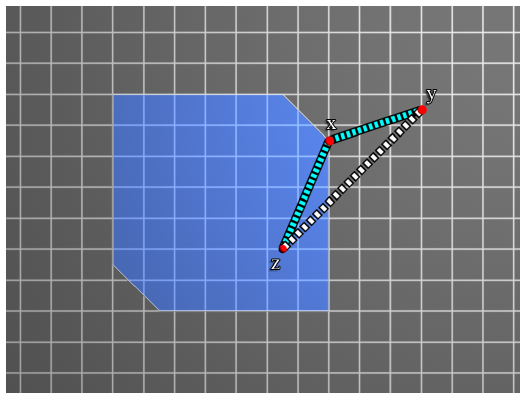
\includegraphics[scale=0.7]{pythagoras}
\caption{An illustration of Pythagoras' theorem. Source: \citep{oco}.}
\label{fig:pythagoras}
\end{figure}
We note that there exists a more general version of Pythagoras' theorem. The above theorem and the definition of projections are true and valid not only for Euclidean norms, but for any norm. In addition, projections according to other distances that are not norms can be defined, in particular with respect to Bregman divergences, and an analogue of Pythagoras' theorem remains valid in such cases.

\subsection{Introduction to optimality conditions}

The standard curriculum of high-school mathematics contains the basic facts about when a function (usually in one dimension) attains a local optimum or saddle point. The generalisation of these conditions to multiple dimensions is called the Karush-Kuhn-Tucker (KKT) conditions, and the reader is referred to \cite{nemirovski, rockafellar, fletcher, bv_cvxbook, borwein, bubeck} for an in-depth rigorous discussion of optimality conditions in general mathematical programming.

We shall only describe briefly and intuitively the main facts that are useful for our purposes. Naturally, we restrict ourselves to convex programming, and thus a local minimum of a convex univariate function is also a global minimum (because the second derivative of a convex function is non-negative everywhere).

The generalisation of the fact that a minimum of a convex differentiable function on $\mathbb{R}$ is a point in which its derivative is equal to zero is given by the multi-dimensional analogue that its gradient is equal to the zero vector:
\begin{equation}
\nabla f(\mathbf{x}) = \mathbf{0}_{d\times 1} \quad \iff \quad \mathbf{x} \in \argmin_{\mathbf{x} \in \mathbb{R}^d} \, f(\mathbf{x}). 
\end{equation}

We will require a slightly more general, but equally intuitive, fact for constrained optimisation: at a minimum point of a constrained convex function, the inner product between the negative gradient and direction towards the interior of $\mathcal{K}$ is non-positive. This is depicted in Figure~\ref{fig:optimality-conditions}, which shows that $-\nabla f(\mathbf{x}^*)$ defines a supporting hyperplane to $\mathcal{K}$. The intuition is that if the inner product were positive, one could improve the objective by moving in the direction of the projected negative gradient. This fact is stated formally in the following theorem.
\begin{figure}[t]
\centering
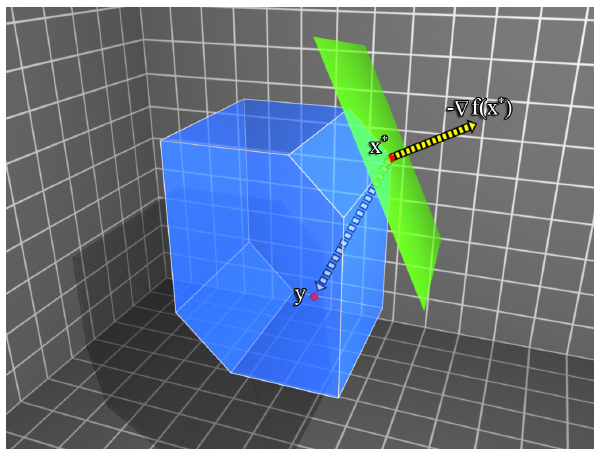
\includegraphics[scale=0.7]{optimality-conditions}
\caption{Optimality conditions: negative gradient pointing outwards. Source: \citep{oco}.}
\label{fig:optimality-conditions}
\end{figure}
\begin{theorem}[Karush-Kuhn-Tucker]
\label{thm:kkt}
Let $\mathcal{K} \subseteq \mathbb{R}^d$ be a convex set, $\mathbf{x}^* \in \argmin_{\mathbf{x} \in \mathcal{K}} \, f(\mathbf{x})$. Then, for any $\mathbf{y} \in \mathcal{K}$, we have
\begin{equation}
\nabla f(\mathbf{x}^*) \cdot (\mathbf{y} - \mathbf{x}^*) \geq 0.
\end{equation}
\end{theorem}


%\section{Gaussian Identities}
%\label{sec:gaussian-identities}
%
%The following identities \citep{rasmussen06} are almost indispensable when dealing with Gaussian distributions, which we denote in the usual way as
%\begin{equation}
%\label{eq:gaussian-pdf-def}
%	\mathcal{N}(\mathbf{x}|\boldsymbol{\mu},\, \boldsymbol{\Sigma})
%	\equiv \frac{1}{\sqrt{|2\pi\boldsymbol{\Sigma}|}}\exp\Big\{-\frac{1}{2}(\mathbf{x} - \boldsymbol{\mu})^\text{T}\boldsymbol{\Sigma}^{-1}(\mathbf{x} - \boldsymbol{\mu})\Big\}.
%\end{equation}
%
%\subsection{Completing the square}
%
%A useful technique in manipulating Gaussians is the so-called technique of `completing the square'. For example, the expression
%\begin{equation}
%	\exp\Big\{-\frac{1}{2}\mathbf{x}^\text{T}\mathbf{A}\mathbf{x} + \mathbf{b}^\text{T}\mathbf{x}\Big\}
%\end{equation}
%can be transformed as follows. First, we complete the square with respect to $\mathbf{x}$ in the exponent:
%\begin{equation}
%	\frac{1}{2}\mathbf{x}^\text{T}\mathbf{A}\mathbf{x} - \mathbf{b}^\text{T}\mathbf{x}
%	= \frac{1}{2}(\mathbf{x} - \mathbf{A}^{-1}\mathbf{b})^\text{T}\mathbf{A}(\mathbf{x} - \mathbf{A}^{-1}\mathbf{b}) - \frac{1}{2}\mathbf{b}^\text{T}\mathbf{A}^{-1}\mathbf{b}.
%\end{equation}
%Hence,
%\begin{equation}
%	\exp\Big\{-\frac{1}{2}\mathbf{x}^\text{T}\mathbf{A}\mathbf{x} + \mathbf{b}^\text{T}\mathbf{x}\Big\}
%	= \mathcal{N}(\mathbf{x}|\mathbf{A}^{-1}\mathbf{b},\, \mathbf{A}^{-1})\sqrt{|2\pi\mathbf{A}^{-1}|}\exp\Big\{\frac{1}{2}\mathbf{b}^\text{T}\mathbf{A}^{-1}\mathbf{b}\Big\}.
%\end{equation}
%From this, one can derive
%\begin{equation}
%	\int \exp\Big\{-\frac{1}{2}\mathbf{x}^\text{T}\mathbf{A}\mathbf{x} + \mathbf{b}^\text{T}\mathbf{x}\Big\}\,\mathrm{d}\mathbf{x}
%	= \sqrt{|2\pi\mathbf{A}^{-1}|}\exp\Big\{\frac{1}{2}\mathbf{b}^\text{T}\mathbf{A}^{-1}\mathbf{b}\Big\}.
%\end{equation}
%
%\subsection{Product of two Gaussians}
%
%The product of two Gaussians is another Gaussian, with a multiplicative factor:
%\begin{equation}
%\label{eq:product-of-2-gaussians}
%	\mathcal{N}(\mathbf{x}|\boldsymbol{\mu}_1,\, \boldsymbol{\Sigma}_1)\,\mathcal{N}(\mathbf{x}|\boldsymbol{\mu}_2,\, \boldsymbol{\Sigma}_2)
%	= \mathcal{N}(\mathbf{x}|\boldsymbol{\mu},\, \boldsymbol{\Sigma})\frac{\exp\big\{-\frac{1}{2}(\boldsymbol{\mu}_1 - \boldsymbol{\mu}_2)^\text{T}\mathbf{S}^{-1}(\boldsymbol{\mu}_1 - \boldsymbol{\mu}_2)\big\}}{\sqrt{|2\pi\mathbf{S}|}},
%\end{equation}
%where $\mathbf{S} \equiv \boldsymbol{\Sigma}_1 + \boldsymbol{\Sigma}_2$ and the mean and covariance are given by
%\begin{equation}
%	\boldsymbol{\mu}
%	= \boldsymbol{\Sigma}(\boldsymbol{\Sigma}_1^{-1}\boldsymbol{\mu}_1 + \boldsymbol{\Sigma}_2^{-1}\boldsymbol{\mu}_2)
%	\qquad \text{and} \qquad
%	\boldsymbol{\Sigma}
%	= (\boldsymbol{\Sigma}_1^{-1} + \boldsymbol{\Sigma}_2^{-1})^{-1}.
%\end{equation}
%Note that the resulting Gaussian has a precision (inverse covariance) equal to the sum of the precisions, and a mean equal to the convex sum of the means, weighted by the precisions.
%
%To prove Eq. \eqref{eq:product-of-2-gaussians}, simply write out the (lengthy) expressions by using the definition \eqref{eq:gaussian-pdf-def} of the Gaussian PDF, and expanding the terms inside the exponential to verify equality (hint: it may be helpful to expand $\boldsymbol{\Sigma}$ using the matrix inversion lemma in Eq. \eqref{eq:woodbury-identity}) 
%
%\subsection{Affine transformations}
%
%Any affine transformation of a Gaussian random vector is itself Gaussian. More precisely, if $\mathbf{y} \equiv \mathbf{A}\mathbf{x} + \mathbf{b}$ and $\mathbf{x} \sim \mathcal{N}(\mathbf{x}|\boldsymbol{\mu},\, \boldsymbol{\Sigma})$, where $\mathbf{x}$ is an $n$-dimensional column vector, $\mathbf{A}$ is a constant $m\times n$ matrix and $\mathbf{b}$ is an $m\times 1$ vector of constants, then $\mathbf{y}$ has multivariate Gaussian distribution with mean $\mathbf{A}\boldsymbol{\mu} + \mathbf{b}$ and covariance $\mathbf{A}\boldsymbol{\Sigma}\mathbf{A}^\text{T}$. In other words,
%\begin{equation}
%	\mathbf{x} \sim \mathcal{N}(\mathbf{x}|\boldsymbol{\mu},\, \boldsymbol{\Sigma})
%	\quad \implies \quad
%	\mathbf{y} \equiv \mathbf{A}\mathbf{x} + \mathbf{b}
%	\sim \mathcal{N}(\mathbf{y}|\mathbf{A}\boldsymbol{\mu} + \mathbf{b},\, \mathbf{A}\boldsymbol{\Sigma}\mathbf{A}^\text{T}).
%\end{equation}
%
%\subsection{Marginal and conditional Gaussians}
%
%Given a marginal Gaussian distribution for $\mathbf{x}$ and a conditional Gaussian distribution for $\mathbf{y}$ given $\mathbf{x}$ in the form
%\begin{align}
%	p(\mathbf{x}) &= \mathcal{N}(\mathbf{x}|\boldsymbol{\mu},\, \boldsymbol{\Lambda}^{-1})
%	\\
%	p(\mathbf{y}|\mathbf{x}) &= \mathcal{N}(\mathbf{y}|\mathbf{A}\mathbf{x} + \mathbf{b},\, \mathbf{L}^{-1})
%\end{align}
%the marginal distribution of $\mathbf{y}$ and the conditional distribution for $\mathbf{x}$ given $\mathbf{y}$ are given by
%\begin{align}
%	p(\mathbf{y}) &= \mathcal{N}(\mathbf{y}|\mathbf{A}\boldsymbol{\mu} + \mathbf{b},\, \mathbf{L}^{-1} + \mathbf{A}\boldsymbol{\Lambda}^{-1}\mathbf{A}^\text{T})
%	\\
%	p(\mathbf{x}|\mathbf{y}) &= \mathcal{N}(\mathbf{x}|\boldsymbol{\Sigma}\{\mathbf{A}^\text{T}\mathbf{L}(\mathbf{y} - \mathbf{b}) + \boldsymbol{\Lambda}\boldsymbol{\mu}\},\, \boldsymbol{\Sigma})
%\end{align} 
%where
%\begin{equation}
%	\boldsymbol{\Sigma} = (\boldsymbol{\Lambda} + \mathbf{A}^\text{T}\mathbf{L}\mathbf{A})^{-1}.
%\end{equation}




\section{Matrix Identities}
\label{sec:matrix-identities}

The \emph{matrix inversion lemma}, also known as the Woodbury, Sherman \& Morrison formula (see e.g.\ \citep[p.~75]{press92}) states that
\begin{equation}
\label{eq:woodbury-identity}
	(\mathbf{Z} + \mathbf{U}\mathbf{W}\mathbf{V}^\text{T})^{-1}
	= \mathbf{Z}^{-1} - \mathbf{Z}^{-1}\mathbf{U}(\mathbf{W}^{-1} + \mathbf{V}^\text{T}\mathbf{Z}^{-1}\mathbf{U})^{-1}\mathbf{V}^\text{T}\mathbf{Z}^{-1},
\end{equation}
assuming the relevant inverses all exist. Here $\mathbf{Z}$ is $n\times n$, $\mathbf{W}$ is $m\times m$ and $\mathbf{U}$ and $\mathbf{V}$ are both of size $n\times m$. Consequently, if $\mathbf{Z}^{-1}$ is known, and a low-rank (i.e.\ $m < n$) perturbation is made to $\mathbf{Z}$ as in the left-hand side of Eq. \eqref{eq:woodbury-identity}, considerable speedup can be achieved.
\chapter{Probability Distributions}
\label{ch:probability-distributions}

\minitoc


This appendix gives the definitions and some properties of the probability distributions used for inference in this thesis. For each distribution, we list some key statistics such as the expectation, the variance (or covariance), and the entropy $\mathrm{H}(x)$.


\section{Uniform Distribution}
\label{sec:uniform-distribution}

The uniform distribution is often used as a non-informative prior, and assigns equal mass to all possible values in the distribution. When the variable is discrete, the probability is trivially set by dividing the total mass by the number of possible discrete values $N$,
\begin{equation}
	p(n) = \frac{1}{N},
\end{equation}
but when the variable is continuous, it can be more difficult to specify a density. Fortunately, when the range of possible values is limited to some interval, the density is given as
\begin{equation}
	\mathcal{U}(x|a, b)
	\equiv \frac{1}{b-a}\mathds{1}_{(a,\, b)}(x)
\end{equation}
which assigns equal mass within the interval and zero mass elsewhere. When a uniform distribution is required over all real values $x \in \mathbb{R}$, the distribution is \emph{improper} since it is impossible to normalise the density.

The mean and variance of the continuous uniform distribution are respectively:
\begin{equation}
\label{eq:uniform-moments}
	\mathbb{E}(x) = \frac{a+b}{2}
	\quad \text{and} \quad
	\mathrm{Var}(x) = \frac{(b-a)^2}{12}.
\end{equation}
An interesting property is that if $x$ has distribution $\mathcal{U}(x|0, 1)$, then $y \equiv a + (b-a)x$ will have distribution $\mathcal{U}(y|a, b)$.


\section{Gamma Distribution}

The Gamma is a probability distribution over a positive random variable $x > 0$ governed by a shape parameter $a$ and a rate parameter $b$ that are subject to the constraints $a > 0$ and $b > 0$ to ensure that the distribution can be normalised.
\begin{align}
	\mathcal{G}(x|a, b)
	&= \frac{b^a}{\Gamma(a)}x^{a-1}\exp\big\{-bx\big\}\mathds{1}_{(0,\,\infty)}(x)
	\label{eq:gamma-density} \\
	\mathbb{E}(x) &= \frac{a}{b}
	\\
	\mathrm{Var}(x) &= \frac{a}{b^2}
	\\
	\mathrm{mode}(x) &= \frac{a-1}{b}
	\qquad \text{for } a \geq 1,
\end{align}
where $\Gamma(a) = \int_{0}^{\infty} x^{a-1}\exp\big\{-x\big\}\,\mathrm{d}x$ is the gamma function.

The Gamma distribution is typically used as a prior for scale parameters (see e.g. \citep{berger85}). An example of scale parameter would be the standard deviation $\sigma$ of a univariate Gaussian distribution, after we have taken account of the location parameter $\mu$. The uninformative prior is obtained as the special case $a = b = 0$, in which $p(x) = \mathcal{G}(x|a, b)$ takes the form $p(x) \propto 1/x$. Using the transformation rule \eqref{eq:pdf-chg-of-vars} for densities, we see that this leads to a uniform prior over the logarithmic scale, i.e.\ $p(\log x) = \text{const}$.


\section{Shifted Exponential Distribution}
\label{sec:shifted-exponential-distribution}

An important special case of the Gamma distribution is the exponential distribution, whose density is obtained by setting $a = 1$ in Eq. \eqref{eq:gamma-density}:
\begin{equation}
	\mathcal{E}(x|\lambda)
	= \lambda\exp\Big\{-\lambda x\Big\}\mathds{1}_{(0,\,\infty)}(x),
\end{equation}
with $\lambda = \beta$. The exponential distribution is used to describe the time between events in a Poisson point process, i.e.\ a process in which events occur continuously and independently at a constant average rate $\lambda$.

If we shift the origin of an exponentially distributed random variable, then we obtain the so-called shifted exponential distribution, whose density is given by
\begin{equation}
	\mathcal{E}(x|\lambda, \theta)
	= \lambda\exp\Big\{-\lambda(x - \theta)\Big\}\mathds{1}_{(\theta,\, \infty)}(x),
\end{equation}
where, as before, $\lambda > 0$ is the rate parameter, while $\theta \in \mathbb{R}$ is the location parameter. The shifted exponential distribution is widely used in the analysis of lifetime or response time data that arises in areas such as product performance evaluation and clinical trials \citep{bain78, lawless82}. Using integration by parts, it is straightforward to show that its mean and variance are respectively:
\begin{equation}
\label{eq:shifted-exponential-moments}
	\mathbb{E}(x) = \frac{1}{\lambda} + \theta,
	\qquad
	\mathrm{Var}(x) = \frac{1}{\lambda^2}.
\end{equation}
Note that the variance coincides with that of the non-shifted exponential distribution, which is not surprising given that the variance is invariant to translations.


\section{Gaussian Distribution}

The Gaussian is the most widely used distribution for continuous variables. It is also known as the \emph{normal} distribution. In the case of a single variable $x \in \mathbb{R}$, it is governed by two parameters, the mean $\mu \in \mathbb{R}$ and the variance $\sigma^2 > 0$.
\begin{align}
	\mathcal{N}(x|\mu,\, \sigma^2)
	&= \frac{1}{\sqrt{2\pi\sigma^2}}\exp\Big\{-\frac{1}{2\sigma^2}(x - \mu)^2\Big\}
	\\
	\mathbb{E}(x) &= \mu
	\\
	\mathrm{Var}(x) &= \sigma^2
	\\
	\mathrm{mode}(x) &= \mu
	\\
	\mathrm{H}(x)
	&= \frac{1}{2}\log\sigma^2 + \frac{1}{2}[1 + \log(2\pi)].
\end{align}
The inverse of the variance $\beta = 1/\sigma^2$ is called the precision, and the square root of the variance, $\sigma$, is called the standard deviation.

For an $n$-dimensional column vector $\mathbf{x}$, the Gaussian is governed by an $n$-dimensional (column) mean vector $\boldsymbol{\mu}$ and an $n\times n$ covariance matrix $\boldsymbol{\Sigma}$ that must be symmetric and positive-definite.
\begin{align}
	\mathcal{N}(\mathbf{x}|\boldsymbol{\mu},\, \boldsymbol{\Sigma})
	&= (2\pi)^{-n/2}|\boldsymbol{\Sigma}|^{-1/2}\exp\Big\{-\frac{1}{2}(\mathbf{x} - \boldsymbol{\mu})^\text{T}\boldsymbol{\Sigma}^{-1}(\mathbf{x} - \boldsymbol{\mu})\Big\}
	\label{eq:gaussian-pdf-def} \\
	\mathbb{E}(\mathbf{x}) &= \boldsymbol{\mu}
	\\
	\mathrm{Cov}(\mathbf{x}) &= \boldsymbol{\Sigma}
	\\
	\mathrm{mode}(\mathbf{x}) &= \boldsymbol{\mu}
	\\
	\mathrm{H}(\mathbf{x})
	&= \frac{1}{2} \log|\boldsymbol{\Sigma}| + \frac{n}{2}[1 + \log(2\pi)].
	\label{eq:multivariate-gaussian-entropy}
\end{align}
The inverse of the covariance matrix $\boldsymbol{\Lambda} = \boldsymbol{\Sigma}^{-1}$ is the precision matrix, which is also symmetric and positive definite. Averages of random variables tend to a Gaussian, by the central limit theorem, and the sum of two Gaussian variables is again Gaussian. The Gaussian is the distribution that maximises the entropy for a given variance (or covariance).

Any linear transformation of a Gaussian random variable is again a Gaussian. The marginal distribution of a multivariate Gaussian with respect to a subset of the variables is itself Gaussian, and similarly the conditional distribution is also Gaussian. See below for details.

\subsection{Properties}
\label{sec:gaussian-identities}

The following properties \citep{rasmussen06, barber} are almost indispensable when dealing with Gaussian distributions.

\subsubsection{Completing the square}

A useful technique in manipulating Gaussians is the so-called technique of `completing the square'. For example, the expression
\begin{equation}
	\exp\Big\{-\frac{1}{2}\mathbf{x}^\text{T}\mathbf{A}\mathbf{x} + \mathbf{b}^\text{T}\mathbf{x}\Big\}
\end{equation}
can be transformed as follows. First, we complete the square with respect to $\mathbf{x}$ in the exponent:
\begin{equation}
	\frac{1}{2}\mathbf{x}^\text{T}\mathbf{A}\mathbf{x} - \mathbf{b}^\text{T}\mathbf{x}
	= \frac{1}{2}(\mathbf{x} - \mathbf{A}^{-1}\mathbf{b})^\text{T}\mathbf{A}(\mathbf{x} - \mathbf{A}^{-1}\mathbf{b}) - \frac{1}{2}\mathbf{b}^\text{T}\mathbf{A}^{-1}\mathbf{b}.
\end{equation}
Hence,
\begin{equation}
	\exp\Big\{-\frac{1}{2}\mathbf{x}^\text{T}\mathbf{A}\mathbf{x} + \mathbf{b}^\text{T}\mathbf{x}\Big\}
	= \mathcal{N}(\mathbf{x}|\mathbf{A}^{-1}\mathbf{b},\, \mathbf{A}^{-1})\sqrt{|2\pi\mathbf{A}^{-1}|}\exp\Big\{\frac{1}{2}\mathbf{b}^\text{T}\mathbf{A}^{-1}\mathbf{b}\Big\}.
\end{equation}
From this, one can derive
\begin{equation}
	\int \exp\Big\{-\frac{1}{2}\mathbf{x}^\text{T}\mathbf{A}\mathbf{x} + \mathbf{b}^\text{T}\mathbf{x}\Big\}\,\mathrm{d}\mathbf{x}
	= \sqrt{|2\pi\mathbf{A}^{-1}|}\exp\Big\{\frac{1}{2}\mathbf{b}^\text{T}\mathbf{A}^{-1}\mathbf{b}\Big\}.
\end{equation}

\subsubsection{Product of two Gaussians}

The product of two Gaussians is another Gaussian, with a multiplicative factor:
\begin{equation}
\label{eq:product-of-2-gaussians}
	\mathcal{N}(\mathbf{x}|\boldsymbol{\mu}_1,\, \boldsymbol{\Sigma}_1)\,\mathcal{N}(\mathbf{x}|\boldsymbol{\mu}_2,\, \boldsymbol{\Sigma}_2)
	= \mathcal{N}(\mathbf{x}|\boldsymbol{\mu},\, \boldsymbol{\Sigma})\frac{\exp\big\{-\frac{1}{2}(\boldsymbol{\mu}_1 - \boldsymbol{\mu}_2)^\text{T}\mathbf{S}^{-1}(\boldsymbol{\mu}_1 - \boldsymbol{\mu}_2)\big\}}{\sqrt{|2\pi\mathbf{S}|}},
\end{equation}
where $\mathbf{S} \equiv \boldsymbol{\Sigma}_1 + \boldsymbol{\Sigma}_2$ and the mean and covariance are given by
\begin{equation}
	\boldsymbol{\mu}
	= \boldsymbol{\Sigma}(\boldsymbol{\Sigma}_1^{-1}\boldsymbol{\mu}_1 + \boldsymbol{\Sigma}_2^{-1}\boldsymbol{\mu}_2)
	\qquad \text{and} \qquad
	\boldsymbol{\Sigma}
	= (\boldsymbol{\Sigma}_1^{-1} + \boldsymbol{\Sigma}_2^{-1})^{-1}.
\end{equation}
Note that the resulting Gaussian has a precision (inverse covariance) equal to the sum of the precisions, and a mean equal to the convex sum of the means, weighted by the precisions.

To prove Eq. \eqref{eq:product-of-2-gaussians}, simply write out the (lengthy) expressions by using the definition \eqref{eq:gaussian-pdf-def} of the Gaussian PDF, and expanding the terms inside the exponential to verify equality (hint: it may be helpful to expand $\boldsymbol{\Sigma}$ using the matrix inversion lemma in Eq. \eqref{eq:woodbury-identity}) 

\subsubsection{Affine transformations}

Any affine transformation of a Gaussian random vector is itself Gaussian. More precisely, if $\mathbf{y} \equiv \mathbf{A}\mathbf{x} + \mathbf{b}$ and $\mathbf{x} \sim \mathcal{N}(\mathbf{x}|\boldsymbol{\mu},\, \boldsymbol{\Sigma})$, where $\mathbf{x}$ is an $n$-dimensional column vector, $\mathbf{A}$ is a constant $m\times n$ matrix and $\mathbf{b}$ is an $m\times 1$ vector of constants, then $\mathbf{y}$ has multivariate Gaussian distribution with mean $\mathbf{A}\boldsymbol{\mu} + \mathbf{b}$ and covariance $\mathbf{A}\boldsymbol{\Sigma}\mathbf{A}^\text{T}$. In other words,
\begin{equation}
	\mathbf{x} \sim \mathcal{N}(\mathbf{x}|\boldsymbol{\mu},\, \boldsymbol{\Sigma})
	\quad \implies \quad
	\mathbf{y} \equiv \mathbf{A}\mathbf{x} + \mathbf{b}
	\sim \mathcal{N}(\mathbf{y}|\mathbf{A}\boldsymbol{\mu} + \mathbf{b},\, \mathbf{A}\boldsymbol{\Sigma}\mathbf{A}^\text{T}).
\end{equation}

\subsubsection{Partitioned Gaussians}

Perhaps the most important property of a multivariate Gaussian distribution is that its marginals and conditionals are both themselves Gaussian. That is, if we have a joint Gaussian distribution $\mathcal{N}(\mathbf{x}|\boldsymbol{\mu},\, \boldsymbol{\Sigma})$ with $\boldsymbol{\Lambda} \equiv \boldsymbol{\Sigma}^{-1}$ and we define the following partitions
\begin{align}
	& \mathbf{x} =
	\begin{pmatrix}
		\mathbf{x}_a \\
		\mathbf{x}_b
	\end{pmatrix},
	\qquad
	\boldsymbol{\mu} =
	\begin{pmatrix}
		\boldsymbol{\mu}_a \\
		\boldsymbol{\mu}_b
	\end{pmatrix}
	\\
	& \boldsymbol{\Sigma} =
	\begin{bmatrix}
		\boldsymbol{\Sigma}_{aa} & \boldsymbol{\Sigma}_{ab} \\
		\boldsymbol{\Sigma}_{ba} & \boldsymbol{\Sigma}_{bb}
	\end{bmatrix},
	\qquad
	\boldsymbol{\Lambda} =
	\begin{bmatrix}
		\boldsymbol{\Lambda}_{aa} & \boldsymbol{\Lambda}_{ab} \\
		\boldsymbol{\Lambda}_{ba} & \boldsymbol{\Lambda}_{bb}
	\end{bmatrix}	
\end{align}
then the conditional distribution $p(\mathbf{x}_a|\mathbf{x}_b)$ is given by
\begin{equation}
	p(\mathbf{x}_a|\mathbf{x}_b)
	= \mathcal{N}(\mathbf{x}_a|\boldsymbol{\mu}_{a|b},\, \boldsymbol{\Lambda}_{aa}^{-1}),
	\qquad
	\boldsymbol{\mu}_{a|b}
	= \boldsymbol{\mu}_{a} - \boldsymbol{\Lambda}_{aa}^{-1}\boldsymbol{\Lambda}_{ab}(\mathbf{x}_b - \boldsymbol{\mu}_{b})
\end{equation}
and the marginal $p(\mathbf{x}_a)$ is given by
\begin{equation}
	p(\mathbf{x}_a)
	= \mathcal{N}(\mathbf{x}_a|\boldsymbol{\mu}_{a},\, \boldsymbol{\Sigma}_{aa}).
\end{equation}

\subsubsection{Marginal and conditional Gaussians}

We now turn to another important property of the Gaussian distribution, illustrated in Figure~\ref{fig:mosb}.
\begin{figure}
\centering
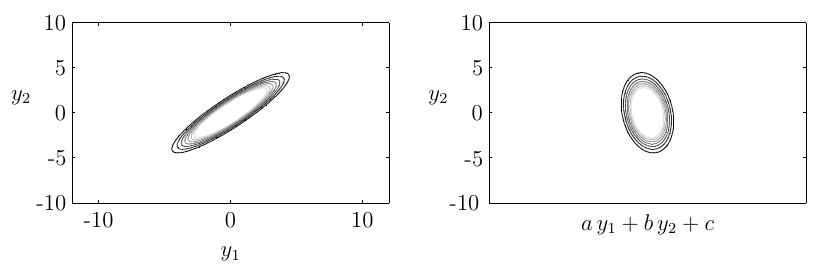
\includegraphics[scale=0.7]{mosb}
\caption{Any variables over which we have a multivariate Gaussian are jointly Gaussian with any linear transformation of those variables. Source: \citep{mosb}.}
\label{fig:mosb}
\end{figure}
Given a marginal Gaussian distribution for $\mathbf{x}$ and a conditional Gaussian distribution for $\mathbf{y}$ given $\mathbf{x}$ in the form
\begin{align}
	p(\mathbf{x}) &= \mathcal{N}(\mathbf{x}|\boldsymbol{\mu},\, \boldsymbol{\Lambda}^{-1})
	\\
	p(\mathbf{y}|\mathbf{x}) &= \mathcal{N}(\mathbf{y}|\mathbf{A}\mathbf{x} + \mathbf{b},\, \mathbf{L}^{-1})
\end{align}
the marginal distribution of $\mathbf{y}$ and the conditional distribution for $\mathbf{x}$ given $\mathbf{y}$ are given by
\begin{align}
	p(\mathbf{y}) &= \mathcal{N}(\mathbf{y}|\mathbf{A}\boldsymbol{\mu} + \mathbf{b},\, \mathbf{L}^{-1} + \mathbf{A}\boldsymbol{\Lambda}^{-1}\mathbf{A}^\text{T})
	\\
	p(\mathbf{x}|\mathbf{y}) &= \mathcal{N}(\mathbf{x}|\boldsymbol{\Sigma}\{\mathbf{A}^\text{T}\mathbf{L}(\mathbf{y} - \mathbf{b}) + \boldsymbol{\Lambda}\boldsymbol{\mu}\},\, \boldsymbol{\Sigma})
\end{align} 
where
\begin{equation}
	\boldsymbol{\Sigma} = (\boldsymbol{\Lambda} + \mathbf{A}^\text{T}\mathbf{L}\mathbf{A})^{-1}.
\end{equation}

\subsubsection{Gaussian average of a quadratic function}

Last but not least, the following result is also useful:
\begin{equation}
\label{eq:gaussian-avg-of-quadratic-fct}
	\langle\mathbf{x}^\text{T}\mathbf{A}\mathbf{x}\rangle_{\mathcal{N}(\mathbf{x}|\boldsymbol{\mu},\, \boldsymbol{\Sigma})}
	= \boldsymbol{\mu}^\text{T}\mathbf{A}\boldsymbol{\mu}
	+ \mathrm{Tr}(\mathbf{A}\boldsymbol{\Sigma}).
\end{equation}

\section{Generalised Gaussian Distribution}
\label{sec:generalised-gaussian-distribution}

The generalised inverse Gaussian distribution (GIG) is a three-parameter family of continuous probability distributions with probability density function
\begin{equation}
	\mathcal{GIG}(x|\delta, \chi, \psi)
	= \frac{(\psi/\chi)^{\delta/2}}{2K_{\delta}(\sqrt{\psi\chi})}x^{\delta-1}\exp\Big\{-\frac{1}{2}\left(\psi x + \frac{\chi}{x}\right)\Big\}\mathds{1}_{(0,\, \infty)}(x),
\end{equation}
where $K_{\delta}(\cdot)$ denotes the modified Bessel function of the second kind with index $\delta \in \mathbb{R}$, and $\chi, \psi > 0$. It is used extensively in geostatistics, statistical linguistics, finance, etc. Its statistical properties, and in particular the following lemma, can be found in \citep{jorgensen82}.
\begin{lemma}
\label{lem:jorgensen}
Let $x$ be distributed according to $\mathcal{GIG}(x|\delta, \chi, \psi)$, with $\psi > 0$ and $\chi > 0$. Then
\begin{equation}
	\mathbb{E}(x^p)
	= \left(\frac{\chi}{\psi}\right)^{p/2}\frac{K_{\delta+p}(\sqrt{\psi\chi})}{K_{\delta}(\sqrt{\psi\chi})}.
\end{equation}
\end{lemma}
An immediate consequence of this lemma that turns out to be useful for our purposes is given below. 
\begin{corollary}
\label{cor:jorgensen}
If $x$ is distributed according to $\mathcal{GIG}(x|1/2, \chi, \psi)$, where $\psi > 0$ and $\chi > 0$, then
\begin{align}
	\mathbb{E}(x)
	= \frac{1 + \sqrt{\psi\chi}}{\psi},
	\qquad
	\mathbb{E}(x^{-1})
	= \sqrt{\frac{\psi}{\chi}}.
\end{align}
\end{corollary}
It is straightforward to prove this corollary, by combining Lemma~\ref{lem:jorgensen} with the following one from \citep{abramowitz}.
\begin{lemma}
\label{lem:abramowitz}
The modified Bessel function of the second kind, $K_{\delta}(\cdot)$, satisfies the following properties:
\begin{enumerate}
	\item $K_{\delta}(x) = K_{-\delta}(x)$;
	\item $K_{\delta+1}(x) = 2\frac{\delta}{x}K_{\delta}(x) + K_{\delta-1}(x)$;
	\item $K_{1/2}(x) = K_{-1/2}(x) = \sqrt{\frac{\pi}{2x}}\exp\{-x\}$.
\end{enumerate}
\end{lemma}

\subsection{Entropy}

Using Lemmata~\ref{lem:jorgensen} and~\ref{lem:abramowitz}, the entropy of the generalised inverse Gaussian distribution is given as
\begin{align}
	\mathrm{H}(x)
	&= \frac{\delta}{2}\log\frac{\chi}{\psi} + \log\big[2K_{\delta}\big(\sqrt{\psi\chi}\big)\big] - (\delta-1)\langle\,\log x\,\rangle
	\nonumber \\
	& \quad + \frac{\sqrt{\psi\chi}}{2K_{\delta}(\sqrt{\psi\chi})}\big[K_{\delta+1}\big(\sqrt{\psi\chi}\big) + K_{\delta-1}\big(\sqrt{\psi\chi}\big)\big]
	\\	
	&= \frac{\delta}{2}\log\frac{\chi}{\psi} + \log\big[2K_{\delta}\big(\sqrt{\psi\chi}\big)\big] - (\delta-1)\frac{\frac{\mathrm{d}}{\mathrm{d}\nu}K_{\nu}(\sqrt{\psi\chi})\big|_{\nu=\delta}}{K_{\delta}(\sqrt{\psi\chi})}
	\nonumber \\
	& \quad + \frac{\sqrt{\psi\chi}}{2K_{\delta}(\sqrt{\psi\chi})}\big[K_{\delta+1}\big(\sqrt{\psi\chi}\big) + K_{\delta-1}\big(\sqrt{\psi\chi}\big)\big],
	\nonumber
\end{align}
where $\frac{\mathrm{d}}{\mathrm{d}\nu}K_{\nu}(\sqrt{\psi\chi})\big|_{\nu=\delta}$ is the derivate of the modified Bessel function of the second kind with respect to its order $\nu$, evaluated at $\nu=\delta$. In particular, when $\delta = 1/2$, this boils down to
\begin{equation}
\label{eq:gig-entropy}
	\mathrm{H}(x)
	= \frac{1}{2}\left(1 - \log\frac{\psi}{2\pi}\right) - (\delta-1)\langle\,\log x\,\rangle,
\end{equation}
which is easily proved by making use of Lemma~\ref{lem:abramowitz}.

\subsection{Special cases}

It is well know that the special cases of the GIG distribution include the Gamma distribution $\mathcal{G}(x|\delta, \psi/2)$ when $\chi = 0$ and $\delta > 0$, the inverse Gamma distribution $\mathcal{IG}(x|-\delta, \chi/2)$ when $\psi = 0$ and $\delta < 0$, the inverse Gaussian distribution when $\delta = -1/2$, and the hyperbolic distribution when $\delta = 0$. We refer the reader to \citep{jorgensen82} for details.

Note in particular that the PDF of the inverse Gaussian $\mathcal{GIG}(x|1/2, \chi, \psi)$ is
\begin{equation}
\label{eq:gig-pdf-for-delta-1/2}
	p(x)
	= \sqrt{\frac{\psi}{2\pi}}\exp\Big\{\sqrt{\psi\chi}\Big\}x^{-1/2}\exp\Big\{-\frac{1}{2}\left(\psi x + \frac{\chi}{x}\right)\Big\}\mathds{1}_{(0,\, \infty)}(x).
\end{equation}


%%%%% REFERENCES
\bibliography{references}
\bibliographystyle{plainnat}


\end{document}